% $Id$

\documentclass[a4paper,titlepage]{book}
% \documentclass[draft]{book}
\usepackage{epsfig,amsmath,pifont,moreverb,minitoc,alltt}
\usepackage[
	colorlinks=true,
	pdfpagemode=UseOutlines,
	pdftitle={PRoNTo Manual},
	pdfauthor={The PRoNTo Team},
	pdfsubject={Pattern Recognition in Neuroimaging Toolbox},
	pdfkeywords={neuroimaging, data mining, multivariate analysis, pattern recognition}
	]{hyperref}
\usepackage[usenames,dvipsnames]{color}
\hypersetup{
 colorlinks,
 citecolor=PineGreen,
 linkcolor=NavyBlue,
 urlcolor=NavyBlue}
\usepackage[titles]{tocloft}
\usepackage{subcaption}
\usepackage{silence}
\WarningFilter{latex}{Text page}

% \usepackage[T1]{fontenc} % NOT USED
% \usepackage{bigfoot} % to allow verbatim in footnote % NOT USED
\usepackage{listings}
% \usepackage[numbered,framed]{matlab-prettifier} % NOT USED

\definecolor{mygreen}{RGB}{28,172,0} % color values Red, Green, Blue
\definecolor{mylilas}{RGB}{170,55,241}
\lstset{language=Matlab,%
    %basicstyle=\color{red},
    breaklines=true,%
    morekeywords={matlab2tikz},
    keywordstyle=\color{blue},%
    morekeywords=[2]{1}, keywordstyle=[2]{\color{black}},
    identifierstyle=\color{black},%
    stringstyle=\color{mylilas},
    commentstyle=\color{mygreen},%
    showstringspaces=false,%without this there will be a symbol in the places where there is a space
    numbers=left,%
    numberstyle={\tiny \color{black}},% size of the numbers
    numbersep=9pt, % this defines how far the numbers are from the text
    emph=[1]{for,end,break},emphstyle=[1]\color{red}, %some words to emphasise
    %emph=[2]{word1,word2}, emphstyle=[2]{style},    
}

\pagestyle{headings}
\bibliographystyle{plain}

%-----------------------------------------------------------------------

\hoffset=-6mm
\voffset=-5mm
\oddsidemargin=0mm
\evensidemargin=0mm
\topmargin=0mm
\headheight=12pt
\headsep=10mm
\textheight=240mm
\textwidth=170mm
\marginparsep=5mm
\marginparwidth=21mm
\footskip=10mm

%-----------------------------------------------------------------------
\title{\huge{PRoNTo Manual}}
\author{The PRoNTo Team}

%-----------------------------------------------------------------------
% Defining some new commands & character sequences
\newcommand{\bi}{\begin{itemize}}
\newcommand{\ei}{\end{itemize}}
\newcommand{\matlab}{\textsc{Matlab}}
\newcommand{\bslash}{\texttt{\symbol{92}}}

% extra space between section number & name in TOC
\renewcommand*\cftsecnumwidth{3em}
\renewcommand*\cftsubsecnumwidth{4em}

%\newcommand{\PRoNTo}{\textsc{PRoNTo}}
%\newcommand{\PRoNTo}{{\it PRoNTo} }
\def\PRoNTo{\hbox{\it P\hskip -1.5pt R\hskip -1.5pt o\hskip -1.5pt N\hskip -1.5pt T\hskip -1.5pt o }}
\def\HPRoNTo{\hbox{\it P\hskip -4.5pt R\hskip -4.5pt o\hskip -4.5pt N\hskip -4.5pt T\hskip -4.5pt o }}
\def\hPRoNTo{\hbox{\it P\hskip -3.5pt R\hskip -3.5pt o\hskip -3.5pt N\hskip -3.5pt T\hskip -3.5pt o }}


%==========================================
%==========================================
\begin{document}

\let\oldlabel=\label
\renewcommand{\label}[1]{
{\pdfdest name {#1} fit}
\oldlabel{#1}
}

%-----------------------------------------------------------------------

%\maketitle
\newlength{\centeroffset}
\setlength{\centeroffset}{-0.5\oddsidemargin}
\addtolength{\centeroffset}{0.5\evensidemargin}
\thispagestyle{empty}


\vspace*{\stretch{1}}
\noindent\hspace*{\centeroffset}\makebox[0pt][l]{\begin{minipage}{\textwidth}
\flushright
\color{NavyBlue}
\textbf{\Huge{\HPRoNTo Manual}}
{\noindent\rule[-1ex]{\textwidth}{5pt}\\[2.5ex]}
\hfill{{\huge The \hPRoNTo Development Group} \\
\Large{(and honorary members)}\\}
\vspace{20mm}
\hfill{
John Ashburner\\
Carlton Chu\\
Andre Marquand\\
Janaina Mourao-Miranda\\
Joao M. Monteiro\\
Christophe Phillips\\
Anil Rao\\
Jonas Richiardi\\
Jane Rondina\\
Maria J. Rosa\\
Jessica Schrouff\\
Konstantinos Tsirlis\\
Tong Wu\\
}
\end{minipage}}

\begin{figure*}[h!]
  
\includegraphics[scale=0.7]{images/Logo_man.png}
\end{figure*}

\vspace{\stretch{1}}
\noindent\hspace*{\centeroffset}\makebox[0pt][l]{\begin{minipage}{\textwidth}
\flushright
\color{NavyBlue}
{\footnotesize
\underline{\textbf{This is a beta version and is subject to change.}}\\
\vspace{5mm}
Machine Learning \& Neuroimaging Laboratory\\
Centre for Medical Image Computing\\
Computer Science Department, UCL\\
90 High Holborn, Holborn, London WC1V 6LJ, UK \\
\today\\
\url{http://www.mlnl.cs.ucl.ac.uk/pronto}}

\end{minipage}}

%-----------------------------------------------------------------------

\dominitoc 
%\hypersetup{linkcolor=NavyBlue}
\tableofcontents
\newpage

%%%%%% INTRODUCTION %%%%%%s
%==========================================
% $Id$

\chapter{Introduction}
\label{chap:intro}
\minitoc

%==========================
\section{Background}
%==========================

Advances in neuroimaging techniques have radically changed the way neuroscientists address questions about functional anatomy, especially in relation to behavioural and clinical disorders. Many questions about brain function, previously investigated using intracranial electrophysiological recordings in animals can now be addressed non-invasively in humans. Such studies have yielded important results in cognitive neuroscience and neuropsychology. Amongst the various neuroimaging modalities available, Magnetic Resonance Imaging (MRI) has become widely used due to its relatively high spatial and temporal resolution, and because it is safe and non-invasive. By selecting specific MRI sequence parameters, different MR signals can be obtained from different tissue types, giving images with high contrast among organs, between normal and abnormal tissues and/or between activated and deactivated brain areas. MRI is often sub-categorized into structural MRI (MRI) and functional MRI (fMRI). Positron Emission Tomography (PET) is another example of neuroimaging modality which measures metabolic processes. Examples of other of imaging modalities that measure  brain signals are ElectroEncephaloGraphy (EEG) recordings and MagnetoEncephaloGraphy (MEG) recordings. Neuroimaging data are inherently multivariate, since each measure (scan or recording) contains information from thousands of locations (e.g. voxels in MRI or electrodes in EEG). Considering that most brain functions are distributed processes involving a network of brain regions, it would seem desirable to use the spatially distributed information contained in the data to give a better understanding of brain functions in normal and abnormal conditions.
\\

The typical analysis pipeline in neuroimaging is strongly rooted in a mass-univariate statistical approach, which assumes that activity in one brain region occurs independently from activity in other regions. Although this has yielded great insights over the years, specially in terms of function localization, and continues to be the tool of choice for data analysis, there is a growing recognition that the spatial dependencies among signal from different brain regions should be properly modelled. The effect of interest can be subtle and spatially distributed over the brain - a case of high-dimensional, multivariate data modelling for which conventional tools may lack sensitivity. 
\\

Therefore, there has been an increasing interest in investigating this spatially distributed information using multivariate pattern recognition approaches, often referred to as  multi-voxel pattern analysis (MVPA) (see  \cite{Norman2006},  \cite{Haynes2006} and \cite{Pereira2009}). Where pattern recognition has been used in neuroimaging, it has led to fundamental advances in the understanding of how the brain represents information and has been applied to many diagnostic problems. For the latter, this approach can be used to predict the group membership of the patient scanned (healthy vs. patients or disease A vs. B) and can provide the discriminating pattern leading to this classification. Pattern recognition techniques can also be used to identify relationships between patterns of brain structure or activity and continuous measures such as age or a clinical score. Such information can then be used to predict individual-level measures for new individuals (i.e. regression models).
\\

Several active areas of research in machine learning are crucially important for the difficult problem of neuroimaging data analysis: modelling of high-dimensional multivariate time series, sparsity, regularisation, dimensionality reduction, causal modelling, and ensembling to name a few. However, the application of pattern recognition approaches to the analysis of neuroimaging data is limited mainly by the lack of user-friendly and comprehensive tools available to the fundamental, cognitive, and clinical neuroscience communities. Furthermore, it is not uncommon for these methods to be used incorrectly, with the most typical case being improper separation of training and testing datasets.
\\

\noindent \textbf{Note:} PRoNTo (Pattern Recognition for Neuroimaging Toolbox) is first and foremost a machine learning tool used for neuroimaging analyses, so throughout the manual we mostly refer to examples that focus on neuroimaging data. That being said, since from the current release PRoNTo supports MEEG (SPM) data as well as any .mat file, one can use PRoNTo to analyze for example MEEG data in sensor space (2D, or even 1D), or yet any kind of .mat file, such as behavior data. However, it is best to use PRoNTo primarily for neuroimaging data which is its original purpose or to build multi-modal predictive models including imaging and non-imaging information. So from the current release, we will refer to our data with the general term `samples' and `features', instead of referring to `voxels' as our features. The reason is that from the current release we have expanded our functionalities to include data that are not 3D, and therefore they do not have `voxels' as features.
\\

%==========================
\section{Methods}
%==========================

PRoNTo (Pattern Recognition for Neuroimaging Toolbox) is a toolbox based on pattern recognition techniques for the analysis of neuroimaging data. Statistical pattern recognition is a field within the area of machine learning which is concerned with automatic discovery of regularities in data through the use of computer algorithms, and with the use of these regularities to take actions such as classifying the data into different categories \cite{Bishop2006}. In PRoNTo, brain images are treated as spatial patterns and statistical learning models are used to identify statistical properties of the data that can be used to discriminate between experimental conditions or groups of subjects (classification models) or to predict a continuous measure (regression models).
\\

PRoNTo is \matlab-based and includes six main modules: `Data \& Design', `Prepare feature set', `Model: Specify new', `Model: Specify from', `Model: Run' and `Compute weights'. For a specific model PRoNTo can display results in terms of performance as well as  the model's weights. Additional review options enable the user to review information about the data, features and models. All modules were implemented using a graphical user interface (GUI) and the \matlab{}  Batch System. Using the \matlab{}  Batch System the user can run each module as batch jobs, which enables a very efficient analysis framework.  All information about the data, experimental design, models and results are saved in a structure called PRT. PRoNTo also creates additional files during the analysis that are described in details in the next chapters.
\\

The toolbox code is distributed for free, but as copyright software under the terms of the GNU General Public License as published by the Free Software Foundation. 

\subsection{Inputs and preprocessing}

In terms of neuroimaging modalities, PRoNTo accepts NIfTI files, which are files mostly designed to analyse structural and functional MRI as well as PET. In case of NIfTI files, it assumes that the neuroimaging data has been previously pre-processed using SPM (\url{http://www.fil.ion.ucl.ac.uk/spm/}) or a similar software for neuroimaging analysis. In general, raw fMRI data should be previously corrected for movement artefact (realigned) and time difference in slice acquisition (slice time correction), mapped to a common template (normalized) and spatially smoothed. The normalisation and spatial smoothing steps might not be necessary for single subject analysis. In addition, the General Linear Model (GLM) can be applied as a pre-processing step for pattern recognition analysis. In this case, the GLM coefficients (e.g. beta or contrast images from SPM) will correspond to the spatial patterns. Using beta images should be preferred instead of raw data in the case of event-related designs with short inter-stimulus time and/or event duration to better take into account the Haemodynamic Response Function (HRF). \textbf{Important note}: Beta images output by SPM contain NaNs (Not a Number) values in some voxels/features. For better performance of the model, a mask should be created to exclude the corresponding voxels/features from the analysis. Practically, a mask should be built (e.g. using SPM imcalc batch or a script provided in `utils') to specify which voxels/features have scalar values (0 and 1 in mask) or NaN. The updated mask should then be input in the Data \& Design window. To ease this extra preprocessing step, a script is provided in the PRoNTo folder \textit{utils}. It takes as inputs the images (i.e. beta images in NIfTI format), the mask to update (e.g. SPMnoeyes.nii provided in the PRoNTo folder \textit{mask}) and the directory to save the updated mask. Inputs are optional, and just typing in the \matlab{} command: prt\_utils\_update\_mask will ask for the different inputs using file and path selectors.
\\

% In the current version of the software, regression models and regressing out effect of covariates from the data is provided only when selecting images by scans (i.e. for one image per subject). Therefore, we suggest that users interested in removing covariates from datasets with a (fMRI) design perform a GLM analysis before hand and input the derived beta images as patterns. XXXX[needs changing]
% \\

Raw structural MRI data should be previously mapped to a common template (normalized) and spatially smoothed. Raw PET data should be realigned, normalized and smoothed. PET data is also usually scaled. This operation can be performed before hand or during the building of the feature set.
\\

Another type of neuroscience data supported by PRoNTo is electrophysiological data. These can be 1D or 2D EEG, MEG, LFP or ECoG. PRoNTo accepts this type of data in the MEEG data format, which is the standard data format created and used by SPM. PRoNTo assumes that this data format represents a within-subject design and it will read all the information automatically. The data has to contain epoched trials, either one per stimulus or one per condition. Only one MEEG file can be entered per subject and modality.
\\

The third data format supported by PRoNTo is .mat files. For example, 1D or 2D psychometric data, or connectivity matrices, can be built in .mat files, according to PRoNTo specifications, and analyzed. The variables need to be numerical (no categorical inputs) and saved as an array or vector in the first variable of the file, with no restriction on the dimensions.
\\

A limitation PRoNTo has is that for some computational reasons it cannot accept the standard format that is usually used for data of this type, i.e. \#samples/subjects X \#features. Instead, it required one .mat file per sample/subject. PRoNTo provides scripts where one can easily do these operations. Furthermore, the dimensionality of the data needs to be consistent across samples, i.e. same number of dimensions and variables in the same order.
\\

Finally, the model weights can be displayed only for 1D and 2D MEEG or .mat inputs. The display has not been specialized for MEEG as there are many much better tools to explore such files, either directly in SPM or converting back to your favourite software.

\subsection{Machine learning algorithms}

In PRoNTo different pattern recognition algorithms correspond to different machines. The machine library in PRoNTo v3.0 includes three pattern classification algorithms: Support Vector Machine (\cite{Cristianini2000}, \cite{Mourao-Miranda2007}), Gaussian Process Classifier (binary and multiclass, \cite{Rasmussen2006}, \cite{Marquand2010}) and L1 Multi-Kernel Learning \cite{Rakotomamonjy2008}. There are also five pattern regression algorithms available: Kernel Ridge Regression \cite{ShaweTaylor2004}, Relevance Vector Regression \cite{Tipping2001}, Gaussian Process Regression \cite{Rasmussen2006}, linear epsilon-insensitive SVM ($\epsilon$-SVM) regression, and L1 Multi-Kernel regression \cite{Rakotomamonjy2008}. From the current release there is also the option of using non-kernel machines in addition to the kernel ones. So there are 5 available non-kernel classification algorithms: Binary SVM using L1 and L2 loss, Multiclass SVM, as well as Logistic Regression using L1 and L2 loss (\cite{chang2011libsvm, fan2008liblinear}). Finally, for regression there is only the linear epsilon-insensitive SVM ($\epsilon$-SVM) at the moment.
\\


PRoNTo was developed with the aim of facilitating the interaction between machine learning and the neuroimaging communities. On one hand the machine learning community should be able to contribute to the toolbox with novel published machine learning models. On the other hand, the toolbox should provide a variety of tools for the neuroscience and clinical neuroscience communities, enabling them to ask new questions that cannot be easily investigated using existing statistical analysis tools. 


%=====================
\section{Installing \& launching the toolbox}
%=====================
\label{sec:Installation}

In order to work properly, PRoNTo requires 2 other softwares:
\bi
\item A recent version of \matlab. We used versions 7.5 (R2007b) to 9.4 (R2018a) to develop PRoNTo, and PRoNTo will not work with earlier versions\footnote{Any later \matlab{}~version should work, {\it in principle}.}. The statistics toolbox of \matlab{} is also required. Note: Windows and Mac users may encounter compiler issues when using R2016b and R2017b. Files may need to be compiled again. Users can install the \matlab{} required compiler from Add-Ons, or by manually downloading \href{https://www.mingw-w64.org/}{MinGW}.

\item SPM12 \cite{SPM8} installed on your computer\footnote{SPM12 can be dowloaded from the following website: \url{http://www.fil.ion.ucl.ac.uk/spm/software/}.  You should install it in a suitable directory, for example {\tt C:\bslash SPM12\bslash }, then make sure that this directory is on the \matlab{} path. No need to include the subdirectories!}. Users are recommended to have the latest updates by typing: spm\_update (check if there are new updates available) and spm\_update update (start updating files). \textbf{Important note}: if you already have a version of SPM on your computer, please update it. Various bugs, especially in terms of weight visualization, arise from out of date SPM versions.
\ei

PRoNTo latest public version can be downloaded, after registration, from the following address: \url{http://www.mlnl.cs.ucl.ac.uk/pronto/prtsoftware.html}.


\subsection{Installation}
%--------------------------------------

After downloading the zipped file containing PRoNTo, the installation proceeds as follow:
\begin{enumerate}\addtolength{\itemsep}{-1\baselineskip}
\item	Uncompress the zipped file in your favourite directory, for example {\tt C:\bslash PRoNTo\bslash };\\
\item	Launch \matlab;\\
\item	Go to the ``{\tt File}'' menu $\rightarrow$ ``{\tt Set path}'';\\
\item	Click on the ``{\tt Add folder}'' button and select the PRoNTo folder, i.e. {\tt C:\bslash PRoNTo\bslash } if you followed the example;\\
\item	Click on save.
\end{enumerate}

Some routines, in particular the `machines', are written in C++ ({\tt .cpp} files) for increased efficiency. We are trying to provide these compiled routines for the usual Operating Systems (OS's) such as: Windows XP (32 bits), Windows 7/10 (64 bits), Mac OS 10 and Linux (32 and 64 bits). If your OS is not listed or routines do not work properly then you should compile the routines for your specific OS. 

\subsection{Launching and batching}
%--------------------------------------

Once installed, there are three ways to call up PRoNTo functionalities.
To launch the toolbox GUI, just type {\tt prt} or {\tt pronto} at the \matlab{} \ prompt and the main GUI figure will pop up, see Fig.~\ref{fig:mainGUI}. From there on simply click on the processing step needed (see Part \ref{sec:part_1} of this manual). Most functions of PRoNTo have been integrated into the {\tt matlabbatch} batching system \cite{matlabbatch} (like SPM8) and the batching GUI is launched from the main GUI by clicking on the {\tt Batch} button  (see Part \ref{sec:BATCH} of this manual).
Of course most tools can also be called individually by calling them directly from the \matlab{} \ prompt, or for scripting in a {\tt .m} file  (see Part \ref{sec:ADVTOP} of this manual).

\begin{figure}[!htbp]
  \begin{center}
      
\includegraphics[height=7cm]{images/Tutorial/v3/main_prt.png}
   \caption{Main GUI interface: each button launches a specific processing step.}
    \label{fig:mainGUI}
  \end{center}
\end{figure}

\subsection{Troubleshooting}
%--------------------------------------

MEX files are provided for 64 bit Windows, MacOS and Linux (Ubuntu/Debian) systems. However, if your system specifications do not align with those above, making new MEX files is necessary. In such cases you will most likely hit an error. Please follow the instructions below in case this happens.

\subsubsection{Compiling LIBSVM}
Some problems when using SVMs might also arise due to LIBSVM, in which case, you might need to compile it on your own. The first thing that needs to be done is to download the desired LIBSVM version (usually the latest one) from the following website: \url{http://www.csie.ntu.edu.tw/~cjlin/libsvm/}. Then, the process will depend on your operating system.

If the steps described bellow do not work, please refer to the {\tt README} file that comes with LIBSVM.

\paragraph{Microsoft Windows}
\begin{itemize}
    \item Make sure you have a C++ compiler install. If not, you can install Microsoft Visual C/C++;
    \item Copy the libsvm folder to the `machines' directory of your PRoNTo instalation\\(e.g. C:\bslash PRoNTo\bslash machines\bslash);
    \item Open a DOS command window and change to the libsvm folder in the previous step ({\tt cd C:\bslash PRoNTo\bslash machines\bslash libsvm-3.17\bslash}). If the environment variables of VC++ have not been set, run the following command:\\{\tt C:\bslash Program Files\bslash Microsoft Visual Studio 10.0\bslash VC\bslash bin\bslash vcvars32.bat}. This command might be different, depending on the path of your Visual Studio installation;
    \item In the libsvm folder run the command: {\tt nmake -f Makefile.win clean all} 
    \item If no errors appear, open \matlab;
    \item Change to the `matlab' folder inside the libsvm folder (e.g. C:\bslash PRoNTo\bslash machines\bslash libsvm-3.17 \bslash matlab\bslash);
    \item Run {\tt make} in the \matlab{} Command Window. If there are no errors, you have just successfully compiled LIBSVM to be used with \matlab.
\end{itemize}

Remember, if you want to use the version that you have just compiled, you have to add the libsvm folder to your path in \matlab. If you have more than one libsvm folder inside the `machines' folder, please remove one of them from the \matlab{} path. You should only have one libsvm folder in your path.


\paragraph{Unix (Mac OS or Linux)}

\begin{itemize}
    \item Make sure you have a C++ compiler installed. If you are using Mac OS, please install `Xcode'. On Linux systems, you should already have `gcc' installed;
    \item Copy the libsvm folder to the `machines' directory of your PRoNTo instalation\\(e.g. {\tt /home/<username>/PRoNTo/machines/});
    \item Open a terminal window and change to the `machines' directory: {\tt cd PRoNTo/machines/}
    \item Compile libsvm by running the following command: {\tt make}
    \item If no errors appear, open \matlab;
    \item Change to the `matlab' folder inside the libsvm folder (e.g. PRoNTo/machines/libsvm-3.17/matlab/);
    \item Run {\tt make} in the \matlab{} Command Window. If there are no errors, you have just successfully compiled LIBSVM to be used with \matlab.
\end{itemize}

Remember, if you want to use the version that you have just compiled, you have to add the libsvm folder to your path in \matlab. If you have more than one libsvm folder inside the `machines' folder, please remove one of them from the \matlab{} path. You should only have one libsvm folder in your path.

\subsubsection{Compiling GPML}
In case there are compiler problems when using GPs due to GPML, you will need to compile it on your own. The instructions to do so are approximately the same as with LIBSVM.

\bi
\item Inside \matlab, change to the `util' folder inside the gpml folder (e.g. PRoNTo/machines/gpml/gpml-matlab-v3.5-2014-12-08/util/);

\item Run {\tt make} in the \matlab{} Command Window. If there are no errors, you have just successfully compiled GPML to be used with \matlab.
\ei


%==========================
\section{What's new?}
%==========================

\subsection{Version 3.0}
\label{ssec:whats_new_v3}

This version of the toolbox has a new layout, and includes multiple new features and functionalities. Below is a list of selected major changes and new functionalities:
\\

\noindent \underline{\textbf{File formats}}
\\

PRoNTo now accepts multiple `Data formats', i.e. NIfTI (as before), .mat and MEEG SPM data.

\begin{itemize}

\item \textbf{MEEG:} These can be 1D or 2D EEG, MEG, LFP or ECoG files converted to the MEEG SPM data format and can be entered when choosing `Select by Subject'. PRoNTo assumes that this file format represents a within-subject design that it will read automatically. The data has to contain epoched trials, either one per stimulus or one per condition. Only one MEEG file can be entered per subject and modality.

\item \textbf{.mat:} Any set of variables can be saved in a .mat and used in PRoNTo. The variables need to be numerical (no categorical inputs) and saved as an array or vector (no restriction on dimension) in the first variable of the file. One .mat needs to be provided per sample. The dimensionality of the data needs to be consistent across samples (i.e. same number of dimensions and variables in the same order). The model weights can be displayed only for 1D and 2D MEEG or .mat inputs. The display has not been fine-tuned for MEEG as there are many tools available to display such files (either directly in SPM or converting back to your favourite software).

\end{itemize}

\noindent \underline{\textbf{Combine multiple types of data}}
\\

In previous versions of PRoNTo, modalities could only be combined if they had the same number of features. The framework has been modified to allow the combination of modalities with different number of features at the model level. The option for `building one kernel per modality' in the `Prepare feature set' module has been removed. This means that, at the feature set step, only runs of a same data format can be concatenated as samples. At the model step, multiple feature sets can now be included in a model. These will be either concatenated (if a single kernel machine is selected) or used in multiple kernel settings during model estimation.
\\

\textbf{Important note:} when combining multiple feature sets, the number (and the order) of the samples need to be identical across feature sets. This means that if there are 3 conditions in the MEEG data saved as `condB', `condA', `condC', then it is not enough for the equivalent beta images for fMRI to include the conditions `condA', `condB' and `condC'. These also need to be entered in the exact same order! It might not throw an error but will lead to poor performance of the model.
\\

\noindent \underline{\textbf{Subsampling classes}}
\\

PRoNTo now allows to subsample classes to match the number of samples in the smallest class (or as close as possible) while taking into account the stratified structure of the data (e.g. blocks of scans in fMRI) as well as potential pooling of multiple conditions (i.e. it will subsample equally from all pooled conditions). Related to this option, a new module has been implemented: `Specify from'. This module (batch and GUI) allows to choose a model that has been previously specified as a `basis' for a new model. Some fields of this `basis' model will be copied into the new model, including class or regression sample selection and outer cross-validation. This ensures that, when performing subsampling, the exact same samples are considered in the `basis' model and in the new model to ease performance comparison.
\\

\textbf{Important note:} Subsampling uses the standard random number generator implementations of \matlab. Different issues have been reported about the generation of different random sequences across different Operating Systems, or even different versions of the same Operating Systems due to various reasons, which could affect your results and their reproducibility. If total reproducibility is a must, the user is advised to set their own random number generator. This can be done by modifying the script $prt\_model.m$ in line \#338 where the standard random number generator is set.
\\[0.4cm]

\noindent \underline{\textbf{Machines}}

\begin{itemize}

\item \textbf{Kernel machines:} PRoNTo interfaces LIBSVM. However, only the SVM algorithm was used so far. PRoNTo now interfaces LIBLINEAR as well and uses more algorithms from both libraries. In addition, the `custom' machine can now be optimized given hyper-parameters. PRoNTo also allows the optimization of more than one parameter (entered as a cell array of values that is then transformed into a grid).

\item \textbf{Non-kernel machines:} The non-kernel route has also been enabled, i.e. the `Use kernel' radio button can be ticked off to use primal formulations instead of kernel machines. This is intended for samples with a low number of features. Please note that using these algorithms on typical neuroimaging datasets (i.e. \# features $>>$ \# samples), will likely lead to time-consuming estimations and poor performance.

\end{itemize}

\noindent \underline{\textbf{Regression targets}}

\begin{itemize}

\item \textbf{Per subject:} Multiple regression targets can be specified at the Data \& Design level. When choosing which samples to use for the regression model, the user can also specify which target to use. This avoids the need for multiple PRT files when multiple regression targets might be of interest.

\item \textbf{Per trial:} Regression targets can be input along the conditions of an experimental design to perform within-subject regression.

\end{itemize} 

\noindent \underline{\textbf{Cross-validation}}
\\

A `Leave-One-Block-per-Class-Out' cross-validation scheme was added with its k-folds counterpart to allow balanced train and test sets when performing within subject cross-validation.
\\

\noindent \underline{\textbf{Other important changes}}
\\

\begin{itemize}
\item \textbf{Model performance estimation:} Model performance was computed based on the concatenation of predictions across folds. This way to estimate model performance can however lead to over-optimistic model performance estimations and further reflects a model that was not estimated (instead, we estimated multiple models). We have hence modified the code to compute the average of performance across folds. This is also reflected in the `Display results' window where some plots have been replaced at the model level (e.g. replacing the overall confusion matrix by a `balanced accuracy distribution' across folds in the plot). In general, the results will reflect more the average but also the deviation of the results across folds. We encourage the users to report both values.
Furthermore, there has also been a change in the way we compute the normalized MSE. Until PRoNTo v2.1, the MSE was normalized by dividing it with the range of values ($max(targets) - min(targets)$). The main disadvantage of this was that in the case of spurious outliers, the results were not representative of how good the model fit the data. So from PRoNTo v3.0 the MSE is normalized by dividing the MSE with the $variance$ of the target values.

\item \textbf{Gaussian Process Regression:} Until PRoNTo v2.1, the covariance matrix used was $k(x,z) = (x'*z)/t2$ with \textit{t2} being the optimizable hyperparameter controlling the scaling of the latent function. After some empirical results showing that this covariance matrix was overparameterized, from PRoNTo v3.0 we change the covariance matrix to $k(x,z) = (x'*z)$, which has no hyperparameters.


\item \textbf{Hyper-parameter optimization:} This change only applies when multiple values of the hyper-parameter lead to the same maximum value of model performance. In previous versions, PRoNTo was choosing the median value. In v3.0, PRoNTo identifies the largest stable region (if the `Image Processing' toolbox from \matlab{} is present) and chooses the center of gravity of this region in the hyper-parameter grid as the best hyper-parameter. This change should have limited impact on the results.

\item \textbf{Increased flexibility:} Many checks and errors have been simplified or discarded to allow more flexible analyses. It however comes with the downside that it is easier to make mistakes in the analysis. Please make sure you double-check every step and regularly load the PRT to verify the input information.

\end{itemize}

\noindent \underline{\textbf{MATLAB important changes}}
\\

We noticed a change between \matlab{} versions R2017b and R2018a in the \matlab{} \textbf{norm} function which is used by PRoNTo when normalizing samples. And hence, users should be aware that when normalizing samples, results might vary between \matlab{} versions up to R2017b and from version R2018a and onwards.


\subsection{Version 2.1}
This version of the toolbox is released mainly to provide a bug-fixed version of v2.0. One new functionality is added: removing confounds. A detailed description of this procedure can be found at \url{http://www.cs.ucl.ac.uk/fileadmin/UCL-CS/research/Research_Notes/RN_17_09_ARJMM.pdf}. 

Below is a list of selected bug fixes that might affect your use of the software or previously obtained results: 
\begin{itemize}
\item \textbf{HRF delay and overlap}: In the Data\&Design module users can define parameters to approximate the HRF shape (namely HRF delay and overlap). In earlier versions, the values could only be entered once and applied to all modalities. This has now been fixed to allow different values for different modalities, in the batch and in the GUI.   
\item \textbf{Freeze the Review Data window}: In relation to the HRF delay and overlap bug fix, the Review data is now `on wait' until closed. This means that no operation (in PRoNTo or in \matlab) can be done until the window is closed. This ensures that values input in the Data review GUI are passed to the main Data and Design window.   
\item \textbf{ROC and AUC}: There was a bug in how we computed the area under the curve (AUC) and plotted the receiver operating characteristic (ROC) curve that we have now fixed. This means that different AUC values and ROC plots might be observed, if comparing previously obtained results in older versions and in v2.1. We hence recommend re-computing AUC and re-plotting ROC if needed. 
\item \textbf{k-fold CV}: Before v2.1, when using k-fold cross validation (CV) and the number of samples was not divisible by k, we re-allocated the remainder to the last fold by default. For example, a 4 fold CV with 43 samples would lead to 4 folds of size 10,10,10 and 13 respectively. In v2.1, the remainder is evenly re-allocated to each fold, starting from the first. The above example would then lead to folds of size 11, 11, 11 and 10. This change affects all k-fold CV scheme and should then be taken into consideration if comparing results from older versions with results from v2.1.  
 
\end{itemize}

\subsection{Version 2.0}
This version of the toolbox (2015) aims at providing multiple new functionalities, including:
\begin{itemize}
\item \textbf{Build one kernel per modality}: When there are multiple modalities in the same dataset, it is now possible to build one kernel per modality and use them in the same model later on. If this option is not chosen, the selected modalities can still be concatenated as additional samples/examples or sessions (if they have the same features) or used separately.
\item \textbf{Build one kernel per region}: It is also possible to specify an atlas, comprising regions of interest (ROIs) as defined by values in the atlas ranging from 1 to \textit{number of ROIs}. For each anatomically defined ROI, a kernel will be built taking into account the multivariate pattern within the region. It is possible to use this feature in combination with the previous one (e.g. one kernel per region and per modality, or concatenate modalities as additional samples and build one kernel per region).
\item \textbf{New machines}: The list of available machines was extended, and now includes L1 Multi-Kernel Learning (MKL, classification and regression). The latter corresponds to a hierarchical model defined by weights at two levels: the feature level and the kernel level (i.e. ROI and/or modality).
\item \textbf{Flexible cross-validation}: A GUI is provided to manually specify a custom cross-validation matrix. It allows to either specify a basis (e.g. leave-one-subject-out), load a .mat or specify the number of folds. Then the user can, for each fold, select which examples are part of the training set, test set, or won't be used. The resulting matrix can be saved for further use.
\item \textbf{Nested cross-validation for hyperparameter optimization}: It is now possible to optimize the hyperparameter(s) of some machines (e.g. the soft-margin parameter, C, in SVM) using a nested cross-validation (CV) framework. The number of folds in the nested cross-validation, used only to estimate the value of the hyperparameter leading to the highest performance, does not need to be the same as the `outer' cross-validation (i.e. the one estimating the final model performance). For example, to decrease computational expenses, the nested CV can be a 4-fold CV while the outer CV can be a leave-one-out.
\item \textbf{Display results}: The display of the results was divided into two modules (Display Results and Display Weights). This allows to review the model performance in one window, with all the statistics. A new graph displaying the effect of the hyperparameter (if optimized) was also included.
\item \textbf{Weights per ROI}: For each model it is possible to build images representing the weights per feature and also images summarising the weights per regions of interest as defined by an atlas. If an MKL model was built on ROIs, the contribution of each ROI (regional weight) is explicitly derived. On the other hand, if a simple kernel model was selected (e.g. SVM on the whole brain), the weights per feature will be averaged (in absolute value) within each region, as defined by an atlas specified by the user. In both cases, an additional image, with weights per ROI, is created and saved.
\item \textbf{Display weights}: The weights of each model can be displayed at the feature level in this window. If weights per ROI were derived (either summarized or from an MKL on ROIs), weights per region can be displayed as an image, as well as in a sorted list of regions. The same applies for MKL models on multiple modalities. A histogram is also displayed representing the contribution/weight of each ROI/modality to the model. The table can be exported as text for future use in publications/communications.
\end{itemize}

\subsection{Version 1.1}
In 2012, PRoNTo v1.1 was released mainly to provide bug fixes for version v1.0. Two features were also added:
\begin{itemize}
\item automatic compiling of the machines (in particular: no more issues with SVM, nor with \matlab{} toolboxes and paths).
\item k-folds Cross-Validation (CV): specify the number of folds or set it to 1 for half-half CV (train on first half, test on second).
\end{itemize}

\subsection{Version 1.0}
Launched in 2011, this version of PRoNTo allows to perform all the analysis steps, from Data \& Design to computing the weights for three classification machines (SVM, binary and multi-class GP) and two regression machines (KRR, SVR).

%==========================
\section{How to cite}
%==========================
Please cite: 

\bi
\item Schrouff J, Rosa MJ, Rondina JM, Marquand AF, Chu C, Ashburner J, Phillips C, Richiardi J, Mourao-Miranda J. \href{https://doi.org/10.1007/s12021-013-9178-1}{PRoNTo: Pattern Recognition for Neuroimaging Toolbox}. Neuroinformatics, 2013, 11(3), 319-337.
\ei

\bi
\item Schrouff J, Mourao-Miranda J, Phillips C, \& Parvizi J. \href{https://doi.org/10.1016/j.jneumeth.2015.11.028}{Decoding intracranial EEG data with multiple kernel learning method}. Journal of neuroscience methods, 2016, 261, 19-28. 
\ei

\noindent When using PRoNTo analyses in any type of publication. In addition, when using Multiple Kernel Learning to combine signals from different Regions of Interest (ROIs) or modalities, one should also refer to the following publication: 

\bi
\item Schrouff J, Monteiro, JM, Portugal L, Rosa MJ, Phillips C, Mourao-Miranda J. \href{https://doi.org/10.1007/s12021-017-9347-8}{Embedding Anatomical or Functional Knowledge in Whole-Brain Multiple Kernel Learning Models}. Neuroinformatics, 2018, 16(1), 117-143. 
\ei

\noindent And finally when using a posteriori weight summarization with atlas-defined regions of interest one should also refer to:

\bi
\item Schrouff J, Cremers J, Garraux G, Baldassarre L, Mourao-Miranda J, Phillips C. \href{https://doi.org/10.1109/PRNI.2013.40}{Localizing and Comparing Weight Maps Generated from Linear Kernel Machine Learning Models}. International Workshop on Pattern Recognition in Neuroimaging (PRNI), 2013, 124-127, DOI: 10.1109/PRNI.2013.40.
\ei



%==========================
\section{PRoNTo History}
%==========================

The first version of the `Pattern Recognition for Neuroimaging Toolbox', aka. PRoNTo, was developed in 2011 by an international team of researchers (the PRoNTo development group) led by Prof Janaina Mourao-Miranda and supported by the European Union through the PASCAL Harvest programme (\href{https://cordis.europa.eu/project/id/216886}{PASCAL2}).
\\

The original development group included Janaina Mourao-Miranda, Christophe Phillips, Jessica Schrouff, John Ashburner, Maria Joao Rosa, Jonas Richiardi, Andre Marquand, Jane Rondina and Carlton Chu. The motivation to develop PRoNTo stemmed from the unmet need of a flexible pattern recognition analysis framework that would accommodate different types of neuroimaging data, could address various research questions, and be safely used by neuroimagers who are non-expert in machine learning. As the team included \href{https://www.fil.ion.ucl.ac.uk/spm/}{SPM} developers (John Ashburner and Christophe Phillips) PRoNTo took advantage of many of the SPM existing functions, such as those for file handling and image display, as well as the batch system (\href{https://sourceforge.net/projects/matlabbatch/}{Glauch V.}).
\\

Over the years, new contributors have joined the development group and PRoNTo was further extended to include new functionalities, such as flexible cross-validation frameworks, option to remove effect of confounds, and atlas based multiple kernel learning (PRoNTo versions 1.1, 2.0, 2.1). In particular, Jessica Schrouff has been a major contributor of PRoNTo from its inception till version 3.0. PRoNTo's latest version (PRoNTo v3.0) now accepts multiple data formats and enables the building of multimodal predictive models. The latest versions of PRoNTo have been supported by the \href{http://www.wellcome.org/}{Wellcome Trust}. 
\\

Currently, the PRoNTo project is led by Prof Janaina Mourao-Miranda and co-supervised by Prof Christophe Phillips. Konstantinos Tsirlis supports the PRoNTo developments and is in charge of its management and maintenance. Contributions (e.g. new features, debugging, manual, demonstration data) are mostly provided by Prof Janaina Mourao-Miranda's group and collaborators but external contributions are welcome.


%==========================
\section{Main contributors}
%==========================
PRoNTo is  developed by the Machine Learning \& Neuroimaging Laboratory, Computer Science department, University College London, UK (\url{http://www.mlnl.cs.ucl.ac.uk}) and associated researchers.

The main contributors, in alphabetical order, are: 
\begin{description}
	\item[Dr. John Ashburner] is a Professor of Imaging Science at the Wellcome Trust Centre for Neuroimaging at the University College London Institute of Neurology. He is mainly interested in modelling brain anatomy from MR scans, and more recently in applying pattern recognition methods to make predictions about individual subjects. He is a co-developer of the SPM software (intra- and inter-subject registration, tissue classification, visualization and image file formats), which is used internationally by thousands of neuroimaging researchers. He has a Web of Science h-index of 98.  He did not contribute any actual code to PRoNTo, but he did attend many of the meetings;
    \item[Dr. Carlton Chu] is a research scientist at  Google DeepMind. Before joining DeepMind, he was a research fellow in brain imaging at the National Institute of Mental Health (NIMH), NIH. He received the B.Eng. degree (1\textsuperscript{st} class Honours) from Auckland University, in 2002 and the master of Biomedical Engineering from University of New South Wales, in 2004. Carlton obtained a PhD in Neuroimaging method from University College London in 2009, working in the statistical methods group at the Wellcome Trust Centre for Neuroimaging, creators of the famous ``SPM'' program. There he developed innovative pattern recognition methods to automatically detect the early stages of neurodegenerative diseases such as Alzheimer's and Huntingdon's from structural brain images. In 2007, Carlton won the first prize in the 2nd Pittsburgh Brain Activity Interpretation Competition (PBAIC), a prestigious international competition involving the application of machine learning to the problem of classification of brain activity. He led a small research team to victory, acclaim from peers in the field, and the \$10K first prize. His current research interests include image segmentation using convolutional neural networks and applications of deep-learning. Carlton was involved in the development of PRoNTo v1.0;
	\item[Dr. Andre Marquand] is a Principal Investigator and an assistant professor at the Donders Institute for Brain Cognition and Behaviour. His research focuses on the application of probabilistic machine learning techniques to neuroimaging data, particularly for clinical applications. His recent work includes the development of multi-class, multi-task and multi-modality pattern classification methods that offer many advantages over current techniques including more sensitive and specific detection of disease effects. He did his PhD in Clinical Neuroscience, King's College London, UK. Andre was involved in the developement of PRoNTo v1.0;
	\item[Prof Janaina Mourao-Miranda] is a Wellcome Trust Senior Research Fellow and a Professorial Research Associate at the Centre for Medical Image Computing (CMIC), Computer Science Department, UCL. Over the past years her research has involved developing and applying pattern recognition methods to analyze neuroimaging data, in particular brain activation and structural patterns that distinguish between controls and patients. Her current research focuses on developing machine-learning models to investigate complex relationships between neuroimaging data and multidimensional descriptions of mental health disorders. Janaina has been leading the PRoNTo project since 2011 and has contributed to PRoNTo v1.0, v1.1, v2.0, v2.1 and v3.0;
	\item[Dr. Joao M. Monteiro] is a former MPhil/PhD Student at University College London under the supervision of Prof John Shawe-Taylor and Dr. Janaina Mourao-Miranda. His research focused on the application of unsupervised machine learning methods to neuroimaging. He contributed to PRoNTo v1.1, v2.0 and v2.1;
	\item[Dr. Christophe Phillips] is Research Director at the GIGA Cyclotron Research Centre in vivo imaging and Associate Professor at the Department of Electrical Engineering and Computer Science, University of Li\`ege, Belgium. His research focuses on the processing of multi-modal neuroimaging data. Recent work within the field of ``brain decoding'' aimed at distinguishing between levels of consciousness in unresponsive patients or between typical and atypical Parkinson Disease patients using Positron Emission Tomography (PET) imaging, as well as tracking mnesic traces in trained healthy subjects with fMRI. Christophe contributed to PRoNTo v1.0, v1.1, v2.0, v2.1 and v3.0;
	\item[Dr. Anil Rao] was a post-doctoral researcher in Centre for Medical Image Computing (CMIC) and Max Planck University College London Centre for Computational Psychiatry and Ageing Research at the University College London. He contributed to version 2.1, in particular to the removing confounds functionality.    
	\item[Dr. Jonas Richiardi] is currently Clinical Research Lead in the Department of Radiology, Lausanne University Hospital, with a joint affiliation to Siemens Healthcare Switzerland's Advanced Clinical Imaging Technology group. He was previously a Marie Curie Fellow with a project on `Modelling and Inference on brain Networks for Diagnosis', jointly affiliated to the FINDlab at Stanford University and LabNIC at the University of Geneva. His research interests include the combination of imaging modalities with other biological information sources including genomic data, learning with graphs, machine learning for neuroimaging, brain connectivity / resting-state data analysis, interpretability of brain decoding results, and functional biomarkers. Jonas contributed to PRoNTo v1.0 and v1.1;
	\item[Dr. Jane Rondina] is a research fellow at the University College London Institute of Neurology. Previously, she was a post-doctoral research associate at the Centre for Neuroimaging Sciences, King's College London. In the past years, her research has involved application of pattern recognition methods to neuroimaging data and development of a stability-based method for feature selection and mapping in neuroimaging. Her current research focuses on prognosis and prediction of treatment response, mainly addressing approaches to combine complementary information from different imaging modalities and other sources of data (clinical, demographic and genetic). She contributed to the development of PRoNTo v1.0 and v2.0;
	\item[Dr. Maria J. Rosa] is an Advanced Support Engineer at MathWorks. Before joining Mathworks, she was an imaging scientist at IXICO, plc. Before, she was a Post-Doctoral Research Fellow at the Institute of Psychiatry, King's College London (KCL) and a Wellcome Trust post doctoral research associate at the Centre for Computational Statistics and Machine Learning (CSML), UCL. Maria's main area of work is the development and application of machine learning and multivariate methods to neuroimaging data. She did her PhD at the Wellcome Trust Centre for Neuroimaging, UCL. She contributed to PRoNTo v1.0, v1.1, v2.0 and materials for v3.0;
	\item[Dr. Jessica Schrouff] got her PhD from the University of Li\`ege, under the supervision of Dr. C. Phillips. She was a post-doctoral researcher at the Laboratory of Behavioral and Cognitive Neuroscience, Stanford University before obtaining a Marie Curie fellowship with University College London. Her research applied machine learning techniques to neuroimaging data (both cognitive and clinical neuroscience) and investigated the limitations of such models, especially in terms of interpretation. Jessica now pursues related work at Google Health. She contributed to PRoNTo versions 1.0, 1.1, 2.0, 2.1 and was a major contributor to v3.0;
	\item[Konstantinos Tsirlis] has a background in Physics, Neuroscience and Machine Learning. His M.Sc. Thesis was in Causal Structure Learning where he implemented a novel hybrid method for learning the causal structure of continuous data in the presence of latent confounders. Before joining CMIC he was involved in various computational and experimental neuroscience projects, and two causal discovery and bioinformatics projects. He is currently a Research Software Engineer in the lab, focusing on developments in PRoNTo v3.0, as well as some machine learning projects.
	\item[Dr. Tong Wu] got her PhD from the University of Queensland in Australia, under supervision of Dr. Tianzi Jiang, Dr. David Reutens and Dr. Simone Bosshard. She was a post-doctoral researcher in Centre for Medical Image Computing (CMIC) at University College London. Her research focus during PhD was resting-state mouse fMRI in both wild type mice and a schizophrenia mouse model. She contributed to PRoNTo v2.1 and was involved in PRoNTo v3.0.
	
\end{description}

We also want to thank the Laboratory of Behavioral and Cognitive Neuroscience at Stanford University for their early adoption of v3.0 and their feedback, as well as the students and post-docs for their help in testing the software and writing this manual: Fabio Ferreira, Dr Agoston Mihalik, Rafael Ramos, Dr. Juan E. Arco, Dr. Liana Lima Portugal, Liane Canas, Dr. Ana Regia Neves, Rochelle Silva, Dr. Orlando Fernandes Junior, Dr. Qinquan Gao. Finally, we would like to thank Prof Leticia de Oliveira from the Fluminense Federal University in Brazil for her suggestions to the manual and helping us extensively test PRoNTo v3.0.


%==========================
\section{Acknowledgements}
%==========================
PRoNTo is the deliverable of a Pascal Harvest project coordinated by Dr. J. Mourao-Miranda and its development was possible with the financial and logistic support of 
\begin{itemize}
\item \href{https://cordis.europa.eu/project/id/216886}{PASCAL2} and its HARVEST programme.
\item The \href{http://www.cs.ucl.ac.uk}{Department of Computer Science}, University College London.
\item The \href{http://www.wellcome.org/}{Wellcome Trust} under grants no. WT086565/Z/08/Z and no. WT102845/Z/13/Z.
\item The Fonds de la Recherche Scientifique (\href{http://www.fnrs.be}{FNRS}), Belgium.
\item Funda\c{c}\~{a}o para a Ci\^{e}ncia e Tecnologia (\href{http://www.fct.pt}{FCT}), Portugal.
\item Swiss National Science Foundation (PP00P2-123438) and Center for   Biomedical Imaging (\href{https://cibm.ch/}{CIBM}) of the EPFL and Universities and Hospitals of Lausanne and Geneva.
\item The EU Marie Curie Action under grant FP7-PEOPLE-2011-IOF \#299500 to Jonas Richiardi.
\item The EU Marie Curie Action under grant Horizon2020-2015-GF \#654038 to Jessica Schrouff.
\item The Laboratory of Behavioral and Cognitive Neuroscience (\href{https://med.stanford.edu/parvizi-lab.html}{LBCN}), Stanford University.
% \item Marie Sklodowska-Curie global fellowship to J. Schrouff (project DecoMP-ECoG, \#654038).
\end{itemize}



%%%%%% GUI HELP %%%%%%
%==========================================
\part{Description of PRoNTo tools}
\label{sec:part_1}
% Description of each main and review step
% $Id: gui_data.tex 395 2011-11-17 22:34:59Z cphillip $

\chapter{Data \& design}
\minitoc

This is where we explain how data and design are defined within the GUI.
{\bf Lots of text to come!}

\section{Introduction}

blablalbla

\section{Defining groups, subjects, conditions, and modalities}

As a general rule, group, subject, condition, and modality names should
contain only alphanumeric characters (A-Z,a-z,0-9) or underscores \_.

\section{Preprocessing}

more stuff

\section{Results}

Txt and equation $A=10$.
% $Id: gui_preproc.tex 395 2011-11-17 22:34:59Z cphillip $
%
% Written by Jessica Schrouff
%_______________________________________________

\chapter{Prepare feature set}
\label{chap:PrepFeat}
\minitoc

\section{Introduction}
%===============
\label{sec:prep_intro}
One of the main inputs of a machine learning algorithm consists in a $N_{samples} \times N_{features}$ data matrix, containing the feature values for each sample.  This matrix can either be input directly into the machine or be used to compute a `similarity matrix', or kernel, of size $N_{samples} \times N_{samples}$, which is then input into the classification/regression algorithm [see ``kernel trick" \cite{Hofmann2008,Aizerman1964}]. PRoNTo computes a linear kernel (i.e. dot product) between the samples. The `Prepare Feature Set' step computes both the features and linear kernel matrices from one or more modalities, as defined in the previously described `Data \& Design' module (see chapter \ref{chap:DataDesign}).  It allows detrending the features in the case of time series (such as fMRI) and scaling each image by a constant factor (input by the user) in the case of quantitative modalities (such as PET). Masks can be specified to select a subset of features for later modeling (e.g. Regions of Interest for MRI or fMRI data or electrodes/channes for M/EEG data).
\\

Multiple runs entered as different modalities (e.g. modality 1 is `fMRI\_run1', modality 2 is `fMRI\_run2',...) can be concatenated as samples during this step. In this case, the images from different runs should have the same number of features. In addition, from v2.0 one is allowed to build multiple kernels, either from multiple modalities, or based on different anatomically labelled regions as defined by an atlas. In case of multiple modalities, it is required that the selected modalities have the same number of samples.
\\

In ProNTo versions 2.X, modalities could be combined in 2 ways at this stage: either concatenated as samples (e.g. multiple runs of a same experiment), or combined as additional features by computing one kernel per modality and storing them together. This had the limitation that combined modalities (in either way) had to have the exact same number of features. From v3.0 we have decoupled those operations for more flexibility. At the feature set stage, different modalities can only be concatenated as samples. In this case they still need to have the exact same number of features.
\\[1cm]






\section{Feature extraction and pre-processing}
\label{sec:feat_extr}


In order to combine different types of modalities (or data) as different types of features in the predicted models from PRoNTo v3.0 it is necessary to build one feature set per modality. The different features sets can then be combined later on the model specification step, either added/concatenated or using MKL.
\\

In PRoNTo v3.0 the different data formats are handled in different ways: NIfTI images and .mat in a way similar to versions 2.X, while MEEG is handled differently through a new window. This means that now, you have to first load the `PRT.mat' in the `Prepare feature set' GUI in order for PRoNTo to track the different data formats that exist in your PRT. So after clicking on the `Prepare Feature Set' button in the main interface, a second window will appear first, allowing the user to select a saved PRT.mat. If it has more than one different data formats, figure \ref{fig:gui_prepare_featureSet_specify_data_type} will appear prompting you to choose the feature set's data format that you want to build. Feature sets are built for each specific data format at a time. The buttons available on this interface will reflect the data formats previously specified in the `Data \& Design' module. If only one type is present, this step is skipped and PRoNTo launches directly the main `Prepare feature set' window after the user has selected a saved PRT.mat.
\\

\begin{figure}[!h]
  \centering
		
\includegraphics[scale=0.72]{images/Tutorial/v3/gui_prepare_featureSet_specify_data_type.png}
	\caption{`Specify type of data' GUI}
	\label{fig:gui_prepare_featureSet_specify_data_type}
\end{figure}

In case there are more than one data formats, \textbf{if the `nifti' option is selected} to be included in the feature set (further referred to as FS), the toolbox will extract information from the voxels/features contained within the first-level mask that was selected for that modality (mask specified at the `Data \& Design' step, see chapter `Data \& Design'). This is performed by extracting `blocks' of features, not to overload the RAM (Random-Access Memory). 
\\

\textbf{If the `MEEG' or the `.mat' options are selected}, as mentioned in the previous chapters, the data are assumed to have already been pre-processed to contain only the relevant features (and therefore there is no need for a mask), as this can be easily performed during pre-processing.
\\

In case of time-series data (e.g. fMRI), the user can specify detrending
methods and parameters to apply to the time course of each feature. Methods comprise a polynomial detrending (parameter: order of the polynomial) or
a Discrete Cosine Transform high-pass filter (SPM, parameter: frequency cutoff in seconds). An example of a linear detrending (polynomial detrending
of order 1) is shown in Fig. \ref{fig:lindetrend}.

\begin{figure}[!h]
  \begin{center}
      
\includegraphics[height=6.2cm]{images/fig1_lindetrend.png}
   \caption{Example of detrending: the original signal over time of one feature (in blue) was approximated by a polynomial of order 1 (red line), which was then substracted from the original signal to give the detrended signal (in green).}
    \label{fig:lindetrend}
  \end{center}
\end{figure}


After you do that, the main `Prepare feature set' window will appear (Figure \ref{fig:FSmainl}), where you will be prompted to specify the name of the FS and to define the number of modalities which should be included in the FS.
\\

\begin{figure}[!h]
  \begin{center}
      
\includegraphics[height=7cm]{images/Tutorial/v3/prepare_feature_set.png}
   \caption{`Prepare feature set' GUI}
    \label{fig:FSmainl}
  \end{center}
\end{figure}


\noindent \textbf{Note:} If you have been using PRoNTo versions 2.X you will notice that the checkbox that used to be available and allowed to build one kernel per modality (if multiple modalities were present/had been selected in the FS) is not available anymore since from PRoNTo v3.0 different modalities can be combined at the model level.
\\

To define the number of modalities to include, the user should click in the appropriate edit box, type the number and then `enter'. This will launch a third window (Figure \ref{fig:modFS} for NIfTI and .mat, or Figure \ref{fig:gui_meeg_prepare_featureSet_specify_modality} for MEEG), allowing the specification of the different options and parameters for each modality. When the dataset contains only one modality, this window is launched directly and (Figure \ref{fig:FSmainl}) is filled automatically and only expect the feature set name. The two windows are further explained in the sections that follow.
\\



So for each modality, the features are then written in a file array (with a `.dat' extension) on the hard drive (in the same directory as the dataset). Please note that in the case of large datasets, this operation may require many Gb of free space on the hard drive and long computational times. Therefore, if the first condition can't be fulfilled, we recommend the use of external drives for the whole analysis. Regarding the computational expenses, we tried to minimize their effect by extracting/computing the features only once per modality: when preparing other feature sets using the same modality and detrending parameters, the built file array will be accessed for the next steps.
\\


{\bf Be careful} that using the same modality but different detrending (for NIfTI) or averaging (for MEEG) methods and/or parameters will force the re-computation of the file array for the considered modality. In the same way, changing the dataset ({\tt PRT.mat}) from directory might lead to the re-computation of the feature sets if the file arrays were not moved accordingly.  % From the feature set(s), a linear kernel can then be computed.







% USED ALREADY IN THE INTRO. USE ONLY THE \REFs
% To define the number of modalities to include, the user should click in the appropriate edit box, type the number and then `enter'. This will launch a third window (Figure \ref{fig:modFS} for NIfTI and .mat, or Figure \ref{fig:gui_meeg_prepare_featureSet_specify_modality} for MEEG), allowing the specification of the different options and parameters for each modality. When the dataset contains only one modality, this window is launched directly and (Fig. \ref{fig:FSmainl}) is filled automatically and only expect the feature set name.
% \\





\section{Prepare feature set}
After defining the name of the FS and also, in case of multiple data formats, the number of modalities to include, the `Specify modality' window is launched to allow the user to specify the different options and parameters for each modality.

\subsection{NIfTI and .mat data}
\label{ssec:feature_nifti_mat}

For NIfTI and .mat data formats, the window looks like figure \ref{fig:modFS}.
\\

\begin{figure}[!h]
  \begin{center}
      
\includegraphics[height=9cm]{images/Tutorial/v3/gui_prepare_featureSet_specify_modality.png}
   \caption{`Specify modality' GUI for NIfTI and .mat data.}
    \label{fig:modFS}
  \end{center}
\end{figure}

In this window the user has to first choose which modality to include based on its name (first pull-down menu) and  which conditions to use to build the kernel. In `all scans' the kernel matrix will be computed between all scans within the time series of all subjects and in `all conds' the kernel matrix is computed only between the scans corresponding to the specified conditions of interest (see `Data \& Design'). By default, the toolbox will use all scans to compute the kernel. With large datasets however, computational expenses can be reduced by selecting the last option. All other options are facultative.

\subsubsection{Parameters}

The first panel refers to operations to perform on the features:

\begin{itemize}

\item \textbf{Detrend:} By default, the parameter is set to `No detrending'. However, we recommend to perform a detrending in the case of time series data such as fMRI (and only in that case). When selecting polynomial, the `order' parameter will appear, with a default value of 1. Changing this value will increase the order of the polynomial used to fit the data. If `Discrete Cosine Transform' is selected, the editable parameter corresponds to the cutoff frequency (in seconds) of the high-pass filter. Please note that, when including more than one run (`modality') into a feature set, nothing will prevent the user from using different detrending methods/parameters. We however highly recommend to use a consistent detrending in the same FS. \textbf{Note:} Since .mat files are assumed to have been pre-processed prior to using them with PRoNTo, detrending is mainly required only for fMRI data.

\item \textbf{Scaling:} Allows the specification of constant values to scale each scan. `no scaling' is the default option. However, when dealing with quantitative modalities such as PET, the user should provide a .mat file containing a variable vector called `scaling' of the same size as the number of scans in that modality.

% one value per scan, stored in a vector in a .mat file under the variable name 'scaling'.
% The user has to enter a .mat containing a variable called `scaling' and of the same size as the number of scans in that modality.

\end{itemize}

As previously mentioned, the detrending is performed before the features are saved in the file array, while the scaling is performed only when building the kernel.


\subsubsection{Features}

The second panel allows to select a subset of the saved features to build the kernel. Since the data in a .mat file are assumed to have already been pre-processed to contain only the relevant features (and hence there is no need for a mask), this panel is mainly useful for NIfTI data. Two options are available:

\begin{itemize}

\item \textbf{Additional (2nd level) mask for selected modality:} This option allows the specification of a `second-level' mask, which would for example define Regions of Interest (ROIs) on which the classification/regression can be performed. In this case, the features used to compute the kernel (and only the kernel) would be the ones contained in both the first and second-level masks. Therefore, using one first-level mask and two second-level masks would create two kernels but only one file array. The user has to type the full name (with path) of the mask or browse to select the mask image. When left empty or untouched, features are selected from the first-level mask specified in the `Data \& Design' step. Otherwise, features within both the first and second-level masks will be selected to build the kernel.

\item \textbf{Build one kernel per region:} Starting from v2.0, PRoNTo allows to build one kernel per region as defined by an anatomically defined atlas, specified by the user\footnote{The atlas corresponds to a mask, except that the value of the features in each defined area correspond to a unique value, e.g. for the case of fMRI data, all voxels in fusiform have the value 3, and all voxels in orbito-frontal have the value 50.}. One atlas (Anatomical Automatic Labelling, AAL) is provided in \textit{your PRoNTo folder/atlas}. Atlases can be generated easily through SPM, or manually by the user. There are no constraints on how regions are built, as long as all the voxels within each region have a specific integer value. The toolbox will identify the different regions based on the values in the voxels. Each region will then act as a second-level mask and one kernel will be built for each region. The kernels are all saved together and will then all be used at the modelling stage.
\end{itemize}

These options are performed at the kernel level only. This means that any change in one of these options would lead to the computation of a new kernel but not to the (re)computation of the file arrays. The use of different second-level masks or scaling parameters can therefore be easily envisaged.
\\

From PRoNTo v2.0 one is allowed to build multiple kernels. These kernels can be derived from multiple modalities or from multiple regions of interest as defined by an atlas within each modality. These two options are not mutually exclusive and it is also possible to build multiple kernels within each modality and then combine those modalities as multiple kernels. The number of kernels would hence become \textit{number of modalities} $\times$ \textit{number of regions}. In the same way, it is possible to concatenate multiple runs of an experiment while building one kernel per region.





\subsection{MEEG data}

This part is probably the most different from all other new functionalities in PRoNTo v3.0 (Figure \ref{fig:gui_meeg_prepare_featureSet_specify_modality}). It reflects the different dimensions of the data that features can be extracted from. There are 3 main panels, corresponding to the 3 types of features (Channels, Time Points and Frequencies) an MEEG file can have.

\begin{figure}[!h]
  \begin{center}
      
\includegraphics[height=9cm]{images/Tutorial/v3/gui_meeg_prepare_featureSet_specify_modality.png}
   \caption{`Specify modality' GUI for MEEG data.}
    \label{fig:gui_meeg_prepare_featureSet_specify_modality}
  \end{center}
\end{figure}


\subsubsection{Channels}

First of all, the user can play on the channels, selecting them all or only some, as well as average the signal over the selected channels, or build one kernel per channel. More specifically:

\begin{itemize}
\item The list of channels is displayed on the left panel, as unselected. To add a channel to the feature set, click on it. It will then appear on the right panel. Alternatively, you can select `All' channels or all `Good' channels. On Windows OS, the `bad' channels appear in red in the list.

\item \textbf{Average signal over channels:} this option will average the signal over all selected channels. This might be useful to obtain an average trace across a specific region of interest.

\item \textbf{One kernel per channel:} whether to build one kernel per channel (ticked) or not. This option corresponds to building an atlas with each channel as a `ROI'.
\end{itemize}





\subsubsection{Time points}

Similarly, the user can select a subset of the whole time window by specifying which time points (milliseconds) to extract features from. The signal can then be averaged over those time points, or the user could build one kernel per time point or one kernel per time window of a specified amount of milliseconds). More specifically:


\begin{itemize}
\item \textbf{Time window:} The time window is displayed and can be modified to include specific time points. When entering a value in milliseconds, PRoNTo will identify the closest corresponding time point.

\item \textbf{Average signal over time points:} The signal can be averaged across all selected time points.

\item \textbf{One kernel per:} One kernel can also be built, either per time point or per sub-windows of XX milliseconds (user-specified).

PRoNTo does not discard kernels when they have time points less than the user's specified time window, so to avoid big imbalances in the feature numbers across kernels you should ensure you provide the right window length. For example if you want to have 100ms subwindows between -100ms and 1100ms, the end time point should be 1099ms (because of the time point at 0ms). In this example, for balanced kernels, please specify the end of your global time window (here 1100) as the end time point desired minus your sampling interval in ms (here 1ms). So in that case the end of your global time window would be at 1099ms.

As a precautionary measure against a few time points ending up defining a whole kernel, whenever the defined global time window is not properly divisible by the defined time window, PRoNTo will automatically append the extra time points to the last kernel, if these extra time points account for less than 30\% of the defined time window, and will only create a new kernel to put the extra time points, if those are more than 30\%.
\end{itemize}









\subsubsection{Frequencies}

Finally, if the data set contain frequency information (i.e. multiple frequency bins), the user can select which bins to analyze, average the signal within the band of interest or build on kernel per frequency bin. More specifically:

\begin{itemize}

\item Similar to time points, the range of frequency bins included in the data can be viewed and specific sub-ranges selected.

\item \textbf{Average signal in specified band:} This is where the user can specify the frequency band to be averaged, as specified above. This is useful to test multiple frequency bands without having to manually perform the averages as a pre-processing step.

\item \textbf{One kernel per frequency bin:} This button will make PRoNTo build a kernel for each frequency bin.
\end{itemize}






\noindent \textbf{Note 1:} Features that are not present in the 1st file are greyed out and the corresponding panel cannot be accessed (e.g. frequencies in the present case).
\\

\noindent \textbf{Note 2:} It is not possible to average over one feature and select multiple kernels for that same feature (which is logical). It is however perfectly acceptable to build multiple kernels on more than one feature (e.g. one kernel per channel and per sub-time window of 50ms).
\\

The {\tt PRT.mat} structure saves all information linked to the file arrays in a {\tt fas} field (standing for `File Array Structure'), which size corresponds to the number of selected modality in all feature sets. The selected options and the link to the kernel (saved on the disk as a .mat) are stored in a {\tt fs} field (standing for `Feature Set'), which size corresponds to the number of feature sets defined by the user.
\\

\noindent \textbf{Important note:} When working with Graphical User Interfaces (GUIs), some messages might appear in \matlab{} workspace. These can display information about the operations currently performed or explain why the toolbox does not do as the user expected (e.g. when a file could not be loaded or if information was input in a wrong format). Therefore we strongly encourage the user to have a look at \matlab{} prompt when using GUIs.
\\

Finally, we want to remind the reader once more that in the main window, from PRoNTo v3.0 while it is still possible to concatenate multiple modalities (i.e. runs) in samples, it is NOT possible to build one kernel per modality anymore, as this functionality has been transferred to the model step.



\section{Batch interface}
\label{sec:matlabbatch_3_4}
%=======================

The `Feature set / Kernel' {\tt matlabbatch} module (Figure \ref{fig:batchFS}) allows the input/selection of all parameters and options aforementioned. Just note that the batch is based on the names of the modalities and/or conditions. Therefore, for the batch to work properly, names should be consistent across all steps, starting from data and design to the model specification and running. % The hierarchy for the case of a feature set containing one fMRI modality is displayed in (Fig. \ref{fig:batchFS}). For this feature set, we chose to load an atlas, and build multiple kernels based on the regions it defines.
\\

\begin{figure}[!h]
  \begin{center}
      
\includegraphics[height=10cm]{images/Tutorial/v3/prepare_feature_set_batch.png}
   \caption{{\tt matlabbatch} GUI for feature set building.}
    \label{fig:batchFS}
  \end{center}
\end{figure}

\noindent {\bf Important note:} Defining all important steps in one batch and running that batch will overwrite the {\tt PRT.mat} previously created and thus delete the links between the {\tt PRT.mat} and the computed kernel(s) and feature set(s). The file arrays would then be recomputed each time the batch is launched. For large datasets, we therefore recommend splitting the batch in two parts: a data and design and prepare feature set part and a second part comprising the model specification, run model and compute weights modules. This would indeed allow changing, e.g. model parameters, without recomputing the feature sets and kernels. 

% \vfill
% \vspace{30}

\section{PRT structure}

The PRT structure has been affected by these changes for the \textbf{fs} and \textbf{fas} structures (MEEG example):
\\

% \noindent \underline{\textbf{PRT.fs(1)}}

% \bi
% \item fs\_name: `TCChans'
% \item k\_file: `TCChans'
% \item id\_col\_names: {`group'  `subject'  `modality'  `condition'  `block'  `scan'}
% \item fas: [1x1 struct]
% \item modality: [1x1 struct]
% \item id\_mat: [550x6 double]
% \item multkernelROI: 1
% \item multkernel: 0
% \item atlas\_name: `Ch\_fr\_tp'
% \ei

% \noindent \underline{\textbf{PRT.fs(1).modality}}

% \bi
% \item mod\_name: {'ECoG'}
% \item aver: [0 0 0]
% \item multkern: [1 0 0]
% \item normalise: [1x1 struct]
% \item idfeat\_fas: [17199x1 double]
% \item dim\_m: {[49x1 double]  [1]  [1x351 double]}
% \item idfeat\_img: {49x1 cell}
% \item igood\_kerns: [1x49 double]
% \ei

In PRT.fs.modality, the fields `aver' and `multkern' were added. They represent which features averaging or multiple kernels were performed. This information is important for the construction of the weights later on. The `dim\_m' field also keeps the indexes of which channels, frequency bins and time points were used. Again, it is useful for the weights and the display of the weights (to obtain channel labels for example).
\\

Regarding the file array structure, the hdr is the object of the first file for the first subject of the modality. It allows to keep the channel labels, time points and frequency bins, as we would for image orientation or so. `idfeat\_img' is empty as it is not possible/useful to have a 1st level mask.
\\

% \noindent \underline{\textbf{PRT.fas}}

% \bi
% \item mod\_name: {`ECoG'}
% \item dat: [550x33696 file\_array]
% \item hdr: [96x351x550 meeg]
% \item idfeat\_img: []
% \ei




% $Id: gui_amodel.tex 395 2011-11-17 22:34:59Z cphillip $

\chapter{Model \& CV scheme specification}
\minitoc

This is where we explain how a model is specified, as well as the cross-validation (CV) scheme necessary to validate the model. \\
Lots of text to come!
% $Id: gui_disres.tex 395 2011-11-17 22:34:59Z cphillip $
%
% Written by Jonas Richiardi
%_______________________________________________


\chapter{Results display}
\label{chap:DisRes}
\minitoc

\section{Introduction}

Once a machine (e.g. a classifier or a regression function) has been specified, 
its parameters have been estimated over training data, and its performance has been
evaluated over a test set in cross-validation, it is necessary to examine the outcome
of the whole procedure in details. For example, if the machine cannot perform above
chance, it could be due to an inappropriate experimental paradigm, noisy data, insufficient
amount of data, wrong choice of features, wrong choice of machine. It is important to
recognise that any of these factors could cause the modelling to fail. The results window
can help pinpointing the source of error.

Another important aspect at this stage is to see what the machine has learned - some brain 
areas are probably more informative about class membership than others. For example, in a visual
task, we would expect discriminative information in the occipital lobe. This is 
called \textit{information mapping}, and it is of particular import to be critical at this stage - if
the discriminative weight of a machine is concentrated in the eyes, for example, it is important
to correct the analysis mask that was used to exclude them. The question to ask is
``which voxels drive the modelling, and do they make sense with respect to the experimental
paradigm and neurophysiology'' ?

\section{Launching results display}

Make sure all previous steps have been performed (Data and Design, Chapter~\ref{chap:DataDesign};
Prepare feature set, Chapter~\ref{chap:PrepFeat}; Specify Model and Run Model, Chapter~\ref{chap:ModelCrossV} ).
Optionally, you may want to generate a weight map for your machine (Compute Weights~\ref{chap:ComputeWeights}), 
but this is not mandatory.

In the Review Options panel, press {\tt Display Results} to bring up the results main window.
% $Id: gui_bmodel.tex 395 2011-11-17 22:34:59Z cphillip $

\chapter{Computing Feature and Region Contributions}
\label{chap:ComputeWeights}

\minitoc

\section{Introduction}

The previous modules allow the user to specify one or more models. These include the machine to be used, the cross-validation scheme and the classification/regression problem. The estimation of those models led to predictions on unseen/test data (in each fold), from which measures of performance of the model can be derived and displayed.
\\

In addition, as PRoNTo uses linear models it provides the option of recovering the model weights in the original feature space, and transforming the weights vector into an image, or map. These maps contain at each feature the corresponding weight of the linear model (that together define the predictive function), and which related to how much this particular feature contributed to the classification/regression task in question. The weights can later be displayed using the `Display weights' modules (described below).
\\

Furthermore, the MKL machine estimates contribution of each kernel to the predictive function. This means that there will be one value per region of interest as defined by an atlas and/or per modality (depending on how multiple kernels were built). Therefore, it is possible to build maps at the kernel level, in addition to the maps at the feature level. Kernels (which can correspond to different regions, different channels or different modalities) can then be ranked according to their contribution to the model. Since L1-MKL is a sparse algorithm, only a subset of the kernels will have a non-null contribution to the model, this can facilitate model interpretation.
\\

If the user wants to create images of the weights, using the GUI, the user first needs to click the `Compute weights' button on the main PRoNTo window. This will launch the window shown in Fig \ref{CompWeights}. To estimate the weights and create the weight maps the user needs to select a {\tt PRT.mat} file. The window is then divided in two panels: a `Feature weights' panel and a `Atlas-based weights' panel which are further explained in the sections below.
\\[1cm]

\begin{figure}[h!]
\begin{center}
	
\includegraphics[height=9cm]{images/Tutorial/v3/multimodal_face_gui_compute_weights_ConnEEG_atlas_MKL.png}
	\caption{Weights computation in GUI.}
	\label{CompWeights}
\end{center}
\end{figure}


\section{Feature weights}

For kernel methods the weights can be estimated as a linear combination of the training examples. For non-kernel algorithms the weights are directly computed and saved in the PRT structure. For the kernel algorithms PRoNTo saves the coefficients of the training examples. These coefficients are then multiplied by the training examples to obtain the model weights. The vector of model weights has the same dimensions of the original feature space. In case of NIfTI and MEEG data the model weights can be converted to an image with the same dimensions of the input images. This computation is done for each fold. If for example we have standard MRI data which have 3 dimensions, then the weights can be converted to a 3D image. The resulting 3D images for all folds are then assembled into a single 4D NIfTI file with dimensions [3D x (number of folds + 1)], where $1$ corresponds to an extra 3D image with the averaged weights over all folds. The NIfTI file is saved in the same directory as PRT.mat. In the case of multi-class classification, one image will be built for each class, the index of the class being saved in the image name (e.g. \textit{image\_ name\_ c1.img}). In the case of multiple modalities being considered as multiple kernels (i.e. not concatenated in samples), one image will be built for each modality, the modality name being appended to the image name. In case of data of lower dimensions, for example MEEG data in sensor space (2D), as well as data in a .mat file format, the procedure remains the same.
\\

In the `Feature weights' panel, PRoNTo will show the list of available models, and the user can choose one model for which to estimate the weights. If the selected model is the MKL modelling of ROI-based kernels, the `Atlas-based weights' panel will be automatically updated, and the name of the selected atlas at the feature set step will appear. Otherwise, those fields will stay blank.
\\

In this panel, it is also possible to define the name of the created image file, which is saved in the same directory as PRT.mat. Alternatively, if left empty, PRoNTo will name the file according to the model name, class (if multi-class machine) and/or modality (if MKL on modalities).
\\[1.5cm]

\section{Atlas-based weights}

The `Atlas-based weights' panel allows the user to estimate the contribution to the model, of each anatomically defined region of interest (ROI), as defined by an atlas (same dimensions as for the feature weight images). If the model refers to an MKL machine estimated on kernels per region, the `Atlas name' field will be filled automatically and the contribution of each region is derived from the contribution of each kernel (i.e. they correspond to the kernel weights). If this is not the case (single kernel machine or feature set), an atlas should be loaded (using the browse option). The weights will then be summarized for each region a posteriori. 

Two options are available when estimating such contributions:

\begin{itemize}
\item Contributions of kernels estimated through MKL: In this case, the contributions of each region to the model are derived from the contributions of each kernel. This option is available for MKL modelling of feature sets containing multiple kernels based on ROIs defined by an atlas.

\item Summarizing the weights according to ROIs: If, for example we have MRI data and a whole brain feature set was used, or if the kernels were added to perform single kernel modelling (e.g. SVM, GP, KRR, RVR), it is possible to select an atlas and summarize a posteriori the weights in each anatomically defined ROI. The contribution of each region is then simply the sum of the absolute values of the weights within that region, divided by the number of voxels (or features in general) in that region (see \cite{Schrouff2013a} for details). If summarizing weights by using an atlas is desired, this atlas should be used as a second level mask in the `feature set' step to ensure a perfect overlap between the atlas and the model features. Otherwise, any voxels used as features (or features used in general) in the model but not present in the atlas will be summarized in one extra region referred to as `other' that will not correspond to any anatomical region.
\end{itemize}

In both cases, the contribution of each region is divided by the total contribution of all regions. The derived values can then be seen as percentages of contribution of each region to the decision function. The contributions can be ranked, leading to a list of regions sorted by descending contribution to the model. This list can also be computed if multiple modalities were built and used in an MKL model. In this case, each modality has a contribution to the model, that can be normalized and a sorted list can be derived.
\\

Furthermore, for MKL models - which are sparse in the number of kernels contributing to the model - a bar graph can be built, representing the number of kernels with a non-null contribution to the model. The same graph bar will depict the contribution of each region to the decision function in the case of summarized weights. In this case, the bar graph will not be sparse.
\\

Finally, from PRoNTo v3.0, there is also a new button below the `Atlas-based weights' panel, named `Build weight images for permutations' which when checked, enables to build weight images for each permutation independently. % This allows for statistical tests to be performed on weights and/or on the derived ranking of the regions (for MKL modelling of anatomically defined ROIs).








\section{Batch interface}

The {\tt matlabbatch} module to compute the weights has the same options as the GUI. One main difference being that instead of listing the available models in a given PRT, it will ask for the name (string) of the model to be used. As for estimating models, the name of the model should be exactly the name given in `Model: Specify new/from'. % Another difference is that the batch allows to compute weight images for each permutation. In this case, only the average across folds will be saved in a NIfTI. This potentially allows for statistical tests to be performed on weights and/or on the derived ranking of the regions (for MKL modelling of anatomically defined ROIs).

\begin{figure}[h!]
\begin{center}
	
\includegraphics[height=10cm]{images/Tutorial/v3/batch_compute_weights.png}
	\caption{Weights computation in {\tt matlabbatch}.}
	\label{batch_CompWeights}
\end{center}
\end{figure}

% $Id: gui_disres.tex 395 2011-11-17 22:34:59Z cphillip $
%
% Written by J. Schrouff for v2.0
%_______________________________________________


\chapter{Display voxel and region contribution}
\label{chap:DisWeights}
\minitoc

\section{Introduction}

Another important aspect of pattern recognition modelling is to see what the machine has learned - some brain 
areas are probably more informative about class membership/regression targets than others. For example, in a visual
task, we would expect discriminative information in the occipital lobe. This is 
called \textit{information mapping}, and it is of particular import to be critical at this stage - if
the discriminative weight of a machine is concentrated in the eyes, for example, it is important
to correct the analysis mask that was used to exclude them. The question to ask is
``which voxels drive the modelling, and do they make sense with respect to the experimental
paradigm and neurophysiology'' ? In the case of linear kernels, the classifier/regression weight
vector is a linear combination or weighted average of the training examples, and can be plotted
as an image representing a weight map. The \textit{weight map} is therefore a spatial representation
of the decision function, i.e. every voxel contributes with a certain weight to the decision function. 
Pattern recognition models (classifiers or regression functions) are multivariate, i.e. they
take into account correlations in the data. Since the discrimination or prediction is
based on the whole brain pattern, rather than on individual regions or voxels, all voxels
contribute to the classification or regression and no conclusions should be drawn about a particular
subset of voxels in isolation.

Starting from PRoNTo v2.0, it is possible to derive weights at the region level (as anatomically defined by an atlas, from MKL or from summarizing the weights). This window allows to display maps of voxel and of region contribution. Furthermore, the region contributions can be ranked in descending order, yielding a sorted list of regions according to their contribution to the classification/regression model. We hope this will help the interpretation of model parameters in terms of cognitive neuroscience.

\textbf{Important note:} The implemented version of MKL (\cite{Rakotomamonjy2008}) is sparse in the kernel space. This means that only a few regions/modalities will contribute to the model. In the same way, voxel weights derived from MKL models can have perfectly null values, hence not contributing to the model. This therefore eases the interpretation of the weight map, as not all voxels contribute to the decision. However, this selection of regions/modalities might depend on the dataset, and small variations in the dataset (as induced by cross-validation) might lead to different subsets of regions/modalities begin selected. Therefore, care should be taken when reporting selected regions/modalities and each fold should be looked at separately. We also provide a quantification of the variability across folds of the ranking of the regions/modalities (`Expected Ranking') to provide some insights on this issue.


\section{Displaying weights}

To launch the 'Display weights' window, make sure that weight maps have been computed for at least one model (Compute Weights, Chapter~\ref{chap:ComputeWeights}).

In the {\tt Review Options} panel, press {\tt Display weights}. At the ``Select PRT.mat'' window,
navigate to where your {\tt PRT.mat} file is stored (using the left column), and select it in the
right column. The display window then opens (Figure \ref{fig_prt_ui_weights_empty}).

\begin{figure}[h!]
\begin{center}

\includegraphics[height=7cm]{images/prt_ui_weights_empty.png}
\caption{Display weights main window after selection of PRT.mat.}
\label{fig_prt_ui_weights_empty}
\end{center}
\end{figure}


The window is divided into four panels; going from top left to bottom left, they
are:
\begin{description}
\item[Display]: this panel allows the user to choose which model and image to display, as well as whether to display the voxel weights or the region contributions.
\item[Weights map]: this displays three projections of the selected weight map and allows to navigate it.
\item[Anatomical img]: if an anatomical image has been loaded, this will display three projections,
and the cross-hair will be synchronised with the weight map.
\item[Additional plots]: this area will display extra information on the model parameters, such as a sorted list of the regions according to their contribution (if weights per region were computed, in the form of a table) and a bar plot of the relative region contribution. If MKL modelling was performed based on multiple modalities, the same table and bar plot will display the relative contributions of each modality to the decision function. 
\end{description}

\subsection{Select image to display}

The \texttt{Display} panel shows the models for which weights were computed and weight images were found in the same folder as the PRT. For each model, the list of images available is displayed in the \texttt{Weights} pop-down list. Typically, one image will be created for a binary comparison or regression with only one modality or multiple modalities concatenated in samples (e.g. multiple runs). On the other hand, multiclass classification models will return one image per class (with the index of the class appended to the name of the image). In the same way, multiple modalities used in multiple kernels will lead to the building of \textit{number of modalities} images. \textbf{Note:} MKL performed on regions of interest as defined by an atlas leads to a whole brain image being created (i.e. a signal image). For each image, the weight map can be displayed for each fold or for their average. In PRoNTo v2.0, it is possible to display the contributions of each voxel (\texttt{weights per voxel}) or of each region (\texttt{weights per region}, if previously computed).

\textbf{Note:} the weight images (per voxel and per region) are automatically detected in the list of files in the PRT folder according to the name specified in the 'Compute weights' step (Chapter \ref{chap:ComputeWeights}). Modifying the image name afterwards or moving the images might lead to warning messages and the images will not be listed in the GUI.

To display a weight image, select a model, an image and a fold. If only weights per voxel were estimated, the window will look similar to Figure \ref{fig_prt_ui_weights_img}.

\begin{figure}[h!]
\begin{center}

\includegraphics[height=7cm]{images/prt_ui_weights_img.png}
\caption{Displaying weight image for class 1 of a three-class GP model (Haxby dataset).}
\label{fig_prt_ui_weights_img}
\end{center}
\end{figure}

\subsection{Weights map}

The weight map is displayed with a cross-hair and a colorbar. The colorbar indicates the
relative importance of the voxel in the decision function of the machine. This value is also
indicated in the {\tt intensity} field of the {\tt Anatomical img} panel. Note that all voxels
in the mask contribute to the decision function, since the analysis is multivariate. Contrary
to common practice in Statistical Parametric Mapping, which is a mass-univariate approach, {\em it does
not make sense to isolate part of the pattern and report only on the peaks of the distribution
of the decision function's weight map}. 


\subsection{Anatomical image}
By clicking on the $[${\tt ...}$]$ button next to the {\tt Load weight map} field, 
a dialogue opens that allows you to select the weight map {\tt .img} file that 
was computed previously (see Chapter~\ref{chap:ComputeWeights} for the procedure).
Similarly, a co-registered anatomical image can be loaded in the {\tt Anatomical img}
pane of the window. See Figure~\ref{fig_prt_ui_results_WM_anatomical} for an example.

\subsection{Additional plots}

\subsubsection{Sorted table of region/modality contributions}

\subsubsection{Bar plot of contributions}







\chapter{List of input files}
\label{chap:input_files}
\minitoc

In PRoNTo, different files need to be input by the user depending on the type of data that will be analyzed. These typically need to include a specific variable or satisfy certain conditions. Here is a summary of input files and their requirements:
\\

\noindent \underline{\textbf{Data \& Design}}

\begin{itemize}

\item \textbf{.mat inputs:} For .mat modalities, PRoNTo expects one file per sample, as for nifti. This means that, no matter the dimensionality of the data, one .mat file needs to be saved per subject for `Select by Scans' or per trial
`Select by Subject'. The first variable of this file will then be extracted as the data for that sample. The data array can be of any dimensionality but needs to be consistent across samples and should not contain missing values.

A script is provided (in Appendix and in PRoNTo/utils) to convert a matrix that contains all the data for the different samples into separate .mat files. The script reads each row of the matrix and saves it as a .mat file in a separate subdirectory.

\item \textbf{Regression target file - across subjects:} A regression target file needs to have 2 variables:

\begin{itemize}
\item `names': a cell array with the names of the regression targets, the first name corresponding to the first column of the matrix, and so on. Example: {`age',`score'}.

\item `rt\_subj': a matrix of size \# of subject x \# of regression targets. For 3 subjects and the 2 regression targets mentioned above, we would have:
\\

$>>$ rt\_subj = [25, 6; 26, 8; 30, 7]
\\

rt\_subj = \\
25 6 \\
26 8 \\
30 7

\end{itemize}

\item \textbf{Covariate file - across subjects:} The covariate file at the subject level should contain a matrix R, of size \# subjects x \# covariates. It cannot contain missing or NaN values and cannot be a cell array. For categorical variables, the values need to be one-hot encoded if no ordinal ranking is expected. For the 3 subjects above, a one-hot encoding of gender would be (2 males and 1 female,  using the representation [0 1] for female and [1 0] for male):
\\

$>>$ R = [1, 0; 1, 0; 0, 1]
\\

R = \\
1 0 \\
1 0 \\
0 1 \\

The same number of covariates should be provided across subjects.

\item \textbf{Conditions file - within subject:} To specify the design of a subject using a .mat file, 5 variables can be provided (this option is normally used with data types that have temporal information with an experimental design happening during the data acquisition, e.g. fMRI, MEEG):

\begin{itemize}
\item names: cell array of conditions names, e.g. {`A',`B'}
\item onsets: cell array of vectors on onsets for each condition, e.g. {[1,4,8],[2,5,7]}
\item durations: cell array of vectors or single values for each condition, e.g. {1,1}. In the case of a single value, this value will be repeated for all trials.
\item (optional) rt\_trial: cell array of vectors containing one target per trial (including bad trials for MEEG), e.g. {[1.2, 1.3, 1.1],[2.1, 2.5, 2.3]}.
\item (optional) R: cell array of matrices or vectors containing covariates per trial (including bad trials for MEEG). Each matrix should have the size \# trials in condition x \# covariates. The same number of covariates should be provided across conditions and subjects. E.g. {[1,0;0,1;1,0],[0,1;1,0;1,0]}.

\end{itemize}

\end{itemize}

\noindent \underline{\textbf{Feature set}}

\begin{itemize}

\item \textbf{Atlas for .mat:} When loading an atlas for a .mat modality, PRoNTo will extract the first variable of that file. This first variable (which can have any name) should contain one array. This array should have the exact same dimensions as the dimensions of the data from the first (and other) subjects. It should include values between 1 and the number of ROIs. 0 and NaN values will be excluded from the feature set (as the atlas is also forced as 2nd level mask).

To include labels of ROIs with the atlas, a separate file called `Labels\_atlasname.mat' needs to be found along the atlas `atlasname.mat'. This file should contain the variable `ROI\_names', a cell array of ROI labels. The structure of this file is the same as for nifti ROI labels. Alternatively, ROI labels can be loaded at the `Display weights' step.

A script that builds an atlas and its labels automatically from a list of networks for connectivity matrices is provided in appendix and along the PRoNTo distribution (in /utils). If we assume that 2D connectivity matrices are provided as input, estimated from a certain number of time series (e.g. 200). Among those time series, some are thought to pertain to a same `network' (e.g. `Default Mode' or `Visual'). The script will build a ROI for each `network' within and between interaction. For example, `Visual-Visual' will be ROI1, `Visual-Default Mode' will be ROI2 and `Default Mode-Default Mode' will be ROI3.

\item \textbf{Channel selection file for MEEG in batch:} The `channel selection' module in the batch comes from SPM directly. They accept a file containing a cell array called `label', with each cell being a channel name to include.

\end{itemize}

\noindent \underline{\textbf{Model}}

\bi
\item \textbf{Custom cross-validation:} Custom cross-validation allows to load a matrix. The name of the variable in the .mat file should be `CV' and the matrix should be of size \#samples x \#folds. The values in the matrix need to be either 0 (sample not selected in fold), 1 (sample used for training) or 2 (sample used for testing).
\ei

\noindent \underline{\textbf{Display weights}}

\bi
\item \textbf{Labels for ROIs:}
For nifti and .mat, ROI labels can be loaded when displaying the weights (MEEG comes with its own labelling). The loaded .mat file should contain a variable `ROI\_names', a cell array of ROI labels. The number of labels has to match the number of regions as defined in the atlas.
\ei












%%%%%% BATCHING HELP %%%%%%
%==========================================
\part{Batch interfaces}
\label{sec:BATCH}
% Help on the batching system
% These files are automatically generated by prt_latex.m from the batch help fields!
\include{batch_data}
% $Id$ 

\chapter{Feature set/Kernel  \label{Chap:fs}}

\vskip 1.5cm

Compute feature set according to the design specified


\section{Load PRT.mat}
Select data/design structure file (PRT.mat).


\section{Feature/kernel name}
Target name for kernel matrix. This should containonly alphanumerical characters or underscores (\_).


\section{Data format}
Data format for selected modalities. The different input files should be in either nifti, SPM MEEG object or .mat format


\subsection{Nifti}
Add modalities in nifti format


\subsubsection{Modality}
Specify modality, such as name and data.


\paragraph{Modality name}
Name of modality. Example: 'BOLD'. Must match design specification


\paragraph{Samples / Conditions}
Which task conditions do you want to include in the kernel matrix? Select conditions: select specific conditions from the design. All conditions: include all conditions extracted from the design. All samples: include all samples for each subject. This may be used for modalities with only one sample per subject (e.g. PET), if you want to include all samples from an fMRI timeseries (assumes you have not already detrended the timeseries and extracted task components)


\subparagraph{All samples}
No design specified. This option can be used for modalities (e.g. structural) that do not have an experimental design or for an fMRI designwhere you want to include all samples in the timeseries


\subparagraph{All Conditions}
Include all conditions in this kernel matrix


\paragraph{Voxels to include}
Specify which voxels from the current modality you would like to include


\subparagraph{All voxels}
Use all voxels in the design mask for this modality


\subparagraph{Specify mask file}
Select a mask for the selected modality.


\paragraph{Detrend}
Type of temporal detrending to apply


\subparagraph{None}
Do not detrend the data 


\subparagraph{Polynomial detrend }
Perform a voxel-wise polynomial detrend on the data (1 is linear detrend) 


\textbf{Order}
Enter the order for polynomial detrend (1 is linear detrend)


\subparagraph{Discrete cosine transform}
Use a discrete cosine basis set to detrend the data.


\textbf{Cutoff of high-pass filter (second)}
The default high-pass filter cutoff is 128 seconds (same as SPM)


\paragraph{Scale input scans}
Do you want to scale the input scans to have a fixed mean (i.e. grand mean scaling)?


\subparagraph{No scaling}
Do not scale the input scans


\subparagraph{Specify from *.mat}
Specify a mat file containing the scaling parameters for each modality.


\paragraph{Use atlas to build ROI specific kernels}
Select an atlas file to build one kernel per ROI. The AAL atlas (named 'aal\_79x91x69.img') is available in the 'atlas' subdirectory of PRoNTo


\subsection{MEEG}
Add modalities in SPM MEEG format


\subsubsection{Modality}
Specify modality, such as name and data.


\paragraph{Modality name}
Name of modality. Example: 'BOLD'. Must match design specification


\paragraph{Channels}

\subparagraph{Channel selection}
Channel selection.


\textbf{All}



\textbf{Select channels by type}
Select channels by type.


\textbf{Custom channel}
Enter a single channel name.


\textbf{Regular expression}
Enter a regular expression for matching multiple channel labels.


\textbf{Channel file}



\subparagraph{Average}
Average across selected.


\subparagraph{Multiple kernels}
Build one kernel per selected feature in this dimension.

 This will result in e.g. one kernel per channel, per time point, or 

per frequency bin. Choosing multiple kernels on one dimension does not 

exclude the computation of multiple kernels on other dimensions.


\paragraph{Time points}

\subparagraph{Time window}
Start and stop of the time window (ms).


\subparagraph{Average}
Average across selected.


\subparagraph{Multiple kernels}
Build one kernel per selected dimension.


\textbf{No}
Do not build multiple kernels


\textbf{One kernel per time point}
Build one kernel per time point


\textbf{One kernel per time window}
Build one kernel per time window


\textsc{Time window (ms)}
Length of time window to consider (in ms). E.g. 10


\paragraph{Frequencies}

\subparagraph{Frequency window}
Start and stop of the frequency window (Hz).


\subparagraph{Average}
Average across selected.


\subparagraph{Multiple kernels}
Build one kernel per selected feature in this dimension.

 This will result in e.g. one kernel per channel, per time point, or 

per frequency bin. Choosing multiple kernels on one dimension does not 

exclude the computation of multiple kernels on other dimensions.


\subsection{.mat}
Add modalities in .mat format


\subsubsection{Modality}
Specify modality, such as name and data.


\paragraph{Modality name}
Name of modality. Example: 'BOLD'. Must match design specification


\paragraph{Samples / Conditions}
Which task conditions do you want to include in the kernel matrix? Select conditions: select specific conditions from the design. All conditions: include all conditions extracted from the design. All samples: include all samples for each subject. This may be used for modalities with only one sample per subject (e.g. PET), if you want to include all samples from an fMRI timeseries (assumes you have not already detrended the timeseries and extracted task components)


\subparagraph{All samples}
No design specified. This option can be used for modalities (e.g. structural) that do not have an experimental design or for an fMRI designwhere you want to include all samples in the timeseries


\subparagraph{All Conditions}
Include all conditions in this kernel matrix


\paragraph{Scale input scans}
Do you want to scale the input scans to have a fixed mean (i.e. grand mean scaling)?


\subparagraph{No scaling}
Do not scale the input scans


\subparagraph{Specify from *.mat}
Specify a mat file containing the scaling parameters for each modality.


\paragraph{Features to include}
Specify which features from the current modality you would like to include


\subparagraph{All features}
Use all features in the matrix for this modality


\subparagraph{Specify mask file}
Select a mask for the selected modality.


\paragraph{Use atlas to build ROI specific kernels}
Select an atlas file to build one kernel per ROI. The atlas should have the same dimensions as the input .mat data.


% $Id$ 

\chapter{Model: Specify new  \label{Chap:model}}

\vskip 1.5cm

Construct model according to design specified


\section{Load PRT.mat}
Select data/design structure file (PRT.mat).


\section{Model name}
Name for model


\section{Feature sets}
Feature set(s) to include in this model.


\subsection{Feature set name}
Add onefeature set to this model. Click 'new' or 'repeat' to add another feature set.


\subsubsection{Name}
Enter the name of a feature set to include in this model. This can be kernel or a feature matrix. 


\section{Model Type }
Select which kind of predictive model is to be used.


\subsection{Classification}
Specify classes and machine for classification.


\subsubsection{Classes}
Specify which elements belong to this class. Click 'new' or 'repeat' to add another class.


\paragraph{Class}
Specify which groups, modalities, subjects and conditions should be included in this class


\subparagraph{Name}
Name for this class, e.g. 'controls' 


\subparagraph{Groups}
Add one group to this class. Click 'new' or 'repeat' to add another group.


\textbf{Group}
Specify data and design for the group.


\textsc{Group name}
Name of the group to include. Must exist in PRT.mat


\textsc{Subjects}
Subject numbers to be included in this class. Note that individual numbers (e.g. 1), or a range of numbers (e.g. 3:5) can be entered


\textsc{Conditions / Samples}
Which task conditions do you want to include? Select conditions: select specific conditions from the design. All conditions: include all conditions extracted from the design. All samples: include all samples for each subject. This may be used for modalities with only one sample per subject (e.g. PET), if you want to include all samples from an fMRI timeseries (assumes you have not already detrended the timeseries and extracted task components)Target: to specify which regression target to use. This may be used when multiple regression targets were specified while having only one sample per subject.


\textsl{Specify Conditions}
Specify the name of conditions or of the target to be 

included. Multiple conditions can be combined.


\textit{Condition}
Specify condition to use.


\textit{Name}
Name of condition to include.


\textsl{All Conditions}
Include all conditions in this model


\textsl{All samples}
No design specified. This option can be used for modalities (e.g. structural) that do not have an experimental design or for an fMRI designwhere you want to include all samples in the timeseries


\textsl{Target}
Specify target to use.


\textit{Name}
Name of target to include.


\subsubsection{Subsample examples based on class definition}
Whether to subsample the example, or not. If Yes, the code will match the number of examples in each class as close as possible. This operation takes the duration of the examplesinto account (i.e. will not cut an event).


\subsubsection{Machine Type }
Select whether a kernel or non-kernel method is to be used.


\paragraph{Kernel machine}
Choose a kernel prediction machine for this model


\subparagraph{SVM Classification}
Binary support vector machine.


\textbf{SVM string argument}
String argument for LIBSVM interfacing.


\textbf{Machine optimization and parameters}
Choose whether to optimize machine or not


\textsc{No optimization}
Getting default value.


\textsc{Optimize hyper-parameter}
Specify range of values and nested CV.


\textsl{Regularization hyper-parameter}
Value(s) for hyper-parameter. Examples: 10.\^[-2:5] or 1:100:1000 or 0.01 0.1 1 10 100.


\textsl{Cross-validation type for hyper-parameter optimization}
Choose the type of cross-validation to be used


\textit{Leave one subject out}
Leave a single subject out each cross-validation iteration


\textit{k-folds CV on subjects}
k-partitioning of subjects at each cross-validation iteration


\textit{k}
Number of folds/partitions for CV. To create a 50%-50%,choose k as 2. Please note that there can be more partitions than specified when leaving subjects per group out. Also note that leaving more than 50% of the data out is not permitted.


\textit{Leave one subject per group out}
Leave out a single subject from each group at a time. Appropriate for repeated measures or paired samples designs.


\textit{k-folds CV on subjects per group}
K-partitioning of subjects from each group at a time. Appropriate for repeated measures or paired samples designs.


\textit{k}
Number of folds/partitions for CV. To create a 50%-50%,choose k as 2. Please note that there can be more partitions than specified when leaving subjects per group out. Also note that leaving more than 50% of the data out is not permitted.


\textit{Leave one block out}
Leave out a single block or event from each subject each iteration. Appropriate for single subject designs.


\textit{k-folds CV on blocks}
k-partitioning on blocks or events from each subject each iteration. Appropriate for single subject designs.


\textit{k}
Number of folds/partitions for CV. To create a 50%-50%,choose k as 2. Please note that there can be more partitions than specified when leaving subjects per group out. Also note that leaving more than 50% of the data out is not permitted.


\textit{Leave one block per class out}
Leave out a single block or event from each class each iteration. Appropriate for single subject designs.


\textit{k-folds CV on block per class}
k-partitioning on blocks or events from each class each iteration. Appropriate for single subject designs.


\textit{k}
Number of folds/partitions for CV. To create a 50%-50%,choose k as 2. Please note that there can be more partitions than specified when leaving subjects per group out. Also note that leaving more than 50% of the data out is not permitted.


\textit{Leave one run/session out}
Leave out a single run (modality) from each subject each iteration. Appropriate for single subject designs with multiple runs/sessions.


\subparagraph{Gaussian Process Classification}
Gaussian Process Classification


\textbf{String arguments}
String arguments for GPML machine binary classification machine.


\subparagraph{Multiclass GPC}
Multiclass GPC


\textbf{String arguments}
String arguments for GPML multiclass classification machine.


\subparagraph{L1 Multi-Kernel Learning}
Multi-Kernel Learning. Choose only if multiple kernels 

were built during the feature set construction (either multiple modalities or ROIs). 

It is strongly advised to "normalize" the kernels (in "operations").


\textbf{Machine optimization and parameters}
Choose whether to optimize machine or not


\textsc{No optimization}
Getting default value.


\textsc{Optimize hyper-parameter}
Specify range of values and nested CV.


\textsl{Regularization hyper-parameter}
Value(s) for hyper-parameter. Examples: 10.\^[-2:5] or 1:100:1000 or 0.01 0.1 1 10 100.


\textsl{Cross-validation type for hyper-parameter optimization}
Choose the type of cross-validation to be used


\textit{Leave one subject out}
Leave a single subject out each cross-validation iteration


\textit{k-folds CV on subjects}
k-partitioning of subjects at each cross-validation iteration


\textit{k}
Number of folds/partitions for CV. To create a 50%-50%,choose k as 2. Please note that there can be more partitions than specified when leaving subjects per group out. Also note that leaving more than 50% of the data out is not permitted.


\textit{Leave one subject per group out}
Leave out a single subject from each group at a time. Appropriate for repeated measures or paired samples designs.


\textit{k-folds CV on subjects per group}
K-partitioning of subjects from each group at a time. Appropriate for repeated measures or paired samples designs.


\textit{k}
Number of folds/partitions for CV. To create a 50%-50%,choose k as 2. Please note that there can be more partitions than specified when leaving subjects per group out. Also note that leaving more than 50% of the data out is not permitted.


\textit{Leave one block out}
Leave out a single block or event from each subject each iteration. Appropriate for single subject designs.


\textit{k-folds CV on blocks}
k-partitioning on blocks or events from each subject each iteration. Appropriate for single subject designs.


\textit{k}
Number of folds/partitions for CV. To create a 50%-50%,choose k as 2. Please note that there can be more partitions than specified when leaving subjects per group out. Also note that leaving more than 50% of the data out is not permitted.


\textit{Leave one block per class out}
Leave out a single block or event from each class each iteration. Appropriate for single subject designs.


\textit{k-folds CV on block per class}
k-partitioning on blocks or events from each class each iteration. Appropriate for single subject designs.


\textit{k}
Number of folds/partitions for CV. To create a 50%-50%,choose k as 2. Please note that there can be more partitions than specified when leaving subjects per group out. Also note that leaving more than 50% of the data out is not permitted.


\textit{Leave one run/session out}
Leave out a single run (modality) from each subject each iteration. Appropriate for single subject designs with multiple runs/sessions.


\subparagraph{Custom machine}
Choose another prediction machine


\textbf{Function}
Choose a function that will perform prediction.


\textbf{Custom machine string argument}
String argument for custom machine.


\textbf{Custom machine optimization and parameters}
Choose whether to optimize machine or not


\textsc{No optimization}
Enter parameter fixed value if needed.


\textsc{Optimize hyper-parameter}
Specify range of values and nested CV.


\textsl{Regularization hyper-parameter}
Hyper-parameter range for prediction machine.


\textsl{Cross-validation type for hyper-parameter optimization}
Choose the type of cross-validation to be used


\textit{Leave one subject out}
Leave a single subject out each cross-validation iteration


\textit{k-folds CV on subjects}
k-partitioning of subjects at each cross-validation iteration


\textit{k}
Number of folds/partitions for CV. To create a 50%-50%,choose k as 2. Please note that there can be more partitions than specified when leaving subjects per group out. Also note that leaving more than 50% of the data out is not permitted.


\textit{Leave one subject per group out}
Leave out a single subject from each group at a time. Appropriate for repeated measures or paired samples designs.


\textit{k-folds CV on subjects per group}
K-partitioning of subjects from each group at a time. Appropriate for repeated measures or paired samples designs.


\textit{k}
Number of folds/partitions for CV. To create a 50%-50%,choose k as 2. Please note that there can be more partitions than specified when leaving subjects per group out. Also note that leaving more than 50% of the data out is not permitted.


\textit{Leave one block out}
Leave out a single block or event from each subject each iteration. Appropriate for single subject designs.


\textit{k-folds CV on blocks}
k-partitioning on blocks or events from each subject each iteration. Appropriate for single subject designs.


\textit{k}
Number of folds/partitions for CV. To create a 50%-50%,choose k as 2. Please note that there can be more partitions than specified when leaving subjects per group out. Also note that leaving more than 50% of the data out is not permitted.


\textit{Leave one block per class out}
Leave out a single block or event from each class each iteration. Appropriate for single subject designs.


\textit{k-folds CV on block per class}
k-partitioning on blocks or events from each class each iteration. Appropriate for single subject designs.


\textit{k}
Number of folds/partitions for CV. To create a 50%-50%,choose k as 2. Please note that there can be more partitions than specified when leaving subjects per group out. Also note that leaving more than 50% of the data out is not permitted.


\textit{Leave one run/session out}
Leave out a single run (modality) from each subject each iteration. Appropriate for single subject designs with multiple runs/sessions.


\paragraph{Non-kernel machine}
Choose a non-kernel prediction machine for this model


\subparagraph{Binary L2-SVM}
Non-kernel L2-regularized L2-Loss support vector machine,can be used for multiclass problem.


\textbf{String arguments}
String arguments for LIBLINEAR interfacing.


\textbf{Machine optimization and parameters}
Choose whether to optimize machine or not


\textsc{No optimization}
Getting default value.


\textsc{Optimize hyper-parameter}
Specify range of values and nested CV.


\textsl{Regularization hyper-parameter}
Value(s) for hyper-parameter. Examples: 10.\^[-2:5] or 1:100:1000 or 0.01 0.1 1 10 100.


\textsl{Cross-validation type for hyper-parameter optimization}
Choose the type of cross-validation to be used


\textit{Leave one subject out}
Leave a single subject out each cross-validation iteration


\textit{k-folds CV on subjects}
k-partitioning of subjects at each cross-validation iteration


\textit{k}
Number of folds/partitions for CV. To create a 50%-50%,choose k as 2. Please note that there can be more partitions than specified when leaving subjects per group out. Also note that leaving more than 50% of the data out is not permitted.


\textit{Leave one subject per group out}
Leave out a single subject from each group at a time. Appropriate for repeated measures or paired samples designs.


\textit{k-folds CV on subjects per group}
K-partitioning of subjects from each group at a time. Appropriate for repeated measures or paired samples designs.


\textit{k}
Number of folds/partitions for CV. To create a 50%-50%,choose k as 2. Please note that there can be more partitions than specified when leaving subjects per group out. Also note that leaving more than 50% of the data out is not permitted.


\textit{Leave one block out}
Leave out a single block or event from each subject each iteration. Appropriate for single subject designs.


\textit{k-folds CV on blocks}
k-partitioning on blocks or events from each subject each iteration. Appropriate for single subject designs.


\textit{k}
Number of folds/partitions for CV. To create a 50%-50%,choose k as 2. Please note that there can be more partitions than specified when leaving subjects per group out. Also note that leaving more than 50% of the data out is not permitted.


\textit{Leave one block per class out}
Leave out a single block or event from each class each iteration. Appropriate for single subject designs.


\textit{k-folds CV on block per class}
k-partitioning on blocks or events from each class each iteration. Appropriate for single subject designs.


\textit{k}
Number of folds/partitions for CV. To create a 50%-50%,choose k as 2. Please note that there can be more partitions than specified when leaving subjects per group out. Also note that leaving more than 50% of the data out is not permitted.


\textit{Leave one run/session out}
Leave out a single run (modality) from each subject each iteration. Appropriate for single subject designs with multiple runs/sessions.


\subparagraph{Multiclass SVM}
Multiclass support vector classification by Crammer and Singer, can also be used for binary classification.


\textbf{String arguments}
String arguments for LIBLINEAR interface.


\textbf{Machine optimization and parameters}
Choose whether to optimize machine or not


\textsc{No optimization}
Getting default value.


\textsc{Optimize hyper-parameter}
Specify range of values and nested CV.


\textsl{Regularization hyper-parameter}
Value(s) for hyper-parameter. Examples: 10.\^[-2:5] or 1:100:1000 or 0.01 0.1 1 10 100.


\textsl{Cross-validation type for hyper-parameter optimization}
Choose the type of cross-validation to be used


\textit{Leave one subject out}
Leave a single subject out each cross-validation iteration


\textit{k-folds CV on subjects}
k-partitioning of subjects at each cross-validation iteration


\textit{k}
Number of folds/partitions for CV. To create a 50%-50%,choose k as 2. Please note that there can be more partitions than specified when leaving subjects per group out. Also note that leaving more than 50% of the data out is not permitted.


\textit{Leave one subject per group out}
Leave out a single subject from each group at a time. Appropriate for repeated measures or paired samples designs.


\textit{k-folds CV on subjects per group}
K-partitioning of subjects from each group at a time. Appropriate for repeated measures or paired samples designs.


\textit{k}
Number of folds/partitions for CV. To create a 50%-50%,choose k as 2. Please note that there can be more partitions than specified when leaving subjects per group out. Also note that leaving more than 50% of the data out is not permitted.


\textit{Leave one block out}
Leave out a single block or event from each subject each iteration. Appropriate for single subject designs.


\textit{k-folds CV on blocks}
k-partitioning on blocks or events from each subject each iteration. Appropriate for single subject designs.


\textit{k}
Number of folds/partitions for CV. To create a 50%-50%,choose k as 2. Please note that there can be more partitions than specified when leaving subjects per group out. Also note that leaving more than 50% of the data out is not permitted.


\textit{Leave one block per class out}
Leave out a single block or event from each class each iteration. Appropriate for single subject designs.


\textit{k-folds CV on block per class}
k-partitioning on blocks or events from each class each iteration. Appropriate for single subject designs.


\textit{k}
Number of folds/partitions for CV. To create a 50%-50%,choose k as 2. Please note that there can be more partitions than specified when leaving subjects per group out. Also note that leaving more than 50% of the data out is not permitted.


\textit{Leave one run/session out}
Leave out a single run (modality) from each subject each iteration. Appropriate for single subject designs with multiple runs/sessions.


\subparagraph{Binary L1-SVM}
Non-kernel L1-regularized L2-Loss support vector machine.


\textbf{String arguments}
String arguments for LIBLINEAR interface.


\textbf{Machine optimization and parameters}
Choose whether to optimize machine or not


\textsc{No optimization}
Getting default value.


\textsc{Optimize hyper-parameter}
Specify range of values and nested CV.


\textsl{Regularization hyper-parameter}
Value(s) for hyper-parameter. Examples: 10.\^[-2:5] or 1:100:1000 or 0.01 0.1 1 10 100.


\textsl{Cross-validation type for hyper-parameter optimization}
Choose the type of cross-validation to be used


\textit{Leave one subject out}
Leave a single subject out each cross-validation iteration


\textit{k-folds CV on subjects}
k-partitioning of subjects at each cross-validation iteration


\textit{k}
Number of folds/partitions for CV. To create a 50%-50%,choose k as 2. Please note that there can be more partitions than specified when leaving subjects per group out. Also note that leaving more than 50% of the data out is not permitted.


\textit{Leave one subject per group out}
Leave out a single subject from each group at a time. Appropriate for repeated measures or paired samples designs.


\textit{k-folds CV on subjects per group}
K-partitioning of subjects from each group at a time. Appropriate for repeated measures or paired samples designs.


\textit{k}
Number of folds/partitions for CV. To create a 50%-50%,choose k as 2. Please note that there can be more partitions than specified when leaving subjects per group out. Also note that leaving more than 50% of the data out is not permitted.


\textit{Leave one block out}
Leave out a single block or event from each subject each iteration. Appropriate for single subject designs.


\textit{k-folds CV on blocks}
k-partitioning on blocks or events from each subject each iteration. Appropriate for single subject designs.


\textit{k}
Number of folds/partitions for CV. To create a 50%-50%,choose k as 2. Please note that there can be more partitions than specified when leaving subjects per group out. Also note that leaving more than 50% of the data out is not permitted.


\textit{Leave one block per class out}
Leave out a single block or event from each class each iteration. Appropriate for single subject designs.


\textit{k-folds CV on block per class}
k-partitioning on blocks or events from each class each iteration. Appropriate for single subject designs.


\textit{k}
Number of folds/partitions for CV. To create a 50%-50%,choose k as 2. Please note that there can be more partitions than specified when leaving subjects per group out. Also note that leaving more than 50% of the data out is not permitted.


\textit{Leave one run/session out}
Leave out a single run (modality) from each subject each iteration. Appropriate for single subject designs with multiple runs/sessions.


\subparagraph{L2-Logistic Regression}
Non-kernel L2-regularized Logistic Regression from LIBLINEAR.


\textbf{String arguments}
String arguments for LIBLINEAR interface.


\textbf{Machine optimization and parameters}
Choose whether to optimize machine or not


\textsc{No optimization}
Getting default value.


\textsc{Optimize hyper-parameter}
Specify range of values and nested CV.


\textsl{Regularization hyper-parameter}
Value(s) for hyper-parameter. Examples: 10.\^[-2:5] or 1:100:1000 or 0.01 0.1 1 10 100.


\textsl{Cross-validation type for hyper-parameter optimization}
Choose the type of cross-validation to be used


\textit{Leave one subject out}
Leave a single subject out each cross-validation iteration


\textit{k-folds CV on subjects}
k-partitioning of subjects at each cross-validation iteration


\textit{k}
Number of folds/partitions for CV. To create a 50%-50%,choose k as 2. Please note that there can be more partitions than specified when leaving subjects per group out. Also note that leaving more than 50% of the data out is not permitted.


\textit{Leave one subject per group out}
Leave out a single subject from each group at a time. Appropriate for repeated measures or paired samples designs.


\textit{k-folds CV on subjects per group}
K-partitioning of subjects from each group at a time. Appropriate for repeated measures or paired samples designs.


\textit{k}
Number of folds/partitions for CV. To create a 50%-50%,choose k as 2. Please note that there can be more partitions than specified when leaving subjects per group out. Also note that leaving more than 50% of the data out is not permitted.


\textit{Leave one block out}
Leave out a single block or event from each subject each iteration. Appropriate for single subject designs.


\textit{k-folds CV on blocks}
k-partitioning on blocks or events from each subject each iteration. Appropriate for single subject designs.


\textit{k}
Number of folds/partitions for CV. To create a 50%-50%,choose k as 2. Please note that there can be more partitions than specified when leaving subjects per group out. Also note that leaving more than 50% of the data out is not permitted.


\textit{Leave one block per class out}
Leave out a single block or event from each class each iteration. Appropriate for single subject designs.


\textit{k-folds CV on block per class}
k-partitioning on blocks or events from each class each iteration. Appropriate for single subject designs.


\textit{k}
Number of folds/partitions for CV. To create a 50%-50%,choose k as 2. Please note that there can be more partitions than specified when leaving subjects per group out. Also note that leaving more than 50% of the data out is not permitted.


\textit{Leave one run/session out}
Leave out a single run (modality) from each subject each iteration. Appropriate for single subject designs with multiple runs/sessions.


\subparagraph{L1-Logistic Regression}
Non-kernel L1-regularized Logistic Regression from LIBLINEAR.


\textbf{String arguments}
String arguments for LIBLINEAR interface.


\textbf{Machine optimization and parameters}
Choose whether to optimize machine or not


\textsc{No optimization}
Getting default value.


\textsc{Optimize hyper-parameter}
Specify range of values and nested CV.


\textsl{Regularization hyper-parameter}
Value(s) for hyper-parameter. Examples: 10.\^[-2:5] or 1:100:1000 or 0.01 0.1 1 10 100.


\textsl{Cross-validation type for hyper-parameter optimization}
Choose the type of cross-validation to be used


\textit{Leave one subject out}
Leave a single subject out each cross-validation iteration


\textit{k-folds CV on subjects}
k-partitioning of subjects at each cross-validation iteration


\textit{k}
Number of folds/partitions for CV. To create a 50%-50%,choose k as 2. Please note that there can be more partitions than specified when leaving subjects per group out. Also note that leaving more than 50% of the data out is not permitted.


\textit{Leave one subject per group out}
Leave out a single subject from each group at a time. Appropriate for repeated measures or paired samples designs.


\textit{k-folds CV on subjects per group}
K-partitioning of subjects from each group at a time. Appropriate for repeated measures or paired samples designs.


\textit{k}
Number of folds/partitions for CV. To create a 50%-50%,choose k as 2. Please note that there can be more partitions than specified when leaving subjects per group out. Also note that leaving more than 50% of the data out is not permitted.


\textit{Leave one block out}
Leave out a single block or event from each subject each iteration. Appropriate for single subject designs.


\textit{k-folds CV on blocks}
k-partitioning on blocks or events from each subject each iteration. Appropriate for single subject designs.


\textit{k}
Number of folds/partitions for CV. To create a 50%-50%,choose k as 2. Please note that there can be more partitions than specified when leaving subjects per group out. Also note that leaving more than 50% of the data out is not permitted.


\textit{Leave one block per class out}
Leave out a single block or event from each class each iteration. Appropriate for single subject designs.


\textit{k-folds CV on block per class}
k-partitioning on blocks or events from each class each iteration. Appropriate for single subject designs.


\textit{k}
Number of folds/partitions for CV. To create a 50%-50%,choose k as 2. Please note that there can be more partitions than specified when leaving subjects per group out. Also note that leaving more than 50% of the data out is not permitted.


\textit{Leave one run/session out}
Leave out a single run (modality) from each subject each iteration. Appropriate for single subject designs with multiple runs/sessions.


\subparagraph{Custom machine}
Choose another prediction machine


\textbf{Function}
Choose a function that will perform prediction.


\textbf{Custom machine string argument}
String argument for custom machine.


\textbf{Custom machine optimization and parameters}
Choose whether to optimize machine or not


\textsc{No optimization}
Enter parameter fixed value if needed.


\textsc{Optimize hyper-parameter}
Specify range of values and nested CV.


\textsl{Regularization hyper-parameter}
Hyper-parameter range for prediction machine.


\textsl{Cross-validation type for hyper-parameter optimization}
Choose the type of cross-validation to be used


\textit{Leave one subject out}
Leave a single subject out each cross-validation iteration


\textit{k-folds CV on subjects}
k-partitioning of subjects at each cross-validation iteration


\textit{k}
Number of folds/partitions for CV. To create a 50%-50%,choose k as 2. Please note that there can be more partitions than specified when leaving subjects per group out. Also note that leaving more than 50% of the data out is not permitted.


\textit{Leave one subject per group out}
Leave out a single subject from each group at a time. Appropriate for repeated measures or paired samples designs.


\textit{k-folds CV on subjects per group}
K-partitioning of subjects from each group at a time. Appropriate for repeated measures or paired samples designs.


\textit{k}
Number of folds/partitions for CV. To create a 50%-50%,choose k as 2. Please note that there can be more partitions than specified when leaving subjects per group out. Also note that leaving more than 50% of the data out is not permitted.


\textit{Leave one block out}
Leave out a single block or event from each subject each iteration. Appropriate for single subject designs.


\textit{k-folds CV on blocks}
k-partitioning on blocks or events from each subject each iteration. Appropriate for single subject designs.


\textit{k}
Number of folds/partitions for CV. To create a 50%-50%,choose k as 2. Please note that there can be more partitions than specified when leaving subjects per group out. Also note that leaving more than 50% of the data out is not permitted.


\textit{Leave one block per class out}
Leave out a single block or event from each class each iteration. Appropriate for single subject designs.


\textit{k-folds CV on block per class}
k-partitioning on blocks or events from each class each iteration. Appropriate for single subject designs.


\textit{k}
Number of folds/partitions for CV. To create a 50%-50%,choose k as 2. Please note that there can be more partitions than specified when leaving subjects per group out. Also note that leaving more than 50% of the data out is not permitted.


\textit{Leave one run/session out}
Leave out a single run (modality) from each subject each iteration. Appropriate for single subject designs with multiple runs/sessions.


\subsection{Regression}
Add group data and machine for regression.


\subsubsection{Groups}
Add one group to this regression model. Click 'new' or 'repeat' to add another group.


\paragraph{Group}
Specify data and design for the group.


\subparagraph{Group name}
Name of the group to include. Must exist in PRT.mat


\subparagraph{Subjects}
Subject numbers to be included in this class. Note that individual numbers (e.g. 1), or a range of numbers (e.g. 3:5) can be entered


\subparagraph{Conditions / Samples}
Which task conditions do you want to include? Select conditions: select specific conditions from the design. All conditions: include all conditions extracted from the design. All samples: include all samples for each subject. This may be used for modalities with only one sample per subject (e.g. PET), if you want to include all samples from an fMRI timeseries (assumes you have not already detrended the timeseries and extracted task components)Target: to specify which regression target to use. This may be used when multiple regression targets were specified while having only one sample per subject.


\textbf{Specify Conditions}
Specify the name of conditions or of the target to be 

included. Multiple conditions can be combined.


\textsc{Condition}
Specify condition to use.


\textsl{Name}
Name of condition to include.


\textbf{All Conditions}
Include all conditions in this model


\textbf{All samples}
No design specified. This option can be used for modalities (e.g. structural) that do not have an experimental design or for an fMRI designwhere you want to include all samples in the timeseries


\textbf{Target}
Specify target to use.


\textsc{Name}
Name of target to include.


\subsubsection{Machine Type }
Select whether a kernel or non-kernel method is to be used.


\paragraph{Kernel machine}
Choose a kernel prediction machine for this model


\subparagraph{Kernel Ridge Regression}
Kernel Ridge Regression.


\textbf{Machine optimization and parameters}
Choose whether to optimize machine or not


\textsc{No optimization}
Getting default value.


\textsc{Optimize hyper-parameter}
Specify range of values and nested CV.


\textsl{Regularization hyper-parameter}
Value(s) for hyper-parameter. Examples: 10.\^[-2:5] or 1:100:1000 or 0.01 0.1 1 10 100.


\textsl{Cross-validation type for hyper-parameter optimization}
Choose the type of cross-validation to be used


\textit{Leave one subject out}
Leave a single subject out each cross-validation iteration


\textit{k-folds CV on subjects}
k-partitioning of subjects at each cross-validation iteration


\textit{k}
Number of folds/partitions for CV. To create a 50%-50%,choose k as 2. Please note that there can be more partitions than specified when leaving subjects per group out. Also note that leaving more than 50% of the data out is not permitted.


\textit{Leave one subject per group out}
Leave out a single subject from each group at a time. Appropriate for repeated measures or paired samples designs.


\textit{k-folds CV on subjects per group}
K-partitioning of subjects from each group at a time. Appropriate for repeated measures or paired samples designs.


\textit{k}
Number of folds/partitions for CV. To create a 50%-50%,choose k as 2. Please note that there can be more partitions than specified when leaving subjects per group out. Also note that leaving more than 50% of the data out is not permitted.


\textit{Leave one block out}
Leave out a single block or event from each subject each iteration. Appropriate for single subject designs.


\textit{k-folds CV on blocks}
k-partitioning on blocks or events from each subject each iteration. Appropriate for single subject designs.


\textit{k}
Number of folds/partitions for CV. To create a 50%-50%,choose k as 2. Please note that there can be more partitions than specified when leaving subjects per group out. Also note that leaving more than 50% of the data out is not permitted.


\textit{Leave one block per class out}
Leave out a single block or event from each class each iteration. Appropriate for single subject designs.


\textit{k-folds CV on block per class}
k-partitioning on blocks or events from each class each iteration. Appropriate for single subject designs.


\textit{k}
Number of folds/partitions for CV. To create a 50%-50%,choose k as 2. Please note that there can be more partitions than specified when leaving subjects per group out. Also note that leaving more than 50% of the data out is not permitted.


\textit{Leave one run/session out}
Leave out a single run (modality) from each subject each iteration. Appropriate for single subject designs with multiple runs/sessions.


\subparagraph{epsilon-SVR}
Kernel epsilon Support Vector Regression from LIBSVM.


\textbf{String arguments}
String arguments for LIBSVM interface.


\textbf{Machine optimization and parameters}
Choose whether to optimize machine or not


\textsc{No optimization}
Getting default value.


\textsc{Optimize hyper-parameter}
Specify range of values and nested CV.


\textsl{Regularization hyper-parameter}
Value(s) for hyper-parameter. Examples: 10.\^[-2:5] or 1:100:1000 or 0.01 0.1 1 10 100.


\textsl{Cross-validation type for hyper-parameter optimization}
Choose the type of cross-validation to be used


\textit{Leave one subject out}
Leave a single subject out each cross-validation iteration


\textit{k-folds CV on subjects}
k-partitioning of subjects at each cross-validation iteration


\textit{k}
Number of folds/partitions for CV. To create a 50%-50%,choose k as 2. Please note that there can be more partitions than specified when leaving subjects per group out. Also note that leaving more than 50% of the data out is not permitted.


\textit{Leave one subject per group out}
Leave out a single subject from each group at a time. Appropriate for repeated measures or paired samples designs.


\textit{k-folds CV on subjects per group}
K-partitioning of subjects from each group at a time. Appropriate for repeated measures or paired samples designs.


\textit{k}
Number of folds/partitions for CV. To create a 50%-50%,choose k as 2. Please note that there can be more partitions than specified when leaving subjects per group out. Also note that leaving more than 50% of the data out is not permitted.


\textit{Leave one block out}
Leave out a single block or event from each subject each iteration. Appropriate for single subject designs.


\textit{k-folds CV on blocks}
k-partitioning on blocks or events from each subject each iteration. Appropriate for single subject designs.


\textit{k}
Number of folds/partitions for CV. To create a 50%-50%,choose k as 2. Please note that there can be more partitions than specified when leaving subjects per group out. Also note that leaving more than 50% of the data out is not permitted.


\textit{Leave one block per class out}
Leave out a single block or event from each class each iteration. Appropriate for single subject designs.


\textit{k-folds CV on block per class}
k-partitioning on blocks or events from each class each iteration. Appropriate for single subject designs.


\textit{k}
Number of folds/partitions for CV. To create a 50%-50%,choose k as 2. Please note that there can be more partitions than specified when leaving subjects per group out. Also note that leaving more than 50% of the data out is not permitted.


\textit{Leave one run/session out}
Leave out a single run (modality) from each subject each iteration. Appropriate for single subject designs with multiple runs/sessions.


\subparagraph{Relevance Vector Regression}
Relevance Vector Regression. Tipping, Michael E.; Smola, Alex (2001).

"Sparse Bayesian Learning and the Relevance Vector Machine". Journal of Machine Learning Research 1: 211-244.


\subparagraph{Gaussian Process Regression}
Gaussian Process Regression


\textbf{String arguments}
String arguments for GMPL machine prt\_machine\_gpr.


\subparagraph{Multi-Kernel Regression}
Multi-Kernel Regression


\textbf{Machine optimization and parameters}
Choose whether to optimize machine or not


\textsc{No optimization}
Getting default value.


\textsc{Optimize hyper-parameter}
Specify range of values and nested CV.


\textsl{Regularization hyper-parameter}
Value(s) for hyper-parameter. Examples: 10.\^[-2:5] or 1:100:1000 or 0.01 0.1 1 10 100.


\textsl{Cross-validation type for hyper-parameter optimization}
Choose the type of cross-validation to be used


\textit{Leave one subject out}
Leave a single subject out each cross-validation iteration


\textit{k-folds CV on subjects}
k-partitioning of subjects at each cross-validation iteration


\textit{k}
Number of folds/partitions for CV. To create a 50%-50%,choose k as 2. Please note that there can be more partitions than specified when leaving subjects per group out. Also note that leaving more than 50% of the data out is not permitted.


\textit{Leave one subject per group out}
Leave out a single subject from each group at a time. Appropriate for repeated measures or paired samples designs.


\textit{k-folds CV on subjects per group}
K-partitioning of subjects from each group at a time. Appropriate for repeated measures or paired samples designs.


\textit{k}
Number of folds/partitions for CV. To create a 50%-50%,choose k as 2. Please note that there can be more partitions than specified when leaving subjects per group out. Also note that leaving more than 50% of the data out is not permitted.


\textit{Leave one block out}
Leave out a single block or event from each subject each iteration. Appropriate for single subject designs.


\textit{k-folds CV on blocks}
k-partitioning on blocks or events from each subject each iteration. Appropriate for single subject designs.


\textit{k}
Number of folds/partitions for CV. To create a 50%-50%,choose k as 2. Please note that there can be more partitions than specified when leaving subjects per group out. Also note that leaving more than 50% of the data out is not permitted.


\textit{Leave one block per class out}
Leave out a single block or event from each class each iteration. Appropriate for single subject designs.


\textit{k-folds CV on block per class}
k-partitioning on blocks or events from each class each iteration. Appropriate for single subject designs.


\textit{k}
Number of folds/partitions for CV. To create a 50%-50%,choose k as 2. Please note that there can be more partitions than specified when leaving subjects per group out. Also note that leaving more than 50% of the data out is not permitted.


\textit{Leave one run/session out}
Leave out a single run (modality) from each subject each iteration. Appropriate for single subject designs with multiple runs/sessions.


\subparagraph{Custom machine}
Choose another prediction machine


\textbf{Function}
Choose a function that will perform prediction.


\textbf{Custom machine string argument}
String argument for custom machine.


\textbf{Custom machine optimization and parameters}
Choose whether to optimize machine or not


\textsc{No optimization}
Enter parameter fixed value if needed.


\textsc{Optimize hyper-parameter}
Specify range of values and nested CV.


\textsl{Regularization hyper-parameter}
Hyper-parameter range for prediction machine.


\textsl{Cross-validation type for hyper-parameter optimization}
Choose the type of cross-validation to be used


\textit{Leave one subject out}
Leave a single subject out each cross-validation iteration


\textit{k-folds CV on subjects}
k-partitioning of subjects at each cross-validation iteration


\textit{k}
Number of folds/partitions for CV. To create a 50%-50%,choose k as 2. Please note that there can be more partitions than specified when leaving subjects per group out. Also note that leaving more than 50% of the data out is not permitted.


\textit{Leave one subject per group out}
Leave out a single subject from each group at a time. Appropriate for repeated measures or paired samples designs.


\textit{k-folds CV on subjects per group}
K-partitioning of subjects from each group at a time. Appropriate for repeated measures or paired samples designs.


\textit{k}
Number of folds/partitions for CV. To create a 50%-50%,choose k as 2. Please note that there can be more partitions than specified when leaving subjects per group out. Also note that leaving more than 50% of the data out is not permitted.


\textit{Leave one block out}
Leave out a single block or event from each subject each iteration. Appropriate for single subject designs.


\textit{k-folds CV on blocks}
k-partitioning on blocks or events from each subject each iteration. Appropriate for single subject designs.


\textit{k}
Number of folds/partitions for CV. To create a 50%-50%,choose k as 2. Please note that there can be more partitions than specified when leaving subjects per group out. Also note that leaving more than 50% of the data out is not permitted.


\textit{Leave one block per class out}
Leave out a single block or event from each class each iteration. Appropriate for single subject designs.


\textit{k-folds CV on block per class}
k-partitioning on blocks or events from each class each iteration. Appropriate for single subject designs.


\textit{k}
Number of folds/partitions for CV. To create a 50%-50%,choose k as 2. Please note that there can be more partitions than specified when leaving subjects per group out. Also note that leaving more than 50% of the data out is not permitted.


\textit{Leave one run/session out}
Leave out a single run (modality) from each subject each iteration. Appropriate for single subject designs with multiple runs/sessions.


\paragraph{Non-kernel machine}
Choose a non-kernel prediction machine for this model


\subparagraph{epsilon-SVR}
Non-kernel epsilon-Support Vector Regression from LIBLINEAR.


\textbf{String arguments}
String arguments for LIBLINEAR interface.


\textbf{Machine optimization and parameters}
Choose whether to optimize machine or not


\textsc{No optimization}
Getting default value.


\textsc{Optimize hyper-parameter}
Specify range of values and nested CV.


\textsl{Regularization hyper-parameter}
Value(s) for hyper-parameter. Examples: 10.\^[-2:5] or 1:100:1000 or 0.01 0.1 1 10 100.


\textsl{Cross-validation type for hyper-parameter optimization}
Choose the type of cross-validation to be used


\textit{Leave one subject out}
Leave a single subject out each cross-validation iteration


\textit{k-folds CV on subjects}
k-partitioning of subjects at each cross-validation iteration


\textit{k}
Number of folds/partitions for CV. To create a 50%-50%,choose k as 2. Please note that there can be more partitions than specified when leaving subjects per group out. Also note that leaving more than 50% of the data out is not permitted.


\textit{Leave one subject per group out}
Leave out a single subject from each group at a time. Appropriate for repeated measures or paired samples designs.


\textit{k-folds CV on subjects per group}
K-partitioning of subjects from each group at a time. Appropriate for repeated measures or paired samples designs.


\textit{k}
Number of folds/partitions for CV. To create a 50%-50%,choose k as 2. Please note that there can be more partitions than specified when leaving subjects per group out. Also note that leaving more than 50% of the data out is not permitted.


\textit{Leave one block out}
Leave out a single block or event from each subject each iteration. Appropriate for single subject designs.


\textit{k-folds CV on blocks}
k-partitioning on blocks or events from each subject each iteration. Appropriate for single subject designs.


\textit{k}
Number of folds/partitions for CV. To create a 50%-50%,choose k as 2. Please note that there can be more partitions than specified when leaving subjects per group out. Also note that leaving more than 50% of the data out is not permitted.


\textit{Leave one block per class out}
Leave out a single block or event from each class each iteration. Appropriate for single subject designs.


\textit{k-folds CV on block per class}
k-partitioning on blocks or events from each class each iteration. Appropriate for single subject designs.


\textit{k}
Number of folds/partitions for CV. To create a 50%-50%,choose k as 2. Please note that there can be more partitions than specified when leaving subjects per group out. Also note that leaving more than 50% of the data out is not permitted.


\textit{Leave one run/session out}
Leave out a single run (modality) from each subject each iteration. Appropriate for single subject designs with multiple runs/sessions.


\subparagraph{Custom machine}
Choose another prediction machine


\textbf{Function}
Choose a function that will perform prediction.


\textbf{Custom machine string argument}
String argument for custom machine.


\textbf{Custom machine optimization and parameters}
Choose whether to optimize machine or not


\textsc{No optimization}
Enter parameter fixed value if needed.


\textsc{Optimize hyper-parameter}
Specify range of values and nested CV.


\textsl{Regularization hyper-parameter}
Hyper-parameter range for prediction machine.


\textsl{Cross-validation type for hyper-parameter optimization}
Choose the type of cross-validation to be used


\textit{Leave one subject out}
Leave a single subject out each cross-validation iteration


\textit{k-folds CV on subjects}
k-partitioning of subjects at each cross-validation iteration


\textit{k}
Number of folds/partitions for CV. To create a 50%-50%,choose k as 2. Please note that there can be more partitions than specified when leaving subjects per group out. Also note that leaving more than 50% of the data out is not permitted.


\textit{Leave one subject per group out}
Leave out a single subject from each group at a time. Appropriate for repeated measures or paired samples designs.


\textit{k-folds CV on subjects per group}
K-partitioning of subjects from each group at a time. Appropriate for repeated measures or paired samples designs.


\textit{k}
Number of folds/partitions for CV. To create a 50%-50%,choose k as 2. Please note that there can be more partitions than specified when leaving subjects per group out. Also note that leaving more than 50% of the data out is not permitted.


\textit{Leave one block out}
Leave out a single block or event from each subject each iteration. Appropriate for single subject designs.


\textit{k-folds CV on blocks}
k-partitioning on blocks or events from each subject each iteration. Appropriate for single subject designs.


\textit{k}
Number of folds/partitions for CV. To create a 50%-50%,choose k as 2. Please note that there can be more partitions than specified when leaving subjects per group out. Also note that leaving more than 50% of the data out is not permitted.


\textit{Leave one block per class out}
Leave out a single block or event from each class each iteration. Appropriate for single subject designs.


\textit{k-folds CV on block per class}
k-partitioning on blocks or events from each class each iteration. Appropriate for single subject designs.


\textit{k}
Number of folds/partitions for CV. To create a 50%-50%,choose k as 2. Please note that there can be more partitions than specified when leaving subjects per group out. Also note that leaving more than 50% of the data out is not permitted.


\textit{Leave one run/session out}
Leave out a single run (modality) from each subject each iteration. Appropriate for single subject designs with multiple runs/sessions.


\section{Cross-validation type}
Choose the type of cross-validation to be used


\subsection{Leave one subject out}
Leave a single subject out each cross-validation iteration


\subsection{k-folds CV on subjects}
k-partitioning of subjects at each cross-validation iteration


\subsubsection{k}
Number of folds/partitions for CV. To create a 50%-50%,choose k as 2. Please note that there can be more partitions than specified when leaving subjects per group out. Also note that leaving more than 50% of the data out is not permitted.


\subsection{Leave one subject per group out}
Leave out a single subject from each group at a time. Appropriate for repeated measures or paired samples designs.


\subsection{k-folds CV on subjects per group}
K-partitioning of subjects from each group at a time. Appropriate for repeated measures or paired samples designs.


\subsubsection{k}
Number of folds/partitions for CV. To create a 50%-50%,choose k as 2. Please note that there can be more partitions than specified when leaving subjects per group out. Also note that leaving more than 50% of the data out is not permitted.


\subsection{Leave one block out}
Leave out a single block or event from each subject each iteration. Appropriate for single subject designs.


\subsection{k-folds CV on blocks}
k-partitioning on blocks or events from each subject each iteration. Appropriate for single subject designs.


\subsubsection{k}
Number of folds/partitions for CV. To create a 50%-50%,choose k as 2. Please note that there can be more partitions than specified when leaving subjects per group out. Also note that leaving more than 50% of the data out is not permitted.


\subsection{Leave one block per class out}
Leave out a single block or event from each class each iteration. Appropriate for single subject designs.


\subsection{k-folds CV on block per class}
k-partitioning on blocks or events from each class each iteration. Appropriate for single subject designs.


\subsubsection{k}
Number of folds/partitions for CV. To create a 50%-50%,choose k as 2. Please note that there can be more partitions than specified when leaving subjects per group out. Also note that leaving more than 50% of the data out is not permitted.


\subsection{Leave one run/session out}
Leave out a single run (modality) from each subject each iteration. Appropriate for single subject designs with multiple runs/sessions.


\subsection{Custom}
Load a cross-validation matrix comprising a CV variable


\section{Include all scans}
This option can be used to pass all the scans for each subject to the learning machine, regardless of whether they are directly involved in the classification or regression problem. For example, this can be used to estimate a GLM from the whole timeseries for each subject prior to prediction. This would allow the resulting regression coefficient images to be used as samples.


\section{Data operations}
Specify operations to apply


\subsection{Mean centre features}
Select an operation to apply.


\subsection{Other Operations}
Include other operations?


\subsubsection{No operations}
No design specified. This option can be used for modalities (e.g. structural scans) that do not have an experimental design or for an fMRI designwhere you want to include all scans in the timeseries


\subsubsection{Select Operations}
Add zero or more operations to be applied to the data before the prediction machine is called. These are executed within the cross-validation loop (i.e. they respect training/test independence) and will be executed in the order specified. 


\paragraph{Operation}
Select an operation to apply.


% $Id: prt_latex.m 178 2011-10-20 11:15:06Z cphillip $ 

\chapter{Run model  \label{Chap:cv_model}}
\minitoc

\vskip 1.5cm

Trains and tests the predictive machine using the cross-validtion structure specified by the model.


\section{Load PRT.mat}
Select PRT.mat (file containing data/design structure).


\section{Model name}
Name of a feature set




%%%%%% DATA EXAMPLE %%%%%%
%==========================================
% Help on the data examples
\part{Practical Tutorials}
% $Id$

\chapter{Block design fMRI dataset}
\label{sec:Block_design_fMRI_dataset}
\minitoc

This chapter will describe the steps necessary to perform a classification using PRoNTo. The dataset\footnote{Pre-processed (realigned and normalised) data from participant 1.} used in this chapter can be found in PRoNTo's website \url{http://www.mlnl.cs.ucl.ac.uk/pronto/prtdata.html} (data set 1) and the whole\footnote{Not pre-processed.} dataset is available in \url{http://data.pymvpa.org/datasets/haxby2001/}.

This fMRI dataset originates from a study on face and object representation in human ventral temporal cortex \cite{Haxby2001}. In this study, the subject was shown a set of grey scale images of 8 categories (faces, houses, cats, chairs, bottles, scissors, shoes and scrambled pictures), with 12 runs/blocks. Each image was displayed for 500 ms and was followed by a 1500 ms rest interval. This experiment consisted of a block-design of 9 scans of each category followed by 6 scans of inter-stimulus interval. Images were acquired with a TR of 2.5 s. The full-brain fMRI data consisted of 1452 scans/volumes with 40 x 64 x 64 voxels. The dimensionality of each voxel was 3.5 x 3.75 x 3.75 mm.

For simplicity, in this example we will use PRoNTo to predict if the subject is viewing an image of a face or a house based on the fMRI scans. We will classify the whole brain images using Support Vector Machines, using a leave one block out cross-validation scheme.

\section{GUI analysis}

We will first analyse the data using PRoNTo's GUI and then repeat the analysis using the {\tt matlabbatch} system.

To start, create a new directory in which to save the results of the analysis, then start up \matlab{} and type `prt' or `pronto' in the \matlab{} prompt (considering that the PRoNTo and SPM folders have been previously added to the \matlab{} path). This will open the main interface of PRoNTo (Figure \ref{fig:gui_main_screen}).

\begin{figure}[!h]
	\centering
		
\includegraphics[scale=0.6]{images/Tutorial/v3/data_example1/gui_main_screen.png}
	\caption{Main interface of PRoNTo.}
	\label{fig:gui_main_screen}
\end{figure}

%--------------------------------------------------------------------------
\subsection{Data \& Design}

\begin{itemize}
	
	\item In PRoNTo's main window, click on `Data \& Design' and a new window will open, `Data and design' (Figure \ref{fig:gui_data_and_designs_blank}). Then, browse the directory in which to save the PRT structure (saved as `PRT.mat').
	
\begin{figure}[!h]
	\centering
			
\includegraphics[scale=0.5]{images/Tutorial/v3/data_example1/gui_data_and_designs_blank.png}
	\caption{`Data and design' GUI.}
	\label{fig:gui_data_and_designs_blank}
\end{figure}
	
	\item In the panel `Groups', click on `Add' and provide a name to the group (we only have one group/subject), with no spaces or special characters, e.g. `G1'.
	
	\item Add a subject in the `Subject/Samples' option, e.g. `S1', and leave the `Samples' tick box below the panel unchecked. See Chapter \ref{chap:DataDesign} of the manual for more information on this option.
	
	\item In the `Modalities' panel, click on `Add' and provide a name to the modality, e.g. `fMRI'. The `Specify modality' GUI allows one to specify the format of the Data and the design of the experiment. In the `Data format', choose `nifti' (Figure \ref{fig:gui_data_and_design_modality_data_format}).  In the `Design' field, choose the option `Load SPM.mat' (Figure \ref{fig:gui_data_and_design_modality_specify_design}). This file is available with the Haxby dataset on PRoNTo's website\footnote{http://www.mlnl.cs.ucl.ac.uk/pronto/prtdata.html} inside the folder Haxby\_dataset/design/. Finally, in this case leave `Regression targets' as it is, in the `No targets' option.
	
\begin{figure}[!h]
	\centering
	\begin{minipage}[b][7cm][b]{0.5\textwidth}
  \centering
		
\includegraphics[scale=0.5]{images/Tutorial/v3/data_example1/gui_data_and_design_modality_data_format.png}
		  \captionsetup{width=0.8\linewidth}
	\captionof{figure}{`Specify modality' GUI. First we specify the format of our data (here nifti).}
	\label{fig:gui_data_and_design_modality_data_format}
\end{minipage}%
	\begin{minipage}[b][7cm][b]{0.5\textwidth}
  \centering
		
\includegraphics[scale=0.5]{images/Tutorial/v3/data_example1/gui_data_and_design_modality_specify_design.png}
		\captionsetup{width=0.84\linewidth}
	\captionof{figure}{`Specify modality' GUI. Here we load a specified design from an `SPM.mat' file.}
	\label{fig:gui_data_and_design_modality_specify_design}
	\end{minipage}
\end{figure}

	\begin{itemize}
	
		\item In case there is no `SPM.mat' file available to use, create a new design by selecting the option `Specify design'. Choose how many conditions you have, which in this case are 8 conditions (corresponding to the 8 categories of images). This will open another window that allows the user to write the names, onsets and durations of each condition (Figure \ref{fig:gui_data_and_design_modality_specify_design_2}). If the duration of each event is different, you must specify the duration of all events as shown in the figure above. If however the duration is the same for all events, specifying one value per class will suffice (Figure \ref{fig:gui_data_and_design_modality_specify_design_3}). The unit in which the onsets/durations are read in this case is `scans' and the interscan interval (TR) is 2.5 seconds. The design information (names, onsets and durations) can be found inside the `Haxby\_design.pdf' file in the Haxby dataset folder. 

	\end{itemize}
	
	
\begin{figure}[!h]
	\centering
	\begin{minipage}[b][7cm][b]{0.5\textwidth}
  \centering
		
\includegraphics[scale=0.5]{images/Tutorial/v3/data_example1/gui_data_and_design_modality_specify_design_2.png}
		  \captionsetup{width=0.9\linewidth}
	\captionof{figure}{`Specify design' GUI to enter the conditions, the units of design, TR and covariates.}
	\label{fig:gui_data_and_design_modality_specify_design_2}
\end{minipage}%
	\begin{minipage}[b][7cm][b]{0.5\textwidth}
  \centering
		
\includegraphics[scale=0.5]{images/Tutorial/v3/data_example1/gui_data_and_design_modality_specify_design_3.png}
		\captionsetup{width=0.9\linewidth}
	\captionof{figure}{If all events have the same duration, you can specify this with only one number.}
	\label{fig:gui_data_and_design_modality_specify_design_3}
	\end{minipage}
\end{figure}


% \begin{figure}[!h]
% 	\centering
% 		\includegraphics[scale=0.7]{images/Tutorial/gui_data_and_design_modality_regression.png}
% 	\caption{`Regression targets' GUI allows one to specify variables that wants to regress out of the dataset.}
% 	\label{fig:gui_data_and_design_modality_regression}
% \end{figure}
	
	\item Finally, load all the image files available in the fMRI directory (Haxby\_dataset/fMRI/). You can select all the files by using the right mouse button and clicking on the option `Select All' (Figure \ref{fig:gui_data_and_design_modality_files}). When all the images are selected, click on the `Done' button.
	
	
	\item In the `Masks' field, on the bottom left of the `Data and design' window, select the `whole\_brain' mask for the modality specified (Figure \ref{fig:gui_data_and_design_masks}). The mask is available in the masks directory inside the folder Haxby\_dataset/masks/. Once you have specified the mask for each modality, you will notice that the color of the word `Masks' changes from red to black. This tells you that you have defined a mask for each modality.

\begin{figure}[!h]
	\centering
	\begin{minipage}[b][7cm][b]{0.5\textwidth}
  \centering
	
\includegraphics[scale=0.45]{images/Tutorial/v3/data_example1/gui_data_and_design_modality_files.png}
		  \captionsetup{width=0.9\linewidth}
	\captionof{figure}{`Files' field is used to select the scans/images for the selected subject.}
	\label{fig:gui_data_and_design_modality_files}
\end{minipage}%
	\begin{minipage}[b][7cm][b]{0.5\textwidth}
  \centering
		
\includegraphics[scale=0.45]{images/Tutorial/v3/data_example1/gui_data_and_design_masks.png}
		\captionsetup{width=0.9\linewidth}
	\captionof{figure}{This window is called when one clicks `Masks'.}
	\label{fig:gui_data_and_design_masks}
	\end{minipage}
\end{figure}


	\item Click on `Review' button to check the data and the design inserted in this modality (Figure \ref{fig:gui_review_data}). For more information on what one can do with the Review option please see Chapter \ref{chap:DataDesign}.
	
	
\begin{figure}[!h]
	\centering
		
\includegraphics[scale=0.5]{images/Tutorial/v3/data_example1/gui_review_data.png}
	\caption{`Review' GUI allows the user to check the data and design.}
	\label{fig:gui_review_data}
\end{figure}	
	
	\item Click on `Save' button to create `PRT.mat' file with the structure containing the information that has been previously specified. If there is no error, the `Save' button changes color, from red to black; which also tells you that everything has been properly saved right up until that moment. The `Data and design' window after you click `Save' should look similar to the Figure \ref{fig:gui_data_and_designs_final}. If `Save' turned black and no errors are shown in the \matlab{} command window, leave the `Data and design' window by clicking `Quit'.
	

\begin{figure}[!h]
	\centering
		
\includegraphics[scale=0.5]{images/Tutorial/v3/data_example1/gui_data_and_designs_final.png}
	\caption{`Data and design' GUI final configuration.}
	\label{fig:gui_data_and_designs_final}
\end{figure}	

\end{itemize}

%--------------------------------------------------------

\subsection{Prepare feature set}

\begin{itemize}
	
	\item Next we have to prepare the feature set, so click on `Prepare feature set' in PRoNTo's main window. A new window will open prompting you to select a PRT.mat file. Select the `PRT.mat' file previously created in the `Data \& Design' step (Figure \ref{fig:gui_prepare_featureSet_choose_PRT}).
	
	\begin{figure}[!h]
	    \centering
	    	
\includegraphics[scale=0.5]{images/Tutorial/v3/data_example1/gui_prepare_featureSet_choose_PRT.png}
    	\caption{`Prepare feature set' GUI.}
	    \label{fig:gui_prepare_featureSet_choose_PRT}
    \end{figure}
	
	\item Once you click `Done' another window will appear, `Specify modality to include' (Figure \ref{fig:gui_prepare_featureSet_specify_modality}). Here you set the specification of different parameters and options for each modality, which are: 
	
	\begin{itemize}
		\item `Modality' field: select the modality previously specified in the `Data \& Design' step, `fMRI'.
		\item `Conditions' field: select `All scans'.
		\item `Parameters box': select the polynomial detrend with order 1 and the 'No scaling' option.
		\item `Features box': leave the additional mask field as it is and the `build one kernel per region' tick box unchecked. Then, click on the `Done' button.  
		
			\begin{itemize}
			\item As an optional step, in the `Additional mask for selected modality' field, the user can specify a `second-level' mask, which can be used to select regions of interest (ROIs) on which the classification can be performed. For instance, we can enter the `fusiform\_gyrus' mask available with this dataset. 
			\end{itemize}
		
	\end{itemize}		
		
	\item Once you specify the modality to include and click `Done', yet another window will appear, `Prepare feature set'. Here you provide a name for the feature set, e.g. `HaxbyFeatures' and finally you click on `Build kernel / data matrix' to build the kernel. If everything was done correctly, a progress bar will pop up, marking the start of the procedure  (Figure \ref{fig:gui_prepare_featureSet_prepare_and_build}), which can take a few minutes.
	
% 			\begin{figure}[!h]
% 	\centering
% 		
\includegraphics[scale=0.55]{images/Tutorial/v3/data_example1/gui_prepare_featureSet_specify_modality.png}
% 	\caption{`Specify modality to include' GUI.}
% 	\label{fig:gui_prepare_featureSet_specify_modality}
% \end{figure}

% \begin{figure}[!h]
% 	\centering
% 		
\includegraphics[scale=0.50]{images/Tutorial/v3/data_example1/gui_prepare_featureSet_prepare_and_build.png}
% 	\caption{Preparing feature set.}
% 	\label{fig:gui_prepare_featureSet_prepare_and_build}
% \end{figure}



\begin{figure}[!h]
	\centering
	\begin{minipage}[b][8.5cm][b]{0.5\textwidth}
  \centering
		
\includegraphics[scale=0.55]{images/Tutorial/v3/data_example1/gui_prepare_featureSet_specify_modality.png}
		  \captionsetup{width=0.9\linewidth}
	\captionof{figure}{`Specify modality to include' GUI.}
	\label{fig:gui_prepare_featureSet_specify_modality}
\end{minipage}%
	\begin{minipage}[b][8.5cm][b]{0.5\textwidth}
  \centering
	
\includegraphics[scale=0.50]{images/Tutorial/v3/data_example1/gui_prepare_featureSet_prepare_and_build.png}
		\captionsetup{width=0.9\linewidth}
	\captionof{figure}{Preparing feature set.}
	\label{fig:gui_prepare_featureSet_prepare_and_build}
	\end{minipage}
\end{figure}

\end{itemize}


%---------------------------------------------------------------------

\subsection{Model: Specify new}

Next we have to specify a model. In PRoNTo's main window, click on `Specify new' and a new window will open, `Specify model' (Figure \ref{fig:gui_specify_new}).

\begin{itemize}
	
	\begin{figure}[!h]
	\centering
	\begin{minipage}[b][11.2cm][b]{0.5\textwidth}
  \centering
		
\includegraphics[scale=0.5]{images/Tutorial/v3/data_example1/gui_specify_new.png}
		  \captionsetup{width=0.9\linewidth}
	\captionof{figure}{`Model: Specify new' GUI.}
    	\label{fig:gui_specify_new}
\end{minipage}%
	\begin{minipage}[b][11.2cm][b]{0.5\textwidth}
  \centering
	
\includegraphics[scale=0.6]{images/Tutorial/v3/data_example1/gui_specify_new_specify_classes.png}
		\captionsetup{width=0.9\linewidth}
	\captionof{figure}{`Specify classes' GUI.}
    	\label{fig:gui_specify_new_specify_classes}
	\end{minipage}
\end{figure}
	
    \begin{figure}[h!]
    	\centering
	    	
\includegraphics[scale=0.5]{images/Tutorial/v3/data_example1/gui_specify_new_final_config.png}
	    \caption{`Model: Specify new' GUI final configuration.}
	    \label{fig:gui_specify_new_final_config}
    \end{figure}
    
	
	\item Select the `PRT.mat' file and provide a name to the model, e.g. `svmFacesHouses'.

	\item Select from the list one of the `Feature Set' previously defined. In this case, there is only one `HaxbyFeatures', but in general from v3.0 you are free to choose more than one feature set that can be combined using Multiple Kernel Learning.

	\item	Leave the option `Use kernels' tick box as it is, i.e. `Yes'.

	\item	Select the `Classification' model type and click on `Define classes' button. A new window will open, `Specify classes' (Figure \ref{fig:gui_specify_new_specify_classes}), to define the number of classes and a name for each class. We will define 2 classes. First click `Class 1' on the tab `Class'. For `Class 1' select subject `S1' and the condition `Faces' and, similarly, for `Class 2' select subject `S1' and the condition `Houses'. Leave the `Subsample according to smallest class' as it is for now. Once you have appropriately specified everything, click `Done'.
	
	\item Select the `Binary support vector machine' option, in the `Machine' field.
	
	\item Leave the option `Optimize hyper-parameter' tick box unchecked and `Cross-Validation Scheme' (internal loop) as it is. 
	
	\item Select the `Leave One Block Out' cross-validation scheme (external loop).
	
	\item In the `Data operations' box, select the `Sample averaging (within block)' option, which corresponds to a temporal compression of the data within each block, and `Mean centre features using training data' option. Then, the `Specify model' window should look similar to Figure \ref{fig:gui_specify_new_final_config}.
	
	\item Click on `Specify and run model' and the model will be immediately estimated, therefore there is no need to use the `Run model' module in this case. However if you wish to run permutation tests you need to specify this in the `Run model' module.

	\item If you do not wish to average the scans within each block (i.e. to do temporal compression), go back to the `Specify model' window, give another name to the model and select the same options mentioned above, except in the data operations part. Here, choose only the `Mean centre features using training data' option. Finish by clicking on the `Specify and run model' button.

\end{itemize}

%--------------------------------------------------------------------

\subsection{Model: Specify from (optional step)}
\label{gui_specify_model_from}

\begin{itemize}
    
    \item The `Specify from' window is the same as the `Specify new' window, except that some fields have been disabled to ensure comparability of the models, and there is also an extra popup menu that allows to select which model to copy from (Figure \ref{fig:gui_specify_from}). For more information on what one can do with the `Specify from' option please see Chapter \ref{chap:ModelCrossV}.
    
    \item Select the `PRT.mat' file we have been using so far and provide a new name for the model. It's recommended giving a meaningful name to the model so that there is no confusion later on. We previously used SVMs, so now we can try a different machine for comparison, for example the Gaussian Process (GP) classifier, so we can name it  `gpFacesHouses'. Alternatively, assuming you had previously created a second feature set called `HaxbyFeatures2' or another more meaningful name according to your preference, you could now try also deselecting `HaxbyFeatures' and selecting for example `HaxbyFeatures2' as your selected feature set.

    \item  Notice that Classes/Regression selection and outer CV options cannot be modified. Only the `Machine' (with its hyper-parameter optimization), the feature sets and the `Data operations' can be modified when using specifications from a previously defined model.
    
    \item  After you have specified everything, the final configuration would look like the one in Figure \ref{fig:gui_specify_from_final_config}. Now click `Specify and run model' to create a second model comparable to `svmFacesHouses' model.

	\begin{figure}[!h]
	\centering
	\begin{minipage}[b][11.5cm][b]{0.5\textwidth}
  \centering
		
\includegraphics[scale=0.5]{images/Tutorial/v3/data_example1/gui_specify_from.png}
		  \captionsetup{width=0.9\linewidth}
	\captionof{figure}{`Model: Specify from' GUI.}
	        \label{fig:gui_specify_from}
\end{minipage}%
	\begin{minipage}[b][11.5cm][b]{0.5\textwidth}
  \centering
	
\includegraphics[scale=0.5]{images/Tutorial/v3/data_example1/gui_specify_from_final_config.png}
		\captionsetup{width=1.1\linewidth}
	\captionof{figure}{`Model: Specify from' GUI final configuration.}
	        \label{fig:gui_specify_from_final_config}
	\end{minipage}
\end{figure}

\end{itemize}

For further information the reader should look at the tutorial of Chapter \ref{chap:ModelCrossV}.


%--------------------------------------------------------------------

\subsection{Model: Run}
\label{run_model}
\begin{itemize}
    
    \item From the `Run model' window you can run the model(s) you have specified in the previous section. It is useful when you have specified some model(s) but did not run it/them, and also if you want to run permutations for multiple models (Figure \ref{fig:gui_run}).

        \begin{figure}[h!]
        	\centering
	        	
\includegraphics[scale=0.5]{images/Tutorial/v3/data_example1/gui_run.png}
        	\caption{`Model: Run' GUI.}
	        \label{fig:gui_run}
         \end{figure}
         
     \item If you want to run permutation tests, check the options `Perform permutation test' and `Save permutation parameters', and also specify the number of repetitions. Keep in mind that in order to check the significance of the results you must run permutation tests. It has been shown that 1000 repetitions approximate well the null distribution, so it's best if you are as close to that number as possible.

\end{itemize}
  
%--------------------------------------------------------------------

\subsection{Display model (optional step)}

\begin{itemize}
\item To review the model specification, in the main PRoNTo GUI, click on `Review kernel \& CV' and after you select the `PRT.mat' file to review, a new window will open, `Review Model Specification' (Figure \ref{fig:gui_review_kernel_and_CV}).

\begin{figure}[h!]
	\centering
		
\includegraphics[scale=0.5]{images/Tutorial/v3/data_example1/gui_review_kernel_and_CV.png}
	\caption{Review CV \& kernel window.}
	\label{fig:gui_review_kernel_and_CV}
\end{figure}

\item Select the model, `svmFacesHouses', from the list at the top and click on `Review model'; then, select one class from the list of `Class' to see which groups, subjects and conditions this class comprises (Figure \ref{fig:gui_review_kernel_and_CV_model}).

\begin{figure}[h!]
	\centering
		
\includegraphics[scale=0.5]{images/Tutorial/v3/data_example1/gui_review_kernel_and_CV_model.png}
	\caption{Review model specification window for Class 1.}
	\label{fig:gui_review_kernel_and_CV_model}
\end{figure}

\item To review the data and cross-validation matrix click on `Review CV' (Figure \ref{fig:gui_review_kernel_and_CV_CV}). For more information on what these matrices mean, please consult chapter \ref{chap:ModelCrossV}.

\begin{figure}[h!]
	\centering
		
\includegraphics[scale=0.5]{images/Tutorial/v3/data_example1/gui_review_kernel_and_CV_CV.png}
	\caption{Data and cross-validation matrix from `Review CV' option.}
	\label{fig:gui_review_kernel_and_CV_CV}
\end{figure}


\item To review the kernel, click on `Show kernel' (Figure \ref{fig:gui_review_kernel_and_CV_kernel}).

\end{itemize}

	\begin{figure}[!h]
	\centering
	\begin{minipage}[b][8.5cm][b]{0.5\textwidth}
  \centering
		
\includegraphics[scale=0.5]{images/Tutorial/v3/data_example1/gui_review_kernel_and_CV_kernel.png}
		  \captionsetup{width=0.9\linewidth}
	\captionof{figure}{Kernel matrix used for classification.}
	\label{fig:gui_review_kernel_and_CV_kernel}
\end{minipage}%
	\begin{minipage}[b][8.5cm][b]{0.5\textwidth}
  \centering
	
\includegraphics[scale=0.5]{images/Tutorial/v3/data_example1/gui_compute_weights.png}
		\captionsetup{width=1\linewidth}
	\captionof{figure}{`Compute weights' GUI.}
	\label{fig:gui_compute_weights}
	\end{minipage}
\end{figure}

%----------------------------------------------------

\subsection{Display results}
\label{display_results}

\begin{itemize}
	
	\item In PRoNTo's main window, click on `Display results' and select the `PRT.mat' file. This will open the main results window. In the `Model' panel, select the model that you want to view, `svmFacesHouses'. The main results window together with the performance stats should be similar to the one in Figure \ref{fig:gui_display_results}.
	
\begin{figure}[h!]
	\centering
		
\includegraphics[scale=0.5]{images/Tutorial/v3/data_example1/gui_display_results.png}
	\caption{`Results' GUI.}
	\label{fig:gui_display_results}
\end{figure}
	
	\item In the `Results' window, one can select specific folds in the `Fold' list and also check their performance with different plots in the `Plot' list.
	
	\item Keep in mind that if you have not run permutation tests, the values of `BA p-value' and `CA p-value' would be `N.A.'.

\end{itemize}

A very important change in v3 is that model performance is computed within folds, and then the stats are averaged across all folds. In v2, stats were computed within folds but then predictions were concatenated across folds to produce the model-level stats. This has been advised against as being over-optimistic. For further information regarding that the reader is referred to chapter \ref{chap:ModelCrossV}. This change is reflected in the `Display results' window: the list of plots available across folds is not the same as the list of plots available within folds.
\\[1cm]

\noindent Across fold the user can display:

\begin{itemize}
    \item `Accuracy distribution': The balanced accuracy in each fold plotted as a violin plot, with its mean displayed in red. If permutations were estimated, the left side of the violin corresponds to the accuracy distribution (with additional histogram), while the right side corresponds to the distribution of average balanced accuracy with permuted labels.

    \item `Predictions': Same as v2.

    \item `ROC': In v2, the ROC was built from the concatenated function values. In v3, we now build the average ROC curve and display its standard deviation across folds as shaded area.

    \item `Influence of the hyper-parameters': Similar to v2, but added scatter plot representing the balanced accuracy within each fold for each value of the hyper-parameter.

\end{itemize}

\noindent Within folds, the plots are the same as in v2. Minor changes were performed to improve their appearance.
	
%------------------------------------------------------------------

\subsection{Compute weights (optional step)}

\begin{itemize}
\item In PRoNTo's main window, click on `Compute weights' and a new window will open, `Compute weights' (Figure \ref{fig:gui_compute_weights}).

\item Select the `PRT.mat' file.

\item Select the model from the list of `Models computed in PRT', `svmFacesHouses' model.

\item If you previously run permutation tests and want to review and display the weights for the permutations, check the option `Build weight images for permutations'. Note that this option will create one weight image for each permutation.

\item Leave the option `Compute average/kernel weight per region' unchecked.

\item Click on `Compute weights' button. Computations will be displayed on the \matlab{} command window.

\end{itemize}

%------------------------------------------------------------------

\subsection{Display weights}

\begin{itemize}
	
	\item In PRoNTo's main window, click on `Display weights' and select the `PRT.mat' file. This will open the `Model interpretation' window.
	
	\item By clicking on `Model', svmFacesHouses, an image will appear in the `Weights map' box. To show the `Anatomical img' you have to load an anatomical image for reference. A template image can be found in SPM's canonical folder (`single\_subj\_T1` file). The final window will look similar to the one shown in Figure \ref{fig:gui_display_weights_final}.

\begin{figure}[h!]
	\centering
		
\includegraphics[scale=0.5]{images/Tutorial/v3/data_example1/gui_display_weights_final.png}
	\caption{`Model interpretation' GUI with results.}
	\label{fig:gui_display_weights_final}
\end{figure}
	
\end{itemize}

%=====================================================



%=====================================================

\section{Batch analysis}
\label{sec:Batch_analysis_svm}

This tutorial will now show how to analyse the same data but using the {\tt matlabbatch} system. \\

Once again, create a new directory where you wish to save the results. On the main interface of PRoNTo click on the `Batch' button to open the `{\tt matlabbatch}'. Alternatively, type `prt\_batch' on the \matlab{} command window. On the menu bar of the batch, there is a PRoNTo menu with the 6 options shown in the main steps interface (Figure \ref{fig:batch_main}).

%--------------------------------------------------------------

\subsection{Data \& Design}
\label{batch_data_and_design}

\begin{itemize}

	\item Click on `Data \& Design' in the PRoNTo menu. Figure \ref{fig:batch_data_and_design} is the starting `Data \& Design' module menu and Figure \ref{fig:batch_data_and_design_full} is the full drop-down list of options. All modules follow the same general structure with some initial options appearing at first, that have a variety of sub-options that appear once you specify them. Figure \ref{fig:batch_data_and_design_full_final} is the final configuration of the {\tt matlabbatch} `Data \& design' module.
	
	\begin{figure}[!h]
	\centering
	\begin{minipage}[b][8.5cm][b]{0.5\textwidth}
  \centering
		
\includegraphics[scale=0.5]{images/Tutorial/v3/data_example1/batch_main.png}
		  \captionsetup{width=0.9\linewidth}
	\captionof{figure}{Menu PRoNTo in the main {\tt matlabbatch} window.}
	\label{fig:batch_main}
\end{minipage}%
	\begin{minipage}[b][8.5cm][b]{0.5\textwidth}
  \centering
	
\includegraphics[scale=0.5]{images/Tutorial/v3/data_example1/batch_data_and_design.png}
		\captionsetup{width=1\linewidth}
	\captionof{figure}{`Data \& design' module in {\tt matlabbatch} window. }
    	\label{fig:batch_data_and_design}
	\end{minipage}
\end{figure}
	
	\begin{figure}[!h]
	\centering
	\begin{minipage}[b][8cm][b]{0.5\textwidth}
  \centering
		
\includegraphics[scale=0.5]{images/Tutorial/v3/data_example1/batch_data_and_design_full.png}
		  \captionsetup{width=0.9\linewidth}
	\captionof{figure}{Drop-down list of options in the {\tt matlabbatch} `Data \& design' module.}
    	\label{fig:batch_data_and_design_full}
\end{minipage}%
	\begin{minipage}[b][8cm][b]{0.5\textwidth}
  \centering
	
\includegraphics[scale=0.5]{images/Tutorial/v3/data_example1/batch_data_and_design_full_final.png}
		\captionsetup{width=1\linewidth}
	\captionof{figure}{Final configuration of the {\tt matlabbatch} `Data \& design' module.}
    	\label{fig:batch_data_and_design_full_final}
	\end{minipage}
\end{figure}

	\item In the `Directory' field, select a directory where the `PRT.mat' file will be saved. There are three ways of editing all fields in {\tt matlabbatch}: (i) by using the right mouse button and clicking on the current option, (ii) clicking on current button in the window or (iii) by double clicking.
	
	\item In the `Groups' field:
 	
		\begin{itemize}
		
		\item Add one group.
		
		\item In the field `Name', provide a name without spaces to that group, e.g. `G1'. 
		
		\item In the field `Select by', select the `Subjects' option and add one subject.
		
		\item Add one modality for this subject and provide a name, e.g. `fMRI'; choose the appropriate data format (here nifti); define the interscan interval of 2.5 seconds; and in the field `Files', select all the image files available in the fMRI directory of the Haxby dataset.	
		
		\item In the `Data \& Design' field, since our data are in nifti format, choose the `Load SPM.mat' option. This file is available with the Haxby dataset on PRoNTo's website\footnote{http://www.mlnl.cs.ucl.ac.uk/pronto/prtdata.html} inside the folder Haxby\_dataset/design/.
% 		The batch editor should look similar to the one in Figure \ref{fig:batchGroups}.

        \item In case our data were in MEEG format, we could choose the `Events in MEEG file' option, where we could also further specify regression targets/covariates.
		
% 		\begin{figure}[h!]
% 	\centering
% 		
\includegraphics[scale=0.6]{images/Tutorial/batchGroups.png}
% 	\caption{Data and design module in {\tt matlabbatch}. }
% 	\label{fig:batchGroups}
% 	\end{figure}
				
		
		\begin{itemize}
	
			\item In case there is no `SPM.mat' or `MEEG Events' file available to use, create a new design by selecting the option `Specify design'. Choose the units (scans in our case), how many conditions you have, which in this case are 8 conditions (corresponding to the 8 categories of images) and also write the names, onsets, durations and any covariates and/or regression targets of each condition (Figure \ref{fig:batch_data_and_design_specify_design}). For further information on how to enter covariates and/or regression targets the reader should look at the tutorial of Chapter \ref{data_example2}.
	
\begin{figure}[h!]
	\centering
		
\includegraphics[scale=0.5]{images/Tutorial/v3/data_example1/batch_data_and_design_specify_design.png}
	\caption{`Data \& design' module. The `Specify design' option.}
	\label{fig:batch_data_and_design_specify_design}
\end{figure}
	
	\end{itemize}

		\end{itemize}
	
	\item In the `Masks' field, add a new modality and provide the same modality name, `fMRI', choose the appropriate data format and finally select the `whole\_brain' mask available in the masks directory of the Haxby dataset. The name of the modality here has to be exactly the same as in `Modalities', otherwise it will not work.
	
	%checar aqui
	
	\item Leave the `HRF overlap' and the `HRF delay' fields as default.
	
	\item In the `Review' field, select `Yes' if you would like to review your data and design in a separate window. Otherwise, leave as it is, i.e. `No'. Keep in mind that the procedure pauses while you review the data and that you have to close the `Review' window for the procedure to continue.


\end{itemize}

%------------------------------------------------------------

\subsection{Feature set / Kernel}

\begin{itemize}
	\item Click on `Feature set / Kernel' option on PRoNTo's {\tt matlabbatch} menu.
	
	\item With `Load PRT.mat' field selected, click on the `Dependency' button to associate the `PRT.mat' file created in the previous `Data \& Design' step or click on the `Select files' button to browse where `PRT.mat' file was saved. The window of Figure \ref{fig:batch_feature_set_dep} is called to establish a dependency connection with the previous `Data \& design' module.
	
\begin{figure}[!h]
	\centering
	\begin{minipage}[b][10cm][b]{0.5\textwidth}
  \centering
		
\includegraphics[scale=0.5]{images/Tutorial/v3/data_example1/batch_feature_set_dep.png}
		  \captionsetup{width=0.9\linewidth}
	\captionof{figure}{`Feature set / Kernel' module in {\tt matlabbatch}.}
	\label{fig:batch_feature_set_dep}
\end{minipage}%
	\begin{minipage}[b][10cm][b]{0.5\textwidth}
  \centering
	
\includegraphics[scale=0.5]{images/Tutorial/v3/data_example1/batch_feature_set_full_final.png}
		\captionsetup{width=1\linewidth}
	\captionof{figure}{Final configuration of the {\tt matlabbatch} `Feature set / Kernel' module.}
	\label{fig:batch_feature_set_full_final}
	\end{minipage}
\end{figure}


	\item Provide a name to the `Feature/kernel' set, e.g. `HaxbyFeatures'.
	
	\item Select the `nifti' option for a data format, add one modality and select the modality name with the `Dependency' button\footnote{Or type it in manually, `fMRI', but the name needs to be {\it exactly} the same as the one specified in the `Data \& Design' module.}(Data \& Design:Mod\#1 name).
	
		\begin{itemize}
	
	\item In the `Samples/Conditions' field , select the `All samples' option.
	
	\item In the `Voxels to include' field, select `All voxels' option, this means we are not entering an additional second-level mask.
	
			\begin{itemize}
			\item This is an optional step. In the `Voxels to include' options, the user can specify a `second-level' mask, which would define regions of interest (ROIs) on which the classification can be performed. In this case, select the `fusiform\_gyrus' mask.
			\end{itemize}
	
	\item In the `Detrend' field, select `Polynomial detrend' option with order 1.
	
	\item In the `Scale input scans' field, select `No scaling' option and finally leave `Use atlas to build ROI specific kernels' as default.
	
	\end{itemize}
	
	\item Figure \ref{fig:batch_feature_set_full_final} is the final configuration of the {\tt matlabbatch} `Feature set / Kernel' module. For the other Data formats please refer to Chapter \ref{sec:multimodal_face}.

\end{itemize}

%--------------------------------------------------------

\subsection{Model: Specify new}

\begin{itemize}

\item Click on `Model: Specify new' option on PRoNTo's {\tt matlabbatch} menu.
	
	\item With `Load PRT.mat' field selected, click on `Dependency' button to associate the `PRT.mat' file created in the previous `Feature set / Kernel' step, or alternatively either double-click on `Load PRT.mat' option or click on `Specify' button to browse where `PRT.mat' file was saved.

	\item Provide a name to the model, e.g. `svmFacesHouses'. 
	
	\item In the `Feature sets' field, select the feature set name with the `Dependency' button\footnote{or write it {\it exactly} as previously defined in the `Feature set / Kernel' module (option `Feature set/Kernel: Feature/kernel name'), here `HaxbyFeatures'.}.
	
	\item Select the `Classification' model type:
	
		\begin{itemize}
		
		\item Add 2 new classes.
		
		\item For Class (1) write `Faces' on the name field and add one group. Select the group name from the `Data \& Design' module (`Data \& Design:Group\#1 name') with the `Dependency' button\footnote{Or write it {\it exactly}, as previously defined in the Data \& Design' module, here `G1'}. Similarly, for Class (2) write `Houses' on the name field and add the group created in the `Data \& Design' module, `G1'.	
		
		\item In the `Subjects' field, type `1' (only subject 1 is selected).
		
		\item In the `Conditions / Scans' field, select the `Specify Conditions' option and add a new condition. Provide a name for this condition, i.e. for Class (1) `Faces' and for Class (2) `Houses'. Note that this name needs to be spelled exactly as specified in the `Data \& Design' module: if you simply loaded an `SPM.mat' file for the design, you {\it must} know the names of the conditions.
		

		\end{itemize}			
	
        \item Leave `Subsample examples based on class definition' as it is, i.e. `No'.
		
	\item In the `Machine Type' field:

	\begin{itemize}
	
	\item Select the `Kernel machine' and the `SVM Classification' options.

    \item Leave the `SVM string argument' as it is, i.e. `-q -s 0 -t 4 -c'.	
    
	\item Finally, on the `Machine optimization and parameters' field select `No optimization'.
	
	\end{itemize}
	
	\item In the `Cross-validation type' field, select `Leave one block out' option.
	
	\item Leave the `Include all scans' field as it is, i.e. `No'.

	\item In the `Data operations' field:
	
		\begin{itemize}
		\item  Leave the `Mean centre features' field as it is, i.e. `Yes'. 
				
		\item  Leave the `Other Operations' field as it is, i.e. `No operations'.
		\end{itemize}
	
\end{itemize}

Figure \ref{fig:batch_model_specify_new_full_final} is the final configuration of the {\tt matlabbatch} `Model: Specify new' module.

\begin{figure}[!h]
	\centering
	\begin{minipage}[b][12.5cm][b]{0.5\textwidth}
  \centering
		
\includegraphics[scale=0.5]{images/Tutorial/v3/data_example1/batch_model_specify_new_full_final.png}
		\captionsetup{width=0.8\linewidth}
	\captionof{figure}{Final configuration of the `Model: Specify new' module}
	\label{fig:batch_model_specify_new_full_final}
\end{minipage}%
	\begin{minipage}[b][12.5cm][b]{0.5\textwidth}
  \centering
	
\includegraphics[scale=0.5]{images/Tutorial/v3/data_example1/batch_model_specify_from.png}
	\captionsetup{width=1\linewidth}
	\captionof{figure}{`Model: Specify from' module in {\tt matlabbatch}.}
    	\label{fig:batch_model_specify_from}
	\end{minipage}
\end{figure}

	\begin{figure}[h!]
	\centering
		
\includegraphics[scale=0.5]{images/Tutorial/v3/data_example1/batch_model_run_final.png}
	\caption{Final configuration of the `Model: Run' module in {\tt matlabbatch}.}
	\label{fig:batch_model_run_final}
\end{figure}

%----------------------------------------------------------


\subsection{Model: Specify from (optional step)}

\begin{itemize}

    \item Click on `Model: Specify from' option on PRoNTo's {\tt matlabbatch} menu. Figure \ref{fig:batch_model_specify_from} is the full drop-down list of options.
	
    \item The `Specify model from' module is similar to the `Specify model new' module, with the appropriate fields disabled to ensure comparability between models. As in the `Specify model new' module first with the `PRT.mat' file selected, click on `Dependency' button to associate the `PRT.mat' file created in the previous step, or alternatively either double-click on `Load PRT.mat' option or click on `Specify' button to browse where `PRT.mat' file was saved.
    
    \item Choose a `Model name', e.g. `gpFacesHouses', and then specify the name of an existing model from which the previous specifications will be loaded, here `svmFacesHouses'.
    
    \item There are three different options you can change in your new model. The feature set, the model type and the data operations. For further information regarding these options the user is referred to \ref{chap:ModelCrossV}.

\end{itemize}

%----------------------------------------------------------

\subsection{Model: Run}

\begin{itemize}

	\item Click on the `Model: Run' option on PRoNTo's {\tt matlabbatch} menu.
	
	\item  With the `Load PRT.mat' field selected, click on the `Dependency' button to associate the `PRT.mat' file created in the previous `Specify model' step.
	
	\item Select the model name from the `Model: Specify new' module with the `Dependency' button, or write it {\it exactly}, as previously defined in the `Model: Specify new' module, here `svmFacesHouses'.

	\item In the field `Do permutation test?', select `Permutation test' with 1000 repetitions, or as many as you can closer to 1000.
	
	\item Leave both `Save permutations parameters' and `Copy permutations from model' as they are, i.e. `No'. `Copy permutations from model' should be set to `Yes' if one wants to make sure the same permutations are run for the different models, this will enable applying statistical tests to compare the models. In that case the two models should have exactly the same samples in each fold and use the same cross-validation scheme.

\end{itemize}

Figure \ref{fig:batch_model_run_final} is the final configuration of the {\tt matlabbatch} `Model: Run' module.
%-----------------------------------------------------

\subsection{Compute weights (optional step)}

\begin{itemize}

	\item Click on the `Compute weights' option on PRoNTo's {\tt matlabbatch} menu.

	\item With `Load PRT.mat' field selected, click on the `Dependency' button to associate the `PRT.mat' file created in the previous `Run model' step.
	
	\item Select the model name from the `Model: Specify new' module with the `Dependency' button.
	
	\item It's optional to define a name for the image. 
	
	\item Leave the `Build weights images for permutations' field as it is, i.e. `No'. 

\end{itemize}

Finally, save the batch (e.g. as batch\_run\_all.m) and click on the `Run Batch' option, in the `File menu'. The batch file created can then be opened and edited for further analyses. The results will be the same as those obtained using the GUI (see Section \ref{display_results}  of this chapter). Please note that in this case the `Sample averaging (within block)' operation was not selected when specifying the model. In order to obtain the same results as before, the model has to use the same data operations.
\\

Figure \ref{fig:batch_compute_weights_final} is the final configuration of the {\tt matlabbatch} `Compute weights' module.

	\begin{figure}[h!]
	\centering
		
\includegraphics[scale=0.4]{images/Tutorial/v3/data_example1/batch_compute_weights_final.png}
	\caption{Final configuration of the `Compute weights' module in {\tt matlabbatch}.}
	\label{fig:batch_compute_weights_final}
\end{figure}











% \section{Multiclass classification (optional)}
% \label{sec:multiclass_classif}

% Another available functionality in PRoNTo is multiclass classification. This time we will use a kernal multiclass machine to try to predict 3 classes, faces, houses and cats. In order to do that the main module that needs changing is the `Model: Specify new', where instead of 2 classes we will have to input 3 classes, and also include a multiclass machine instead of the Binary SVM machine we used previously.

% \begin{itemize}
	
% 	\item Select the `PRT.mat' file and provide a name to the model, e.g. `gpFacesHousesCats'.

% 	\item Select the `HaxbyFeatures' feature set.

% 	\item	Leave the option `Use kernels' tick box as it is, i.e. `Yes'.

% 	\item	Select the `Classification' model type and click on `Define classes' button. A new window will open, `Specify classes' (Figure \ref{fig:gui_specify_new_specify_classes}), to define the number of classes and a name for each class. We will define 3 classes. First click `Class 1' on the tab `Class'. For `Class 1' select subject `S1' and the condition `Faces'. Similarly for `Class 2' and `Class 3' select subject `S1' for both, and the conditions `Houses' and `Cats' respectively. Leave the `Subsample according to smallest class' as it is for now. Once you have appropriately specified everything, click `Done'.
	
% 	\item Select the `Multiclass GPC' option, in the `Machine' field.
	
% 	\item Leave the option `Optimize hyper-parameter' tick box unchecked and `Cross-Validation Scheme' (internal loop) as it is. 
	
% 	\item Select the `k-fold CV on Block' cross-validation scheme (external loop) with k=5.
	
% 	\item In the `Data operations' box, select only the `Mean centre features using training data' option.
	
% 	\item As previously, click `Specify and run model' and the model will be immediately estimated, albeit with no permutations.

% \end{itemize}

% Opening up the `Display Results' module and clicking at our newly-built multiclass model you will see that a few small things are different. For example we now have 3 class accuracies (CA) instead of 2, one for each class. Furthermore, if you click in one specific fold you will notice that the histogram of this fold has 3 curves, again one for each class.

%--------------------------------------------------------------------
% $Id$

\chapter{Regression dataset}
\label{data_example2}
\minitoc

This chapter will describe the steps necessary to perform a regression using PRoNTo. These are similar to the ones in the previous chapter, thus, the reader is advised to complete the tutorial in Chapter \ref{sec:Block_design_fMRI_dataset} before moving on, since the explanation of some steps will be less descriptive. The dataset used in this chapter can be found on PRoNTo's website \url{http://www.mlnl.cs.ucl.ac.uk/pronto/prtdata.html} (data set 3).


\section{GUI analysis}
As in Chapter \ref{sec:Block_design_fMRI_dataset}, the analysis of the data will start with the PRoNTo's GUI. Please create a folder in your computer to store the results and type `prt' or `pronto' on the \matlab{} command window. This will open the main interface of PRoNTo (see Figure \ref{fig:gui_main_screen} in the previous chapter).


%----------------------------------------------------------------------

\subsection{Data \& Design}

\begin{itemize}

	\item In PRoNTo's main window, click on `Data \& Design'. Like in the previous chapter, browse the directory in which to save the PRT structure (saved as `PRT.mat').
	
	\item In the panel `Groups', click on `Add' and provide a name to the group, e.g. `Aged'.

	\item Unlike the previous chapter, all the images in the dataset correspond to different subjects; therefore, click on the `Samples' tick box. This will lock the `Subjects/Samples' field, allowing you to skip to the third field.
	
	\item In the `Modalities' panel, click on `Add' and provide a name for the modality, e.g. `sMRI'.
	
	\item In the `Data format' choose the appropriate format for your data (here nifti); For other data formats the reader is referred to the tutorial of Chapter \ref{sec:multimodal_face}.
	
	\item You can see that the `Design' section is unavailable. Since we are doing a regression and every subject has only 1 sample/scan, there is no design matrix.
	
	\item Load all the image files available in the directory (IXIdata/aged/Guys/). You can select all the files by using the right mouse button and clicking on the option `Select All'. When all the images are selected, click on the `Done' button.
 
    \item Into the `Regression targets' field click `Specify Targets'. A new window will appear where you can either directly write (or paste) the list of target values, where in our case they are available in the `Age\_old\_Guys' file (IXIdata/aged/), or if you have a .mat file with the regression targets, you can select it directly by selecting the option `From .mat file' and choosing the appropriate .mat file. The two different options are shown in Figures \ref{fig:data_example2_gui_data_and_design_specify_targets_specify} and \ref{fig:data_example2_gui_data_and_design_specify_targets_mat_file}.

\begin{figure}[!h]
	\centering
	\begin{minipage}[b][6.3cm][b]{0.5\textwidth}
  \centering
	
\includegraphics[scale=0.5]{images/Tutorial/v3/data_example2/data_example2_gui_data_and_design_specify_targets_specify.png}
		  \captionsetup{width=0.7\linewidth}
	\captionof{figure}{`Specify' option in the `Specify targets' GUI.}
	\label{fig:data_example2_gui_data_and_design_specify_targets_specify}
\end{minipage}%
	\begin{minipage}[b][6.3cm][b]{0.5\textwidth}
  \centering
	
\includegraphics[scale=0.5]{images/Tutorial/v3/data_example2/data_example2_gui_data_and_design_specify_targets_mat_file.png}
		\captionsetup{width=0.7\linewidth}
	\captionof{figure}{`From .mat file' option in the `Specify targets' GUI.}
	\label{fig:data_example2_gui_data_and_design_specify_targets_mat_file}
	\end{minipage}
\end{figure}

     \item Leave the `Covariates' section as it is, and press `OK'. 

	 \item In the `Masks' field, on the bottom left of the `Data and design' window, select the `SPM\_mask\_noeyes' mask for the specified modality. The mask is available in the path where you have installed PRoNTo (PRoNTo/masks/).
    
     \item The `Data and design' window should look similar to Figure \ref{fig:data_example2_gui_data_and_design_final}. Click on the `Save' button to create `PRT.mat' file with the structure containing the information that has been previously specified. If no errors are shown in the \matlab{} command, leave the `Data and design' window by clicking `Quit'.

\begin{figure}[!h]
	\centering
		
\includegraphics[scale=0.5]{images/Tutorial/v3/data_example2/data_example2_gui_data_and_design_final.png}
	\caption{`Data and design' GUI final configuration.}
	\label{fig:data_example2_gui_data_and_design_final}
\end{figure}

\end{itemize}

%----------------------------------------------------------------

\subsection{Prepare feature set}


\begin{itemize}

	\item In PRoNTo's main window, click on `Prepare feature set' and a new window will open prompting you to select a `PRT.mat' file. Select the `PRT.mat' file previously created in the `Data \& Design' step and you are now in the `Specify modality to include' window (see Figure \ref{fig:gui_prepare_featureSet_specify_modality} in the previous chapter). There is no need to change anything for this example. Just click on the `Done' button.
	
	\item Once you click on the `Done' button the window `Prepare feature set' will appear. Provide a name to the feature set, e.g. `Scalar\_Momentum'; and click on `Build Kernel / data matrix' to build the feature set and kernel.
	
\end{itemize}

%----------------------------------------------------------------

\subsection{Model: Specify new}
\begin{itemize}

    \item Next we have to specify a model. In PRoNTo's main window, click on `Specify new' and a new window will open, `Specify model' (see Figure \ref{fig:gui_specify_new} in the previous chapter).

   	\item Select the `PRT.mat' file and provide a name to the model, e.g. `KRR'.

    \item Select from the list one of the `Feature Set' previously defined. In this case, there is only one, `Scalar\_Momentum'.

	\item	Leave the option `Use kernels' tick box as it is, i.e. `Yes'.
	
	\item Select the `Regression' model type and click on the `Select subjects/scans` button. This will open a new window, `Specify subjects/scans to regress', click on the `Select all' button to use all the scans for the regression and `age' as our regression target (Figure \ref{fig:data_example2_gui_prepare_featureSet_select_subjects}). Current models available in PRoNTo do no enable multi-output prediction.
	
     \item Select the `Kernel Ridge Regression' option, in the Machine field.
     
	 \item Leave the option `Optimize hyper-parameter' tick box unchecked and `Cross-Validation Scheme' (internal loop) as it is. 
	
	\item Select the `Leave One Subject Out' cross-validation scheme (external loop).
	
	\item In the `Data operations' box, select only the `Mean centre features using training data' option. The final `Specify model new' window should look similar to the Figure \ref{fig:data_example2_gui_prepare_featureSet_final}. Click on the `Specify and run model' button.
	
    % \item Repeat the process two times using the other two machines. To do this, just follow the same steps in this section, but select the other options in the `Machine' drop-down list (`Relevance Vector Regression' and `Gaussian Process Regression') and give different names to the each model.


        %     \begin{figure}[h!]
        %     \begin{center}
        %         
\includegraphics[scale=0.6]{images/Tutorial/v3/data_example2/data_example2_gui_prepare_featureSet_select_subjects.png}
        %     \end{center}
        %     \caption{`Specify subjects/scans to regress' GUI.}
        %     \label{fig:data_example2_gui_prepare_featureSet_select_subjects}
        % \end{figure}
    
        % \begin{figure}[h!]
        %     \begin{center}
        %         
\includegraphics[scale=0.75]{images/Tutorial/v3/data_example2/data_example2_gui_prepare_featureSet_final.png}
        %     \end{center}
        %     \caption{`Specify model new' GUI final configuration.}
        %     \label{fig:data_example2_gui_prepare_featureSet_final}
        % \end{figure}
        
        
        
        \begin{figure}[!h]
	\centering
	\begin{minipage}[b][11.5cm][b]{0.5\textwidth}
  \centering
	
\includegraphics[scale=0.55]{images/Tutorial/v3/data_example2/data_example2_gui_prepare_featureSet_select_subjects.png}
		  \captionsetup{width=0.8\linewidth}
	\captionof{figure}{`Select subjects/scans' GUI.}
	\label{fig:data_example2_gui_prepare_featureSet_select_subjects}
\end{minipage}%
	\begin{minipage}[b][6.3cm][b]{0.5\textwidth}
  \centering
	
\includegraphics[scale=0.5]{images/Tutorial/v3/data_example2/data_example2_gui_prepare_featureSet_final.png}
		\captionsetup{width=0.7\linewidth}
	\captionof{figure}{`Model: Specify new' GUI.}
            \label{fig:data_example2_gui_prepare_featureSet_final}
	\end{minipage}
\end{figure}

\end{itemize}


%----------------------------------------------------------------------------

\subsection{Model: Specify from}

Use this module to copy the configurations of the previously defined KRR model but select the other options in the `Machine' drop-down list (`Relevance Vector Regression' and `Gaussian Process Regression') and give different names to each model. For further information regarding the `Model: Specify from' section the reader is referred to \ref{gui_specify_model_from} in the previous chapter and to chapter \ref{chap:ModelCrossV}.
        

%----------------------------------------------------------------------------

\subsection{Display results}
\label{sec:display_results_reg}
\begin{itemize}

    \item In PRoNTo's main window, click on `Display results' and select the `PRT.mat' file. This will open the main results window similar to the Figure \ref{fig:data_example2_gui_display_results}.

        \begin{figure}[h!]
            \centering
                
\includegraphics[scale=0.48]{images/Tutorial/v3/data_example2/data_example2_gui_display_results.png}
            \caption{`Display results' GUI.}
            \label{fig:data_example2_gui_display_results}
        \end{figure}

    \item In the `Results' window, one can select the different regression models in the `Model' list on the upper right panel. This will show the results obtained using each one of the regression models.
    
    \item Since we didn't run any permutation testing, the p-values of Correlation, R2, MSE and Normal MSE are not available. If one wants to check the statistical significance of the results, one should run his/her models from the `Model: Run' section of the main window, with permutation testing. For more detailed information the reader is referred to \ref{run_model}.
    
\end{itemize}


%=====================================================



%=====================================================

\section{Batch analysis}

In this section, the previous experiment will be repeated using the `\texttt{matlabbatch}' system. The reader is advised to complete the tutorial in Section \ref{batch_data_and_design} before continuing, since the explanation of each step will be less descriptive.

Once again, to analyse the data, create a new directory in which to save the results of the analysis. On the main interface of PRoNTo click on the `Batch' button to open the `{\tt matlabbatch}'. Alternatively, type `prt\_batch' in the \matlab{} prompt.

\subsection{Data \& Design}
\begin{itemize}

    \item Click on `Data \& Design' in the PRoNTo menu (see Figure \ref{fig:batch_data_and_design_full} in the previous chapter).
    
    \item In the `Directory' field, select a directory where the `PRT.mat' file will be saved.
    
    \item In the `Groups' field:
 	
		\begin{itemize}
		
		\item Add one group.
		
		\item In the field `Name', provide a name without spaces for this group, e.g. `Aged'.

    	\item In the field `Select by', select the `Samples' option and add a new modality. For more information on the Samples option please consult Chapter \ref{chap:DataDesign}.
        	
    	\item Provide a name for this modality, e.g. `sMRI' and choose the appropriate data format (here nifti).
    	
    	\item Select the image files available in the `aged/Guy' directory of the IXI dataset.
    	
    	\item In the `Regression targets (subject)' option specify the regression targets by selecting the `Age\_old\_Guys' .mat file (IXIdata/aged/).
    	
    	\item Leave `Covariates' field as default.

\end{itemize}    

		\item In the `Masks' field, add a new modality and provide the same modality name, `sMRI'; choose the appropriate data format, and select the `SPM\_mask\_noeyes' mask available in the path where you have installed PRoNTo (PRoNTo/masks/). The name of the modality here has to be exactly the same as in `Modalities', otherwise it will not work.
		
    \item Leave the `HRF overlap' and the `HRF delay' fields as default.
	
	\item In the `Review' field, select `Yes' if you would like to review your data and design in a separate window. Otherwise, leave as it is, i.e. `No'.
        
\end{itemize}

Figure \ref{fig:data_example2_batch_data_and_design_final} is the final configuration of the {\tt matlabbatch} `Data \& design' module.

        \begin{figure}[h!]
            \centering
                
\includegraphics[scale=0.5]{images/Tutorial/v3/data_example2/data_example2_batch_data_and_design_final.png}
            \caption{Data \& design module in {\tt matlabbatch}.}
            \label{fig:data_example2_batch_data_and_design_final}
        \end{figure}
        
%---------------------------------------------------------------

\subsection{Feature set / Kernel}

\begin{itemize}

    \item Click on the `Feature set / Kernel' option on PRoNTo's {\tt matlabbatch} menu.
    
     \item With `Load PRT.mat' field selected, click on the `Dependency' button to associate the `PRT.mat' file created in the previous `Data \& Design' step or click on the `Select files' button to browse where `PRT.mat' file was saved.

    \item Provide a name to the `Feature/kernel' set, e.g. `Scalar\_Momentum'.
    
    \item Select the `Nifti' option for a data format, add one modality and select the modality name with the `Dependency' button\footnote{Or type it in manually, `sMRI', but the name needs to be {\it exactly} the same as the one specified in the `Data \& Design' module.}(Data \& Design:Mod\#1 name).
	
		\begin{itemize}
	
	\item In the `Samples/Conditions' field, select `All samples' option.
	
	\item In the `Voxels to include' field, select `All voxels' option, this means we are not entering with an additional second-level mask.
	
	\item In the `Detrend' field, select the `None' option.
	
	\item In the `Scale input scans' field, select the `No scaling' option and finally leave `Use atlas to build ROI specific kernels' as default.
	
	\end{itemize}

	\item Figure \ref{fig:data_example2_batch_prepare_featureSet_final} is the final configuration of the {\tt matlabbatch} `Feature set / Kernel' module. For the other Data formats the reader is referred to chapter \ref{chap:ModelCrossV}.

\begin{figure}[h!]
	\centering
		
\includegraphics[scale=0.6]{images/Tutorial/v3/data_example2/data_example2_batch_prepare_featureSet_final.png}
	\caption{Feature set / Kernel module. Selected parameters in the Modality option.}
	\label{fig:data_example2_batch_prepare_featureSet_final}
\end{figure}
    
\end{itemize}

%----------------------------------------------------------------------

\subsection{Model: Specify new (KRR)}
\label{ssec: model_spec_new_krr}


\begin{itemize}

\item Click on the `Model: Specify new' option on PRoNTo's {\tt matlabbatch} menu.

\item With `Load PRT.mat' field selected, click on the `Dependency' button to associate the `PRT.mat' file created in the previous `Feature set / Kernel' step or click on the `Select files' button to browse where `PRT.mat' file was saved.

\item Provide a name to the model, e.g. `KRR'.

\item Select the feature set name with the `Dependency' button\footnote{or write it {\it exactly} as previously defined in the `Feature set / Kernel' module (option `Feature set/Kernel: Feature/kernel name'), here `Scalar\_Momentum'.}. From v3.0, multiple feature set is supported so you can put more than one feature set names.
    
\item Select the `Regression' model type:

    \begin{itemize}
    
    \item Add a new group and call it `Aged'.
    
    \item In the `Subjects' field, type `1:102'. This will instruct the program to use all the 102 scans, i.e. from scan 1 to scan 102.
    
    \item In the `Conditions / Samples' choose `Target' and type in `age', as this is the name of our regression target variable in the `Age\_old\_Guys.mat' file.
       
    \end{itemize}
    
    \item In the `Machine' field: 
    
    \begin{itemize}

   \item Select `Kernel machine' and then select the `Kernel Ridge Regression' option:
       
	\item In the `Machine optimization and parameters', select `No optimization', and leave `No optimization' as it is, i.e. `1'.

   \end{itemize}
   
   \item In the `Cross-validation type' field, select `Leave One Subject Out' option.
	
	\item Leave the `Include all scans' field as it is, i.e. `No'.

	\item In the `Data operations' field:
	
		\begin{itemize}
		\item  Leave the `Mean centre features' field as it is, i.e. `Yes'. 
				
		\item  Leave the `Other Operations' field as it is, i.e. `No operations'.
		\end{itemize}
	
\end{itemize}

The final configuration of the of the {\tt matlabbatch} `Model: Specify new' module should look similar to Figure \ref{fig:data_example2_batch_model_specify_new_final}.

\begin{figure}[h!]
	\centering
		
\includegraphics[scale=0.5]{images/Tutorial/v3/data_example2/data_example2_batch_model_specify_new_final.png}
	\caption{`Model: Specify new' module in {\tt matlabbatch}, final configuration.}
	\label{fig:data_example2_batch_model_specify_new_final}
\end{figure}


%---------------------------------------------------------------------------------

\subsection{Model: Run (KRR)}

\begin{itemize}

    \item Click on the `Run model' option on PRoNTo's {\tt matlabbatch} menu.
    
   	\item  With `Load PRT.mat' field selected, click on the `Dependency' button to associate the `PRT.mat' file created in the previous `Specify model' step.

    \item Select the model name from the `Specify model' module with the `Dependency' button\footnote{or write it {\it exactly} as previously defined in the `Specify model' module, here `KRR'}.
    
    \item In the field `Do permutation test?', leave as it is, i.e. `No permutation test' 

       \end{itemize}

\subsection{Model: Specify and Run (RVR and GPR)}

The specification of the other models (`Relevance Vector Regression' and `Gaussian Process Regression') can be done using the `Specify from' module. The only difference is that in the `Machine' field of the `Specify from' module, one has to choose the appropriate machine to use (`Relevance Vector Regression' or `Gaussian Process Regression'). The parameters used for each machine should be the default ones.

Note that when the `PRT.mat' file is loaded in each module, the user should select the latest option on the list.

When all the models are defined, the `Module List' should contain 8 modules:
\begin{enumerate}
    \item Data \& Design.
    \item Feature set/Kernel.
    \item Mode: Specify new.
    \item Mode: Run.
    \item Mode: Specify from.
    \item Mode: Run.
    \item Mode: Specify from.
    \item Mode: Run.
\end{enumerate}

Note that modules 3 and 4 correspond to the KRR model; 5 and 6 to the RVR model; 7 and 8 to the GPR model.

When all the modules are added, just click on the `Run Batch' button. The resulting `PRT.mat' file will be saved in the specified directory and the results can be viewed using the process described in Section \ref{sec:display_results_reg}.



\section{Removing confounds (optional)}

In this tutorial until now we only had subjects from a specific testing  site. Say now that in your study this isn't true. For example in the IXI study there were 3 testing sites, Hammersmith Hospital using a Philips 3T system, Guy’s Hospital using a Philips 1.5T system and the Institute of Psychiatry using a GE 1.5T system. What changes? How could we account for the potential differences of the scanner systems? One way to do it is by `regressing out the covariates'. Please see section \ref{sec:Covariates} for important considerations on covariates.
\\
Chapter \ref{sec:confounds_clas} is a detailed tutorial about removing confounds in a classification example, so the reader is strongly advised to go through that tutorial first and if one is interested to try a regression example as well, one should come back here afterwards as this is not a complete tutorial regarding removing confounds.
\\

The first main thing that one has to change is in the `Data \& design' module.

\begin{itemize}
    
    \item In the `Files', you need to select all 170 subjects from all the 3 different folders (representing one testing site each).
    
    \item In the `Covariates' field, you need to type the covariates you want to regress out. Covariates can be input to PRoNTo by directly copying values into the Covariate if there is only one confounding factor (e.g. a continuous confound), or by typing the full path of the {\tt R} matrix containing either one column or multiple columns. As `Testing site' is categorical, one-hot encoding was used (i.e. one column for each testing site in the `R' matrix). In this example, you need to select the file Confounds/\_one/\_hot.mat found in the IXI/Data/aged/ folder.
    
    \end{itemize}
    
The second important thing is in the `Specify model new' module.
    
    \begin{itemize}
    
    \item Select the `Kernel Ridge Regression' option in the Machine field. You can also do the same procedure choosing `Gaussian Process Regression' if you want to try more than one machines.
	
	 \item Check the option `Optimize hyper-parameter' tick box. Type `10.\textasciicircum{}[-5:5]' on the right field. Then, select `k-fold CV on Subject-Out' option in the `Cross-Validation Scheme' field (internal loop), and type `5' in the new window that will open.
	
	\item Select the `Leave One Subject Out' cross-validation scheme (external loop).
	
	\item Now here comes the important part, where we specify that we want to regress out covariates. In the `Data operations' box, first select the `Mean centre features using training data' option as we are doing so far. But now also select the `Regress out covariates (subject level)' option, which corresponds to the removal of the contribution of some external variables to the data. Click on the `Specify and run model' button.
	
\end{itemize}

If you now wish to find the effects of removing the covariates, you have to rerun a new model exactly the same with the previous one, but without regressing out the covariates in the `Data operations' box, and compare the differences in the performance measures.









\section{Within- and between- subject regression}

As mentioned sporadically throughout the whole PRoNTo Manual, until PRoNTo v2.1, the user could only input one regression target per subject. Thus, the option of doing within-subject regression was not available, and between-subject regression could only be done with one regression target.
\\

From PRoNTo v3.0, multiple regression targets can be specified at the Data \& Design level (although they can only be modelled independently, i.e. one regression model per target). The new functionalities in this version, enable users to specify both which target and which samples (i.e. which subjects for between-subject regression or which trials for within- subject regression) to use for the regression model.
\\

The user is referred to Part \ref{sec:part_1} for further information regarding this topic.




% $Id$

\chapter{Multiple Kernel Learning example}
\label{data_example3}
\minitoc


This chapter will describe the steps necessary to perform a classification with SimpleMKL \url{http://asi.insa-rouen.fr/enseignants/~arakoto/code/mklindex.html} \cite{Rakotomamonjy2008} using PRoNTo. These are similar to the ones in Chapter \ref{sec:Block_design_fMRI_dataset}, thus, the reader is advised to complete the tutorial in Chapter \ref{sec:Block_design_fMRI_dataset}  before moving on, since the explanation of some steps will be less detailed.

Many practical learning problems involve multiple and heterogeneous data sources. In this way, Multiple Kernel Learning (MKL) \cite{Bach2004} has been proposed to combined different data sources in a single predictive model by learning the relative contribution of each kernel (often corresponding to each data source) to the model. In MKL, the kernel $K$  can  be  considered  as  a  linear  combination  of $M$ `basis kernels'. For further details, please refer to \cite{Bach2004}.

One example of a MKL approach based on SVM is the SimpleMKL algorithm \cite{Rakotomamonjy2008}. Essentially, the algorithm is based on a gradient descent on the SVM objective value and iteratively determine the combination of kernels by a gradient descent wrapping \cite{Rakotomamonjy2008}. For further details, please refer to \cite{Rakotomamonjy2008}

We will use the same dataset used in Chapter \ref{sec:Block_design_fMRI_dataset}, this fMRI dataset originates from a study on face and object representation in human ventral temporal cortex \cite{Haxby2001}. The dataset\footnote{Pre-processed (realigned and normalised) data from participant 1.} used in this chapter can be found in PRoNTo's website \url{http://www.mlnl.cs.ucl.ac.uk/pronto/prtdata.html} (data set 1) and the whole\footnote{Not pre-processed.} dataset is available in \url{http://data.pymvpa.org/datasets/haxby2001/}.

For simplicity, in this example we will use PRoNTo to predict if the subject is viewing an image of a Face or a House based on the fMRI scans. We will classify the whole brain images using SimpleMKL and a leave one block out cross-validation scheme.

\section{GUI analysis}

We will first analyse the data using PRoNTo's GUI and then repeat the analysis using the {\tt matlabbatch} system.

To start, create a new directory in which to save the results of the analysis, then start up \matlab{} and type `prt' or `pronto' in the \matlab{} prompt. This will open the main interface of PRoNTo.

%--------------------------------------------------------------------------

\subsection{Data \& Design}


\begin{itemize}
	
	\item In PRoNTo's main window, click on `Data \& Design'. Like in the previous chapters, browse the directory in which to save the PRT structure (saved as `PRT.mat');
	
	\item In the panel `Groups', click on `Add' and provide a name to the group (we only have one group/subject), with no spaces, e.g. `G1';
	
	\item Add a subject in the `Subject/Samples' option, e.g. `S1', and leave the `Samples' tick box below the panel unchecked. See Chapter \ref{chap:DataDesign} of the manual for more information on this option;
	
	\item In the `Modalities' panel, click on `Add' and provide a name to the modality, e.g. `fMRI'. In the `Data format', choose `nifti'. In the `Design' field, choose the option `Load SPM.mat'. This file is available with the Haxby dataset on PRoNTo's website\footnote{http://www.mlnl.cs.ucl.ac.uk/pronto/prtdata.html} inside the folder Haxby\_dataset/design/. Finally, in this case leave `Regression targets' as it is, in the `No targets' option.
	

	\begin{itemize}
		
		\item The reader is referred to Chapter \ref{sec:Block_design_fMRI_dataset} and chapter \ref{chap:DataDesign} for the case where there is no `SPM.mat' file available.
	
	\end{itemize}
	
	
	\item Finally, load all the image files available in the fMRI directory (Haxby\_dataset/fMRI/). You can select all the files by using the right mouse button and clicking on the option `Select All'. When all the images are selected, click on the `Done' button;
	
	\item In the `Masks' field, on the bottom left of the `Data and design' window, select the `whole\_brain' mask for the specified modality. The mask is available in the masks directory inside the folder Haxby\_dataset/masks/;

	\item Click on the `Review' button to check the data and the design inserted for this modality. For more information on what one can do with the Review option, please see Chapter \ref{chap:DataDesign};
	
	\item Click on the `Save' button to create the `PRT.mat' file with the structure containing the information that has been previously specified. If no errors are shown in the \matlab{} command, leave the `Data and design' window by clicking `Quit'. The `Data and design' window should look similar to the one in Figure \ref{fig:gui_data_and_designs_final} from the previous chapter.
	
\end{itemize}

%--------------------------------------------------------

\subsection{Prepare feature set}

\begin{itemize}
	
	\item Next we have to prepare the feature set, so click on `Prepare feature set' in PRoNTo's main window. A new window will open prompting you to select a PRT.mat file. Select the `PRT.mat' file previously created in the `Data \& Design' step, as in Figure \ref{fig:gui_prepare_featureSet_choose_PRT} from Chapter \ref{sec:Block_design_fMRI_dataset}. Once you click `Done' another window will appear, `Specify modality to include', as in Figure \ref{fig:gui_prepare_featureSet_specify_modality} from Chapter \ref{sec:Block_design_fMRI_dataset}. Here you set the specification of different parameters and options for each modality, which are:
	
	\begin{itemize}
		\item `Modality' field: select the modality previously specified in the `Data \& Design' step, `fMRI';
		\item `Conditions' field: select `All scans';
		\item `Parameters' box: select the polynomial detrend with order 1 and the 'No scaling' option;
		\item `Features' box: select the `Build one kernel per region' tick box and load the `AAL' atlas (named 'aal\_79x91x69') available in the PRoNTo directory (PRoNTo/atlas/). Then, click on the 'Done' button. The final `Specify modality to include' window should look similar to the one in Figure \ref{fig:data_example3_gui_prepare_featureSet_specify_modality};
		
			
		\begin{figure}[!h]
	\centering
		
\includegraphics[scale=0.6]{images/Tutorial/v3/data_example3/data_example3_gui_prepare_featureSet_specify_modality.png}
	\caption{`Specify modality to include' GUI final configuration.}
	\label{fig:data_example3_gui_prepare_featureSet_specify_modality}
\end{figure}	
		
			%\begin{itemize}
			%\item As an optional step, in the `Additional mask for selected modality' field, the user can specify a `second-level' mask, which can be used to select regions of interest (ROIs) in which the classification can be performed. For instance, we can enter the `fusiform\_gyrus' mask available with this dataset; 
			%\end{itemize}	
			
		
	\end{itemize}		
		
		\item Once you specify the modality to include and click `Done', yet another window will appear, `Prepare feature set'. Here you provide a name for the feature set, e.g. `HaxbyFeatures' and finally you click on `Build kernel / data matrix' to build the kernel. If everything was done correctly, a progress bar will pop up, marking the start of the procedure, similar to the Figure \ref{fig:gui_prepare_featureSet_prepare_and_build} from Chapter \ref{sec:Block_design_fMRI_dataset}, which can take a few minutes.

\end{itemize}


%---------------------------------------------------------------------

\subsection{Model: Specify new}

\begin{itemize}
	
	\item In PRoNTo's main window, click on `Specify model' and a new window called `Specify model' will open (see Figure \ref{fig:gui_specify_new} in Chapter \ref{sec:Block_design_fMRI_dataset});
	
	\item Select the `PRT.mat' file and provide a name to the model, e.g. `mklFacesHouses';

	\item Select one of the feature sets previously defined. In this case, there is only one: `HaxbyFeatures';

	\item Leave the option `Use kernels' tick box as it is, i.e. `Yes';

	\item	Select the `Classification' model type and click on the 'Define classes` button. A new window will open, `Specify classes', to define the number of classes and a name for each class. We will define 2 classes. First click `Class 1' on the tab `Class'. For `Class 1' select subject `S1' and the condition `Faces' and, similarly, for `Class 2' select subject `S1' and the condition `Houses'. Leave the `Subsample according to smallest class' as it is for now. Once you have appropriately specified everything, click `Done'.
	
	\item Select the `L1 Multi-Kernel Learning' option, in the `Machine' field;
	
	\item Select the `Optimize hyper-parameter' tick box, leave the `Define Range' at its default range (i.e. [0.1, 1, 10` 100]) and in the `Cross-Validation Scheme' (internal loop) field, select the option `k-fold CV on Block'. A window will appear asking to define the value of k, set it to 4.
		
	\item Select the `Leave One Block Out' cross-validation scheme (external loop); 
	
	\item In the `Data operations' box, select the `Mean centre features using training data' and `{\color{black}Normalize samples/kernels'} options. Then, the `Specify model' window should look similar to the one in Figure \ref{fig:data_example3_gui_model_specify_new_final};
	
	\begin{figure}[!h]
	\centering
		
\includegraphics[width=0.5\textwidth]{images/Tutorial/v3/data_example3/data_example3_gui_model_specify_new_final.png}
	\caption{`Specify model new' GUI final configuration.}
	\label{fig:data_example3_gui_model_specify_new_final}
\end{figure}
	
	\item Click on `Specify and run model' and the model will be immediately estimated, therefore there is no need to use the `Run model' module in this case. If however you wanted to check the statistical significance of your results, you need to use the `Run model' module in order to do permutation testing. It will take a few minutes to complete.

\end{itemize}

%--------------------------------------------------------------------

\subsection{Model: Specify from}

\begin{itemize}


\item The reader is referred to Chapter \ref{sec:Block_design_fMRI_dataset} and chapter \ref{chap:ModelCrossV} for more details regarding the `Model: Specify from' module.
\end{itemize}
%--------------------------------------------------------------------

\subsection{Model: Run}

The reasons for using the `Model: Run' module and not just click `Specify and run model' in the `Model: Specify new/from' module are the following:

\begin{itemize}
\item One might want to specify one or more models now but run it/them later.
\item One might want to specify more than one models first and run them all together at once afterwards.
\item One might want to run permutation tests in order to check the statistical significance of the results. The reader is referred to Chapter \ref{sec:Block_design_fMRI_dataset} and section \ref{s:DisRes_stats} for more details.

\end{itemize}

%--------------------------------------------------------------------

\subsection{Display model (optional step)}

\begin{itemize}
\item To review the model specification, in the main PRoNTo GUI, click on `Review kernel \& CV' and after you select the `PRT.mat' file to review, a new window will open, `Review Model Specification' (Figure \ref{fig:gui_review_kernel_and_CV}) in Chapter \ref{sec:Block_design_fMRI_dataset}).

\item Select the model, `mklFacesHouses', from the list at the top and click on `Review model'; then, select one class from the list of `Class' to see which groups, subjects and conditions this class comprises, similar the one to Figure \ref{fig:gui_review_kernel_and_CV_model}) in Chapter \ref{sec:Block_design_fMRI_dataset};

\item To review the data and cross-validation matrix click on `Review CV' and a Figure similar to Figure \ref{fig:gui_review_kernel_and_CV_CV} in Chapter \ref{sec:Block_design_fMRI_dataset} will appear. For more information on what these matrices mean, please consult chapter \ref{chap:ModelCrossV}.

\item To review the kernel, click on `Show kernel' (Figure \ref{fig:data_example3_gui_review_kernel_and_CV_kernel}).

\begin{figure}[!h]
	\centering
		
\includegraphics[scale=0.5]{images/Tutorial/v3/data_example3/data_example3_gui_review_kernel_and_CV_kernel.png}
	\caption{Kernel matrix used for classification.}
	\label{fig:data_example3_gui_review_kernel_and_CV_kernel}
\end{figure}

\end{itemize}

%----------------------------------------------------

\subsection{Display results}
\label{display_results_MKL}

\begin{itemize}
	
	\item In PRoNTo's main window, click on `Display results' and select the `PRT.mat' file. This will open the main results window. In the `Model' panel, select the model that you want to view, `mklFacesHouses', and the results through performance will be similar to the one in Figure \ref{fig:data_example3_gui_display_results};
	
	\begin{figure}[!h]
	\centering
		
\includegraphics[width=0.5\textwidth]{images/Tutorial/v3/data_example3/data_example3_gui_display_results.png}
	\caption{`Display results' GUI.}
	\label{fig:data_example3_gui_display_results}
\end{figure}
	
	\item In the `Results' window, one can select the different plots in the `Plots' list.
	
		\item In the `Results' window, one can select specific folds in the `Fold' list and also check their performance with different plots in the `Plot' list. Please note that there is a new plot on the list, this displays information about the hyper-parameter optimization, for more information, please refer to Chapter \ref{chap:DisRes}.
	
	\item Also keep in mind that if you have not run permutation tests, all p-values would be `N.A.'.
		
\end{itemize}
	
%------------------------------------------------------------------

\subsection{Compute weights}

\begin{itemize}
\item In PRoNTo's main window, click on `Compute weights' and a new window will open, `Compute weights' (see Figure \ref{fig:gui_compute_weights} in Chapter \ref{sec:Block_design_fMRI_dataset}); 

\item Select the `PRT.mat' file;

\item Select the model from the list to `Models computed in PRT', `mklFacesHouses' model;

% \item If you previously run permutation tests and want to review and display the results, check the option `Build weight images for permutations'.

\item Check the tick box option `Compute average/kernel weight per region';

\item Click on the 'Compute weights' button. Computations will be displayed on the \matlab{} prompt.

\end{itemize}

%------------------------------------------------------------------

\subsection{Display weights}

\begin{itemize}
	
	\item In PRoNTo's main window, click on `Display weights' and select the `PRT.mat' file. This will open the primary `Display weights' window. By clicking on `Model', mklFacesHouses, an image will appear in the `Weights map' box; and to show the `Anatomical img' you have to load an anatomical image for reference. A template image can be found in the SPM's canonical folder `single\_subj\_T1'. The final result window will look similar to that shown in Figure \ref{fig:data_example3_gui_display_weights}.

    \item Since the machine used in the example was MKL with a kernel calculated for each brain region, it is possible to see the contributions of each region (i.e. the kernel's weights). The labels for the regions can be found in the same folder where the atlas is located (PRoNTo/atlas). For more information, please refer to Chapter \ref{chap:DisWeights}.

\begin{figure}[!h]
	\centering
		
\includegraphics[width=0.5\textwidth]{images/Tutorial/v3/data_example3/data_example3_gui_display_weights.png}
	\caption{`Display weights' GUI.}
	\label{fig:data_example3_gui_display_weights}
\end{figure}
	
\end{itemize}

%=====================================================



%=====================================================

\section{Batch analysis}
\label{sec:mkl_Batch_analysis}

This tutorial will now show how to analyse the same data but using the {\tt matlabbatch} system.
\\

Once again, to analyse the data, create a new directory in which to save the results of the analysis, saved as `PRT.mat'. On the main interface of PRoNTo click on the `Batch' button to open the `{\tt matlabbatch}'. Alternatively, type `prt\_batch' in the \matlab{} prompt.

%--------------------------------------------------------------

\subsection{Data \& Design}

\begin{itemize}

	\item Click on `Data \& Design' in the PRoNTo menu and a window like the one in Figure \ref{fig:batch_data_and_design} will appear.

	\item In the `Directory' field, select a directory where the `PRT.mat' file will be saved. There are three ways of editing all fields in {\tt matlabbatch}: (i) by using the right mouse button and clicking on the current option, (ii) clicking on current button in the window or (iii) by double clicking;
	
	\item In the `Groups' field:
 	
		\begin{itemize}
		
		\item Add one group;
		
		\item In the field `Name', provide a name without spaces to that group, e.g. `G1'; 
		
		\item In the field `Select by', select the `Subjects' option and add one subject;
		
		\item Add one modality for this subject and provide a name, e.g. `fMRI'; choose the appropriate data format (here nifti); define the interscan interval of 2.5 seconds; and in the field `Files', select all the image files available in the fMRI directory of the Haxby dataset;	
		
		\item In the `Data \& Design' field, since our data are in nifti format, choose the `Load SPM.mat' option. This file is available with the Haxby dataset on PRoNTo's website\footnote{http://www.mlnl.cs.ucl.ac.uk/pronto/prtdata.html} inside the folder Haxby\_dataset/design/. The reader is referred to Chapter \ref{sec:Block_design_fMRI_dataset} in case there is no `SPM.mat' file available.


        \item The reader is referred to the tutorial of chapter \ref{sec:multimodal_face} in case the data are not in nifti format.

		\end{itemize}
	
	\item In the `Masks' field, add a new modality and provide the same modality name, `fMRI', choose the appropriate data format and finally select the `whole\_brain' mask available in the masks directory of the Haxby dataset. The name of the modality here has to be exactly the same as in `Modalities', otherwise it will not work;
	
	\item Leave the `HRF overlap' and the `HRF delay' fields as default;
	
	\item In the `Review' field, select `Yes' if you would like to review your data and design in a separate window. Otherwise, leave as it is, i.e. `No'. Keep in mind that the procedure pauses while you review the data and that you have to close the `Review' window for the procedure to continue.

\end{itemize}

The final configuration should look similar to the Figure \ref{fig:batch_data_and_design_full_final} in Chapter \ref{sec:Block_design_fMRI_dataset}.

%------------------------------------------------------------

\subsection{Feature set / Kernel}

\begin{itemize}
	\item Click on `Feature set / Kernel' option on PRoNTo's {\tt matlabbatch} menu.
	
	\item With `Load PRT.mat' field selected, click on the `Dependency' button to associate the `PRT.mat' file created in the previous `Data \& Design' step or click on the `Select files' button to browse where `PRT.mat' file was saved. The window of Figure \ref{fig:batch_feature_set_dep} in Chapter \ref{sec:Block_design_fMRI_dataset} is called to establish a dependency connection with the previous `Data \& design' module.

	\item Provide a name to the `Feature/kernel' set, e.g. `HaxbyFeatures';
	
	\item Select the `Nifti' option for a data format, add one modality and select the modality name with the `Dependency' button\footnote{Or type it in manually, `fMRI', but the name needs to be {\it exactly} the same as the one specified in the `Data \& Design' module.}(Data \& Design:Mod\#1 name);
	
		\begin{itemize}
	
	\item In the `Samples/Conditions' field , select the `All samples' option;
	
	\item In the `Voxels to include' field, select `All voxels' option;
	
	\item In the `Detrend' field, select `Polynomial detrend' option with order 1;
	
	\item In the `Scale input scans' field, select `No scaling' option.
	
	\item In the `Use atlas to build ROI specific kernels', select an atlas file AAL (named `aal\_79x91x69) available in the PRoNTo directory (PRoNTo/atlas/).
 	
	\end{itemize}
	
\end{itemize}

    Figure \ref{fig:data_example3_batch_prepare_featureSet_final} shows the final configuration of the {\tt matlabbatch} `Feature set / Kernel' module.
	

	\begin{figure}[!h]
	\centering
		
\includegraphics[width=0.5\textwidth]{images/Tutorial/v3/data_example3/data_example3_batch_prepare_featureSet_final.png}
	\caption{Final configuration of the {\tt matlabbatch} `Feature set / Kernel' module.}
	\label{fig:data_example3_batch_prepare_featureSet_final}
\end{figure}


%--------------------------------------------------------

\subsection{Model: Specify new}

\begin{itemize}

\item Click on the `Model: Specify new' option on PRoNTo's {\tt matlabbatch} menu.
	
	\item With `Load PRT.mat' field selected, click on the `Dependency' button to associate the `PRT.mat' file created in the previous `Feature set / Kernel' step or click on the `Select files' button to browse where `PRT.mat' file was saved;
	
	\item Provide a name to the model, e.g. `mklFacesHouses'; 
	
	\item In the `Feature sets' field, select the feature set name with the `Dependency' button\footnote{or write it {\it exactly} as previously defined in the `Feature set / Kernel' module (option `Feature set/Kernel: Feature/kernel name'), here `HaxbyFeatures'.};
	
	\item Select the `Classification' model type:
	
		\begin{itemize}
		
		\item Add 2 new classes;
		
		\item For Class (1) write `Faces' on the name field and add one group. Select the group name from the `Data \& Design' module (`Data \& Design:Group\#1 name') with the `Dependency' button\footnote{Or write it {\it exactly}, as previously defined in the Data \& Design' module, here `G1'}. Similarly, for Class (2) write `Houses' on the name field and add the group created in the `Data \& Design' module, `G1';	
		
		\item In the `Subjects' field, type `1' (only subject 1 is selected);
		
		\item In the `Conditions / Scans' field, select the `Specify Conditions' option and add a new condition. Provide a name for this condition, i.e. for Class (1) `Faces' and for Class (2) `Houses'. Note that this name needs to be spelled exactly as specified in the `Data \& Design' module: if you simply loaded an `SPM.mat' file for the design, you {\it must} know the names of the conditions;
		
		\end{itemize}

        \item Leave `Subsample examples based on class definition' as it is, i.e. `No'.


	\item In the `Machine' field:
	
	\begin{itemize}
	
	\item Select the `Kernel machine' and the `L1 Multi-Kernel Learning' option;	
	
	\item In the `Machine optimization and parameters' field, select the `Optimize hyper-parameter' option;
	
	\item Here we need a range of values only for the `Regularization hyper-parameter' optimization, which you can leave with the defaults (i.e. [0.01, 0.1, 1, 10, 100, 1000]);
	
	\item In the `Cross validation type for hyper-parameter optimization' (internal loop) field, select the `k-folds CV on blocks' option and on the field `k' input the value 4;
	
	\end{itemize}
	
	\item In the `Cross validation type' (external loop) field, select `Leave one block out' option;
	
	\item Leave the `Include all scans' field as it is, i.e. `No';

	\item In the `Data operations' field:
	
		\begin{itemize}
		\item  Leave the `Mean centre features' field as it is, i.e. `Yes'; 
				
		\item  Click on the `Other Operations' field and select the option `Select Operations', then add a new operation and select the `{\color{black}Normalize samples/kernels'} option;
		\end{itemize}
	
\end{itemize}

Figure \ref{fig:data_example3_batch_model_specify_new_final} shows the final configuration of the {\tt matlabbatch} `Model: Specify new' module.
	

	\begin{figure}[!h]
	\centering
		
\includegraphics[width=0.47\textwidth]{images/Tutorial/v3/data_example3/data_example3_batch_model_specify_new_final.png}
	\caption{Final configuration of the {\tt matlabbatch} `Model: Specify new' module.}
	\label{fig:data_example3_batch_model_specify_new_final}
\end{figure}

%----------------------------------------------------------

\subsection{Model: Run}

\begin{itemize}

	\item Click on the `Model: Run' option on PRoNTo's {\tt matlabbatch} menu.
	
	\item  With the `Load PRT.mat' field selected, click on the `Dependency' button to associate the `PRT.mat' file created in the previous `Specify model' step;
	
	\item Select the model name from the `Model: Specify new' module with the `Dependency' button, or write it {\it exactly}, as previously defined in the `Model: Specify new' module, here `mklFacesHouses';

	\item Finally leave `Do permutation test?' as it is.
\end{itemize}

Figure \ref{fig:data_example3_batch_model_run_final} shows the final configuration of the {\tt matlabbatch} `Model: Run' module.

%-----------------------------------------------------

\subsection{Compute weights (optional step)}

\begin{itemize}

	\item Click on the `Compute weights' option on PRoNTo's {\tt matlabbatch} menu.

	\item With `Load PRT.mat' field selected, click on the `Dependency' button to associate the `PRT.mat' file created in the previous `Model: Run' step;
	
	\item Select the model name from the `Model: Specify new' module with the `Dependency' button;
	
	\item It's optional to define a name for the image; 

	\item In the `Build weight images per ROI', load the atlas that was used for building the feature set, which can be found in PRoNTo/atlas/;
	
	\item Leave the `Build weights images for permutations' field as it is, i.e. `No'; 
	

\end{itemize}

Finally, save the batch (e.g. as batch\_run\_all.m) and click on the `Run Batch' option, in the `File menu'. The batch file created can then be opened and edited for further analyses. The results will be the same as those obtained using the GUI (see Section \ref{display_results_MKL}  of this tutorial).
\\

Figure \ref{fig:data_example3_batch_compute_weights_final} shows the final configuration of the {\tt matlabbatch} `Compute weights' module.


\begin{figure}[!h]
	\centering
	\begin{minipage}[b][8.8cm][b]{0.5\textwidth}
  \centering
		
\includegraphics[scale=0.45]{images/Tutorial/v3/data_example3/data_example3_batch_model_run_final.png}
		\captionsetup{width=0.75\linewidth}
	\captionof{figure}{Final configuration of the {\tt matlabbatch} `Model: Run' module.}
	\label{fig:data_example3_batch_model_run_final}
\end{minipage}%
	\begin{minipage}[b][8.8cm][b]{0.5\textwidth}
  \centering
	
\includegraphics[scale=0.45]{images/Tutorial/v3/data_example3/data_example3_batch_compute_weights_final.png}
	\captionsetup{width=0.75\linewidth}
	\captionof{figure}{Final configuration of the {\tt matlabbatch} `Compute weights' module.}
    	\label{fig:data_example3_batch_compute_weights_final}
	\end{minipage}
\end{figure}
% $Id$

\chapter{Removing confounds: a classification example}
\label{sec:confounds_clas}
\minitoc

\section{Introduction}

This chapter describes the steps necessary to remove confounding effects using PRoNTo. Age, gender or scanner/site (in case of a multi-site study) are examples of potential confounds (or covariates) that can be removed from the pattern regression analysis. Please see section \ref{sec:Covariates} for important considerations on covariates.
\\

The dataset used in this chapter can be found on the OASIS's website \url{http://www.oasis-brains.org} (data set 1). In this example, 100 subjects were selected from the OASIS dataset with 50 demented patients and 50 nondemented subjects. Age and gender are considered confounds. Gender is a categorical variable, so it was represented using one-hot encoding (i.e. male was represented as [0 1] and female was represented as [1 0]). The preprocessed data can be found on PRoNTo's website.
\\

We will use PRoNTo to classify subjects with dementia from healthy subjects based on structural MRI scans. We will use Multiple Kernel Learning to classify the subjects based on whole brain images, so the reader is advised to complete the tutorial in Chapter \ref{sec:Block_design_fMRI_dataset} and Chapter \ref{data_example3} before moving on.
\\
 
As in previous Chapters, we will start analyzing the data with PRoNTo's GUI and then repeat the analysis using the {\tt matlabbatch}  system. Please create a folder on your computer to store the results and type {\tt prt} in \matlab{}.

\section{GUI analysis}

\subsection{Data \& Design}

\begin{itemize}
	
	\item In PRoNTo's main window, click on `Data \& Design' and a new window will open, `Data and design'. Like in previous chapters, browse the directory in which to save the PRT structure (saved as `PRT.mat'). 
	
	\item In the panel ‘Groups’, click on `Add’ and provide a name to the group, e.g. `Dem'. We will first add all the information about the demented subjects.
	
	\item All the images in the dataset correspond to different subjects; therefore, click on the ‘Samples’ tick box. This will lock the ‘Subjects/Samples’ field, please see Chapter \ref{sec:SelectBySection} of the manual for more information on this option.
	
	\item In the `Modalities' panel, click on `Add' and provide a name to the modality, e.g. `MRI\_GM', where we used gray matter images.
	
	\item In the `Data format' choose the appropriate format for your data (here nifti); For other data formats the reader is referred to the tutorial of chapter \ref{sec:multimodal_face}.
	
	
	\item Load all the image files belonging to the first group. You can select all the files by using the right mouse button and clicking on the option `Select All', or clicking on the first subject then Shift-click on the last. Please ensure that the order of the images in the selection is as expected (SPM file selector sorts the files based on their names, which can lead to `Scan10' being selected before `Scan2'). When all the images are selected, click on the `Done' button.
	
	\item You can see that the `Design' section is unavailable. Since each subject has only 1 sample/scan, there is no design.
	
	\item Leave the `Regression targets' as it is, i.e `No targets'.
	
	\item In the `Covariates' field, type the covariates you want to regress out. Alternatively, you can save all the covariates in a matrix named {\tt R} and input the full path of this matrix to `Covariates'. Each covariate should be stored in one (continuous confound) or multiple (one-hot encoded categorical confound) columns, hence if there is only one continuous covariate, {\tt R} is a column vector; if there are multiple and/or categorical confounds, {\tt R} will be a matrix containing multiple columns. In this example, we input the full path of a matrix where gender and age are the chosen confounding factors (Figure \ref{fig:confounds_gui_data_and_design_cov}). The file containing matrix R (Dem\_cov.mat) can be found together with the pre-processed OASIS data on PRoNTo's website.
	
	\begin{figure}[!h]
	\centering
		
\includegraphics[scale=0.6]{images/Tutorial/v3/confounds/confounds_gui_data_and_design_cov.png}
	\caption{`Specify modality' GUI allows one to enter the covariates to be regressed out.}
	\label{fig:confounds_gui_data_and_design_cov}
	\end{figure}
	
	\item In the `Masks' field, on the bottom left of the `Data and design’ window, select the `mask\_GM' mask (found on OASIS/Data) for the modality specified.
	
	
	\item Finally, repeat the previous steps for a new group, the non-demented group, 'NonDem', including the corresponding images and covariates, and using the same modality and mask as for the `Dem' group. Click on the `Save' button to create the `PRT.mat' file. Notice that the only difference with the tutorials of the previous Chapters is that now we have two groups instead of one (Figure \ref{fig:confounds_gui_data_and_design_review}. The `Data and design' window should look similar to Figure \ref{fig:confounds_gui_data_and_design_final}.
	
\begin{figure}[!h]
\centering
	
\includegraphics[scale=0.5]{images/Tutorial/v3/confounds/confounds_gui_data_and_design_review.png}
\caption{Review data in the `Data and design' GUI.}
\label{fig:confounds_gui_data_and_design_review}
\end{figure}

\begin{figure}[!h]
\centering
	
\includegraphics[scale=0.55]{images/Tutorial/v3/confounds/confounds_gui_data_and_design_final.png}
\caption{`Data and design' GUI final configuration.}
\label{fig:confounds_gui_data_and_design_final}
\end{figure}

\end{itemize}

	If no errors are shown in the \matlab{} command, leave the `Data and design' window by clicking `Quit'.
	
%--------------------------------------------------------

\subsection{Prepare feature set}

\begin{itemize}
	
	\item In PRoNTo's main window, click on `Prepare feature set' and a new window will open, `Prepare feature set'.
	
	\item Select the `PRT.mat' file previously created in the `Data \& Design' step and another window will open, `Specify modality to include'. Select the `Build one kernel per region' tick box and load the `AAL' atlas (named `aal\_79x91x69') available in the PRoNTo directory (PRoNTo/atlas/). Leave all the other default options and click `Done'.
		
	\item This will bring you back to the `Prepare feature set' window. Provide a name for the feature set, e.g. `OASIS\_ConfEffects\_withCov'.

	\item Click `Build kernel/data matrix' to build the feature set and kernel.

\end{itemize}


%---------------------------------------------------------------------

\subsection{Model: Specify new}

\begin{itemize}
	
	\item In PRoNTo's main window, click on `Specify new' and a new window will open (see Figure \ref{fig:gui_specify_new} in Chapter \ref{sec:Block_design_fMRI_dataset}).

	\item Select the `PRT.mat' file and provide a name to the model, e.g. `mkl\_OASIS\_ConfEffects\_withCov'.
	
		\item Select one of the `Feature Set' previously defined. In this case, there is only one:  `OASIS\_ConfEffects\_withCov'.
		
	\item Leave the option `Use kernels' tick box as it is, i.e. `Yes'.
	
	\item	Select the `Classification' model type and click on the `Define classes` button. A new window will open, `Specify classes', to define the number of classes and a name for each class. We will define 2 classes. For `Class 1' select group `Dem', and all subjects in this first group and, similarly, for `Class 2' select group `NonDem' and all the subjects in this group. The class names can be any names the user prefers (in alphanumeric characters). Here we simply use the same names as the group names.  Leave the `Subsample according to smallest class' as it is for now. Once you have appropriately specified everything, click `Done'. The final configuration of the `Specify classes' window should look similer to Figure \ref{fig:confounds_gui_specify_model_new_specify_classes}
	
\begin{figure}[!h]
	\centering
		
\includegraphics[scale=0.6]{images/Tutorial/v3/confounds/confounds_gui_specify_model_new_specify_classes.png}
	\caption{`Specify classes' GUI.}
	\label{fig:confounds_gui_specify_model_new_specify_classes}
\end{figure}
	
	\item Select the `L1 Multi-Kernel Learning' option, in the `Machine' field.
	
	\item Click the `Optimize hyper-parameter' tick box and leave the range unspecified, i.e. use the default hyper-parameter range. Choose `k-folds CV on Subject per Class' for the `Cross-Validation Scheme' (internal loop), and input 5 in the pop up window defining the number of folds. 
	
	\item Similar to the inner loop, select the `k-folds CV on Subject per Class' cross-validation scheme for the external loop, where k=10.
	
	\item In the `Data operations' box, select the `Mean centre features using training data', `{\color{black}Normalize samples/kernels'} and `Regress out covariates (subject level)' option. The `Regress out covariates (subject level)' option corresponds to the "regressing out" effect of confounds from the data. Note that the order of the operations is important and can affect the results. However, when selected, the `Regress out covariates' option will be performed first (even if not selected as first). Then, the `Specify model' window should look similar to (Figure \ref{fig:confounds_gui_specify_model_new_final}). Click on the `Specify and run model' button.
	
	\item Remember that if you want to check the statistical significance of the results you should specify your models here and run them using the `Model: Run' module where you will have the option of choosing or not to run permutation tests.
	
	
	\begin{figure}[!h]
	\centering
		
\includegraphics[scale=0.6]{images/Tutorial/v3/confounds/confounds_gui_specify_model_new_final.png}
	\caption{`Specify model' GUI final configuration.}
	\label{fig:confounds_gui_specify_model_new_final}
\end{figure}

	
\end{itemize}

%--------------------------------------------------------------------

\subsection{Model: Specify from}

\begin{itemize}


\item The reader is referred to Chapter \ref{sec:Block_design_fMRI_dataset} and chapter \ref{chap:ModelCrossV} for more details regarding the `Model: Specify from' module.
\end{itemize}
%--------------------------------------------------------------------

\subsection{Model: Run}

The reasons for using the `Model: Run' module and not just click `Specify and run model' in the `Model: Specify new/from' module are the following:

\begin{itemize}
\item One might want to specify one or more models now but run it/them later.
\item One might want to specify more than one models first and run them all together at once afterwards.
\item One might want to run permutation tests in order to check the statistical significance of the results. The reader is referred to Chapter \ref{sec:Block_design_fMRI_dataset} and section \ref{s:DisRes_stats} for more details.

\end{itemize}

%--------------------------------------------------------------------

\subsection{Display results}
\label{display_results_confounds}

\begin{itemize}
	
	\item In PRoNTo's main window, click on `Display results' and select the `PRT.mat' file. This will open the main results window (Figure \ref{fig:confounds_gui_display_results}).
	
\begin{figure}[h!]
	\centering
		
\includegraphics[scale=0.5]{images/Tutorial/v3/confounds/confounds_gui_display_results.png}
	\caption{`Results' GUI.}
	\label{fig:confounds_gui_display_results}
\end{figure}
	
	
	\item In the `Results' window, we have different performance measures, as well as different plots; both the average as well as for each fold. One can select different plots in the `Plots' list. For further information regarding the `Display results' module the reader is referred to chapter \ref{chap:DisRes}.

\end{itemize}

%=====================================================

\section{Batch analysis}
\label{sec:Batch_analysis_svm_confounds}

In this section, the previous experiment will be repeated using the `\texttt{matlabbatch}' system. The reader is advised to complete the tutorial in Section \ref{sec:Batch_analysis_svm} before continuing, since the explanation of each step will be less detailed.

Once again, to analyse the data, create a new directory to save the results of the analysis. On the main interface of PRoNTo click on the `Batch' button to open the `{\tt matlabbatch}'. Alternatively, type `prt\_batch' in the \matlab{}  prompt.

%--------------------------------------------------------------

\subsection{Data \& Design}

\begin{itemize}

 	\item Click on `Data \& Design' in the PRoNTo menu.
 	
	\item In the `Directory' field, select a directory where the `PRT.mat' file will be saved.
	
	\item In the `Groups' field:
 	
		\begin{itemize}
		
		\item Add two groups.
		
		\item In the field `Name', provide a name without spaces to both groups, e.g. `Dem' and 'NonDem'. 
		
		\item In the field `Select by', select the `Samples' option and add a new modality. For more information on the Samples option please refer to chapter \ref{chap:DataDesign}.
		
		\item For both groups add one modality and provide the same name, e.g. `MRI\_GM'.
		
		\item For both groups select `nifti' for our data format.
		
		\item In the field `Files', select the proper images for each of the groups.	
		
		\item For both groups leave the `Regression targets (subject)' as it is, i.e. `No targets'.
		
		\item Specify as `Covariates' the file with the confounds you want to remove. Remember that this file should contain a variable `R' with a matrix of covariates.
	
	\end{itemize}
	
	\item In the `Masks' field, add a new modality, provide the same modality name, `MRI\_GM'; choose the appropriate data format and select the `mask\_GM' mask available in the Oasis dataset. The name of the modality here has to be exactly the same as in `Modalities'.
	
	\item Leave the `HRF overlap' and the `HRF delay' fields as default.
	
	\item In the `Review' field, select `Yes' if you would like to review your data and design in a separate window. Otherwise, leave as it is, i.e. `No'. Note: if `Yes' is selected, users will need to close the Review window after Running the batch to allow the execution of following modules.

\end{itemize}

The final configuration of the {\tt matlabbatch} `Data \& Design' module should look similar to Figure \ref{fig:confounds_batch_data_and_design_final}.

		\begin{figure}[h!]
	\centering
		
\includegraphics[scale=0.6]{images/Tutorial/v3/confounds/confounds_batch_data_and_design_final.png}
	\caption{`Data \& Design' module in {\tt matlabbatch}. }
	\label{fig:confounds_batch_data_and_design_final}
	\end{figure}

The batch can either be run directly or the following modules can be added to complete multiple steps of the analysis at once. We typically suggest users to save and run the `Data and Design' step in a separate batch to avoid deleting/overwriting the {\tt PRT} each time the batch is run.

%------------------------------------------------------------

\subsection{Feature set / Kernel}

\begin{itemize}
	\item Click on the `Feature set / Kernel' option on PRoNTo's {\tt matlabbatch} menu.
	
	\item With `Load PRT.mat' field selected, click on the `Dependency' button to associate the `PRT.mat' file created in the previous `Data \& Design' step or click on the `Select files' button to browse where `PRT.mat' file was saved. The window of Figure \ref{fig:batch_feature_set_dep} in Chapter \ref{sec:Block_design_fMRI_dataset} is called to establish a dependency connection with the previous `Data \& design' module.
	
	
    \item Provide a name for the `Feature set/kernel', e.g. `OASIS\_ConfEffects\_withCov'.
	
	\item Choose the appropriate data format, add one modality and select the modality name with the `Dependency' button\footnote{Or type it in manually, `MRI\_GM', but the name needs to be {\it exactly} the same as the one specified in the `Data \& Design' module.}(Data \& Design:Mod\#1 name).
	
		\begin{itemize}
	
	\item In the `Samples/Conditions' field , select the `All samples' option.
	
	\item In the `Voxels to include' field, select `All voxels' option, this means we are not entering an additional second-level mask.
	
	\item In the `Detrend' field, select `None'.
	
	\item In the `Scale input scans' field, select the `No scaling' option.
	
	\item And finally in the `Use atlas to build ROI specific kernels' field, load the AAL atlas as we did in the GUI section. After all these steps, the batch editor should look similar to the one in Figure \ref{fig:confounds_batch_prepare_featureSet_final}.
	
	\begin{figure}[h!]
	\centering
		
\includegraphics[scale=0.6]{images/Tutorial/v3/confounds/confounds_batch_prepare_featureSet_final.png}
	\caption{Final configuration of the {\tt matlabbatch} `Feature set / Kernel' module.}
	\label{fig:confounds_batch_prepare_featureSet_final}
\end{figure}
	
	\end{itemize}

\end{itemize}

%--------------------------------------------------------

\subsection{Model: Specify new}

\begin{itemize}

\item Click on the `Model: Specify new' option on PRoNTo's {\tt matlabbatch} menu.
	
\item With `Load PRT.mat' field selected, click on the `Dependency' button to associate the `PRT.mat' file created in the previous `Feature set / Kernel' step or click on the `Select files' button to browse where `PRT.mat' file was saved.

\item Provide a name for the model, e.g. `mkl\_OASIS\_ConfEffects\_withCov'.   

\item In the `Feature sets' field, select the feature set name with the `Dependency' button\footnote{or write it {\it exactly} as previously defined in the `Feature set / Kernel' module (option `Feature set/Kernel: Feature/kernel name'), here `OASIS\_ConfEffects\_withCov'.}.
	
	\item Select the `Classification' model type:
	
		\begin{itemize}
		
		\item Add 2 new classes.
		
		\item For Class (1), specify a name by writing `Dem' or using Dependency to choose the first group's name defined in 'Data \& Design' and add one group. The class name doesn't have to be the same as the group name, this example uses this only for simplicity. After this step, select the group name from the `Data \& Design' module (`Data \& Design:Group\#1 name') with the `Dependency' button\footnote{Or write it {\it exactly}, as previously defined in the Data \& Design' module, here `Dem'}.
		
		\item In the `Subjects' field of Group 1, type `1:50'. This will tell the program to use all the 50 subjects, i.e. from subject 1 to scan 50. In Conditions/Samples, select `All Samples'. 
		
		\item Similar to Class (1),  write `NonDem' on the name field for Class (2), or use Dependency to choose the second group's name. Then fill the group name using Dependency, i.e. the second group's name created in the `Data \& Design' module, `NonDem'. In the `Subjects' field of Group 2, type `1:50'. In Conditions/Scans, select `All scans'. 
		
		\item Finally leave `Subsample example based on class definition' as it is, i.e. `No'.

		\end{itemize}			
		
	\item In the `Machine' field:
	
	\begin{itemize}
	
	\item Select `Kernel machine' and the `L1 Multi-Kernel Learning' option.	
	
	\item In the `Machine optimization and parameters' select the `Optimize hyper-parameter' and leave it to the default values (i.e. `10\^{}[-2:3]').
	
	\item In the `Cross validation type for hyper-parameter optimization' field, choose `k-folds CV on subjects per group', and input `5' in the field `k'.  
	
	
	\end{itemize}
	
	\item In the `Cross-validation type' field, choose `k-folds CV on subjects per group', and input `10' in the field `k'.
	
	\item Leave the `Include all scans' field as it is, i.e. `No'.

	\item In the `Data operations' field:
	
		\begin{itemize}
		\item  Leave the `Mean centre features' field as it is, i.e. `Yes'. 
				
		\item  Click on the `Other Operations' button, choose `Select operations', `New Operation' and select the `{\color{black}Normalize samples/kernels'}. 
		
		\item Click `Select operations', `New Operation', and select `Regress out covariates (subject level)' option from the list. 
		\end{itemize}
\end{itemize}

After these steps, the batch editor should look similar to the one in Figure \ref{fig:confounds_batch_model_specify_new_final}.	

\begin{figure}[h!]
\centering
	
\includegraphics[scale=0.6]{images/Tutorial/v3/confounds/confounds_batch_model_specify_new_final.png}
\caption{Final configuration of the {\tt matlabbatch} `Model: Specify new' module.}
\label{fig:confounds_batch_model_specify_new_final}
\end{figure}

%----------------------------------------------------------

\subsection{Model: Run}

\begin{itemize}

    \item Click on the `Model: Run' option in PRoNTo's {\tt matlabbatch} menu.
    
   	\item  With the `Load PRT.mat' field selected, click on the `Dependency' button to associate the `PRT.mat' file updated in the previous `Specify model' step.

    \item Select the model name from the `Specify model' module with the `Dependency' button\footnote{or write it {\it exactly} as previously defined in the `Specify model' module, here `mkl\_OASIS\_ConfEffects\_withCov'}.
    
    \item In the field `Do permutation test?', leave as it is, i.e. `No permutation test'. 

\end{itemize}

%----------------------------------------------------------
\subsection{Compute weights}
\begin{itemize}

\item Click on the `Compute weights' option in PRoNTo's {\tt matlabbatch} menu.

\item With the `Load PRT.mat' field selected, click on the `Dependency' button to associate the `PRT.mat' file updated in the previous `Run model' step.

\item In the `Model name' field, click on the `Dependency' button to associate the model name from the `Specify model' module.

\item In `Build weight images per ROI', users can choose `Load atlas' to build a weight image showing where the value in each region corresponds to the region/kernel's weight. This example uses MKL, where the AAL atlas was selected during the Feature set module, hence the atlas will be automatically loaded here if `Load atlas' is selected.  

\item Leave the other fields as default.

\end{itemize}

We are now ready to run the batch: the arrow on top of the {\tt matlabbatch} should be green and can be clicked. If the arrow is gray, please check for missing inputs in the different modules (displayed with an `$<--$X').


%----------------------------------------------------------


\subsection{Display weights}

\begin{itemize}
	
	\item In PRoNTo's main window, click on `Display weights' and select the `PRT.mat' file. This will open the `PRoNTo::Weights' window.
	
	\item In the Display panel, click the model name in the `Model' field, `mkl\_OASIS\_ConfEffects\_withCov'. An image will appear in the `Weights map' panel. To show the `Anatomical img' you have to load an anatomical image for reference. A template image can be found in SPM's canonical folder (`single\_subj\_T1` file). Select `weights per region' to display the kernel/ROI contributions (see Chapter \ref{chap:ComputeWeights} for details on this image). Select `weights per voxel' to display the voxels contributions. In the table below the weight map, the contribution of ROI to the model and its corresponding rank are listed. A bar graph shows the contribution of each ROI to the model (sorted), displaying how `sparse' the model is. The final window will look similar to the one shown in the Figure \ref{fig:confounds_batch_display_weights}.
	
\begin{figure}[h!]
\centering
	
\includegraphics[scale=0.45]{images/Tutorial/v3/confounds/confounds_batch_display_weights.png}
\caption{`Display weights' module where a weight map per region is shown.}
\label{fig:confounds_batch_display_weights}
\end{figure}

	
\end{itemize}


%-----------------------------------------------------------------------------------


\section{Effects of removing covariates}

This section shows the differences between results with and without removing covariates.\\

In order to check the effects of regressing out covariates one has to rerun the whole procedure keeping everything the same, except that now we have to not choose `Regress out covariates' in the `Data operations' when we specify our new model. This can be more easily done using the module `Model: Specify from'. %%%%%% ADD A MODEL:SPECIFY FROM FIGURE !!!!

Figure \ref{fig:confounds_batch_display_results_without_regress} shows the accuracy of the same MKL model but without removing confounds: the average balanced accuracy decreased from 75\% (see \ref{fig:confounds_gui_display_results}) to 64\%.

\begin{figure}[!h]
	\centering
	
\includegraphics[scale=0.47]{images/Tutorial/v3/confounds/confounds_batch_display_results_without_regress.png}
	\caption{`Display results' GUI with the accuracies of MKL without removing covariates.}
	\label{fig:confounds_batch_display_results_without_regress}
\end{figure}








% % $Id$

\chapter{Removing confounds: a regression example}
\label{sec:confounds_reg}
\minitoc

\section{Introduction}

This chapter will describe the steps necessary to remove confounding effects using PRoNTo in a regression approach. These are similar to the ones used in the previous chapter, thus, the reader is advised to complete the tutorial in Chapter \ref{sec:confounds_clas} before moving on, since the explanation of some steps will be less descriptive. The dataset used in this chapter can be found on PRoNTo's website \url{http://www.mlnl.cs.ucl.ac.uk/pronto/prtdata.html} (data set 3).


As in previous Chapters, we will start analyzing the data with PRoNTo's GUI and then repeating the analysis using the {\tt matlabbatch}  system. Please create a folder in your computer to store the results and type `prt’ or `pronto’ in the MATLAB prompt. This will open the main interface of PRoNTo (see Figure \ref{fig:mainInterface} in Chapter \ref{sec:Block_design_fMRI_dataset}).

\section{GUI analysis}

%--------------------------------------------------------------------------
\subsection{Data \& Design}

\begin{itemize}
	
	\item In PRoNTo's main window, click on `Data \& Design' and a new window will open, `Data and design' (Figure \ref{fig:dataDesign}). Like in previous chapters, browse the directory in which to save the PRT structure (saved as `PRT.mat'); 
	
	\item In the panel ‘Groups’, click on ‘Add’ and provide a name to the group, e.g. `Aged'. 
	
	\item All the images in the dataset correspond to different subjects; therefore, click on the ‘Scans’ tick box. This will lock the ‘Subjects/Scans’ field, allowing you to skip to the third field. 
	
	\item In the `Modalities' panel, click on `Add' and provide a name to the modality, e.g. `MRI'.
	
	\item Load all the image files available in the directory (IXIdata/aged/Guys/). You can select all the files by using the right mouse button and clicking on the option `Select All' or clicking on the first image then shift-click on the last. Please ensure that the order of the images in the selection is as what you expect. When all the images are selected, click on the `Done' button;
	
	\item In the `Covariates' field, type the covariates you want to regress out. In this example, `Gender' is the one chosen. As in the previous chapter, covariates can be input to PRoNTo by directly copying values into the Covariate if there is only one confounding factor, or by typing the full path of the {\tt R} matrix containing either one column or multiple columns. As `Gender' is categorical, one-hot encoding was used (i.e. one column for males and one column for females in the `R' matrix).
	
	\item In the `Regression targets' field, write (or paste) the list of target values available in the `Age\_old\_Guys' file (IXIdata/aged/), or input the full path of a  file containing the target values in a column (saved in a `rt\_subj' variable). The final window should look like to the Figure \ref{fig:covariates_reg}. Press `OK'; 
	
	\begin{figure}[!h]
	\centering
		
\includegraphics[scale=0.7]{images/Tutorial/confounds/covariates_regression.png}
	\caption{`Specify modality' GUI allows one to enter the covariates to be regressed out.}
	\label{fig:covariates_reg}
	\end{figure}
	
	\item In the `Masks' field, on the bottom left of the `Data and design' window, select the `mergedsmwrc1\_mask\_01' mask for the modality specified;
	
	\item The `Data and design' window should look similar to Figure \ref{fig:data_and_design_reg}. Click on the `Save' button to create the `PRT.mat' file with the structure containing the information that has been previously specified. If no errors are shown in the \matlab command, leave the `Data and design' window by clicking `Quit'.

\begin{figure}[!h]
\centering

\includegraphics[scale=0.45]{images/Tutorial/confounds/Data_and_design_reg.png}
\caption{`Data and design' GUI final configuration.}
\label{fig:data_and_design_reg}
\end{figure}

\end{itemize}

%--------------------------------------------------------

\subsection{Prepare feature set}

\begin{itemize}
	
	\item In PRoNTo's main window, click on `Prepare feature set' and a new window will open, `Prepare feature set' (see Figure \ref{fig:prepareFeature} in Chapter \ref{sec:Block_design_fMRI_dataset});
	
	\item Select the `PRT.mat' file previously created in the `Data \& Design' step and another window will open, `Specify modality to include' (see Figure \ref{fig:specifyModality} in Chapter \ref{sec:confounds_clas});
		
	\item In the `Prepare feature set' window, provide a name for the feature set, e.g. `KRRAged';

	\item Click on `Build kernel/data matrix' to build the feature set and kernel.

\end{itemize}



%---------------------------------------------------------------------

\subsection{Specify model}

\begin{itemize}
	
	\item In PRoNTo's main window, click on `Specify model' and a new window will open, `Specify model' (see Figure \ref{fig:specifyModel} in Chapter \ref{sec:Block_design_fMRI_dataset});

	\item Select the `PRT.mat' file and provide a name to the model, e.g. `KRR';
	
	\item Select one of the `Feature Set' previously defined. In this case, there is only one:  `KRRAged';
	
	\item Leave the option `Use kernels' tick box as it is, i.e. `Yes';

	\item Select the `Regression' model type and click on the `Select subjects/scans` button. This will open a new window, `Specify subjects/scans to regress', click on the `Select all' button to use all the scans for the regression  (Figure \ref{fig:specifySubjects_reg});

	
\begin{figure}[!h]
	\centering
		
\includegraphics[height=9cm]{images/Tutorial/confounds/specify_subjects.png}
	\caption{`Specify classes' GUI.}
	\label{fig:specifySubjects_reg}
\end{figure}
	
	\item Select the `Kernel Ridge Regression' option, in the Machine field;	
	
	 \item Check the option `Optimize hyper-parameter' tick box. Type `10.\textasciicircum{}[-5:5]' on the right field. Then, select `k-fold CV on Subject-Out' option in the `Cross-Validation Scheme' field (internal loop). After that, type `5' in the new window that will open (see Figure \ref{fig:cv_reg});
	
		\begin{figure}[!h]
	\centering
		
\includegraphics[scale=0.75]{images/Tutorial/confounds/cv_reg.png}
	\caption{Number of folds selected in the internal loop.}
	\label{fig:cv_reg}
	\end{figure}
	
	\item Select the `Leave One Subject Out' cross-validation scheme (external loop);
	
	\item In the `Data operations' box, select the `Regress out covariates (subject level)' option, which corresponds to the removal of the contribution of some external variables to the data, and `Mean centre features using training data' option. Then, the `Specify model' window should look similar to Figure \ref{fig:finalModel}. Click on the `Specify and run model' button;
	
	\begin{figure}[!h]
	\centering
		
\includegraphics[scale=0.65]{images/Tutorial/confounds/specify_model_reg.png}
	\caption{`Specify model' GUI final configuration.}
	\label{fig:finalModel}
\end{figure}

	
\end{itemize}


%------------------------------------------------------------------

\subsection{Display results}
\label{display_results_confounds}

\begin{itemize}
	
	\item In PRoNTo's main window, click on `Display results' and select the `PRT.mat' file. This will open the main results window (Figure \ref{fig:results_reg});
	
	\item In the `Results' window, select the `KRR' model and `All folds'. The results should look like (Figure \ref{fig:results_reg});
	
\begin{figure}[h!]
	\centering
		
\includegraphics[scale=0.65]{images/Tutorial/confounds/results_reg.png}
	\caption{`Results' GUI.}
	\label{fig:results_reg}
\end{figure}
	
\end{itemize}

%------------------------------------------------------------------

\subsection{Compute weights (optional step)}

\begin{itemize}
\item In PRoNTo's main window, click on `Compute weights' and a new window will open, `Compute weights' (Figure \ref{fig:weights_reg});

\begin{figure}[h!]
	\centering
		
\includegraphics[scale=0.7]{images/Tutorial/confounds/weights_reg.png}
	\caption{`Compute weights' GUI.}
	\label{fig:weights_reg}
\end{figure}

\item Select the `PRT.mat' file;

\item Select the model from the list to `Models computed in PRT', `KRR' model;

\item Leave the option `Compute average/kernel weight per region' tick box unchecked;

\item Click on `Compute weights' button. Computations will be displayed on the MATLAB command window.

\end{itemize}
	

%=====================================================

\section{Batch analysis}
\label{sec:Batch_analysis_svm_confounds}

In this section, the previous experiment will be repeated using the `\texttt{matlabbatch}' system. The reader is advised to complete the tutorial in Section \ref{sec:Batch_analysis_svm} before continuing, since the explanation of each step will be less descriptive.

Once again, to analyse the data, create a new directory in which to save the results of the analysis. On the main interface of PRoNTo click on the `Batch' button to open the `{\tt matlabbatch}'. Alternatively, type `prt\_batch' in the MATLAB prompt.

%--------------------------------------------------------------

\subsection{Data \& Design}

\begin{itemize}

 	\item Click on `Data \& Design' in the PRoNTo menu (see Figure \ref{fig:batchData} in Chapter \ref{sec:Block_design_fMRI_dataset});	
	\item In the `Directory' field, select a directory where the `PRT.mat' file will be saved;
	
	\item In the `Groups' field:
 	
		\begin{itemize}
		
		\item Add one group;
		
		\item In the field `Name', provide a name without spaces for this group, e.g. `Aged';
		
		\item In the field `Select by', select the `Scans' option and add a new modality. For more information on the Scans option please consult Chapter \ref{chap:DataDesign};
		
		\item Provide a name for this modality, e.g. `MRI'; select the image files available in the `aged/Guys' directory of the IXI dataset and write (or paste) the regression targets\footnote{Available in the `Age\_old\_Guys' file (IXIdata/aged/)} in the `Regression targets (per scans)' field;
		
		\item Specify in the `Covariates' the file with the confounds you want to remove. Remember that this file should contain a variable `R' with a matrix of covariates (Data \& Design:Mod\#1 name) \footnote {It is possible to regress out more than one covariate just adding to the variable `R' as many columns as the number of covariates};
		
		\begin{figure}[h!]
	\centering
		
\includegraphics[scale=0.7]{images/Tutorial/confounds/Data_and_design_reg_batch.png}
	\caption{Data and design module in {\tt matlabbatch}. }
	\label{fig:Data_and_design_reg_batch}
	\end{figure}
				
		
	\end{itemize}
	
	\item In the `Masks' field, add a new modality and provide the same modality name, `MRI'; and select the `mergedsmwrc1\_mask\_01' mask for the modality specified.
	
	\item Leave the `HRF overlap' and the `HRF delay' fields as default;
	
	\item In the `Review' field, select `Yes' if you would like to review your data and design in a separate window. Otherwise, leave as it is, i.e. `No'.


\end{itemize}

%------------------------------------------------------------

\subsection{Feature set / Kernel}

\begin{itemize}
	\item Click on the `Feature set / Kernel' option on PRoNTo's {\tt matlabbatch} menu (see Figure \ref{fig:batchFeature} in Chapter \ref{sec:Block_design_fMRI_dataset});
	
	\item With `Load PRT.mat' field selected, click on the `Dependency' button to associate the `PRT.mat' file created in the previous `Data \& Design' step (Figure \ref{fig:batchDependency}) or click on the `Select files' button to browse where `PRT.mat' file was saved;
	
	
    \item Provide a name to the `Feature/kernel' set, e.g. `KRRAged';
	
	\item Add one modality and select the modality name with the `Dependency' button\footnote{Or type it in manually, `MRI', but the name needs to be {\it exactly} the same as the one specified in the `Data \& Design' module.}(Data \& Design:Mod\#1 name);
	
		\begin{itemize}
	
	\item In the `Scans/Conditions' field , select the `All scans' option;
	
	\item In the `Voxels to include' field, select `All voxels' option, this means we are not entering an additional second-level mask;
	
	\item In the `Detrend' field, select `None';
	
	\item In the `Scale input scans' field, select `No scaling' option;
	
	\item Leave `Load Atlas' as default. After all these steps, the batch editor should look similar to the one in Figure \ref{fig:feature_batch_reg};
	
	\begin{figure}[h!]
	\centering
		
\includegraphics[scale=0.55]{images/Tutorial/confounds/feature_batch_reg.png}
	\caption{Feature set / Kernel module. Selected parameters in the Modality option.}
	\label{fig:feature_batch_reg}
\end{figure}
	
	\end{itemize}
	
	\item Leave the `Use one kernel per modality' field as default.
	

\end{itemize}

%--------------------------------------------------------

\subsection{Specify model}

\begin{itemize}

\item Click on the `Specify model' option on PRoNTo's {\tt matlabbatch} menu (see Figure \ref{fig:batchSpecifyModel} in Chapter \ref{sec:Block_design_fMRI_dataset});
	
\item With `Load PRT.mat' field selected, click on the `Dependency' button to associate the `PRT.mat' file created in the previous `Feature set / Kernel' step or click on the `Select files' button to browse where `PRT.mat' file was saved;

\item Provide a name to the model, e.g. `KRR';   

\item Leave the `Use kernels' field as it is, i.e. `Yes';    

\item Select the feature set name with the `Dependency' button\footnote{or write it {\it exactly} as previously defined in the `Feature set / Kernel' module (option `Feature set/Kernel: Feature/kernel name'), here `KRRAged'.};    
    
\item Select the `Regression' model type:
	
		\begin{itemize}
		
    		\item Add a new group and call it `Aged', as in the `Data and Design' step;
		
		   \item In the `Subjects' field, type {\tt 1:102}. This will instruct the program to use all the 102 scans, i.e. from scan 1 to scan 102;
		    \end{itemize}		
		
	\item In the `Machine' field:
	
	\begin{itemize}
   \item Select the `Kernel Ridge Regression' option:
	
	\item Change the `Optimize hyper-parameter' field as to `Yes'; Type `10.\textasciicircum{}[-5:5]' on the `Regularization' field. Then, select `k-fold CV on Subject-Out' option in the `Cross-Validation Scheme' field (internal loop). After that, type {\tt 5} in `k' field;
		
	\end{itemize}
	
	\item In the `Cross-validation type' field, select `Leave one subject out' option;
	
	\item Leave the `Include all scans' field as it is, i.e. `No';

	\item In the `Data operations' field: 
	
		\begin{itemize}
		\item  Leave the `Mean centre features' field as it is, i.e. `Yes'; 
				
		\item  Click on the `Other Operations' button, choose `Select operations', `New Operation' and select the `Regress out covariates (subject level)' option from the list. After all these steps, the batch editor should look similar to the one in Figure \ref{fig:model_batch_reg};
		\end{itemize}
		
	\begin{figure}[h!]
	\centering
		
\includegraphics[scale=0.6]{images/Tutorial/confounds/model_batch_reg.png}
	\caption{Data and design module in {\tt matlabbatch}. }
	\label{fig:model_batch_reg}
	\end{figure}
	
\end{itemize}

%----------------------------------------------------------

\subsection{Run model}

\begin{itemize}

    \item Click on the `Run model' option on PRoNTo's {\tt matlabbatch} menu (see Figure \ref{fig:batchRun} in Chapter \ref{sec:Block_design_fMRI_dataset});
    
   	\item  With `Load PRT.mat' field selected, click on the `Dependency' button to associate the `PRT.mat' file created in the previous `Specify model' step;

    \item Select the model name from the `Specify model' module with the `Dependency' button\footnote{or write it {\it exactly} as previously defined in the `Specify model' module, here `KRR'};
    
    \item In the field `Do permutation test?', leave as it is, i.e. `No permutation test' 

\end{itemize}

We are now ready to run the batch: the arrow on top of the {\tt matlabbatch} should be green and can be clicked. If the arrow is gray, check the different modules for missing inputs (displayed by an `X'). The outputs should be the same as with the GUI.
% $Id$

\chapter{Multi-modal face recognition example}
\label{sec:multimodal_face}
\minitoc

The dataset used in this tutorial consists of is a visual experiment where pictures of famous faces (Famous), unfamiliar faces (Unfamiliar) and scrambled faces (Scrambled) are presented to the subjects. In total 16 subject were recorded with fMRI, EEG and MEG. The data is available for research purposes from ftp://ftp.mrc-cbu.cam.ac.uk/personal/rik.henson/wakemandg\_hensonrn/ and is fully detailed in the publication: \textit{‘A multi-subject, multi-modal human neuroimaging dataset’, Wakeman, D. G. and R. N. Henson, Scientific Data, vol. 2, 150001, 2015.}
\\

A within-subject version of the dataset can be found, along with pre-processing batches, on the SPM website (https://www.fil.ion.ucl.ac.uk/spm/data/mmfaces/).
\\

In this tutorial, the EEG and MEG data was used to derive 6 modalities:

\begin{itemize}

\item MEG: average trace for each channel, in the considered time window. There are 102 MEG channels. There is one file with the 3 traces per subject.
\item Interpolated EEG: nifti images from spatial interpolation of average trace per condition on the scalp, for EEG. We thus obtain one image per condition and per subject.
\item Interpolated MEG: nifti images from spatial interpolation of average trace per condition on the scalp, for MEG.
\item Connectivity EEG: for each pair of channels, we computed the correlation between the average traces of a condition. The output is a 70*70 matrix per condition and per subject. Only the upper triangular part of the matrix was extracted.
\item Connectivity MEG: for each pair of channels, we computed the correlation between the average traces of a condition. The output is a 102*102 matrix per condition and per subject. Only the upper triangular part of the matrix was extracted.
\end{itemize}

The EEG, MEG, interpolated EEG and MEG files were obtained from following the batches provided with the corresponding chapter in the SPM manual. The connectivity was built from the obtained EEG and MEG files, based on in-house scripts (in the Appendix).

% \begin{figure}[!h]
% 	\centering
% 	\begin{minipage}[b][7cm][b]{0.5\textwidth}
%   \centering
% 		
\includegraphics[scale=0.5]{images/Tutorial/v3/data_example1/gui_data_and_design_modality_data_format.png}
% 		  \captionsetup{width=0.9\linewidth}
% 	\captionof{figure}{`Specify modality' GUI. First we specify the format of our data (here nifti).}
% 	\label{fig:gui_data_and_design_modality_data_format}
% \end{minipage}%
% 	\begin{minipage}[b][7cm][b]{0.5\textwidth}
%   \centering
% 		
\includegraphics[scale=0.5]{images/Tutorial/v3/data_example1/gui_data_and_design_modality_specify_design.png}
% 		\captionsetup{width=0.9\linewidth}
% 	\captionof{figure}{`Specify modality' GUI. Here we load a specified design from an `SPM.mat' file.}
% 	\label{fig:gui_data_and_design_modality_specify_design}
% 	\end{minipage}
% \end{figure}


\section{GUI analysis}

We will first analyse the data using PRoNTo's GUI and then repeat the analysis using the {\tt matlabbatch} system. As this is a much more complex tutorial, readers are strongly advised to go through the other tutorials first to get a better understanding of PRoNTo's functionalities. Also, since this is the fourth tutorial, some parts that have been previously described will be only shortly described here. Therefore, the reader is advised to go through the previous tutorials first.
\\

To start, create a new directory in which to save the results of the analysis, then start up \matlab{} and type `prt' or `pronto' in the \matlab{} prompt. This will open the main interface of PRoNTo.

\subsection{Data \& design}

There are 16 subject to input. For each subject, there are 6 modalities to specify. The easiest way to do this is to fully specify subject 1, then use the entered modalities and designs in further subjects.


\begin{itemize}

\item Choose a directory to save the resulting PRT.mat.
\item Add a group (e.g. `G1'), one subject (`S1'), and leave the `Samples' tick box below the panel unchecked. See Chapter \ref{chap:DataDesign} of the manual for more information on this option.

\end{itemize}

\noindent \textbf{\underline{EEG/MEG (MEEG data format)}}

\begin{itemize}

\item The first modality to be specified will be the EEG. Provide the name `EEG' and choose its type as `MEEG'. The MEEG data formats usually consist of two files, one $.mat$ and one $.dat$. In this case we have to go to $/Multimodal\_face\_dataset/data/S1/EEG$ where we'll find the EEG data of the first subject (`S1').

\item When the file is selected, PRoNTo will automatically read the design from it. The design can be reviewed be clicking on `Events in file'.

In Figure \ref{fig:multimodal_face_gui_data_and_design_specify_modality_and_conditions} we see both the MEEG modality specification in mention, and the MEEG design review. There we see 3 conditions: Unfamiliar, Famous and Scrambled. The units are already set to seconds and the TR is the sampling interval (in seconds) in the file. In this example, the TR of 0.005 corresponds to a sampling rate of 200Hz.

\begin{figure}[!h]
  \centering
		
\includegraphics[scale=0.6]{images/Tutorial/v3/multimodal_face_tutorial/multimodal_face_gui_data_and_design_specify_modality_and_conditions.png}
	\caption{`Specify modality' and `Specify conditions' GUIs.}
	\label{fig:multimodal_face_gui_data_and_design_specify_modality_and_conditions}
\end{figure}

\item The same can be done for the MEG modality, where you will only have to change the name and choose the appropriate MEG files, instead of the EEG files that we chose before.

\end{itemize}

\noindent \textbf{\underline{Interpolated EEG/MEG (nifti data format)}}

\begin{itemize}

\item The interpolated EEG and MEG consist of nifti files. This is similar to entering beta images from a GLM analysis in previous versions of PRoNTo. The only difference is that the type now needs to be specified; even though nifti is the default option.

\item In the `Specify modality' GUI, provide a name to the modality, e.g. `interpEEG', choose `nifti' and select the appropriate files, which are found in $/Multimodal\_face\_dataset/data/S1/EEG\_interp$. As there are 3 conditions, we have 3 different files, one for each condition.

\begin{itemize}
\item \noindent \textbf{Very important note}: the order you choose the conditions (their files) should be the same across all modalities that will be used in a single model. This means that we should use the same order (Unfamiliar, Famous, Scrambled) that was input with the EEG and MEG files.
\end{itemize}

\item Since there is no SPM.mat file for the design, we need to specify the design ourselves.

\begin{itemize}
\item Create a new design by selecting the option `Specify design'.
\item If we do not have a .mat file with the design information, we need to specify the experimental design manually. Select the `Specify' option in the `Specify conditions' GUI. First you need to write how many conditions you have, which in this case is 3 (corresponding to the 3 image files).  This will open another window that allows the user to write the names, onsets and durations of each condition.

\item As when using beta images, the onsets should correspond to the index of the image in the file selection, with the smallest index (i.e. first selected image) being 0. The duration should be set to 1 for all images, and the units should be set to `Scans', with a TR of 1. Take great care when specifying conditions manually. The initial and final `Specify conditions' window should look similar to the one in Figure \ref{fig:multimodal_face_gui_data_and_design_specify_conditions_nifti}.

\begin{figure}[!h]
  \centering
		
\includegraphics[scale=0.6]{images/Tutorial/v3/multimodal_face_tutorial/multimodal_face_gui_data_and_design_specify_conditions_nifti.png}
	\caption{`Specify conditions' GUI and final configuration.}
	\label{fig:multimodal_face_gui_data_and_design_specify_conditions_nifti}
\end{figure}

\end{itemize}

\item The same can be done for the interpolated MEG modality, where you will only have to change the name (`interpMEG') and choose the appropriate MEG files, instead of the EEG files that we chose before.
\end{itemize}

\noindent \textbf{Note:} If we have many subjects and many conditions, this procedure can be tiresome and is quite prone to mistakes. Therefore what one could do is manually create a `Design.mat' file and include the information regarding the names, onsets and durations inside that file. The name of the .mat file itself is irrelevant. What is important is to have 3 different cell arrays named `names', `onsets' and `durations'. The dimensions of all 3 cell arrays should be 1 x \#conditions. So in our case all 3 cell arrays will have 1x3 dimensions for the 3 conditions (Unfamiliar, Famous, Scrambled). You can find one such example design file called `Design.mat' in the $/Multimodal\_face\_dataset/data$.
\\

So for the interpolated MEG modality and from now on, do not input manually all the conditions in the `Specify conditions' GUI. Instead, select the `From .mat file' option and choose the `Design.mat' file located in the $/Multimodal\_face\_dataset/data$ folder. As you can see one still needs to choose the `Units of onsets/durations' and the `Interscan Interval' options. So again set the units to `Scans', and the TR to 1.
\\

\noindent \textbf{\underline{Connectivity EEG/MEG matrices (.mat data format)}}

\begin{itemize}

\item Finally we have the connectivity derived EEG and MEG matrices, which can be entered in a similar way as for images. We set the name as `ConnEEG'.
\item The `Data format' needs to be set to `.mat'. The files in this case are `.mat' files, and usually we will have 1 file for each condition, hence 3 for each subject. The order with which we input the files needs to be the same as before (Unfamiliar, Famous, Scrambled).

\item The possible design options are then ‘Specify design’ or ‘No design’. Specifying the design is identical to that of (nifti) images. As for images, PRoNTo expects one .mat file per trial/sample. \textbf{Important note:} When loading the file, it will read the first variable only (independently of the variable’s name). You hence need to ensure that the variable of interest is saved as the first one, or in a specific .mat. For ease of use, keep using the last way we mentioned to specify conditions (using the design file called `Design.mat' in the $/Multimodal\_face\_dataset/data$).

\item The same can be done for the connectivity MEG modality, where you will only have to change the name (`ConnMEG') and choose the appropriate MEG files, instead of the EEG files that we chose before.


At this point we have finished inputting the first subject\footnote{For the more experienced users we have included a small \matlab{} script inside the $/PRoNTo\_main\_folder/manual$ called `16\_script.m' that automatically creates the rest of the subjects provided you have followed exactly the same steps as the ones mentioned in the tutorial, you have completely finished the first subject, you have specified the interpolated EEG and MEG masks and you have saved the struct. You need to load the `PRT.mat', and be sure you're in the same directory of your `PRT.mat'.}. 

\begin{itemize}
\item You can now start the second subject. You first create a new subject, e.g. `S2'.

\item The modalities of the second subject can then be entered by selecting the already specified modalities, where first you will need to select the appropriate data files of that subject, those of the second subject instead of the first one we selected before.

\item You will also need to specify the design wherever you specified it manually. So for EEG and MEG, the design is read automatically. For nifti and .mat data formats, a new option will appear in the `Design' menu of the `Specify modality' GUI. The `Design' menu will have the extra option `Replicate design from subject 1', that is very convenient in this application. You can of course re-specify it manually again by locating the design file called `Design.mat' in the $/Multimodal\_face\_dataset/data$, as we did before. You will need to do this for all 16 subjects.
\end{itemize}

\item Finally we need to specify the masks. While mask files definitely need to be specified for nifti images, for .mat and MEEG data formats, we indeed assume that the data only contains relevant features (therefore there is no need for a mask), as this can be easily performed during pre-processing. Please ensure that your data (.mat or MEEG) do not contain NaNs.

If the user wants to use a mask, it can still be done at the feature set level (for connectivity matrices, we'll see in another tutorial that another option could be to enter the full matrix and specify a 2nd level mask).

\end{itemize}

After you have specified everything, the final configuration should look like the one in figure \ref{fig:multimodal_face_gui_data_and_design_final}, with 16 subjects, each one with its 6 modalities.

\begin{figure}[!h]
  \centering
		
\includegraphics[scale=0.6]{images/Tutorial/v3/multimodal_face_tutorial/multimodal_face_gui_data_and_design_final.png}
	\caption{`Data \& Design' GUI final configuration.}
	\label{fig:multimodal_face_gui_data_and_design_final}
\end{figure}

\textbf{Note regarding NaN values:} A simple `Check Reg' in SPM will show that the interpolated EEG (MEG) images have NaNs at different pixels, for different subjects. We hence need to create a common mask to discard those NaNs. This can easily be performed using SPM \textit{ImCalc} batch (select all images from the EEG interpolated modality, select `read as matrix', operation can be: \textit{~isnan(sum(X))} ) and should be done for EEG and MEG separately.
\\

\noindent \textbf{Understanding the `PRT' structure:} At this point we have a `PRT.mat' in the directory you previously chose. It would be quite useful to load this in \matlab{} and take a look at its structure, in order to start familiarizing yourself with how PRoNTo structures everything. Once you slowly start being comfortable with this, you will start to understand its great practicality. Maybe for example you want to inspect something you did and you are not sure of, and maybe there is no explicit way to inspect this through the available GUIs. Instead of re-doing everything right from the start, you can inspect `PRT.mat' directly from the \matlab{} Workspace.
\\

For example, if you load the `PRT.mat' file that was created and you go inside the `PRT.group' field, you will see a field called `gr\_name' which only has one group, `G1', and another field called `subject' whose value is 1 x \#subjects. If you now go inside `subject', you will notice two different fields. Now we are inside the subjects of `G1'. Here you can see one field with the name `subj\_name' where we can see the 16 different subjects we created, and another field called `modality' which includes the 6 different modalities for each subject. Go further inside if you wish, to the `modality' field of `S1'. Here you see 6 entries (one for each modality), each of which has 6 fields, `mod\_name' which includes the names we input, `covar' which includes possible covariates, `rt\_subj' which includes potential regression targets, `design' which includes the designs we input, `scans' which includes the data files we input for each subject and finally `type' which is the data format of each data file. That way you can easily check in a direct manner what you have input in every step you did previously.
\\

Learning to explore and manoeuvre around the `PRT.mat', while not obligatory, will definitely help you a lot and make your life much more practical. It can save you from potential typo or other types of mistakes because it's an easy and fast way to check your inputs. So we strongly advise readers who intend to make heavy use of PRoNTo to start familiarizing themselves with the \matlab{} Workspace and the main PRoNTo structures and even write their own \matlab{} scripts automating some of the trivial procedures, like the one we did. A \matlab{} script is a much safer way to process mundane tasks that require a lot of mouse clicks which can be tiresome and quite prone to human errors.
\\

As in the previous tutorials the design can be reviewed. If properly specified, it will display one group of 16 subjects, with 6 modalities. For nifti modalities, this is where you would specify HRF parameters if you were using a design specified in seconds. This option is (obviously) not available for .mat or MEEG. In the present case, our design is in terms of images/scans. The default values of 0 and it should not be modified. The `Review data' GUI would look like Figure \ref{fig:multimodal_face_gui_data_and_design_review}.

\begin{figure}[!h]
  \centering
		
\includegraphics[scale=0.6]{images/Tutorial/v3/multimodal_face_tutorial/multimodal_face_gui_data_and_design_review.png}
	\caption{`Review data' GUI.}
	\label{fig:multimodal_face_gui_data_and_design_review}
\end{figure}

%------------------------------------------------------------------

\subsection{Prepare feature set}

In versions 2.X, modalities could be combined in 2 ways at this stage: either concatenated in samples (e.g. multiple runs of a same experiment), or by computing one kernel per modality and storing them together. This had the limitation that combined modalities (in either way) had to have the exact same number of features. We have now decoupled those operations for more flexibility. At the feature set stage, modalities can only be concatenated in samples. In this case they still need to have the exact same number of features.
\\

As we want to use our modalities as different `features’ for the same model and not as different samples, we hence need to build one feature set per modality. The different data types are handled in different ways: images and .mat in a way similar to v2, MEEG with a new window. This means that, after loading the `PRT.mat' in the `Prepare feature set' GUI, a new window like the one in figure \ref{fig:multimodal_face_gui_prepare_featureSet_specify_data_type} will appear if multiple data formats are contained in the `PRT.mat'. The window asks which data format the specified feature set will have. Feature sets are built for only one data format at a time. The buttons available on this interface will reflect the data formats present in your PRT. If only one type is present, this step is skipped.

\begin{figure}[!h]
  \centering
		
\includegraphics[scale=0.65]{images/Tutorial/v3/multimodal_face_tutorial/multimodal_face_gui_prepare_featureSet_specify_data_type.png}
	\caption{`Specify type of data' GUI}
	\label{fig:multimodal_face_gui_prepare_featureSet_specify_data_type}
\end{figure}

\noindent \textbf{\underline{Interpolated EEG/MEG (nifti data format)}}

\begin{itemize}

\item We first choose `nifti' and will build the feature set for interpolated EEG. Once the data format has been chosen, the process is similar to that of v2: if there are multiple modalities of that data format in the PRT, the left window of figure \ref{fig:multimodal_face_gui_prepare_featureSet_prepare_featureSet} will appear, asking how many modalities to concatenate. Here, there is only one modality to consider.

\item After specifying `1' and `Enter/Return', the appropriate window, like the one in figure \ref{fig:multimodal_face_gui_prepare_featureSet_specify_modality} will then open to specify parameters for this specific modality. If there were multiple modalities to concatenate, the following windows would open as many times as the number entered.

\begin{figure}[!h]
	\centering
	\begin{minipage}[b][8.8cm][b]{0.5\textwidth}
  \centering
		
\includegraphics[scale=0.6]{images/Tutorial/v3/multimodal_face_tutorial/multimodal_face_gui_prepare_featureSet_prepare_featureSet.png}
		  \captionsetup{width=0.9\linewidth}
	\captionof{figure}{`Prepare feature set' GUI.}
	\label{fig:multimodal_face_gui_prepare_featureSet_prepare_featureSet}
\end{minipage}%
	\begin{minipage}[b][8.8cm][b]{0.5\textwidth}
  \centering
		
\includegraphics[scale=0.6]{images/Tutorial/v3/multimodal_face_tutorial/multimodal_face_gui_prepare_featureSet_specify_modality.png}
		\captionsetup{width=0.9\linewidth}
	\captionof{figure}{`Specify modality' GUI.}
	\label{fig:multimodal_face_gui_prepare_featureSet_specify_modality}
	\end{minipage}
\end{figure}

\item For nifti images, the whole process as we know it from versions 2.X and from the previous tutorials is the same. All options previously available are included in v3, with no addition. We select all default options. We then repeat the same procedure for the interpolated MEG modality (`interpMEG') to create a second feature set.

\end{itemize}

\noindent \textbf{\underline{Connectivity EEG/MEG (.mat data format)}}

\begin{itemize}
\item To create the connectivity EEG/MEG feature sets, we repeat the first step but select `.mat'. As we have 2 .mat modalities (EEG and MEG), window in Figure \ref{fig:multimodal_face_gui_prepare_featureSet_prepare_featureSet} appears first.

\item Again, we enter `ConnEEG' as the feature set name and enter `1' as the number of modalities to include. The next window is the same as for images, like the one in Figure \ref{fig:multimodal_face_gui_prepare_featureSet_specify_modality}. The only option not available is the `Detrend'. In addition, 2nd level masks and atlases can be entered. An example is provided in another tutorial. In the present case, we use all default options.
\end{itemize}

\noindent \textbf{\underline{EEG/MEG (MEEG data format)}}

\begin{itemize}

\item To build a MEEG feature set, we select `MEEG' in the first window and specify `EEG' as the feature set name and `1' as the number of modalities to include in the second window.

\item Then, a new window appears. It allows to `play' along the different dimensions of the file, averaging across dimensions or building multiple kernels. This last option will be equivalent in the code to creating an atlas for the MEEG file. The atlas is not saved but the features selected along each dimension are stored and further used to enable building the weights per kernel.

\item In the present case (figure \ref{fig:multimodal_face_gui_prepare_featureSet_specify_modality_meeg}), we choose all `good' channels (which is equivalent to all channels as this is a multi-subject study), use the whole time window for consistency with the other modalities and do not specify kernels along a dimension as we did not use an atlas for nifti or .mat.

\item The `Frequencies' panel is disabled as the signal is in voltage and was not decomposed in time-frequency. Files with TF information enable this panel. Chapter \ref{semisimulated_ecog} elaborates more on the different things one can do when specifying MEEG modalities.

\textbf{Important note:} For .mat and nifti, we assume that feature 1 in sample 1 is equivalent to feature 1 of sample 2. For MEEG, the assumption is the same: the first time point in the first channel and frequency bin should be equivalent across subjects/runs. This means that if the channel montage was different or epoching was different, preprocessing steps need to be performed to ensure compatibility across files.
\end{itemize}

After we build the 6 feature sets, we can see in figure \ref{fig:multimodal_face_gui_prepare_featureSet_final_files} the 12 new files along the `PRT.mat': 6 binary file arrays (.dat) that collect the information across all subjects and samples in a modality, and 6 linear kernels (.mat) that store the pair-wise similarity between all selected samples in a feature set.
\\

\begin{figure}[!h]
	\centering
	\begin{minipage}[b][9.5cm][b]{0.58\textwidth}
  \centering
		
\includegraphics[scale=0.6]{images/Tutorial/v3/multimodal_face_tutorial/multimodal_face_gui_prepare_featureSet_specify_modality_meeg.png}
		  \captionsetup{width=0.9\linewidth}
	\captionof{figure}{`Specify modality' GUI for MEEG.}
	\label{fig:multimodal_face_gui_prepare_featureSet_specify_modality_meeg}
\end{minipage}%
	\begin{minipage}[b][9.5cm][b]{0.5\textwidth}
  \centering
		
\includegraphics[scale=0.6]{images/Tutorial/v3/multimodal_face_tutorial/multimodal_face_gui_prepare_featureSet_final_files.png}
		\captionsetup{width=0.9\linewidth}
	\captionof{figure}{The files of the 6 feature sets.}
	\label{fig:multimodal_face_gui_prepare_featureSet_final_files}
	\end{minipage}
\end{figure}

%------------------------------------------------------------------

\subsection{Model: Specify new}

Our goal is now to discriminate between the brain signals recorded during visualization of `Famous' faces and `Scrambled' faces. We will first build one model for each modality separately, to see how they perform, then we'll build a model that combines all the information and look at the contribution of each modality to the predictive model. By the end of this tutorial we are going to have a total of 8 different models, 6 single kernel models (one for each modality), one multiple kernel model, and a single kernel model using a 2nd level atlas only for demonstration purposes.


\begin{itemize}
	
	\item In PRoNTo's main window, click on `Specify model' and a new window called `Specify model' will open (see Figure \ref{fig:gui_specify_new} in Chapter \ref{sec:Block_design_fMRI_dataset}).
	
	\item Select the `PRT.mat' file and provide a meaningful name to the first model, e.g. `interpEEG\_SVM'.

	\item Select the `interpEEG' feature set previously defined.

	\item Leave the option `Use kernels' tick box as it is, i.e. `Yes'.

	\item	Select the `Classification' model type and click on the 'Define classes` button. A new window will open, `Specify classes', to define the number of classes and a name for each class. We will define 2 classes. First click `Class 1' on the tab `Class'. For `Class 1' select all subjects and the condition `Famous' and, similarly, for `Class 2' select all subjects and the condition `Scrambled'. A novelty in the class specification is the possibility to randomly subsample the over-represented class (to match as close as possible the under-represented class). However, we use only one condition per class and one image per subject, so our dataset is balanced. So leave the `Subsample according to smallest class' unchecked. Once you have appropriately specified everything, click `Done'.
	
	\item Select the `Binary support vector machine' option, in the `Machine' field.
	
	\item Select the `Optimize hyper-parameter' tick box, in the `Define Range' put `[0.1 1 10 100]' and in the `Cross-Validation Scheme' (internal loop) field, select the option `k-fold CV on Subject out'. A window will appear asking to define the value of k, set it to 4.
		
	\item Select the same cross-validation scheme for the external loop as well.
	
\textbf{Note:} ‘Leave One Subject per Class Out’ or its k-folds variant is not appropriate here as we need to leave out all images from a single subject. Using the `per Class Out' CV will throw an error and ask to select ‘Leave Subject Out’ instead.
	
	\item In the `Data operations' box, select the `Mean centre features using training data' option.
	
In the end, the `Specify model new' window should look similar to the one in figure \ref{fig:multimodal_face_gui_specify_model_new_final}.
	
	\item Permutation testing is set in the `Run model' module and since we are going to run permutations, we are only going to specify the model here, and run it later. So click on `Specify model'.

\end{itemize}

This operation could be repeated across the different modalities. However, this is tiresome and prone to human errors. In addition, if we had used the subsampling option, the different models would very likely select different samples, which would make them harder to compare. Instead, we can now copy most of the parameters from the model we just defined. This is done in the next section using the `Specify model from' module.

\subsection{Model: Specify from}

The main interface has been modified to add a `Specify from' model option. This will launch a window that is very similar to the `Specify model' window, but with a couple of changes: there is an extra popup menu that allows to select which model to copy from. Some fields have also been disabled to ensure comparability of the models: only the feature sets, the machine (with its hyper-parameter optimization) and the operations can be modified. Classes/Regression selection and outer CV options cannot be modified.

\begin{itemize}
\item To create the other models based on each modality, we simply need to load our PRT and select the ‘interpEEG\_SVM’ model to copy from (it is by default the 1st model in the PRT).

\item We need to specify a model name for this new model, e.g. `interpMEG\_SVM'.

\item In the present case, we only want to change which feature set is used, so we click on `interpEEG' to deselect it and then click on the modality we would like to add, namely `interpMEG'.

\item In the `Data operations' select the `Mean centre features using training data' option.

\item Leave all the other parameters intact.

The `Specify model from' window should look similar to the one in figure \ref{fig:multimodal_face_gui_specify_model_from_final}.

\begin{figure}[!h]
	\centering
	\begin{minipage}[b][12.6cm][b]{0.5\textwidth}
  \centering
		
\includegraphics[scale=0.555]{images/Tutorial/v3/multimodal_face_tutorial/multimodal_face_gui_specify_model_new_final.png}
		  \captionsetup{width=0.7\linewidth}
	\captionof{figure}{`Model: Specify new' GUI final configuration.}
	\label{fig:multimodal_face_gui_specify_model_new_final}
\end{minipage}%
	\begin{minipage}[b][12.6cm][b]{0.5\textwidth}
  \centering
		
\includegraphics[scale=0.555]{images/Tutorial/v3/multimodal_face_tutorial/multimodal_face_gui_specify_model_from_final.png}
		\captionsetup{width=0.7\linewidth}
	\captionof{figure}{`Model: Specify from' GUI final configuration.}
	\label{fig:multimodal_face_gui_specify_model_from_final}
	\end{minipage}
\end{figure}

\item Do exactly the same procedure for the 4 other modalities, where each time you will only select the feature set of that modality with a name exactly the same as the feature set itself, adding a `\_SVM' in the end, e.g. `EEG\_SVM', `MEG\_SVM', `ConnEEG\_SVM', `ConnMEG\_SVM'.

\end{itemize}

\noindent \textbf{Understanding the `PRT' structure:} Now if you load and explore the `PRT.mat' file in the \matlab{} Workspace, you are going to see that there are some new structures, which correspond to the feature sets and the models you created. If you open the `PRT.model' you will see it has 3 fields, with 6 entries. The first one, `model\_name', you will recognize as the name of the model you wrote. Then we have the `input', which is the different parameters of the model, some of which you input manually and others that were defined automatically. Finally there is the `output', which is where the results of each model will be written once you run the models. At the moment it is empty since you haven't run the models yet.
\\

If for example you want to do a quick check of the feature set that you input in a model you want to build, one way through the \matlab{} Workspace is to get inside the `PRT.model' and go to the input of the first entry, `interpEEG\_SVM'. So now we ought to be inside `PRT.model(1).input' if you followed the instructions properly. Inside there, you will find a field named `fs'. `fs' in general is short for `feature set', and in that particular case corresponds to the feature set of this particular model. So if you followed the instructions properly, the feature set ought to be the `interpEEG'. It is in that particular structure that you will find more than one feature sets, corresponding to the feature sets, in the case of multiple kernel learning.
\\

\noindent \textbf{\underline{MKL model}}
\\

We can also build multimodal models in PRoNTo and use it to investigate the different contribution of each modality for the predictive model. In this example we can use the MKL model to investigate which modality contains most information for the `Faces' versus `Scrambled' comparison, and see if using different features improves performance when compared to the single modalities. So use the `Specify model from' module again, but this time instead of having only one feature set, add all feature sets to the model. You will also need to change the machine to the `L1 Multi-Kernel Learning'. Finally you will also need to add the `Normalize samples' operation in the `Data operations' to compensate for the fact that different modalities have different numbers of features. Leave all the other options as they are. The `Specify model from' window for the MKL model should look similar to the one in figure \ref{fig:multimodal_face_gui_specify_model_from_mkl_final}.

%------------------------------------------------------------------

\subsection{Model: Run}

We can use the `Run' module to run the previously specified models. After you select the `PRT.mat' file you will see the 7 models we have created so far, 6 single kernel models and the MKL model. You can either select and run them one by one, or you can select all and run them all together.
\\

In `Permutations' select `Perform permutation test' with 100 repetitions. Be aware that 100 repetitions is a small number when running permutation tests, and 1000 repetitions (or even more) are recommended if you want to be able to obtain smaller p-values (since the minimum p-value possible is equal to 1/number of permutations). The `Run' window should look similar to the one in figure \ref{fig:multimodal_face_gui_run_final}.

\begin{figure}[!h]
	\centering
	\begin{minipage}[b][13cm][b]{0.5\textwidth}
  \centering
		
\includegraphics[scale=0.555]{images/Tutorial/v3/multimodal_face_tutorial/multimodal_face_gui_specify_model_from_mkl_final.png}
		  \captionsetup{width=0.8\linewidth}
	\captionof{figure}{`Model: Specify from' GUI final configuration for the MKL model.}
	\label{fig:multimodal_face_gui_specify_model_from_mkl_final}
\end{minipage}%
	\begin{minipage}[b][13cm][b]{0.5\textwidth}
  \centering
		
\includegraphics[scale=0.555]{images/Tutorial/v3/multimodal_face_tutorial/multimodal_face_gui_run_final.png}
		\captionsetup{width=0.8\linewidth}
	\captionof{figure}{`Model: Run' GUI final configuration to run all models together.}
	\label{fig:multimodal_face_gui_run_final}
	\end{minipage}
\end{figure}

%------------------------------------------------------------------

\subsection{Display results}

Taking a quick look at the results we see that `interpMEG\_SVM' and `MEG\_SVM' are the best performing models, and `ConnMEG\_SVM' the worst performing model. We also see that the MKL model that included all modalities had in fact worse performance than the best single-kernel modalities alone.
\\

For more detailed information regarding the interpretation of the results, the different types of ways to measure performance and the stats of the results the reader should take a look at all the previous tutorials, especially chapters \ref{sec:Block_design_fMRI_dataset} and \ref{data_example3}.

%------------------------------------------------------------------

\subsection{Compute weights}

Accordingly, the weight computation window includes a tick box to allow building the average weights for each permutation. As in the v2.X batch, these are saved in another folder. The window will also allow to select one atlas per feature set included in the model. To this end, simply select multiple images or .mat, in the correct order. If the ‘Computer average/kernel weight per region’ option is selected, feature sets that were built using an atlas will automatically use this atlas. If this option is selected and no atlas is specified for some feature sets, only the weights will be built, not the weights per region/kernel. Please note that loading an atlas for weight summarization is not available for MEEG data (only nifti and .mat).

\begin{itemize}

\item In PRoNTo's main window, click on `Compute weights' and a new window will open, `Compute weights' (Figure \ref{fig:gui_compute_weights}).

\item Select the `PRT.mat' file.

\item Select one by one all models from the list of `Models computed in PRT'.

% \item Check the option `Build weight images for permutations'. This is an \textbf{optional} step in case you want to do further statistical analyses with the weights later on.

\item Leave the options `Compute average/kernel weight per region' and `Build weight images for permutations' unchecked.

\item Click on `Compute weights' button. Computations will be displayed on the \matlab{} command window.

\end{itemize}

The final `Compute weights' window should look like the one in figure \ref{fig:multimodal_face_gui_compute_weights_final}

\begin{figure}[!h]
  \centering
		
\includegraphics[scale=0.60]{images/Tutorial/v3/multimodal_face_tutorial/multimodal_face_gui_compute_weights_final.png}
	\caption{`Compute weights' GUI.}
	\label{fig:multimodal_face_gui_compute_weights_final}
\end{figure}

%------------------------------------------------------------------

\subsection{Display weights}

Weights can be displayed for all modality types. For 1D MEEG or 1D .mat data, weights are displayed as bar graphs, with the color of the bar representing the amplitude of the weight (e.g. the connectivity vector used for .mat). Example in figure \ref{fig:multimodal_face_gui_display_weights_1d}.

\begin{figure}[!h]
  \centering
		
\includegraphics[scale=0.59]{images/Tutorial/v3/multimodal_face_tutorial/multimodal_face_gui_display_weights_1d.png}
	\caption{`Display weights' for 1D MEEG or .mat data.}
	\label{fig:multimodal_face_gui_display_weights_1d}
\end{figure}


\textbf{For 2D data}, the display shows the matrix, with y-axis as the 1st dimension and x-axis as the 2nd dimension (after squeezing out dimensions of size 1), with the color of a (x,y) pair displaying the magnitude of its weight. Example in figure \ref{fig:multimodal_face_gui_display_weights_2d}. Finally, nifti images are displayed as before, except a small change in the color map. Example in figure \ref{fig:multimodal_face_gui_display_weights_nifti}.


\begin{figure}[!h]
  \centering
		
\includegraphics[scale=0.59]{images/Tutorial/v3/multimodal_face_tutorial/multimodal_face_gui_display_weights_2d.png}
	\caption{`Display weights' for 2D MEEG or .mat data.}
	\label{fig:multimodal_face_gui_display_weights_2d}
\end{figure}

\begin{figure}[!h]
  \centering
		
\includegraphics[scale=0.59]{images/Tutorial/v3/multimodal_face_tutorial/multimodal_face_gui_display_weights_nifti.png}
	\caption{`Display weights' for nifti images.}
	\label{fig:multimodal_face_gui_display_weights_nifti}
\end{figure}

When building the weights from the `MKL\_mods' model, we can also look at the feature set contributions. From figure \ref{fig:multimodal_face_gui_display_weights_mkl} we can see that the interpolated EEG has the largest contribution to the MKL model, followed by the EEG and MEG traces. This can be due to the interpolated EEG smoothing some of the anatomical variance in electrode placement, while EEG and MEG keep subject-specific information.

\begin{figure}[!h]
  \centering
		
\includegraphics[scale=0.6]{images/Tutorial/v3/multimodal_face_tutorial/multimodal_face_gui_display_weights_mkl.png}
	\caption{`Display weights' for MKL model, with additional weight contribution shown.}
	\label{fig:multimodal_face_gui_display_weights_mkl}
\end{figure}

%------------------------------------------------------------------

\subsection{Using an atlas with .mat}
\label{ssec:atlas_w_mat}

As for nifti, an atlas can be used with .mat and MEEG files. For MEEG files, the atlas is implicit, resulting from the selection of channels, time points and kernels on which to build the kernels on. However, for .mat, PRoNTo is agnostic of the type of features entered, so the atlas needs to be built by the user. As an example, we built an atlas for the EEG connectivity derived modality. We defined 11 `networks' that the channels could belong to based on their anatomical position (e.g. `orbitofrontal', `occipital', `left-parietal', `central-parietal', ...). The atlas then builds ROIs from pair-wise network interactions (i.e. `orbitofrontal-occipital', `orbitofrontal – left-parietal', ...) leading to 66 ROIs (11*10/2 between networks interactions + 11 within-network interactions). The atlas looks as in figure \ref{fig:multimodal_face_Atlas_EEG_Conn_EEG} (2D version but only the upper triangular part is saved).
\\

\begin{figure}[!h]
  \centering
		
\includegraphics[scale=0.60]{images/Tutorial/v3/multimodal_face_tutorial/multimodal_face_Atlas_EEG_Conn_EEG.png}
	\caption{Atlas for EEG connectivity modality, defining interactions between and within 11 `networks' (identified based on their anatomical position as displayed on the left).}
	\label{fig:multimodal_face_Atlas_EEG_Conn_EEG}
\end{figure}

Going back to the feature set step, we can build another .mat feature set (called `ConnEEG\_atlas') including the ConnEEG modality and ticking the `Build one kernel per ROI' box (figure \ref{fig:multimodal_face_gui_prepare_featureSet_specify_modality_ConnEEG_atlas}. We can load the designed atlas and PRoNTo will automatically gather ROI labels if a label file (called `Labels\_\textit{atlasname}.mat') is present in the same folder and contains a `ROI\_names' variable.
\\

Model specification can then be performed as in v2.

\begin{itemize}
\item Select the `ConnEEG\_atlas' feature set.
\item Define the classes as we did before.
\item Choose the `L1 Multi-Kernel Learning' machine. 
\item Use 4-folds CV on subjects out for both inner and outer CV.
\item And finally, add the mean centering and the normalize samples operations before specifying and running. 
\end{itemize}

The window should look like the one in figure \ref{fig:multimodal_face_gui_specify_model_ConnEEG_atlas_MKL}.
\\

\begin{figure}[!h]
	\centering
	\begin{minipage}[b][13cm][b]{0.5\textwidth}
  \centering
		
\includegraphics[scale=0.65]{images/Tutorial/v3/multimodal_face_tutorial/multimodal_face_gui_prepare_featureSet_specify_modality_ConnEEG_atlas.png}
		  \captionsetup{width=0.9\linewidth}
	\captionof{figure}{`Specify modality' GUI with atlas.}
	\label{fig:multimodal_face_gui_prepare_featureSet_specify_modality_ConnEEG_atlas}
\end{minipage}%
	\begin{minipage}[b][13cm][b]{0.5\textwidth}
  \centering
		
\includegraphics[scale=0.5]{images/Tutorial/v3/multimodal_face_tutorial/multimodal_face_gui_specify_model_ConnEEG_atlas_MKL.png}
		\captionsetup{width=1\linewidth}
	\captionof{figure}{`Specify model' GUI final configuration.}
	\label{fig:multimodal_face_gui_specify_model_ConnEEG_atlas_MKL}
	\end{minipage}
\end{figure}


The model does not perform very well (53.13\% balanced accuracy) for this modality taken on its own. For information, the same model using SVM (i.e. discarding the atlas information) leads to 43.75\% balanced accuracy. Both models display a large variance across folds and would not be considered as significantly discriminating between famous faces and scrambled faces.
\\

We can compute the weights for this model and select the option to build the weights per region. This will build 2 .mat files: one including the weights per feature, one including the weights per ROI. The latter gives the same value (i.e. its kernel contribution) to each feature within a ROI. The `Display weights' window in figure \ref{fig:multimodal_face_gui_display_weights_per_region} shows the table of kernel contributions.
\\

\textbf{Note:} If for any reason the ROI labels haven't loaded, you can manually load them using the button `Load labels' and locating the file `Labels\_EEG\_atlas.mat' found in $Multimodal\_face\_dataset/data$.

\begin{figure}[!h]
  \centering
		
\includegraphics[scale=0.5]{images/Tutorial/v3/multimodal_face_tutorial/multimodal_face_gui_display_weights_per_region.png}
	\caption{Atlas for EEG connectivity modality, defining interactions between and within 11 `networks' (identified based on their anatomical position as displayed on the left).}
	\label{fig:multimodal_face_gui_display_weights_per_region}
\end{figure}

The weight file can then be postprocessed for better visualization. This has to be performed outside of PRoNTo as PRoNTo does not know what type of data the .mat represents (i.e. it does not know this is connectivity data).
\\

As an example, in figure \ref{fig:multimodal_face_summarized_ROI_weights_Conn_EEG_and_schemaball} we have summarized the weights per region in a 11*11 matrix instead of the 70*70 matrix. Furthermore, a schemaball plot (code modified from \matlab{}’s file exchange schemaball submission, in appendix) was derived. It depicts the contribution of each between-network interaction to the classification as a colored curve and the within-network contributions as node color and size.
\\
\vfill

\begin{figure}[!h]
  \centering
		
\includegraphics[scale=0.5]{images/Tutorial/v3/multimodal_face_tutorial/multimodal_face_summarized_ROI_weights_Conn_EEG_and_schemaball.png}
	\caption{Summarized ROI weights across networks, displayed as a matrix (left) and as a schemaball (right). The size and brightness of the network marker displays the within-network contribution while the curves display the between-network contributions. Grey lines or matrix entries represent 0 contribution.}
	\label{fig:multimodal_face_summarized_ROI_weights_Conn_EEG_and_schemaball}
\end{figure}


%------------------------------------------------------------------

\section{Batch analysis}

This tutorial will now show how to analyse the same data but using the {\tt matlabbatch} system.
\\

Once again, to analyse the data, create a new directory in which to save the results of the analysis, saved as 'PRT.mat'. On the main interface of PRoNTo click on the 'Batch' button to open the `{\tt matlabbatch}'. Alternatively, type `prt\_batch' in the \matlab{} prompt.

\subsection{Data \& Design}

When adding a modality, the user now has to specify its ‘Data format’ as either nifti, MEEG or .mat. As the batch is agnostic of the user’s choices, all design options are available for each type. Please make sure to use the appropriate option (i.e. loading an SPM.mat is only for nifti, and ‘Events in file’ is only for MEEG).
\\

For the same reason, one mask has to be entered per modality, independent of its type. Only `nifti' data format requires a file, `.mat' and `MEEG' just need a modality name. This is in contrast with the GUI that only requires masks for `nifti' files (as it derives the masks for the MEEG and .mat automatically).

\begin{itemize}

	\item Click on `Data \& Design' in the PRoNTo `{\tt matlabbatch}' menu.

	\item In the `Directory' field, select a directory where the `PRT.mat' file will be saved.
	
	\item In the `Groups' field:
 	
		\begin{itemize}
		
		\item Add one group and in the field `Name', provide a name without spaces to that group, e.g. `G1'. 
		
		\item In the field `Select by', select the `Subjects' option and add one subject.
		\end{itemize}
		
		\begin{itemize}
		    \item []
		\textbf{\underline{EEG/MEG (MEEG data format)}}
		\begin{itemize}
        
		\item Add one modality for this subject and provide a name, e.g. `EEG'; choose the appropriate data format (here MEEG); define the interscan interval of 0.05 seconds; and in the field `Files', select the EEG (MEEG) file of the first subject (`S1'), found in the $Multimodal\_face\_dataset/data/S1$ directory.
		
		\item In the `Data \& Design' field, since our data are in MEEG format, choose the `Events in MEEG file' (for MEEG inputs only option), and select no regression targets/covariates.
		
		\item Add one more modality and repeat the whole procedure for MEG.
		\end{itemize}
		
		\textbf{\underline{Connectivity EEG/MEG (.mat data format)}}
		\begin{itemize}

		\item Add two more modalities, these would be the `ConnEEG' and `ConnMEG'; choose the appropriate data format (here .mat); define the interscan interval at 1; and in the field `Files', select the 3 ConnEEG/ConnMEG (.mat) files of the first subject (`S1'), found in the $Multimodal\_face\_dataset/data/S1$ directory. Remember that the order (Unfamiliar, Famous, Scrambled) with which you input the files is of great importance.
		
		\item In the `Data \& Design' field, since our data are in .mat format, choose the `Specify design' option, set the `Units for design' to `Scans', and either manually set the names, onsets and durations of each of the 3 conditions, or select the practical option `Multiple conditions' and select the `Design.mat' file found in the $Multimodal\_face\_dataset/data/S1$ directory.
		
		\item Repeat the whole procedure for MEG.

		\end{itemize}
		
        \textbf{\underline{Interpolated EEG/MEG (nifti data format)}}
		\begin{itemize}

		\item Add two more modalities, these would be the `interpEEG' and `interpMEG'; choose the appropriate data format (here nifti); define the interscan interval at 1; and in the field `Files', select the 3 interpEEG/interpMEG (NIfTI) files of the first subject (`S1'), found in the $Multimodal\_face\_dataset/data/S1$ directory in the folders $EEG\_interp/MEG\_interp$. Remember that the order (Unfamiliar, Famous, Scrambled) with which you input the files is of great importance.
		
		\item In the `Data \& Design' field, since our data are in .mat format, choose the `Specify design' option, set the `Units for design' to `Scans', and either manually set the names, onsets and durations of each of the 3 conditions, or select the practical option `Multiple conditions' and select the `Design.mat' file found in the $Multimodal\_face\_dataset/data/$ directory.
		
		\item Repeat the whole procedure for MEG.

		\end{itemize}
		
		\end{itemize}

    \item In the `Masks' field, add 6 new modalities and provide the appropriate modality names. The name of the modality here has to be exactly the same as in `Modalities', otherwise it will not work.
    
    \begin{itemize}
    \item For MEEG and .mat you only have to choose the appropriate data format as for both of these data formats we assume that the users have provided only useful features, as this can be easily performed during pre-processing. Please ensure that your data do not contain NaNs.
    
    \item For nifti select the `mask\_EEG' or the `mask\_MEG' masks found in the $Multimodal\_face\_dataset/data/$ directory and ensure that `HRF overlap' and the `HRF delay' fields are 0.
    \end{itemize}

\item In the `Review' field, select `Yes' if you would like to review your data and design in a separate window. Otherwise, leave as it is, i.e. `No'. Keep in mind that the procedure pauses while you review the data and that you have to close the `Review' window for the procedure to continue.

\end{itemize}

\begin{figure}[!h]
  \centering
		
\includegraphics[scale=0.4]{images/Tutorial/v3/multimodal_face_tutorial/multimodal_face_batch_data_and_design_final.png}
	\caption{`Data \& Design' module in {\tt matlabbatch}.}
	\label{fig:multimodal_face_batch_data_and_design_final}
\end{figure}

After you have set everything for the first subject, you can go to `Subjects' and select `Replicate: Subject (1)'. That way you will have everything set and you will only need to change the files from those of `S1' to the ones of the subject you are setting. Alternatively, you could use the `PRT.mat' you already have from the GUI part of the tutorial, or use the script we provide. The final configuration including the first subject only should look like figure \ref{fig:multimodal_face_batch_data_and_design_final}.
\vfill

%------------------------------------------------------------------

\subsection{Feature set / Kernel}


\textbf{\underline{Interpolated EEG/MEG (nifti data format)}}
\begin{itemize}
	\item Click on `Feature set / Kernel' option on PRoNTo's {\tt matlabbatch} menu.
	
	\item With `Load PRT.mat' field selected, click on the `Dependency' button to associate the `PRT.mat' file created in the previous `Data \& Design' step or click on the `Select files' button to browse where `PRT.mat' file was saved. The window of Figure \ref{fig:batch_feature_set_dep} in Chapter \ref{sec:Block_design_fMRI_dataset} is called to establish a dependency connection with the previous `Data \& design' module.

	\item Provide a name to the `Feature/kernel' set, e.g. `interpEEG'.
	
	\item Select the `Nifti' option for a data format, add one modality and select the modality name with the `Dependency' button or type it in manually but the name needs to be {\it exactly} the same as the one specified in the `Data \& Design' module, here `interpEEG'.
	
	\item Leave all the other parameters at their default options/values.
	
	\item Click on `Feature set / Kernel' option on PRoNTo's {\tt matlabbatch} menu to add one more `Feature set / Kernel' module and repeat the procedure for the interpolated MEG (`interpMEG') data.
	
	\end{itemize}	

	
\noindent \textbf{\underline{EEG/MEG (MEEG data format)}}
\begin{itemize}
    \item Click on `Feature set / Kernel' option on PRoNTo's {\tt matlabbatch} menu.
	
	\item With `Load PRT.mat' field selected, click on the `Dependency' button to associate the `PRT.mat' file created in the previous step or click on the `Select files' button to browse where `PRT.mat' file was saved.

	\item Provide a name to the `Feature/kernel' set, e.g. `EEG'.
	
	\item Select the `MEEG' option for a data format, add one modality and select the modality name with the `Dependency' button or type it in manually but the name needs to be {\it exactly} the same as the one specified in the `Data \& Design' module, here `EEG'.
	
	\item Leave all the other parameters at their default options/values.
	
	\item Click on `Feature set / Kernel' option on PRoNTo's {\tt matlabbatch} menu to add one more `Feature set / Kernel' module and repeat the procedure for the MEG (`MEG') data.

	\end{itemize}
	

\noindent \textbf{\underline{Connectivity EEG/MEG (.mat data format)}}
\begin{itemize}
    \item Click on `Feature set / Kernel' option on PRoNTo's {\tt matlabbatch} menu.
	
	\item With `Load PRT.mat' field selected, click on the `Dependency' button to associate the `PRT.mat' file created in the previous step or click on the `Select files' button to browse where `PRT.mat' file was saved.

	\item Provide a name to the `Feature/kernel' set, e.g. `ConnEEG'.
	
	\item Select the `.mat' option for a data format, add one modality and select the modality name with the `Dependency' button or type it in manually but the name needs to be {\it exactly} the same as the one specified in the `Data \& Design' module, here `ConnEEG'.
	
	\item Leave all the other parameters at their default options/values.
	
	\item Click on `Feature set / Kernel' option on PRoNTo's {\tt matlabbatch} menu to add one more `Feature set / Kernel' module and repeat the procedure for the connectivity MEG (`ConnMEG') data.

	\end{itemize}

 \noindent At this point your {\tt matlabbatch} should look like figure \ref{fig:multimodal_face_batch_prepare_featureSet_final}.
	
	\begin{figure}[!h]
	\centering
		
\includegraphics[width=0.6\textwidth]{images/Tutorial/v3/multimodal_face_tutorial/multimodal_face_batch_prepare_featureSet_final.png}
	\caption{`Feature set / Kernel' module in {\tt matlabbatch}.}
	\label{fig:multimodal_face_batch_prepare_featureSet_final}
\end{figure}

%------------------------------------------------------------------

\subsection{Model: Specify new}

\textbf{\underline{Single kernel models}}

\begin{itemize}

\item Click on the `Model: Specify new' option on PRoNTo's {\tt matlabbatch} menu.
	
	\item With `Load PRT.mat' field selected, click on the `Dependency' button to associate the `PRT.mat' file created in the previous `Feature set / Kernel' step or click on the `Select files' button to browse where `PRT.mat' file was saved.
	
	\item In the `Feature sets' field, select the `New: Name' in the `Feature set name' and either use the `Dependency' button to find the relevant feature set name (here `interpEEG\_SVM') or write it {\it exactly} as previously defined in its relevant `Feature set / Kernel' module.

	\item Select the `Classification' model type:
	
		\begin{itemize}
		
		\item Add 2 new classes.
		
		\item For Class (1) write `Famous' on the name field and add one group. Select the group name from the `Data \& Design' module (`Data \& Design:Group\#1 name') with the `Dependency' button, or write it {\it exactly}, as previously defined in the Data \& Design' module, here `G1'. Similarly, for Class (2) write `Scrambled' on the name field and add the group created in the `Data \& Design' module, `G1'.	
		
		\item In the `Subjects' field, type `1:16' to include all 16 subjects.
		
		\item In the `Conditions / Scans' field, select the `Specify Conditions' option and add a new condition in each class. Provide a name for this condition, i.e. for Class (1) `Famous' and for Class (2) `Scrambled'. Note that this name needs to be spelled exactly as specified in the `Data \& Design' module.
		
		\end{itemize}

        \item Leave `Subsample examples based on class definition' as it is, i.e. `No'.

	\item In the `Machine' field:
	
	\begin{itemize}
	
	\item Select the `Kernel machine' and the `SVM Classification' option.	
	
	\item In the `Machine optimization and parameters' field, select the `Optimize hyper-parameter' option.
	
	\item Set the `Regularization hyper-parameter' to `0.1, 1, 10, 100'.
	
	\item Set the `Cross-validation type for hyper-parameter optimization' to `k-folds CV on subjects' and the k to `4'. This is the internal cross-validation loop.
	
	\end{itemize}
	
	\item In the `Cross validation type' (external loop) field, select `k-folds CV on subjects' option and again set k to `4'.
	
	\item Leave the `Include all scans' field as it is, i.e. `No'.

	\item Leave all the rest to their default parameters/values.
	
% 		\begin{itemize}
% 		\item  Leave the `Mean centre features' field as it is, i.e. `Yes'. 
				
% 		\item  Click on the `Other Operations' field and select the option `Select Operations', then add a new operation and select the `Normalize samples' option.
% 		\end{itemize}
	
\end{itemize}

Figure \ref{fig:multimodal_face_batch_model_specify_new_final} shows the final configuration of the first {\tt matlabbatch} `Model: Specify new' module for the interpolated EEG data.
\\

	\begin{figure}[!h]
	\centering
		
\includegraphics[scale=0.5]{images/Tutorial/v3/multimodal_face_tutorial/multimodal_face_batch_model_specify_new_final.png}
	\caption{Final configuration of the {\tt matlabbatch} `Model: Specify new' module.}
	\label{fig:multimodal_face_batch_model_specify_new_final}
\end{figure}

\noindent We now need to do the same procedure for 5 more single kernel models, each one including only 1 feature set, and for 1 multi-kernel model including all feature sets together.
\\

Compared to the GUI, when we are in {\tt matlabbatch} and depending on whether you want to modify the feature sets, the model types and the data operations from one model to the other, it might be more practical either to replicate the `Model: Specify new' module that we have already finished, or to create a new `Model: Specify from' module. In our case that we do not want to modify anything other than changing the feature set, it is in fact faster to just right-click on the `Model: Specify new' and select the `Replicate module' option.
\\

After replicating the finished module 5 times, for each module you will only need to change its `Model name' and the `Name' option of the `Feature set name' field. So for the other modules these would have to be interpMEG\_SVM' and `interpMEG' respectively, `EEG\_SVM' and `EEG', and so on.
\\

If one wanted to use the `Model: Specify from' module, then they would mostly have to follow the same procedure as in the `Model: Specify new' module, but they should also input the model they want to copy from in the `Model to copy' field, and also to specify in the `Fields to modify' any possible changes they wanted in either the feature sets, the model types or the data operations.
\\[3cm]

\noindent \textbf{\underline{Multi-kernel model}}

\begin{itemize}
    
    \item Replicate one `Model: Specify new' module one more time.
    
    \item Set a name for the model, `MKL\_mods'.
    
    \item We are going to include all 6 feature sets in this model, so in the `Feature set name' include 6 entries and put the 6 names of the feature sets, `interpEEG', `interpMEG', `EEG', `MEG', `ConnEEG' and `ConnMEG'.
    
    \item The second thing we will need to change is in the `Data operations' where in the `Other Operations' we are going to select the `Select Operations' option, include a new operation, and choose the `Normalize samples' option from the list.
    
    \item Leave all the other fields as they are.
    
\end{itemize}


Figure \ref{fig:multimodal_face_batch_model_specify_new_all} shows all 7 {\tt matlabbatch} `Model: Specify new' modules, with the MKL model showing as an example.

\begin{figure}[!h]
	\centering
		
\includegraphics[scale=0.5]{images/Tutorial/v3/multimodal_face_tutorial/multimodal_face_batch_model_specify_new_all.png}
	\caption{All 7 {\tt matlabbatch} `Model: Specify new' modules.}
	\label{fig:multimodal_face_batch_model_specify_new_all}
\end{figure}

%------------------------------------------------------------------

\subsection{Model: Run}

\begin{itemize}

	\item Click on the `Model: Run' option on PRoNTo's {\tt matlabbatch} menu.
	
	\item Select the appropriate `PRT.mat' file, either manually, or if you have all modules together in the `Module List' using the Dependency button to associate it with the module of the previous step.
	
	\item Select the model name from the first `Model: Specify new' module with the `Dependency' button, or write it {\it exactly}, as previously defined in the `Model: Specify new' module, here `interpEEG\_SVM'.

	\item In the `Do permutation test?' select `Permutation test', with 100 repetitions. Be aware that 100 repetitions is a small number when running permutation tests, and 1000 repetitions (or even more) is a more realistic one if you want your results to have a good statistical power.
	
\end{itemize}

Figure \ref{fig:multimodal_face_batch_model_run_final} shows the final configuration of the {\tt matlabbatch} `Model: Run' module.

\begin{figure}[!h]
	\centering
		
\includegraphics[scale=0.5]{images/Tutorial/v3/multimodal_face_tutorial/multimodal_face_batch_model_run_final.png}
	\caption{The {\tt matlabbatch} `Model: Run' modules.}
	\label{fig:multimodal_face_batch_model_run_final}
\end{figure}

\noindent Follow the same procedure (as in the previous section) by replicating the now finished `Model: Run' module 6 more times, each time changing only the name of the model to be run. Remember that we have 7 models in total, 6 single kernel models and 1 multi-kernel model.

%------------------------------------------------------------------

\subsection{Compute weights}

\begin{itemize}

	\item Click on the `Compute weights' option on PRoNTo's {\tt matlabbatch} menu.

	\item With `Load PRT.mat' field selected, click on the `Dependency' button to associate the `PRT.mat' file created in the previous step, or locate the `PRT.mat' manually.
	
	\item It's optional to define an image name.
	
	\item Finally, set the `Build weights images for permutations' field to `No'. 

\end{itemize}

\noindent As we did before, replicate this module 6 times. Each time you will only need to change the name of the model (either set it manually, or associate it properly using the `Dependency' button, if you have all modules in the module list) so that we compute weights for all 7 models. Figure \ref{fig:multimodal_face_batch_compute_weights_final} shows the final configuration of the {\tt matlabbatch} `Compute weights' module.
\\

\begin{figure}[!h]
	\centering
		
\includegraphics[scale=0.5]{images/Tutorial/v3/multimodal_face_tutorial/multimodal_face_batch_compute_weights_final.png}
	\caption{Final configuration of the {\tt matlabbatch} `Compute weights' module.}
	\label{fig:multimodal_face_batch_compute_weights_final}
\end{figure}

It is advised that you save the batches, either in groups or if possible all together, so that you can open and edit them for further analyses.

%------------------------------------------------------------------

\subsection{Display results \& weights}

If everything was set properly, the results should be the same as those obtained using GUI.

\subsection{Using an atlas with .mat}

The changes needed to use an atlas with .mat, compared to not using an atlas, are straight forward, and the reader is referred to \ref{ssec:atlas_w_mat} where the same procedure is followed.

% \ref{sec:mkl_Batch_analysis} XXXX

\chapter{Classification of semi-simulated ECoG data}
\minitoc
\label{semisimulated_ecog}


The data consists of a semi-simulated data set from a single subject in electrocorticography (ECoG, a.k.a. intracranial EEG). It was built from a 5 minutes rest session to which a fake design was added: 2 conditions, `A' and `B', randomly interspersed. The pre-processing discarded noisy and pathological channels, leaving 38 `good' channels. A rectangular signal window was added to events from `A', after extraction of the power in the High Frequency Broadband (HFB). The magnitude of the signal to add was calculated based on the A vs B contrast. The chosen signal (A) to noise (B) ratio varied in the original experiment but is fixed to 3 in the present case. Similarly, the simulated signal was not added to all channels but to roughly half of them. After artefact rejection, 60 events of ‘A’ and 56 of ‘B’ remain for classification. This dataset was published in:
\\

J. Schrouff and J. Mourão-Miranda, "Interpreting weight maps in terms of cognitive or clinical neuroscience: nonsense?," 2018 International Workshop on Pattern Recognition in Neuroimaging (PRNI), Singapore, 2018, pp. 1-4. doi: 10.1109/PRNI.2018.8423944
\\

And the code to generate this data is available at: \textit{https://github.com/JessicaSchrouff/Simulated\_ECoG}
\\

In this tutorial the GUI analysis is going to be slightly different from the Batch analysis in the interest of variety. The reader is advised to read the previous tutorials in case he/she wants to familiriaze himself/herself more with the differences in the way we input values, names, parameters, etc. between the GUI and the Batch mode.

%------------------------------------------------------------------

\section{GUI analysis}
\subsection{Data \& design}
\label{sssec:data_and_design_semisim_gui}

\begin{itemize}

\item This is a single-subject analysis, so enter one group (e.g. `G1') and one subject.

\item Add a new modality and give it a new name (e.g. `ECoG').

\item Set the type of the modality as `MEEG' and select the .mat file corresponding to the ECoG simulated recording (found in the \textit{SimulatedECoG/Data/} directory).

\item Once we select the appropriate .mat file, the experimental design will automatically load from that file. It can be reviewed by clicking the `Events in file' option in the `Design' section (figure \ref{fig:ecog_gui_specify_modality_2}) where a new window will appear, like the one in figure \ref{fig:ecog_gui_specify_modality}.

Please note that there is no need to specify a mask file for the MEEG modality type as all the useful information is already contained inside the MEEG file.

\begin{figure}[!h]
	\centering
	\begin{minipage}[b][8cm][b]{0.5\textwidth}
  \centering
		
\includegraphics[scale=0.6]{images/Tutorial/v3/semi_simulated_ecog/ecog_gui_specify_modality_2.png}
		  \captionsetup{width=0.9\linewidth}
	\captionof{figure}{`Specify modality' GUI for MEEG.}
	\label{fig:ecog_gui_specify_modality_2}
\end{minipage}%
	\begin{minipage}[b][8cm][b]{0.5\textwidth}
  \centering
		
\includegraphics[scale=0.6]{images/Tutorial/v3/semi_simulated_ecog/ecog_gui_specify_modality.png}
		\captionsetup{width=0.9\linewidth}
	\captionof{figure}{`Specify conditions' GUI.}
	\label{fig:ecog_gui_specify_modality}
	\end{minipage}
\end{figure}

\item After clicking `OK' on both windows, you can save the data into a PRT.mat in the directory of your choice, and also review the data, either prior to saving them through the `Review' button in the `Data \& Design' window, or after saving them, using the `Review data' button in PRoNTo's main window.

\end{itemize}

As we can see in figure \ref{fig:ecog_gui_review_data}, we have one subject in one group that contains one modality (ECoG). There are 2 conditions (A and B). The `selected scans' reflect the `good' epochs, while the `discarded scans' reflect the epochs marked as `bad' in the SPM file.

\begin{figure}[!h]
  \centering
		
\includegraphics[scale=0.55]{images/Tutorial/v3/semi_simulated_ecog/ecog_gui_review_data.png}
	\caption{`Review data' GUI.}
	\label{fig:ecog_gui_review_data}
\end{figure}


%------------------------------------------------------------------

\subsection{Prepare feature set}
\label{sssec:feature_set_semisim_gui}


This step is probably the most different from all other new functionalities in v3. It reflects the different dimensions of the data and allows to `play' on them. Click on `Prepare feature set' in the main window and load the PRT.mat. As there is only one modality of type MEEG, the corresponding MEEG modality window will be launched directly. There are 3 main panels, corresponding to the 3 dimensions an MEEG file can have:
\\

\noindent \textbf{Channels:}

\begin{itemize}
\item The list of channels is displayed on the left panel, as unselected. To add a channel to the feature set, click on it. It will then appear on the right panel. Alternatively, you can select `All' channels or all `Good' channels. On Windows OS, the `bad' channels appear in red in the list.

\item Average signal over channels: this option will average the signal over all selected channels. This might be useful to obtain an average trace across a specific region of interest.

\item One kernel per channel: whether to build one kernel per channel (ticked) or not. This option corresponds to building an atlas with each channel as a `ROI'.
\end{itemize}

\noindent \textbf{Time points:}

\begin{itemize}
\item Similarly, the time window is displayed and can be amended. When entering a value in ms, PRoNTo will identify the closest corresponding time point.

\item The signal can be averaged across all selected time points.

\item One kernel can also be built, either per time point or per sub-windows of XX ms (user-specified). PRoNTo does not discard kernels with less than a few time points, so to avoid big imbalances in the feature numbers across kernels you should ensure you provide the right window end. For example if you want to have 100ms subwindows between -100 and 1100ms, the end time point should be 1099ms, otherwise a kernel with only one time point will be created (see batch tutorial below for example).
\end{itemize}

\noindent \textbf{Frequencies:}

\begin{itemize}

\item Similar to time points, the range of frequency bins included in the data can be viewed and specific sub-ranges selected.

\item The data can be averaged over a frequency band, as specified above. This is useful to test multiple frequency bands without having to manually perform the averages as a pre-processing step.

\item A kernel can also be built on each frequency bin.
\end{itemize}

\noindent Note 1: Dimensions that are not present in the 1st file are greyed out and the corresponding panel cannot be accessed (e.g. frequencies in the present case).
\\
Note 2: It is not possible to use `average' and `multiple kernels' on the same dimension simultaneously.


\begin{itemize}

\item In the present case, let’s first build a simple feature set, using all `Good' channels and the time points between -100ms and 1100ms (keep in mind that the simulated window was added between 0 and 1000ms). Having explained all the above it will be quite straight forward to do so.

\begin{itemize}

\item So, after you click the `Prepare feature set' button and the main window where you define the feature set has appeared, you first need to select only the `Good' channels by clicking the `Good' button, in the `Channels' section.

\item Then you need to change the time points in the `Time points' section from -100ms to 1100ms. The window at this point should look like figure \ref{fig:ecog_gui_prepare_featureSet_1_final}.


\begin{figure}[!h]
  \centering
		
\includegraphics[scale=0.55]{images/Tutorial/v3/semi_simulated_ecog/ecog_gui_prepare_featureSet_1_final.png}
	\caption{`Specify modality to include' GUI. `All' feature set.}
	\label{fig:ecog_gui_prepare_featureSet_1_final}
\end{figure}

\item Clicking `Done' sends us to the main feature set window, where we specify the feature set name (e.g. `All').

\item Clicking on ‘Build kernel/data matrix’ builds the binary file array (as for nifti) with all the features, as well as the kernel(s) containing only the selected features. Hence, the MEEG modality window builds a second-level mask but implicitly (instead of the user specifying a file).

\end{itemize}

\item We will then repeat this operation but building one kernel per channel, for later use with L1 MKL machine, and name it `MKChans' (for Multiple Kernels on channels). As displayed in the main window, 38 kernels were built, one for each channel containing all the time points between -100 and 1100ms around onset. The final configuration of this feature set should look like figure \ref{fig:ecog_gui_prepare_featureSet_2_final}.

\end{itemize}

\begin{figure}[!h]
  \centering
		
\includegraphics[scale=0.55]{images/Tutorial/v3/semi_simulated_ecog/ecog_gui_prepare_featureSet_2_final.png}
	\caption{`Specify modality to include' GUI. `MKChans' feature set.}
	\label{fig:ecog_gui_prepare_featureSet_2_final}
\end{figure}


%------------------------------------------------------------------

\subsection{Model: Specify new}
\label{sssec:specify_model_new_semisim_gui}

We can now build two models discriminating A from B: one using SVM and the other using MKL on the channels. The model specification is very similar to PRoNTo v2.1 and there is nothing specific to MEEG at this stage.

\begin{itemize}

\item For the SVM model, first choose the appropriate PRT.mat file;

\item Specify the name of our model (e.g. `SVM');

\item Choose the `All' feature set and define the classes as `A' modality A and as `B' modality B. Although the imbalance is small, we also select the `Subsample according to smallest class' option to randomly subsample 56 epochs from A to match the number of B epochs. The window should look like figure \ref{fig:ecog_gui_specify_model_specify_classes}.

\item Choose the SVM machine and optimize the hyper-parameter C (range: [0.01 0.1 1 10 100 1000]).

\item The nested cross-validation scheme (inner loop) is `k-folds on Block per Class' with k=4, meaning that we will leave approximately 25\% of A and approximately 25\% of B epochs out for testing in each fold.

\item Choose the same scheme for the outer CV with k=5.

\item Finally, mean centre the kernel and specify the model.

\end{itemize}

After you have specified everything, the final configuration should look like the one in figure \ref{fig:ecog_gui_specify_model_svm_final}.

\begin{figure}[!h]
	\centering
	\begin{minipage}[b][13cm][b]{0.5\textwidth}
  \centering
		
\includegraphics[scale=0.55]{images/Tutorial/v3/semi_simulated_ecog/ecog_gui_specify_model_specify_classes.png}
		  \captionsetup{width=0.9\linewidth}
	\captionof{figure}{`Specify classes' GUI.}
	\label{fig:ecog_gui_specify_model_specify_classes}
\end{minipage}%
	\begin{minipage}[b][13cm][b]{0.5\textwidth}
  \centering
		
\includegraphics[scale=0.55]{images/Tutorial/v3/semi_simulated_ecog/ecog_gui_specify_model_svm_final.png}
		\captionsetup{width=0.9\linewidth}
	\captionof{figure}{`Specify model' GUI, `SVM' model.}
	\label{fig:ecog_gui_specify_model_svm_final}
	\end{minipage}
\end{figure}

%------------------------------------------------------------------

\subsection{Model: Specify from}

\begin{itemize}

\item To specify the MKL model, you need to `copy' the SVM model specifications if you want to use the same samples as the random subsample option was selected.

\item In this case, click `Specify from' and load the PRT.mat. The SVM model is loaded by default (as the first) and you can only modify the feature set, the machine (with hyper-parameter optimization) and/or the kernel operations.

\item Use the `MKChans' feature set and change the machine to `L1 Multi-Kernel Learning'.

\item Use the same hyper-parameter optimization as before;

\item But you need to add the `Normalize samples' operation. Note: as the kernels all include the same number of features (i.e. the number of time points considered), this operation could also be left out. 

\end{itemize}

After you have specified everything, the final configuration should look like the one in figure \ref{fig:ecog_gui_specify_model_mkl_final}.

\begin{figure}[!h]
  \centering
		
\includegraphics[scale=0.55]{images/Tutorial/v3/semi_simulated_ecog/ecog_gui_specify_model_mkl_final.png}
	\caption{`Specify model' GUI, `MKL' model.}
	\label{fig:ecog_gui_specify_model_mkl_final}
\end{figure}

%------------------------------------------------------------------

\subsection{Model: Run}

\begin{itemize}

\item  It is now time to run our models so open the `Run' module.

\item After you select the `PRT.mat' file you will see the 2 models we have created so far. You can either select and run them one by one, or you can select all and run them all together.

\item In `Permutations' select the `Perform permutation test' option with 100 repetitions. Be aware that 100 repetitions is a small number when running permutation tests, and 1000 repetitions (or even more) is a more realistic one if you want your results to have a good statistical power. You could also select the `Save permutation parameters' option, in case you wanted to perform further statistical tests.

\end{itemize}

The `Run' window should look similar to the one in figure \ref{fig:multimodal_face_gui_run_final} of Chapter \ref{sec:multimodal_face};


%------------------------------------------------------------------

\subsection{Display results}

The SVM model leads to ~93.86\% balanced accuracy, while the MKL model leads to ~95.72\%. Their AUC is however the same (1.00). It is expected that MKL performs better as only half of the good channels contain signal of interest while the other half only contains noise. The results of the `SVM' model are shown in figure \ref{fig:ecog_gui_display_results}.

\begin{figure}[!h]
  \centering
		
\includegraphics[scale=0.55]{images/Tutorial/v3/semi_simulated_ecog/ecog_gui_display_results.png}
	\caption{`Display results' GUI..}
	\label{fig:ecog_gui_display_results}
\end{figure}

%------------------------------------------------------------------

\subsection{Compute weights}

\begin{itemize}

\item We can now build the weights for the SVM model. In this case, select the PRT.mat, the SVM model and leave the other options as default. Please note that weight summarization is not available for MEEG data. A new file, in MEEG format, will be built containing the weights per feature. It will have the same dimensions as the input file but contain NaN where the second-level masks did not overlap with the data (i.e. the features not selected at the feature step stage).

\item Repeat the operation for the MKL model but this time tick the `Compute average/kernel weight per region'. Two images are then built: one with weights per feature, one with weight per kernel. Again, the dimensions are identical to the dimensions of the input file.

\end{itemize}

%------------------------------------------------------------------

\subsection{Display weights}

The weight display for MEEG is very basic, just a color-coded 2D matrix if there are 2 dimensions in the file (3D files are not displayed). We refer the user to SPM (or other software after conversion) for more advanced plotting.
\\

The weights for the SVM model are displayed in the following figure. As we can see in figure \ref{fig:ecog_gui_display_weights_svm}, channels are quite consistently either positive or negative. On the other hand, for the MKL model some channels have no contribution, as shown in figure \ref{fig:ecog_gui_display_weights_mkl_voxel}.
\\

\begin{figure}[!h]
  \centering
		
\includegraphics[scale=0.55]{images/Tutorial/v3/semi_simulated_ecog/ecog_gui_display_weights_svm.png}
	\caption{`Display weights' GUI. `SVM' model.}
	\label{fig:ecog_gui_display_weights_svm}
\end{figure}

\begin{figure}[!h]
  \centering
		
\includegraphics[scale=0.55]{images/Tutorial/v3/semi_simulated_ecog/ecog_gui_display_weights_mkl_voxel.png}
	\caption{`Display weights' GUI (per voxel). `MKL' model.}
	\label{fig:ecog_gui_display_weights_mkl_voxel}
\end{figure}

The weights per regions can also be displayed and the table of `region' (here channels) contributions is shown along a histogram depicting the sparsity of the solution. As we can see from figure \ref{fig:ecog_gui_display_weights_mkl_region}, interestingly, the histogram shows that around half of the channels have a contribution to the model (21 channels out of 38 on average across all folds).

\begin{figure}[!h]
  \centering
		
\includegraphics[scale=0.55]{images/Tutorial/v3/semi_simulated_ecog/ecog_gui_display_weights_mkl_region.png}
	\caption{`Display weights' GUI (per region). `MKL' model.}
	\label{fig:ecog_gui_display_weights_mkl_region}
\end{figure}

%==================================================================




%==================================================================

\section{Batch analysis}

In the Batch analysis of this tutorial we are not going to fully replicate the GUI analysis, so if one is not yet familiar with the Batch analysis, he/she should first go through the previous tutorials that are much more detailed.

%------------------------------------------------------------------

\subsection{Data \& Design}
\label{sssec:data_and_design_semisim_batch}


\begin{itemize}
\item Select a `batch' subfolder to write the results.
\item Add a group, `G1'.
\item Add a subject, `S1'.
\item Add a modality `ECoG'.

\begin{itemize}
\item Specify the modality type as `MEEG'.
\item The interscan interval as the sampling interval (here 0.001s).
\item Select the file
\item Under `Data \& Design', select `Events in MEEG file'. Note: this option is not selected by default as in the GUI, because the batch is agnostic of the user choices.
\item No regression targets/covariates.
\end{itemize}

\item In `Masks' add a modality, specify the name (`ECoG'), which needs to be exactly the same as the original name of the modality and finally set the data format to `MEEG'. All the important information is assumed to be already included in the MEEG file, so there is no need to specify a mask here.
\end{itemize}


After you have specified everything, the final configuration should look like the one in figure \ref{fig:ecog_batch_data_and_design_final}.

\begin{figure}[!h]
  \centering
		
\includegraphics[scale=0.55]{images/Tutorial/v3/semi_simulated_ecog/ecog_batch_data_and_design_final.png}
	\caption{`Data \& Design' module in {\tt matlabbatch}.}
	\label{fig:ecog_batch_data_and_design_final}
\end{figure}

%------------------------------------------------------------------

\subsection{Feature set / Kernel}
\label{sssec:feature_set_semisim_batch}

In this step, we will specify a feature set for our ECoG modality. This time however we will specify a model with multiple kernels to be built at the channel level, as well as for subwindows of 100ms in our window of interest, and see how it performs compared to the models we built in the GUI analysis.

\begin{itemize}
\item First load the PRT.mat file, or create a dependency with the previous step (`Data \& Design).
\item Give a name to the feature set, e.g. `MKLChanstp'.
\item Choose the Data format as `MEEG' and add a new modality.

\begin{itemize}
\item Name the modality `ECoG' as defined in the previous step (`Data \& Design).
\item \textbf{Channels:} delete the `All' selected by default and replace it with the `New: Channel file' option. Choose the file `Good\_channels.mat' provided with the data set. This file contains the labels (in a cell array) of all the channels marked as `good' during preprocessing. The channel selector is the same as SPM. Please refer to SPM’s help for more details. Finally choose `Yes' in the `Multiple kernels' option under channels.

\item \textbf{Time points:} Specify the time window as [-100 1100]. Select `Multiple kernels' under time points and select `One kernel per time window', entering 100ms as the time window to consider for each kernel. Please note: this will create 13 kernels, from -100 to -1, 0 to 99, 100 to 199, from 200 to 299, … plus one kernel comprising the last 1100ms time point. For balanced kernels, please specify the end of your global time window (here 1100) as the end time point desired minus your sampling interval in ms (here 1). So in that case the end of your global time window would be at 1099ms.
\end{itemize}
\item Leave all the rest of the options at their defaults.
\end{itemize}

After you have specified everything, the final configuration should look like the one in figure \ref{fig:ecog_batch_prepare_featureSet_final}.

\begin{figure}[!h]
  \centering
		
\includegraphics[scale=0.55]{images/Tutorial/v3/semi_simulated_ecog/ecog_batch_prepare_featureSet_final.png}
	\caption{`Feature set / Kernel' module in {\tt matlabbatch}.}
	\label{fig:ecog_batch_prepare_featureSet_final}
\end{figure}

%------------------------------------------------------------------

\subsection{Model: Specify new}

\begin{itemize}

\item Specify a new model (named `sMKLChanstp') that accesses your PRT.mat and choose the `MKLChanstp' feature set.

\item As in previous versions, define 2 classes, based on conditions A and B (subsampling to match the least represented class), and choose the `L1 Multi-Kernel Learning' machine.

\item As this is a within-subject design, we can use the `k-folds on block per class' cross-validation, for hyper-parameter optimization (inner loop) as well as for model performance evaluation (outer loop). Choose (arbitrarily) k=4 for the nested CV (inner loop) and k=5 for the outer CV (outer loop). As the kernels do not include the same number of features, it is important to add the ‘Normalize samples’ operation. For a more detailed way of inputting all the options and  parameters the reader is referred to Chapter \ref{sec:multimodal_face} in the parts regarding the MEEG data format.

\end{itemize}

After you have specified everything, the final configuration should look like the one in figure \ref{fig:ecog_batch_specify_model_final}.

\begin{figure}[!h]
  \centering
		
\includegraphics[scale=0.55]{images/Tutorial/v3/semi_simulated_ecog/ecog_batch_specify_model_final.png}
	\caption{`Model: Specify new' module in {\tt matlabbatch}.}
	\label{fig:ecog_batch_specify_model_final}
\end{figure}


%------------------------------------------------------------------

\subsection{Model: Run}


The `Run model' is the same as in previous PRoNTo versions. Simply load your PRT, type the name of the model as chosen in the previous step and specify whether you want to do permutation test or not (along with its options). After you have specified everything, the final configuration should look like the one in figure \ref{fig:ecog_batch_model_run}.

\begin{figure}[!h]
  \centering
		
\includegraphics[scale=0.55]{images/Tutorial/v3/semi_simulated_ecog/ecog_batch_model_run.png}
	\caption{`Model: Run' module in {\tt matlabbatch}.}
	\label{fig:ecog_batch_model_run}
\end{figure}


%------------------------------------------------------------------

\subsection{Display results}


In the `Display Results' GUI in figure \ref{fig:ecog_batch_display_results}, we see that this model does not perform as well as the previous channel MKL model that we defined on the GUI analysis. % However, the difference in model accuracy is small and the standard deviation of this model is smaller, making it more stable across folds.

\begin{figure}[!h]
  \centering
		
\includegraphics[scale=0.55]{images/Tutorial/v3/semi_simulated_ecog/ecog_batch_display_results.png}
	\caption{`Model: Run' module in {\tt matlabbatch}.}
	\label{fig:ecog_batch_display_results}
\end{figure}

%------------------------------------------------------------------

\subsection{Compute \& Display weights}

In this last (optional) step, we’re interested in the kernel contributions. More specifically, is the discrimination distributed in time or not? In the present case, we know the ground truth as from the simulated signal, the discrimination is uniform in the [0 1000]ms time window. It is hence interesting to look at kernel contributions to see if this information from the simulated signal was properly recovered.

\begin{itemize}

\item To this end, select `Compute weights' and load the PRT.mat.

\item Specify the model name as before and select the `Build weights per region' option, leaving the `Load atlas' as it is (blank). PRoNTo will automatically access the atlas defined at the feature set step if no atlas is specified.

\end{itemize}

After you have specified everything, the final configuration should look like the one in figure \ref{fig:ecog_batch_compute_weights}.
\\

\begin{figure}[!h]
  \centering
		
\includegraphics[scale=0.55]{images/Tutorial/v3/semi_simulated_ecog/ecog_batch_compute_weights.png}
	\caption{`Compute weights' module in {\tt matlabbatch}.}
	\label{fig:ecog_batch_compute_weights}
\end{figure}

In the `Display Weights' window, click on the model and select `Weights per region'. You will see the table of kernel contributions for each channel and time window (referred to by their starting time point in ms).
\\

As we can see in figure \ref{fig:ecog_batch_display_weights}, the MKL model mostly identifies time windows within the [0 1000]ms window of simulated signal. However, the MKL only provides a sparse solution, i.e. it does not recover all time windows that have discrimination information in the A vs B classification.

\begin{figure}[!h]
  \centering
		
\includegraphics[scale=0.55]{images/Tutorial/v3/semi_simulated_ecog/ecog_batch_display_weights.png}
	\caption{`Display weights' GUI.}
	\label{fig:ecog_batch_display_weights}
\end{figure}




% $Id$

\chapter{Non-kernel machine example}
\label{non_kernel_machine_tutorial}
\minitoc

In this example, we will use the same dataset used in Chapter 8 and a non-kernel machine to classify conditions `A' and `B'. As non-kernel machines build the model based on the original features and not based on the similarity between samples they can be computationally expensive if the number of features is very large. However, some algorithms only exist in primal form and could be of interest (for example LASSO, Tibshirani, 1996). In this tutorial, we will select a single channel (one on which there is signal) of the same ECoG data we used in the previous chapter and use the L1-SVM machine that selects a subset of informative features during model estimation.
\\

This tutorial will be quite short as most information is already introduced in chapter \ref{semisimulated_ecog} and in this tutorial we build on top of that. So the reader is strongly advised to do that tutorial first before proceeding to this one.

\section{GUI analysis}

%---------------------------------------------------------------------

\subsection{Data \& Design}

You will need to replicate, exactly, the procedure followed in the previous chapter. Follow step by step subsection \ref{sssec:data_and_design_semisim_gui} in order to finish inputting the data.

%---------------------------------------------------------------------

\subsection{Prepare feature set}

\begin{itemize}
    \item First replicate, exactly, the procedure followed in the previous chapter in order to build the first feature set, `All', used in that chapter. Follow step by step subsection \ref{sssec:feature_set_semisim_gui} in order to do this.
    
    \item Then build a second feature set (`Chan3'), that will include only channel 3 and time points the same as before, [-100 1100]ms around onset. The final configuration of this feature set should look like figure \ref{fig:non_kernel_gui_prepare_featureSet_3}

\end{itemize}

\begin{figure}[!h]
  \centering
		
\includegraphics[scale=0.55]{images/Tutorial/v3/non_kernel_machine_tutorial/non_kernel_gui_prepare_featureSet_3.png}
	\caption{`Prepare feature set' GUI for the `Chan3' feature set.}
	\label{fig:non_kernel_gui_prepare_featureSet_3}
\end{figure}


%---------------------------------------------------------------------

\subsection{Model: Specify new}

Replicate, exactly, the procedure followed in the previous chapter in order to build the first of the two models, `SVM', used in that chapter. Follow step by step subsection \ref{sssec:specify_model_new_semisim_gui} in order to do this.

%---------------------------------------------------------------------

\subsection{Model: Specify from}

\begin{itemize}
    
\item Choose the `SVM' model as a basis (default).

\item Remove the selected feature set and instead select our new `Chan3' feature set.

\item Untick the `Use kernels' radio button. The `machine' list will be updated and now includes Binary L2-SVM, Binary L1-SVM, Multiclass SVM, L2-Logistic Regression and L1-Logistic Regression (all interfaced from LIBLINEAR).

\item Select `Binary L1-SVM' and optimize the hyper-parameter using a `k-folds on Block per Class' cross-validation with k=4.

\item Two new options appear in `Data operations' for non-kernel methods: `Normalize features' or `Z-score features'. Let’s z-score and finally specify the model.

\end{itemize}

The final configuration should look like figure \ref{fig:non_kernel_gui_specify_model_from_final}

\begin{figure}[!h]
  \centering
		
\includegraphics[scale=0.55]{images/Tutorial/v3/non_kernel_machine_tutorial/non_kernel_gui_specify_model_from_final.png}
	\caption{`Model: Specify from' GUI for the new `L1SVM' model.}
	\label{fig:non_kernel_gui_specify_model_from_final}
\end{figure}

%---------------------------------------------------------------------

\subsection{Model: Run}

\begin{itemize}

\item  It is now time to run our models so open the `Run' module.

\item After you select the `PRT.mat' file you will see the 2 models we have created so far. You can either select and run them one by one, or you can select all and run them all together.

\item In `Permutations' select `Perform permutation test', with 100 repetitions. Be aware that 100 repetitions is a small number when running permutation tests and we are only using it for demonstration purposes. 1000 repetitions (or even more) is a more realistic number if you want your results to have a good statistical power.

\end{itemize}

The `Run' window should look similar to the one in figure \ref{fig:multimodal_face_gui_run_final} of Chapter \ref{sec:multimodal_face} with the `Save permutation parameters' option unchecked.



%---------------------------------------------------------------------

\subsection{Display results}

The `L1SVM' model gives 67.21\% total accuracy and a AUC of 0.76, which is worse than the kernel `SVM' model that had a 93.86\% total accuracy and a AUC of 0.99. The results for the `L1SVM' model are shown in figure \ref{fig:non_kernel_gui_display_results}.

\begin{figure}[!h]
  \centering
		
\includegraphics[scale=0.55]{images/Tutorial/v3/non_kernel_machine_tutorial/non_kernel_gui_display_results.png}
	\caption{`Display results' GUI for the new `L1SVM' model.}
	\label{fig:non_kernel_gui_display_results}
\end{figure}
	
%---------------------------------------------------------------------

\subsection{Compute weights}

We can now build the weights for the `L1SVM' model. In this case, select the PRT.mat, the `L1SVM' model and leave the other options as default.

%---------------------------------------------------------------------

\subsection{Display weights}

The weights for the `L1SVM' model are displayed in figure \ref{fig:non_kernel_gui_display_weights}. As this is an L1-SVM, only a few time points on channel 3 should have non-null weights. Even though the L1SVM provides sparse weights for each fold, the average weight across folds, shown in figure \ref{fig:non_kernel_gui_display_weights}, is not sparse. This reflects the fact that different features are being selected across folds therefore the selection of features across fold is very unstable.

\begin{figure}[!h]
  \centering
		
\includegraphics[scale=0.55]{images/Tutorial/v3/non_kernel_machine_tutorial/non_kernel_gui_display_weights.png}
	\caption{`Display weights' GUI. `L1SVM' model.}
	\label{fig:non_kernel_gui_display_weights}
\end{figure}

%=====================================================================



%=====================================================================

\section{Batch analysis}

%---------------------------------------------------------------------

\subsection{Data \& Design}

You will need to replicate, exactly, the procedure followed in the previous chapter. Follow step by step subsection \ref{sssec:data_and_design_semisim_batch} in order to finish inputting the data.

%---------------------------------------------------------------------

\subsection{Feature set / Kernel}

\begin{itemize}

\item First replicate, exactly, the procedure followed in the previous chapter in order to build the first of the two feature sets, `All', used in that chapter. Follow step by step subsection \ref{sssec:feature_set_semisim_batch} in order to do this.

    \item Then build a second feature set (`Chan3'), that will include only channel 3 and time points the same as before, [-100 1100]ms around onset. The final configuration of this feature set should look like figure \ref{fig:non_kernel_batch_prepare_featureSet_3}

\end{itemize}

\begin{figure}[!h]
  \centering
		
\includegraphics[scale=0.55]{images/Tutorial/v3/non_kernel_machine_tutorial/non_kernel_batch_prepare_featureSet_3.png}
	\caption{`Feature set / Kernel' module in {\tt matlabbatch} for the `Chan3' feature set.}
	\label{fig:non_kernel_batch_prepare_featureSet_3}
\end{figure}

%---------------------------------------------------------------------

\subsection{Model: Specify new}

Replicate, exactly, the procedure followed in the previous chapter in order to build the first of the two models, `SVM', used in that chapter. Follow step by step subsection \ref{sssec:specify_model_new_semisim_gui} in order to do this.


%---------------------------------------------------------------------

\subsection{Model: Specify from}

We will try the `Model: Specify from' {\tt matlabbatch} module and the Binary L2-SVM machine this time. Remember that in the `Model: Specify from' {\tt matlabbatch} module you only need to specify the fields you're modifying from the copied model, and all the rest will remain the same.

\begin{itemize}

\item Specify the appropriate `PRT.mat'.

\item Give a name to the new model (`L2SVM') and choose the model to copy from (`SVM').

\item In the `Fields to modify' select the `New: Field' option.

\begin{itemize}
\item In the `Field', select the `Model type' option, then choose `Classification', `Non-kernel machine' and select the `Binary L2-SVM'.

\item In the `Machine optimization and parameters', select `Optimize hyper-parameter' and choose `k-folds CV on block per class' with a k=4 in the `Cross-validation type for hyper-parameter optimization' field.
\end{itemize}

\item In the `Fields to modify' select once more the `New: Field' option.

\begin{itemize}
\item In the `Field', select the `Feature sets' option, select a `New: Name' and specify it (`Chan3').
\end{itemize}

\item In the `Fields to modify' select once more the `New: Field' option.

\begin{itemize}
\item In the `Field', select the `Data operations' option. Then in `Other operations' select `Select operations', select the `New: Operation' and choose the `Z-score features (Non-kernel only)' option.
\end{itemize}

\end{itemize}

After you have specified everything, the final configuration should look like the one in figure \ref{fig:non_kernel_batch_specify_model_from}.

\begin{figure}[!h]
  \centering
		
\includegraphics[scale=0.55]{images/Tutorial/v3/non_kernel_machine_tutorial/non_kernel_batch_specify_model_from.png}
	\caption{`Model: Specify from' module in {\tt matlabbatch}.}
	\label{fig:non_kernel_batch_specify_model_from}
\end{figure}


%---------------------------------------------------------------------

\subsection{Model: Run \& Display results}

Simply load your `PRT.mat' and run all the models with no permutations. The model displays an accuracy very similar to the `L1SVM' model.

%---------------------------------------------------------------------

\subsection{Compute \& Display weights}

Open the `Compute weights' {\tt matlabbatch} module, load the PRT.mat, specify the model name (`L2SVM') and leave all the rest at their default values.
\\

In figure \ref{fig:non_kernel_batch_display_weights} you see that the weights for this model are quite smooth compared to the L1-norm. That was expected since the L2-norm produces non-sparse weights.
\\

\begin{figure}[!h]
  \centering
		
\includegraphics[scale=0.55]{images/Tutorial/v3/non_kernel_machine_tutorial/non_kernel_batch_display_weights.png}
	\caption{`Display weights' GUI for the `L2SVM' model.}
	\label{fig:non_kernel_batch_display_weights}
\end{figure}








% $Id$

\chapter{Within-subject Regression}
\label{within_subject_regression}
\minitoc

In this example, we will use the semi-simulated ECoG data with random regression targets and covariates to illustrate within subject regression with MEEG data. Most of what follows also applies to nifti and .mat although there are small differences at the Data and Design stage.
\\

For each condition, we will create random targets by using a fixed number (1 for condition A, 3 for condition B) to which we add uniform random noise between 0 and 1. There are 73 epochs for condition A, so for trials of condition `A' we have:
\\

$\>> rt\_trial = ones(1,73)+rand(1,73);$
\\

And for trials of condition `B':
\\

$\>> rt\_trial = 3*ones(1,73)+rand(1,73);$
\\

The covariates will then model the ground truth of those targets, such that when removing confounds, we would remove all target differences between the 2 conditions. We can either simply use
\\

$\>> R = ones(73,1); save(`Confounds\_A.mat',`R')$ \% for condition A
\\

$\>> R = 3*ones(73,1); save(`Confounds\_B.mat',`R')$ \% for condition B
\\

On the other hand, we could consider that this is actually a categorical covariate, i.e. being from condition A or from condition B. This needs to be one-hot encoded according to:
\\

$\>> R = repmat([1 0],73,1); save(`Confounds\_A.mat',`R')$ \% for condition A
\\

$\>> R = repmat([0 1],73,1); save(`Confounds\_B.mat',`R')$ \% for condition B
\\

In the present `dummy' application, this doesn’t make much of a difference and both options correctly remove the main condition effect. In practice, we recommend using one-hot encoding of categorical variables when these are clearly unordered.

\section{GUI analysis}

%---------------------------------------------------------------------

\subsection{Data \& Design}

\begin{itemize}
    \item Starting as before, create one group `G1', add one subject and one new modality called `ECoG'.
    
    \item Set the type of the modality as `MEEG' and select the .mat file corresponding to the ECoG simulated recording (found in the \textit{SimulatedECoG/Data/} directory).
    
    \item Once we select the appropriate .mat file, the experimental design will automatically load from that file. It can be reviewed by clicking the `Events in file' option in the `Design' section (figure \ref{fig:ecog_gui_specify_modality_2} from chapter \ref{semisimulated_ecog}) where a new window will appear, like the one in figure \ref{fig:ecog_gui_specify_modality} from chapter \ref{semisimulated_ecog}.
    
    \item As you see the condition names, onsets and durations have already been filled. There are 2 more columns that can be edited: the 4th corresponds to regression targets per trial and the last to covariates per trial. As the design is automatically loaded from the MEEG data, these 2 fields have to be entered manually, for each file in the design. The expressions above can be entered in the corresponding table cells to obtain a design similar to (when using the value covariates) the one of figure \ref{fig:within_subj_regr_gui_specify_conditions}.
    
\begin{figure}[!h]
  \centering
		
\includegraphics[scale=0.55]{images/Tutorial/v3/within_subject_regression/within_subj_regr_gui_specify_conditions.png}
	\caption{`Specify conditions' GUI.}
	\label{fig:within_subj_regr_gui_specify_conditions}
\end{figure}

Important notes:

\begin{itemize}
\item The number of targets must correspond to the number of trials in each condition, including bad trials for MEEG data (hence the 73 instead of 60 and 56).
\item Multiple covariates can be entered in the form of a \# trials x \# covariates matrix. As the table can only display one line, the matrix is vectorised before display. This does not affect the matrix in the PRT structure.
\item For .mat or nifti formats, a file can be specified to fill in the whole table, instead of manually inputting the regression targets and the covariates. This file should contain the `names', `onsets' and `durations' variables (as in previous PRoNTo versions), as well as a `rt\_trial` and `R' cell arrays, with one cell per condition.
\end{itemize}

Please note that there is no need to specify a mask file for the MEEG modality type as all the useful information is already contained inside the MEEG file.

\item After clicking `OK' on both windows, you can save the data into a PRT.mat in the directory of your choice, and also review the data, either prior to saving them through the `Review' button in the `Data \& Design' window, or after saving them, using the `Review data' button in PRoNTo's main window.

\end{itemize}

\noindent You can check the values were passed correctly by typing:
\\

$\>> load(`PRT.mat')$
\\

$\>> PRT.group.subject.modality.design.conds(2).cov\_trial$ \% or rt\_trials

%---------------------------------------------------------------------

\subsection{Prepare feature set}

The feature set you'll be using is the `MKChans' feature set from chapter \ref{semisimulated_ecog}. So follow step by step subsection \ref{sssec:feature_set_semisim_gui} in order to replicate, exactly, the procedure followed in the that chapter in order to build the `MKChans' feature set that is used there.  The final configuration of this feature set should look like figure \ref{fig:ecog_gui_prepare_featureSet_2_final}.


%---------------------------------------------------------------------

\subsection{Model: Specify new}

You will first build a new model to perform the within-subject regression and see whether a pattern can be found for this `artificial' regression model. Hence, you will need to build one model with the covariates, and one without them and compare.

\begin{itemize}

\item Choose the appropriate PRT.mat file.

\item Specify the name of our model (e.g. `RegKRRnoCov').

\item Choose the `MKChans' feature set and change the `Model type' to `Regression'.

\item Click `Select Subjects/scans', add subject S1 and both conditions A and B to the model (i.e. we want to include all epochs in the regression model) and click `Done'. The window should look like figure \ref{fig:within_subj_regr_gui_specify_model_select_subjects_regression}.

\begin{figure}[!h]
  \centering
		
\includegraphics[scale=0.55]{images/Tutorial/v3/within_subject_regression/within_subj_regr_gui_specify_model_select_subjects_regression.png}
	\caption{`Select Subjects/targets for regression' GUI.}
	\label{fig:within_subj_regr_gui_specify_model_select_subjects_regression}
\end{figure}

\item Choose the Kernel Ridge Regression machine and optimize the hyper-parameter C (range: [0.01 0.1 1 10 100 1000]).

\item The nested cross-validation scheme (inner loop) is `k-folds on Block' with k=4.

\item Choose the same scheme for the outer CV with k=5.

\item Finally, mean centre the kernel and specify the model.

\end{itemize}

After you have specified everything, the final configuration should look like the one in figure \ref{fig:within_subj_regr_gui_specify_model_1_final}.

Next you will need to create a second model, similar to the first one, with the main difference that this time you will regress out the covariates, in order to compare and contrast the differences of the two models.

\begin{itemize}
\item So similarly create another model called ‘RegKRRCov’ where you replicate everything from the first model.

\item You only have to add the `Regress out covariates' operation. Please note that we could not have used the `Model:Specify from' option as the covariates are only loaded in the model if the `Regress out covariates' operation is selected.

\end{itemize}

After you have specified everything, the final configuration should look like the one in figure \ref{fig:within_subj_regr_gui_specify_model_2_final}.

\begin{figure}[!h]
	\centering
	\begin{minipage}[b][13cm][b]{0.5\textwidth}
  \centering
		
\includegraphics[scale=0.55]{images/Tutorial/v3/within_subject_regression/within_subj_regr_gui_specify_model_1_final.png}
		\captionsetup{width=0.6\linewidth}
	\captionof{figure}{`Specify model' GUI. `RegKRRnoCov' model.}
	\label{fig:within_subj_regr_gui_specify_model_1_final}
\end{minipage}%
	\begin{minipage}[b][13cm][b]{0.5\textwidth}
  \centering
		
\includegraphics[scale=0.55]{images/Tutorial/v3/within_subject_regression/within_subj_regr_gui_specify_model_2_final.png}
		\captionsetup{width=0.6\linewidth}
	\captionof{figure}{`Specify model' GUI. `RegKRRCov' model.}
	\label{fig:within_subj_regr_gui_specify_model_2_final}
	\end{minipage}
\end{figure}

%---------------------------------------------------------------------

\subsection{Model: Run}


\begin{itemize}

\item  It is now time to run our models so open the `Run' module.

\item After you select the `PRT.mat' file you will see the 2 models we have created so far. You can either select and run them one by one, or you can select all and run them all together.

\item In `Permutations' select `Perform permutation test', with 100 repetitions. Be aware that 100 repetitions is a small number when running permutation tests and we are only using it for demonstration purposes. 1000 repetitions (or even more) is a more realistic number if you want your results to have a good statistical power.

\end{itemize}

The `Run' window should look similar to the one in figure \ref{fig:multimodal_face_gui_run_final} of Chapter \ref{sec:multimodal_face} with the `Save permutation parameters' option unchecked.

%---------------------------------------------------------------------

\subsection{Display results}


The results for both models are displayed in figure \ref{fig:within_subj_regr_gui_display_results}. The first model somewhat identifies that trials from condition A have lower regression targets than epochs from condition B. We see however that the model predicts a relatively central value for all epochs, close to 2.5 (the average between all targets when taking the random noise into account). Removing the covariates leads to a slightly worse model, that clearly predicts the target average all of the time.
\\

\begin{figure}[!h]
  \centering
		
\includegraphics[scale=0.48]{images/Tutorial/v3/within_subject_regression/within_subj_regr_gui_display_results.png}
		\captionsetup{width=0.8\linewidth}
	\caption{`Display results' GUI for regression (left) and for the same regression after having removed confounds that are heavily correlated with the targets (right).}
	\label{fig:within_subj_regr_gui_display_results}
\end{figure}

As for classification, the plots have been modified according to the emphasis that `All folds' only reflects the average across the different folds (i.e. different models estimated). A `Prediction Errors' plot was added to reflect, for each point, the difference between the target and the predictions. A perfect regression model would lead to all points being located on the `0' vertical axis.
\\

Similarly to the `Accuracy distribution' plot, a `R2' plot displays the distribution of R2 across the different folds in a violin plot. The plot is symmetric if no permutations were performed while it will contain the `true label' R2 distribution on its left and the `permuted label' R2 distribution on its right if permutations were estimated (figure \ref{fig:within_subj_regr_gui_r2_dist}).
\\

\begin{figure}[!h]
  \centering
		
\includegraphics[scale=0.60]{images/Tutorial/v3/within_subject_regression/within_subj_regr_gui_r2_dist.png}
	\caption{R2 distribution plot without (left) and with (right) permutations.}
	\label{fig:within_subj_regr_gui_r2_dist}
\end{figure}


\noindent \textbf{Important note:} The pre-processing steps sort the 2 conditions A and B. This means that the targets are also sorted, with all the lower values in the 1st half of the samples and the higher values in the 2nd half. This clearly affects the cross-validation: in the first fold, we only leave lower values out, making the train and test sets very imbalanced. Hence, care should be taken to avoid this kind of situations and to ensure that the cross-validation train and test sets are balanced in terms of target variances and ranges. This of course was not an issue during the classification as we were able to use the `k-folds on Blocks per Class Out' cross-validation scheme, leading to balanced train and test sets.

%=====================================================================



%=====================================================================

\section{Batch analysis}

%---------------------------------------------------------------------

\subsection{Data \& Design}

\begin{itemize}

\item First, replicate exactly, the procedure followed in Chapter \ref{semisimulated_ecog}. Follow step by step subsection \ref{sssec:data_and_design_semisim_batch} in order to finish inputting the data.

The only thing you need to modify is to add the covariates and the regression targets.

\item Go to the `Add regression targets/covariates' field, select the `Conditions' option and add a `New: Condition'.

\item For each condition, you then need to:
\begin{itemize}
\item Specify the condition’s name (such that PRoNTo knows which condition to relate the inputs to, e.g. `A')
\item Input the regression targets as an expression (a vector or expression, e.g. `ones(1,73)+rand(1,73)')
\item And finally load the covariates from a file (saved in a variable called `R' as described in the start of this chapter).
\end{itemize}

\end{itemize}

After you have specified everything, the final configuration should look like the one in figure \ref{fig:within_subj_regr_batch_data_and_design}.

\begin{figure}[!h]
  \centering
		
\includegraphics[scale=0.55]{images/Tutorial/v3/within_subject_regression/within_subj_regr_batch_data_and_design.png}
	\caption{`Data \& Design' module in {\tt matlabbatch}.}
	\label{fig:within_subj_regr_batch_data_and_design}
\end{figure}

%---------------------------------------------------------------------

\subsection{Feature set / Kernel}

As for the GUI analysis, there is nothing specific to within-subject regression at the feature set level and the instructions from the previous chapters can be followed.

\begin{itemize}

\item First replicate, exactly, the procedure followed in the chapter \ref{semisimulated_ecog} in order to build the first of the two feature sets, `All', used in that chapter, but name it `MKChans'. Follow step by step subsection \ref{sssec:feature_set_semisim_batch} in order to do this.

\item The only thing you have to modify is the `Multiple kernels' field, where you need to change this from `No' to `Yes'.

\end{itemize}

The final configuration of this feature set should look like figure \ref{fig:within_subj_regr_batch_prepare_featureSet}.

\begin{figure}[!h]
  \centering
		
\includegraphics[scale=0.55]{images/Tutorial/v3/within_subject_regression/within_subj_regr_batch_prepare_featureSet.png}
	\caption{`Feature set / Kernel' module in {\tt matlabbatch}.}
	\label{fig:within_subj_regr_batch_prepare_featureSet}
\end{figure}


%---------------------------------------------------------------------

\subsection{Model: Specify new}

As in the GUI analysis, you have to specify two versions of the same model: one without additional operations and one removing the confounds.

\begin{itemize}

\item Specify a new model (`RegGRnoCov') that accesses your PRT.mat and choose the `MKLChans' feature set.

\item Change the `Model type' to `Regression', add a new group (`G1') and since we have only 1 subject type `1' in the `Subjects' field.

\item In the `Conditions / Samples' select `All Conditions'.

\item In the `Machine Type' select the `Kernel machine' and choose `Gaussian Process Regression'.

\item There is no option for hyper-parameter optimization as this is performed in a Bayesian framework. There is however a cross-validation scheme for model performance evaluation (outer loop). Choose the `k-folds CV on blocks’ cross-validation scheme with k=5.

\item Leave the rest at their defaults.

\end{itemize}

\noindent After you have specified everything, the final configuration should look like the one in figure \ref{fig:within_subj_regr_batch_specify_model}

\begin{figure}[!h]
  \centering
		
\includegraphics[scale=0.55]{images/Tutorial/v3/within_subject_regression/within_subj_regr_batch_specify_model.png}
	\caption{`Model: Specify new' module in {\tt matlabbatch}.}
	\label{fig:within_subj_regr_batch_specify_model}
\end{figure}

\noindent You will now create the second model with covariates removed. First right-click on the `Model: Specify new' module you just finished and click `Replicate Module'. That way you will only need to modify two things.

\begin{itemize}
    
    \item Change the name of this model to `RegGRCov'.
    
    \item In `Other operations' choose `Select Operations', add a `New: Operation', and in the `Operation' field choose the `Regress out covariates' option.
    
\end{itemize}

\noindent After you have specified everything, the final configuration should look like the one in figure \ref{fig:within_subj_regr_batch_specify_model} with only the two aforementioned differences.

%---------------------------------------------------------------------

\subsection{Model: Run \& Display results}

Simply open two `Model: Run' modules, choose your PRT.mat, type the name of the two modes as chosen in the previous step and leave the rest at their default values.
\\

\noindent If you've done everything properly the results should be quite similar to the GUI analysis with KRR.






% % % $Id$

\chapter{Simulated Psychometric dataset}
\label{psychometric_dataset}
\minitoc

Before the invention of imaging techniques, the main methods used by neuroscientists were based on behavioral and physiological variables, such as, for example, psychometric tests and skin conductance responses.
\\

From PRoNTo v3.0, an important change was the possibility of analyzing these other types of data, as well as any other types of data, as long as they are transformed into .mat format according to some simple rules.
\\

This chapter will describe the steps necessary to perform classification and regression with a dataset with psychometric responses from a simulated dataset of a battery of psychometric tests in healthy controls and patients with depression. In reality, the main contribution of this chapter is to show users how to run an analysis with any general dataset in .mat files format.
\\

Since most of the topics have been covered already in the previous tutorials, the reader is advised to complete the previous tutorials before completing this one, because the explanation of some steps of this tutorial will be much less detailed. For the aforementioned reason, we will only include the GUI analysis.


\section{Classification}
\label{sec:psychometric_dataset_classification}


\subsection{Creating a general .mat dataset (optional)}
\label{ssec:psychometric_dataset_create_dataset}
In this section we will create a simulated psychometric dataset to classify healthy (\#190) versus depressed (\#190) individuals using three scales or questionnaires: negative affect scale (NA), anxiety scale (ANX) and an emotional regulation scale (ER). In this examples the different scales will represent different modalities and the different questions in each scale will represent different features (i.e. the files will contain an invididual scale question per column). The same scales will be used in regression later on to predict depression symptoms (DEP).

The files used in this chapter can be found in PRoNTo's website \url{http://www.mlnl.cs.ucl.ac.uk/pronto/prtdata.html}. In this link, the simulated psychometric datasets are already created so the this section is optional for the users that want to learn how to transform their data into the appropriate .mat file data format to be used to perform analyses within PRoNTo.
\\

We will start assuming we have our data in Excel sheets. In our case we have 2 groups (healthy controls and depressed patients) with 3 scales (ANX, ER and NA) per group, so we have 6 different excel sheets. Each row corresponds to a sample and each column corresponds to a feature/variable. In this case rows represent subjects, and columns represent the different scores in a test or different answers. When organizing the folder of your dataset it is good practice to have different folders for each group, and each modality (here our 3 psychometric scales), so we have created 2 folders with 3 subfolders each, to put our data in.

\begin{itemize}
    \item Starting from the ANX scale in depressed patients, we get inside the `ANX' subfolder, which is inside the `Depressed Patients' folder.
    \item We import the excel file named `ANX\_Dep.xlsx' in MATLAB as a numeric matrix. If done correctly, a 190x11 double precision matrix will appear in the MATLAB workspace. The default variable name with which the excel sheet will be imported in MATLAB will probably be `ANXDep'. 190 represents the number of depressed patients, and 11 represents the number of features in this modality.
    \item If you want, you can save the `ANXDep' matrix using the same name, making sure we are saving it in the correct folder. A new file named `ANXDep.mat' will appear.
    \item This matrix contains all 190 subjects in one matrix. As already mentioned in the manual, PRoNTo requires 1 file per subject, so we will use a script in the folder `utils' named `script\_create\_one\_file\_per\_row.m' to make that happen. Type `script\_create\_one\_file\_per\_row(ANXDep)'. As long as your matrix follows the aforementioned rules (rows = samples/subjects and columns = features) then the process should be successful and you will notice a new folder created with a default name `Samples\_mat', and inside it 190 files with a default name `Sample\_***.mat'.

\begin{itemize}
\item If you use your own scripts to create one file per subject, make sure that all of them have the same number of characters. If for example you have 10 subjects, the first 9 subjects should have the name `name\_01.mat' to `name\_09.mat', so that they have the same number of characters with `name\_10.mat', otherwise PRoNTo will throw an error. They \textbf{should not} be named `name\_1.mat' to `name\_9.mat' and `name\_10.mat'.
\end{itemize}

\end{itemize}

Repeat the same procedure for all the other modalities and groups.

\subsection{GUI analysis}

To start, create a new folder in which to save the results of the analysis, then start up MATLAB and type `prt' or `pronto' in the MATLAB prompt. This will open the main interface of PRoNTo.


\subsection{Data \& Design}

\begin{itemize}
	
	\item In PRoNTo's main window, click on `Data \& Design'. Like in the previous chapters, browse the folder in which to save the PRT structure (saved as `PRT.mat');
	
	\item In the panel `Groups', click on `Add' and provide a name for the groups, with no spaces, in our case `DEP'.
	
	\item In the panel `Subjects/Samples', click on the `Samples' tick box below the panel.
	
	\item In the `Modalities' panel:
	
	\begin{itemize}
	\item Click on `Add' and provide a name to the modality, e.g. `ANX'. \item In the `Data format', choose `.mat'.
	\item Load all the files available in the `ANX' folder (dataset\_psychometric/Classification/Depressed Patients/ANX). You can select all the files by using the right mouse button and clicking on the option `Select All'. When all the files are selected, click on the `Done' button.
	
	\item Leave the `Regression targets' and `Covariates' section as they are, and press `OK'.
	\end{itemize}
	
	Repeat the same procedure for all 3 modalities and 2 groups.
	
	\item Leave the `Masks field as it is.

	\item Click on the 'Save' button to create the `PRT.mat' file with the structure containing the information that has been previously specified. If no errors are shown in the MATLAB command, leave the `Data and design' window by clicking `Quit'.
	
\end{itemize}

The `Data and design' window should look similar to the one in Figure \ref{fig:psychometric_dataset_gui_data_and_design_final}.

		\begin{figure}[!h]
	\centering
		
\includegraphics[scale=0.6]{images/Tutorial/v3/psychometric_dataset/psychometric_dataset_gui_data_and_design_final.png}
	\caption{`Data and design' GUI final configuration.}
	\label{fig:psychometric_dataset_gui_data_and_design_final}
\end{figure}

% %--------------------------------------------------------

\subsection{Prepare feature set}

\begin{itemize}
	
	\item Next we have to prepare the feature set, so click on `Prepare feature set' in PRoNTo's main window. A new window will open prompting you to select a PRT.mat file. Select the `PRT.mat' file previously created in the `Data \& Design' step, as in Figure \ref{fig:gui_prepare_featureSet_choose_PRT} from Chapter \ref{sec:Block_design_fMRI_dataset}.
	
	\item Once you click `Done' another window will appear, `Prepare feature set'. Type a name for your feature set, e.g. `ANX' and choose how many sessions you want to concatenate, in our case 1.
	
	\item Once you type the number of sessions yet another window will appear, `Specify modality to include'. Here you set the specification of different parameters and options for each modality. In our case you only have to select the `ANX' modality you previously specified in the `Data \& Design' step.
	
	\item Finally, click on the 'Done' button, and then the `Build kernel / data matrix' button.

\end{itemize}

After you are finished with the ANX modality, repeat the procedure for the other two modalities, ER and NA.

	\begin{figure}[!h]
	\centering
		
\includegraphics[width=0.5\textwidth]{images/Tutorial/v3/psychometric_dataset/psychometric_dataset_gui_specify_model_new_final.png}
	\caption{`Specify model new' GUI final configuration.}
	\label{fig:psychometric_dataset_gui_specify_model_new_final}
\end{figure}

% %---------------------------------------------------------------------

\subsection{Model: Specify new}

\begin{itemize}
	
	\item In PRoNTo's main window, click on `Specify model' and a new window called `Specify model' will open (see Figure \ref{fig:gui_specify_new} in Chapter \ref{sec:Block_design_fMRI_dataset});
	
	\item Select the `PRT.mat' file and provide a name to the model, e.g. `MKL\_all\_fs';

	\item Select all 3 feature sets previously defined;

	\item Leave the option `Use kernels' tick box as it is, i.e. `Yes'. This step is optional and depends on the choice of model;

	\item	Select the `Classification' model type and click on the 'Define classes` button. A new window will open, `Specify classes', to define the number of classes and the name for each class. We will define 2 classes. First click `Class 1' on the tab `Class'. `Class 1' will be all the depressed patients, so select the `DEP' group and then select all subjects. Similarly for `Class 2' select all subjects in the `HC' group. Leave the `Subsample according to smallest class' as it is for now. Once you have appropriately specified everything, click `Done';
	
	\item Select the `L1 Multi-Kernel Learning' option, in the `Machine' field;
	
	\item Select the `Optimize hyper-parameter' tick box, leave the `Define Range' at its default range (i.e. [0.01 0.1, 1, 10, 100, 1000]) and in the `Cross-Validation Scheme' (internal loop) field, select the option `k-fold CV on Subjects per Class'. A window will appear asking to define the value of k, set it to 5.
		
	\item Select the `k-fold CV on Subjects per Class' cross-validation scheme (external loop), again with k=5; 
	
	\item In the `Data operations' box, select the `Mean centre features using training data' and `Normalize samples' options Then, the `Specify model' window should look similar to the one in Figure \ref{fig:psychometric_dataset_gui_specify_model_new_final};
	
	\item Click on `Specify and run model' and the model will be immediately estimated, therefore there is no need to use the `Run model' module in this case. If however you wanted to check the statistical significance of your results, you need to use the `Run model' module in order to do permutation testing. It will take a few minutes to complete.

\end{itemize}

The MKL machine will learns the contribution of each scale (scales or kernel weights) and the contribution of each question within each scale (questions weights) to build the prediction function.
\\

For this dataset, it could be useful to also run the analysis with a non-kernel method, like L1-SVM. Just repeat the steps as described above, unclick the “Use Kernel” option, choose the ‘Binary L1-SVM’ machine and do not include the ‘Normalize samples’ data operation.




% \begin{figure}[!h]
% 	\centering
% 	\begin{minipage}[b][13cm][b]{0.5\textwidth}
%   \centering
% 		
\includegraphics[scale=0.55]{images/Tutorial/v3/semi_simulated_ecog/ecog_gui_specify_model_specify_classes.png}
% 		  \captionsetup{width=0.9\linewidth}
% 	\captionof{figure}{`Specify classes' GUI.}
% 	\label{fig:ecog_gui_specify_model_specify_classes}
% \end{minipage}%
% 	\begin{minipage}[b][13cm][b]{0.5\textwidth}
%   \centering
% 		
\includegraphics[scale=0.55]{images/Tutorial/v3/semi_simulated_ecog/ecog_gui_specify_model_svm_final.png}
% 		\captionsetup{width=0.9\linewidth}
% 	\captionof{figure}{`Specify model' GUI, `SVM' model.}
% 	\label{fig:ecog_gui_specify_model_svm_final}
% 	\end{minipage}
% \end{figure}









% %--------------------------------------------------------------------

\subsection{Display results}
\label{psychometric_dataset_class_display_results}

In PRoNTo's main window, click on `Display results' and select the `PRT.mat' file. This will open the main results window. In the `Model' panel, select the model that you want to view, `MKL\_all\_fs', and the results through performance will be similar to the one in Figure \ref{fig:psychometric_dataset_gui_display_results}. Also keep in mind that if you have not run permutation tests, all p-values would be `N.A.'.

		\begin{figure}[!h]
	\centering
		
\includegraphics[width=0.6\textwidth]{images/Tutorial/v3/psychometric_dataset/psychometric_dataset_gui_display_results.png}
	\caption{`Display results' GUI.}
	\label{fig:psychometric_dataset_gui_display_results}
\end{figure}


% %------------------------------------------------------------------

\subsection{Compute and Display weights}

\begin{itemize}
\item In PRoNTo's main window, click on `Compute weights' and a new window will open, `Compute weights' (see Figure \ref{fig:gui_compute_weights} in Chapter \ref{sec:Block_design_fMRI_dataset}); 

\item Select the `PRT.mat' file;

\item In the drop-down list `Models computed in PRT', select the `MKL\_all\_fs' model;

\item And finally click the button `Compute weights'.

\end{itemize}

After you finish computing the weights and clicking on the `Display weights' module the weight contributions for the ANX modality and the weights for the different feature sets (ER, NA, ANX) should look similar to the ones in Figure \ref{fig:psychometric_dataset_gui_display_weights};

\begin{figure}[!h]
	\centering
		
\includegraphics[width=0.6\textwidth]{images/Tutorial/v3/psychometric_dataset/psychometric_dataset_gui_display_weights.png}
	\caption{`Display weights' GUI.}
	\label{fig:psychometric_dataset_gui_display_weights}
\end{figure}

% %=====================================================



% %=====================================================

\section{Regression}

In this section we will again use similar groups and features as in section \ref{sec:psychometric_dataset_classification}. Whereas in the previous section the aim of the analysis was to classify depressed from healthy individuals, in this section our aim is to try to predict the depression score of different individuals.

\subsection{Creating a general .mat dataset (optional)}

First the user should follow the steps in \ref{ssec:psychometric_dataset_create_dataset} in order to create the data to use for the regression example. Make sure to use the excel sheets inside the `Regression' folder
\\

In regression, we also have to define a regression target. In our case here we are trying to predict the "score" in depression symptoms. The values of the depression symptoms scores for our subjects are in the excels titled `RT\_DEP.xlsx' and `RT\_HC.xlsx'.
\\

As mentioned earlier in the manual, from PRoNTo v3.0 the user can include multiple regression targets. The rows represent the samples (in our case the number of subjects, 190), and each column represents one regression target. So in our case we will have a 1-column vector of length 190 for each group. The name of this column or matrix \textbf{must be} `rt\_subj'.
\\

PRoNTo also requires the names of the regression targets in a cell array, where as in `rt\_subj' also, each column represents one regression target. Let's name our regression target `DEP'. The name of this row vector \textbf{must be} `names'.
\\

So after we build the data, the user should import the excel in MATLAB for the regression targets too. More specifically:

\begin{itemize}
    \item After you import `RT\_DEP.xlsx', rename it to `rt\_subj' which is the name required by PRoNTo.
    
    \item We also have to create the `names' array. For that, type `names = {'DEP'};'  in the MATLAB command window.
    
    \item Finally, type `save('RT\_DEP.mat','rt\_subj','names');' in order to save the file with its two arrays, while making sure you are inside the `Depression Patients' folder.
    
\end{itemize}

Repeat the same procedure for the `Healthy Controls'.

\subsection{GUI analysis}

To start, create a new folder in which to save the results of the analysis, then start up MATLAB and type `prt' or `pronto' in the MATLAB prompt. This will open the main interface of PRoNTo.


\subsection{Data \& Design}

This module is going to follow the same steps as in the previous section, \ref{sec:psychometric_dataset_classification}.

\begin{itemize}
	
	\item In PRoNTo's main window, click on `Data \& Design'. Like in the previous chapters, browse the folder in which to save the PRT structure (saved as `PRT.mat');
	
	\item In the panel `Groups', click on `Add' and provide a name for the groups, with no spaces, in our case `DEP'.
	
	\item In the panel `Subjects/Samples', click on the `Samples' tick box below the panel.
	
	\item In the `Modalities' panel:
	
	\begin{itemize}
	\item Click on `Add' and provide a name to the modality, e.g. `ANX'. \item In the `Data format', choose `.mat'.
	\item Load all the files available in the `ANX' folder (dataset\_psychometric/Regression/Depressed Patients/ANX). You can select all the files by using the right mouse button and clicking on the option `Select All'. When all the files are selected, click on the `Done' button.
	
	\item In the `Regression targets' field select `Specify targets'. A new window will appear, `Specify targets'. In the `Targets' section select `From a .mat file' and select the `RT\_DEP.mat' file that we created. After selecting the file your window should look similar to the one in Figure \ref{fig:psychometric_dataset_gui_data_and_design_specify_targets}.

		\begin{figure}[!h]
	\centering
		
\includegraphics[scale=0.6]{images/Tutorial/v3/psychometric_dataset/psychometric_dataset_gui_data_and_design_specify_targets.png}
	\caption{`Specify targets' GUI configuration for Depressed Patients.}
	\label{fig:psychometric_dataset_gui_data_and_design_specify_targets}
\end{figure}
	
	\item Leave the `Covariates' section as it is, and press `OK'.
	\end{itemize}
	
	Repeat the same procedure for all 3 modalities and 2 groups.
	
	\item Leave the `Masks' field as it is.

	\item Click on the 'Save' button to create the `PRT.mat' file with the structure containing the information that has been previously specified. If no errors are shown in the MATLAB command, leave the `Data and design' window by clicking `Quit'.
	
\end{itemize}

The `Data and design' window should look similar to the one in Figure \ref{fig:psychometric_dataset_gui_data_and_design_final}, which is the same as in classification, with the only difference that now we have also included regression targets in our modalities.

% %--------------------------------------------------------

\subsection{Prepare feature set}

This module is exactly the same as in section \ref{sec:psychometric_dataset_classification}.

\begin{itemize}
	
	\item Click on `Prepare feature set' in PRoNTo's main window. A new window will open prompting you to select a PRT.mat file. Select the `PRT.mat' file previously created in the `Data \& Design' step, as in Figure \ref{fig:gui_prepare_featureSet_choose_PRT} from Chapter \ref{sec:Block_design_fMRI_dataset}.
	
	\item Once you click `Done' another window will appear, `Prepare feature set'. Type a name for your feature set, e.g. `ANX' and choose how many sessions you want to concatenate, in our case 1.
	
	\item Once you type the number of sessions yet another window will appear, `Specify modality to include'. Here you set the specification of different parameters and options for each modality. In our case you only have to select the `ANX' modality you previously specified in the `Data \& Design' step.
	
	\item Finally, click on the 'Done' button, and then the `Build kernel / data matrix' button.

\end{itemize}

After you are finished with the ANX modality, repeat the procedure for the other two modalities, ER and NA.

% %---------------------------------------------------------------------

\subsection{Model: Specify new}

Most differences will be in this module.


\begin{itemize}
	
	\item In PRoNTo's main window, click on `Specify model' and a new window called `Specify model' will open (see Figure \ref{fig:gui_specify_new} in Chapter \ref{sec:Block_design_fMRI_dataset});
	
	\item Select the `PRT.mat' file and provide a name to the model, e.g. `eSVR\_all\_fs\_K5';

	\item Select all 3 feature sets previously defined;

	\item Unclick the option `Use kernels' tick box, i.e. `No';

	\item	Select the `Regression' model type and click on the `Select subjects/scans' button. A new window will open, `Specify subjects/targets for regression'. Select all subjects from the DEP group, as well as our regression target, `DEP';
	
	\item Select the `epsilon-SVR' option, in the `Machine' field;
	
	\item Select the `Optimize hyper-parameter' tick box, leave the `Define Range' at its default range (i.e. [0.01, 0.1, 1, 10, 100, 1000]) and in the `Cross-Validation Scheme' (internal loop) field, select the option `k-fold CV on Subject Out'. A window will appear asking to define the value of k, set it to 5.
		
	\item Select the `k-fold CV on Subject Out' cross-validation scheme (external loop), again with k=5; 
	
	\item In the `Data operations' box, select the `Mean centre features using training data'. Then, the `Specify model' window should look similar to the one in Figure \ref{fig:psychometric_dataset_gui_regression_specify_model_new_final};
	
	\begin{figure}[!h]
	\centering
		
\includegraphics[width=0.5\textwidth]{images/Tutorial/v3/psychometric_dataset/psychometric_dataset_gui_regression_specify_model_new_final.png}
	\caption{`Specify model new' GUI final configuration for regression.}
	\label{fig:psychometric_dataset_gui_regression_specify_model_new_final}
\end{figure}
	
	\item Click on `Specify and run model' and the model will be immediately estimated, therefore there is no need to use the `Run model' module in this case. If however you wanted to check the statistical significance of your results, you need to use the `Run model' module in order to do permutation testing. It will take a few minutes to complete.

\end{itemize}

For this dataset, it could be useful to also run the analysis with a multiple kernel method, like MKL so that we also learn the weight contribution of each feature set or modality independently. Just repeat the steps as described above, click the “Use Kernel” option, choose the MKL machine and include the ‘Normalize samples’ data operation.


% %--------------------------------------------------------------------

\subsection{Display results}
\label{psychometric_dataset_regression_display_results}

In PRoNTo's main window, click on `Display results' and select the `PRT.mat' file. This will open the main results window. In the `Model' panel, select the model that you want to view, `eSVR\_all\_fs\_K5', and the results plot through performance will be similar to the one in Figure \ref{fig:psychometric_dataset_gui_regression_display_results}. Also keep in mind that if you have not run permutation tests, all p-values would be `N.A.'.
	
	\begin{figure}[!h]
	\centering
		
\includegraphics[width=0.57\textwidth]{images/Tutorial/v3/psychometric_dataset/psychometric_dataset_gui_regression_display_results.png}
	\caption{`Display results' GUI.}
	\label{fig:psychometric_dataset_gui_regression_display_results}
\end{figure}
	

		
	
% %------------------------------------------------------------------

\subsection{Compute and Display weights}

In PRoNTo's main window, click on `Compute weights' and a new window will open, `Compute weights' (see Figure \ref{fig:gui_compute_weights} in Chapter \ref{sec:Block_design_fMRI_dataset}). After select the `PRT.mat' file, in the drop-down list `Models computed in PRT', select the `eSVR\_all\_fs\_K5' model, and finally click the button `Compute weights'.
\\

After you finish computing the weights and clicking on the `Display weights' module the weight contributions for the ER feature set should look similar to the ones in Figure \ref{fig:psychometric_dataset_gui_regression_display_weights}. In a similar way, you will be able to see the weight contribution for the other modalities (ANX and NA).

\begin{figure}[!h]
	\centering
		
\includegraphics[width=0.55\textwidth]{images/Tutorial/v3/psychometric_dataset/psychometric_dataset_gui_regression_display_weights.png}
	\caption{`Display weights' GUI.}
	\label{fig:psychometric_dataset_gui_regression_display_weights}
\end{figure}
	









% % $Id$

\chapter{Between-subject Regression}
\label{between_subject_regression}
\minitoc

In PRoNTo v3, it is possible to include multiple regression targets per subject when selecting the subjects `per Samples' (i.e. when there is no experimental design and when there is only one sample per subject). These different targets then appear as `conditions' would when selecting subjects and targets for the model. See the examples below (data not provided).

\section{GUI analysis}

%---------------------------------------------------------------------

\subsection{Data \& Design}

In the `Data \& Design' step, the editing part for regression targets has been replaced by a pull-down menu, with options `No targets' (default) or `Specify targets'.


%---------------------------------------------------------------------

\subsection{Prepare feature set}


%---------------------------------------------------------------------

\subsection{Model: Specify new}


%---------------------------------------------------------------------

\subsection{Model: Run}


%---------------------------------------------------------------------

\subsection{Display results}



%=====================================================================



%=====================================================================

\section{Batch analysis}

%---------------------------------------------------------------------

\subsection{Data \& Design}


%---------------------------------------------------------------------

\subsection{Feature set / Kernel}


%---------------------------------------------------------------------

\subsection{Model: Specify new}


%---------------------------------------------------------------------

\subsection{Model: Run \& Display results}





\chapter{New Machine Tutorial}
\label{sec:new_machine_tutorial}
\minitoc

\section{Introduction}

Many research groups from both the machine learning and the neuroscience communities are actively involved in the implementation of new methods for analyzing neuroscience data. In an effort to promote science and the collaboration between researchers across the world, the developers of PRoNTo, while having it as an open-source software right from the start, have also been constantly trying to make it more user-friendly and easy to use. To that end, the whole structure of PRoNTo has been built in such a way, that it makes it relatively easy for a developer or an experienced user to interfere in all steps of the process and customize them to their needs. However, while the customization of all the other steps of the process is much more straight-forward, importing a new method (or `machine', as they are called in PRoNTo), or a wrapper for a library, is a bit more intricate.
\\

This tutorial is intended as a semi-standalone tutorial with the purpose of walking a developer through all the steps required to import their own method into PRoNTo both in Batch and GUI. It will provide all the details on how your machine in your script needs to be structured, as well as the modifications required in all the scripts of PRoNTo to fully port a new method in it and we expect that users with programming experience should be able to use nothing more than this tutorial to import a new method. We will follow closely Chapter \ref{data_example2}, which uses the IXI dataset, therefore even though not necessary, the readers are advised to go through that tutorial first. The IXI dataset can be found on PRoNTo's website \url{http://www.mlnl.cs.ucl.ac.uk/pronto/prtdata.html} (data set \#3). The machine we will use as a toy is the Kernel Ridge Regression (\textit{prt\_machine\_krr}), so some parts (like the arguments passed) will resemble the ones in the \textit{prt\_machine\_krr} script. You will also need to download a compressed copy of the \textit{new\_machine} folder, found in \url{http://www.mlnl.cs.ucl.ac.uk/pronto/new\_machine}, unzip it and put the whole folder (\textit{new\_machine}) inside the \textit{PRoNTo/machines} folder. The \textit{new\_machine} folder includes all the files needed for you to run this tutorial. Inside it you will find:

\bi
\item A file named `prt\_new\_machine.m', which will be the new method tested.
\item A \textit{d} structure example, which is a structure containing all the information of the data that the `prt\_new\_machine.m' accepts as input.
\item And \textit{new\_machine\_batch.mat}, which is a .mat file containing all PRoNTo Batch modules to test your new machine in case you only want to focus on testing your method.
\ei

\noindent \textbf{Note:} Importing a new machine is far more straight-forward through the Batch System, compared to GUI, so users familiar with it are strongly advised to first try their machines in Batch, and only go through the process of porting it in GUI if they intend to use GUI for their analyses.
\\

\noindent \textbf{Note:} Any reference to specific lines in the scripts follow PRoNTo v3.0, so the reader is advised to download that version in order to help themselves find the parts of the code that need to be modified.
\\

PRoNTo is \matlab-based and includes six main modules: `Data \& Design', `Prepare feature set', `Model: Specify new', `Model: Specify from', `Model: Run' and `Compute weights'. For a specific model PRoNTo can display results in terms of performance as well as  the model's weights. Additional review options enable the user to review information about the data, features and models. All modules were implemented using a graphical user interface (GUI) and the \matlab{} SPM Batch System. Using the \matlab{}  Batch System the user can run each module as batch jobs, and you can also extract the jobs you created in .mat files and run them using only scripts, which enables a very efficient analysis framework. Hence, people primarily interested in testing their method, should only focus on section \ref{sec:new_machine_batch} which uses the Batch.
\\

All information about the data, experimental design, models and results are saved in a structure called PRT inside a .mat file called `PRT.mat'. The PRT.mat is first created when you run the `Data \& Design' module. PRoNTo also creates additional files, or overwrites existing ones, during each step (module) of the analysis. Each step of the analysis also updates the PRT.mat itself accordingly. 
\\
% Further details about the Batch System will be provided in the following sections.


In the following section we are first going to explain how to create your own `machine' script according to PRoNTo's standards, together with the structure of the input data, as well as the structure that the output data have to have. In Section \ref{sec:new_machine_batch} we will briefly explain the Batch system, and how to import and run your new machine with it. And finally in Section \ref{sec:new_machine_gui} we will explain how to import your new machine in PRoNTo's GUI.

\section{prt\_new\_machine.m}

First of all the user has to create their own machine script. Once they have created it according to the specifications of PRoNTo, they have to put it inside the \textit{PRoNTo/machines} folder. A template script named `prt\_new\_machine' should already exists inside the folder \textit{PRoNTo/machines/new\_machine}, so the user is advised to use this as a template. Two things are important here. The way the input is structured, so that the user knows how to modify their method to accept the data as they enter their script, as well as the way the user has to structure the output of their script so that it is compatible with the rest of the PRoNTo structures.
\\

\noindent \textbf{\underline{Important note}:} \textbf{The full path of the custom machine must be manually added to the \matlab{} Path.}


\subsection{Inputs}

There are two input structures to the machine function that contain all the relevant information of the data, \textit{d} and \textit{args}.

\begin{enumerate}

\item \textbf{d:} This is the structure containing all the information of the data. The \textit{d} structure contains more fields than what are needed. The most important ones are the following:

\bi

\item \textbf{.tr\_targets:}
training labels (for classification) or values (for regression). This is a column vector of [Ntr x 1] dimensions, where Ntr is the number of targets of the training data.

\item \textbf{.te\_targets:}
testing labels (for classification) or values (for regression). This is a column vector of [Nte x 1] dimensions, where Nte is the number of targets of the testing data.

% \item \textbf{.tr\_id:}

% \item \textbf{.te\_id:}

\item \textbf{.use\_kernel:} Whether the data are in form of kernel matrices (true) or in form of features (false).

\item \textbf{.pred\_type:} Prediction type, `Classification' or `Regression'.

% \item \textbf{.tr\_param:}

% \item \textbf{.te\_param:}

\item \textbf{.train:} Training data (cell array of matrices of row vectors, each having [Ntr x D] dimensions if we input the raw data, or [Ntr x Ntr] if we input their kernels]). Each matrix contains one representation of the data. This is useful for approaches such as multiple kernel learning. % XXXX

\item \textbf{.test:} Testing data (cell array of matrices row vectors, each having [Nte x D] dimensions if we input the raw data, or [Nte x Nte] if we input their kernels]). % XXXX Isn't that the .testcov though?? Can't we input the .train in traincov? or not?!? XXXX

\item \textbf{.testcov:} Testing covariance (cell array of matrices row vectors, each [Nte x Nte]).

\ei

Irrespective of the original type of the data (NIfTI, MEEG or .mat), the data are extracted and/or converted to the \textit{d} structure. While in .mat you could visualize your data right from the start, in the cases of NIfti and MEEG there is no PRoNTo function that lets you visualize your data. A test \textit{d} structure is provided inside the \textit{PRoNTo/machines/new\_machine} folder to help the readers visualize better how the input structure is.

\item \textbf{args:} These are arguments required by each machine. These arguments can be strings, alphanumeric, or numeric characters, they are usually specific to the machine and they are mostly defined as defaults elsewhere.

\end{enumerate}

\subsection{Outputs}
\label{ssecc:outputs}

In order for a new machine to be fully compatible with PRoNTo the outputs of the machine have to be structured in a specific way. The outputs of the machine are all gathered under one structure, named \textit{output}, which has the following fields:

\bi
\item \textbf{.predictions:} Predictions of classification or regression [Nte x D]. This field is mandatory.

\item \textbf{.func\_val:} Values of the decision function [Nte x D]. This field is not always mandatory, but the reader is advised to always have it on their output.
\ei

All the other outputs are optional in most cases. The user is advised to go through the different existing machines, in order to get an idea of how they are structured.
\\

\noindent \textbf{Important note regarding weights:} Depending on your machine, in order for it to be able to visualize the contribution (weights) of different regions/features, some extra outputs might be mandatory. For example, while in kernel machines the weights are computed directly, for non-kernel machines they need to be explicitly computed. Hence, if you want to create a non-kernel machine, it is mandatory for either the coefficients to be in the output structure in order to be computed by PRoNTo, or to compute the weights internally and contain them in the output. A thorough look at the existing machines will give the user a good sense of what is needed when.


\section{How to import and test your new machine in Batch}
\label{sec:new_machine_batch}

In the introduction of this chapter it was mentioned that importing a new machine in Batch is more straight-forward when done through Batch, compared to the GUI. That is because the PRoNTo code regarding the Batch system is already prepared to accept a new custom machine, which is done when defining a model in the `Model: Specify new' and `Model: Specify from' modules so there are absolutely no code modifications required. We assume, however, that the reader is already familiar with the PRoNTo Batch from the previous sections, and if not enough, we strongly advise the reader to go through some tutorials first. More specifically, prior to try importing this new machine with Batch, even though not necessary, it will strongly help the readers if they have first completed the tutorial of Chapter \ref{data_example2}, since we are going to use the same PRT.mat (which is the main structure format file of PRoNTo and everything is done and stored in there) and the same feature set to run the new machine. Finally we remind the reader that the toy machine (KRR) of this tutorial, \textit{prt\_new\_machine.m}, is nothing more than a copy of the \textit{prt\_machine\_krr.m}, used here with a generic name for instructional purposes.
\\

We will discuss quite briefly the main parts needed in order for someone not interested in details to directly proceed, with minimal exposure, to import their own machine in PRoNTo. So anyone wanting to get a better understanding should go through the rest of the manual.
\\

To start with, to launch the toolbox GUI, just type {\tt prt} or {\tt pronto} at the \matlab{} prompt and the main GUI figure will pop up, see Fig.~\ref{fig:mainGUI}. From there on simply click on the processing step needed. Most functions of PRoNTo have been integrated into the {\tt matlabbatch} batching system \cite{matlabbatch} (like SPM8) and the batching GUI is launched from the main GUI by clicking on the {\tt Batch} button. Once in the Batch system, click the `Load Batch' button to load the file named `\textit{new\_machine\_test\_batch.mat}' and you will see 5 modules in the Module List.
\\

As you can see in the PRoNTo GUI, each job (one job being for example to specify the details of a model, or to `run' [train\&test] a model) requires you to input all the information every time you want to run this job. This can be tiresome, and prone to errors since after running the job you have no practical way of retrieving fast the information that you just put. So the whole idea behind Batch is to create a principled way to group a lot of jobs together, be able to run them whenever you want, and be able to save them in a .mat file (using the `Save Batch' button) in order to be able to review and revise them whenever you want to. Each module in the list represents one job. The whole module list is run when you click the `Run Batch' button. Now let's proceed by briefly explaining the 5 different modules in the list.
\\

%For practical purposes, a .mat file named `\textit{new\_machine\_test\_batch.mat}' that contains all the batch modules to run the whole tutorial of Chapter \ref{data_example2} with a new custom machine is also available inside the \textit{PRoNTo/machines/new\_machine} folder for the users that want to focus solely on building a new custom machine. You will of course need to change the file and directory paths accordingly. And you will also need to download the IXI dataset, as well as the \textit{new\_machine} folder.
%\\

\noindent \textbf{Note:} All fields of all modules have a help section which can be found at the bottom of the GUI of the Batch system after clicking on the desired field.

\begin{enumerate}
\item \textbf{Data \& Design:} In this module the user imports all the information related to the data, such as, for example, the type of the data, the regression values for regression problems, covariates, and masks, as well as information about the experimental design.

\bi
\item In this module the user has to change the `Directory' field to the directory they desire to run their analysis. It is in this directory where the PRT.mat file will be created. You first have to right-click and `Unselect All' of the previously saved directory.
\item Change the `Files' field to the directory you have stored the 102 subjects of the IXI data set. They should be in the \textit{IXI/Data/aged/Guys} directory. You first have to right-click and `Unselect All' of the previously saved directories of the 102 subjects.
\item Change the `From file' under `Regression targets (subject)' to the appropriate path where the `Age\_old\_Guys.mat' is located. These are the regression target values of the 102 subjects. You first have to right-click and `Unselect All' of the previously saved directory of the `Age\_old\_Guys.mat' file.
\item And finally change the `File' under `Masks' to the appropriate path where the `SPM\_mask\_noeyes.img' is located. Masks are usually used if we want to throw away some irrelevant information prior to the analysis. For example here the fMRI information from the eyes is irrelevant to our analysis, so we use a standard `no\_eyes' mask to throw away the data from the eyes. You first have to right-click and `Unselect All' of the previously saved directory of the `SPM\_mask\_noeyes.img' mask image file.
\ei

\item \textbf{Feature set/Kernel:} In this module the user creates the feature sets from the loaded data in the previous module, in order to be used later on when we build our models. Depending on the type of your data the fields are different, but generally in this module, after defining the data format, you can choose whether to include based on samples or conditions, for example in the case of NIfTI images whether to include all voxels or part of them, some simple extra preprocessing steps, etc.

\bi
\item Here you only need to make sure you have the appropriate directory in the `Load PRT.mat' field.

\noindent \textbf{Note:} When you first create a batch of jobs in the Batch, there is no `PRT.mat' yet created. In that case you can either run the first module by itself, and then click `Specify' to choose the already created PRT.mat, and then run the rest of the modules. Or you can run them all together by using the `Dependency' button. By clicking the `Dependency' button you can choose for example the `Data \& Design' module, which instructs the `Load PRT.mat' field of the `Feature set/Kernel' module to harvest the `PRT.mat' of the `Data \& Design' module to be run as the PRT.mat of this module (`Feature set/Kernel').

\ei

\item \textbf{Model: Specify new:} In this module the user imports all the information related to the machine learning models they want to build, such as whether you want to do classification or regression, which feature sets to use, as well as all the information about the machine learning algorithm itself and the model selection and cross-validation schemes.

\bi
\item First make sure you have the appropriate directory in the `Load PRT.mat' field. Please note the instructions in the previous module about how to use the `Dependency' button.
\item Change the `Function' under the `Custom machine' to the appropriate path where the `prt\_new\_machine.m' is located.
\ei

\item \textbf{Model: Run:} The purpose of this module is pretty simple. Here the user only defines which models they want to run, and whether or not to do permutation test or not.

\bi
\item Here you only have to make sure you have the appropriate directory in the `Load PRT.mat' field.
\ei

\item \textbf{Compute weights:} The previous modules allow the user to specify and run one or more models. These include the machine to be used, the cross-validation scheme and the classifcation/regression problem. The estimation of those models led to predictions on unseen/test data (in each fold), from which measures of performance of the model can be derived
and displayed. In addition, as PRoNTo primarily uses linear models, it provides the option of recovering the model weights in the original feature space, and transforming the weights vector into an image, or map. These maps contain at each feature the corresponding weight of the linear model (that together define the predictive function), and which related to how much this particular feature contributed to the classification/regression task in question. The purpose of this module is to compute those model weights.

\bi
\item Here you only have to make sure you have the appropriate directory in the `Load PRT.mat' field.
\ei

\end{enumerate}

If everything was done properly, clicking the green `Run Batch' button will finish smoothly and give you the same results as the KRR model in Chapter \ref{data_example2}.
\\

At this stage the user should be familiar enough with the Batch in order to do a first test, running the template new machine we provide. It is strongly advisable that the users go in debug mode and enable a breakpoint in the start of the \textit{prt\_new\_machine.m} script to study the two input main input structures (\textit{\textbf{d}} and \textit{\textbf{args}}) directly through the \matlab{} workspace in order to gain a better understanding.
\\

\subsubsection{Create your own Batch from scratch}

The users that want to create the whole batch from scratch by themselves should first follow and finish the regression tutorial of Chapter \ref{data_example2} and, after that, proceed to the additional instructions below.

\bi
\item First open the Batch and fill it in as instructed in \ref{ssec: model_spec_new_krr} but without filling in the `Machine type' field. For practical purposes, change the `Cross-validation type' from `Leave one subject out' to `k-folds CV on subjects' with `k=5'.

The `Model: Specify new' module at this point should look similar to figure \ref{fig:new_machine_tutorial_model_specify_new_custom}.

\begin{figure}[!h]
	\centering
		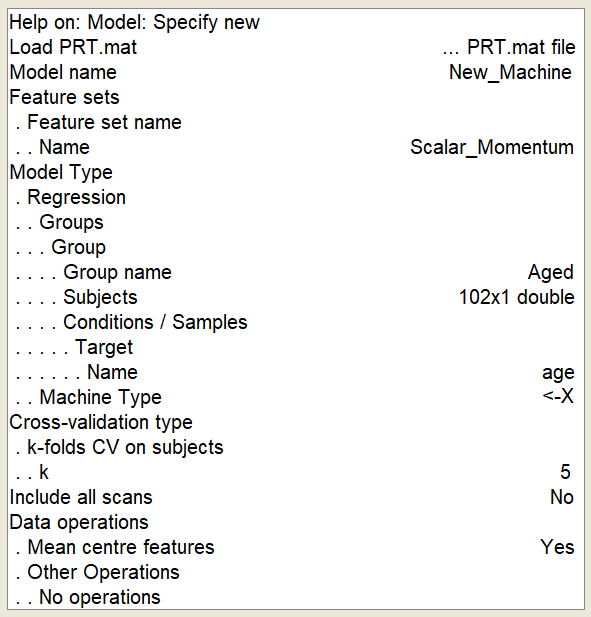
\includegraphics[scale=0.6]{new_machine_tutorial/new_machine_tutorial_model_specify_new_custom.png}
	\caption{`Model: Specify new' module.}
	\label{fig:new_machine_tutorial_model_specify_new_custom}
\end{figure}

\item Now we will describe how to fill the additional field that we skipped before, `Machine type'. Since KRR uses kernels, select the `Kernel machine' option, and, after that, in the `Kernel machine' field, select the `Custom machine' option. There are in total 3 fields here, 2 of which are new.

\begin{enumerate}

\item \textbf{Function:} You need to fill in the full path of your machine's file. In this particular case we have put the machine inside a folder named `new\_machine' so the full path would be something like `PRoNTo/machines/new\_machine/prt\_new\_machine.m'.

\item \textbf{Custom machine string arguments:} These are string parameters specific to each machine. They are usually required if the machine calls an external library for computations. These are the same string parameters mentioned in \ref{sssec:string_params}, so the reader is referred to this subsubsection for a further explanation. In our case, our custom machine requires no string arguments, so leave this field as it is.

\item \textbf{Custom machine optimization and parameters:} This is the same as the `Machine optimization and parameters' of the rest of the machines, with the only exception that no values are auto-filled. First select `Optimize hyper-parameter' and in the `Regularization hyper-parameter' insert the values $[0.01 0.1 1 10 100 1000]$. Finally change the `Cross-validation type for hyper-parameter optimization' to `k-folds CV on subjects' with k=4.

\bi
\item In case you do not want to do a nested cross-validation, you have to select the `No optimization', and in the `No optimization' field you should fill in any default parameter values that your machine requires. In our case that is the value of the $\lambda$ parameter, and is equal to 1. For further information regarding default parameter values the reader is referred to \ref{sssec:def_param_values}.
\ei

\end{enumerate}

\ei

The `Model: Specify new' module finally at this point should look similar to figure \ref{fig:new_machine_tutorial_model_specify_new_custom_final}.

\begin{figure}[!h]
	\centering
		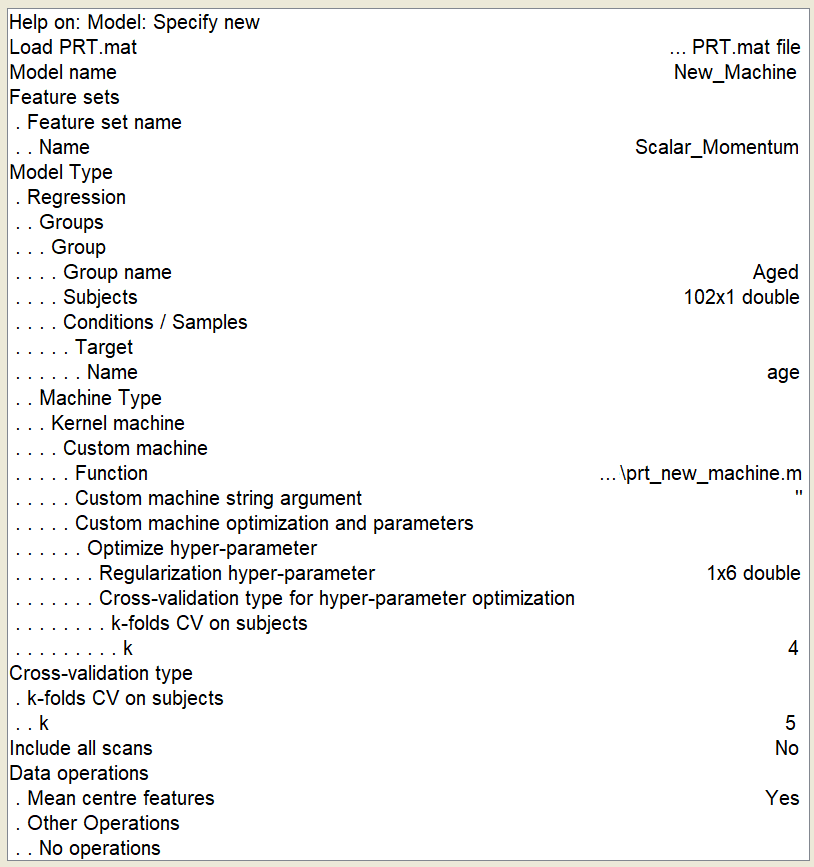
\includegraphics[scale=0.6]{new_machine_tutorial/new_machine_tutorial_model_specify_new_custom_final.png}
	\caption{Final configuration of the `Model: Specify new' module.}
	\label{fig:new_machine_tutorial_model_specify_new_custom_final}
\end{figure}



% \subsection{prt\_get\_machine.m}
% \lstinputlisting[firstline=87,lastline=102, firstnumber=87]{new_machine_tutorial/prt_get_machine.m}




% ===========================================================================


% ===========================================================================




\section{How to import your new machine in GUI}
\label{sec:new_machine_gui}

\subsection{prt\_defaults.m}

This is the script that sets most of the defaults used by PRoNTo. Each machine and/or library has its own parameters that might need to be set as defaults. You have to modify this script to include any default parameters your machine requires. There are 3 things you have to modify in this script.

\subsubsection{Machine lists for GUI}
\label{sssec:machine_lists}

Here we provide the GUI of PRoNTo with a list of names for each machine available. All names can be found inside \textbf{prt\_def.machine}. The names of the machines are grouped according to whether the machine is for classification or regression, whether it uses kernels or not, and whether it is a multi-kernel method or not. In our case since our toy method is KRR (named `New Machine'), which is for regression and uses kernels, we will need to add it to \textit{prt\_def.machine.reg\_K}.

\lstinputlisting[firstline=93,lastline=96, firstnumber=93]{new_machine_tutorial/prt_defaults.m}


\subsubsection{String parameters}
\label{sssec:string_params}

Some times machines require string arguments in their input, especially machine that are wrapper for libraries. Any string arguments your machine might require need to be defined here. Our toy machine (KRR) does not require any string arguments, so for an example we will present the string arguments required to run an L2-SVM as well as an $\epsilon$-SVR using the LIBSVM library.

\lstinputlisting[firstline=105,lastline=109, firstnumber=105]{new_machine_tutorial/prt_defaults.m}

If your machine required some string arguments to work, you would need to define the field \textit{prt\_def.model.new\_machine\_sargs} together with its proper string arguments. You should remember the name you give to this field (.new\_machine\_sargs) because you are going to use it later on.

\subsubsection{Default parameter values}
\label{sssec:def_param_values}

Besides string arguments, some machines may also require numeric values to be set as defaults. For example:

\lstinputlisting[firstline=128,lastline=133, firstnumber=128]{new_machine_tutorial/prt_defaults.m}

In this particular case, the default parameter values required by our toy machine (KRR) are the same as the LIBSVM and LIBLINEAR defaults shown above, so there is no need to add new ones explicitly. We are going to use this when asked in the next subsection. In case you need to specify new ones, you have to put it inside the \textit{prt\_def.model} structure. So your newly defined defaults would need to be inside a structure \textit{prt\_def.model.name\_args} where `name\_args' can be whatever name you want to give to your machine's arguments. You should remember this name because you are going to also use it later on.
\\

\noindent \textbf{Important Note:} The order with which the default parameter values will be harvested is the same as the one that are defined. So the user is advised to pay attention to that order since the machine will most likely not hit an error if run with transposed default parameter values.


\subsection{prt\_get\_machine\_ui.m}

This script is called when you use the GUI, to harvest the defaults you previously defined for each machine\footnote{\textit{prt\_get\_machine.m} is the equivalent of \textit{prt\_get\_machine\_ui.m} but for Batch. Modifications to \textit{prt\_get\_machine.m} will be discussed in the next section.}. You have to modify these scripts to properly harvest your machine’s defaults by including your machine in both of them. Be careful, however, because the GUI and the Batch have small differences in how they define things. Below is an example of how we defined our new machine, which is the same as KRR. First is an example from \textit{prt\_get\_machine\_ui.m}, and then from \textit{prt\_get\_machine.m}.

\lstinputlisting[firstline=110,lastline=122, firstnumber=110]{new_machine_tutorial/prt_get_machine_ui.m}

As we see in the code above, it is in this part that we are asking for the default parameter values that were defined in the previous section. If a new machine required different default parameter values, the user would have defined in the previous section, giving them a specific name, which would have been used in place of \textit{def.libsvmargs} in line \#113.


\subsection{prt\_ui\_copy\_model.m}

This is the script responsible for the GUI of the `Model: Specify from' module. Just as in \ref{sssec:machine_lists}, the user has to put the name of their machine here as well, in two instances, inside the if-loops \#970-1002 and \#1232-1296.

\subsubsection{First instance}

\lstinputlisting[firstline=993,lastline=1002, firstnumber=993]{new_machine_tutorial/prt_ui_copy_model.m}

\subsubsection{Second instance}

\lstinputlisting[firstline=1271,lastline=1291, firstnumber=1271]{new_machine_tutorial/prt_ui_copy_model.m}



\subsection{prt\_plot\_nested\_cv.m}

This script plots the results of the nested cv that appear on \textit{prt\_ui\_results}. The user has to modify the script, by including an extra case in the switch-loop of lines \#27-132, with their machine. Since our toy machine for this tutorial is KRR, we will be using logscale as well, and the x and y labels are also going to be the same.

\lstinputlisting[firstline=66,lastline=79, firstnumber=66]{new_machine_tutorial/prt_plot_nested_cv.m}



\subsection{prt\_weights\_*.m}

As mentioned in \ref{ssecc:outputs} in the note regarding weights, depending on your machine, in order for it to be able to visualize the contribution of different regions/features, some extra outputs might be mandatory. In general, in most cases weights are computed by \textit{prt\_weights\_linkernel.m}. So depending on your machine you might either use one of the existing  scripts, or you might need to create your own new \textit{prt\_weights\_*.m} for building the weights of your new custom machine. That, however, is depended on your machine so the user is advised to go through the existing \textit{prt\_weights\_*.m} scripts to further understand how they might need to structure theirs.


\subsection{Running your new machine}

If your machine's script is properly defined, and if everything was done accordingly, when you open the `Model: Specify new/from' modules, you are going to see your new custom machine as one of the options in the drop-down list like in figure \ref{fig:new_machine_tutorial_gui_model}.

\begin{figure}[!h]
	\centering
		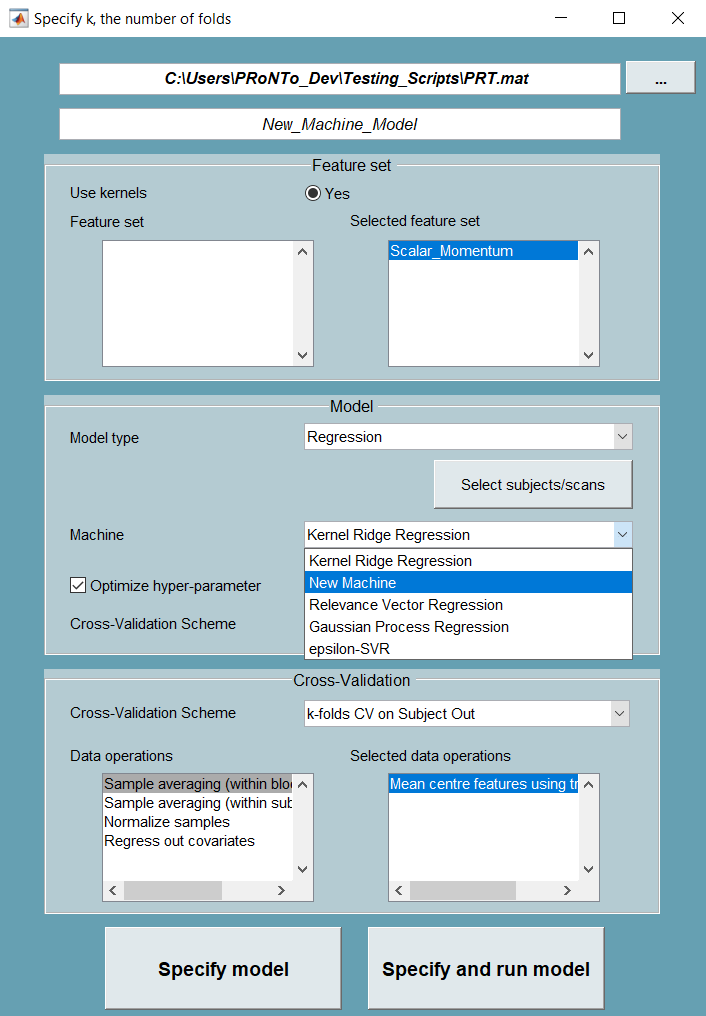
\includegraphics[scale=0.6]{new_machine_tutorial/new_machine_tutorial_gui_model.png}
	\caption{`Model: Specify new' module in GUI with the new machine option}
	\label{fig:new_machine_tutorial_gui_model}
\end{figure}





















	


%%%%%% ADVANCED TOPICS %%%%%%
%==========================================
\part{Advanced topics}
\label{sec:ADVTOP}
% % $Id: dev_guide.tex  $

\chapter{Developer's manual}
\minitoc

\section{Introduction}

As described in the Introduction, PRoNTo was developed using a modular structure. There are five main modules (`Data and Design', `Prepare Feature set', `Specify model', `Run model' and `Compute weights') and three reviewing and displaying modules (`Review data', `Review kernel and CV' and `Display results'). This structure not only facilitates the use of the toolbox but also new contributions from developers. These modules have very few dependencies between each other, and for most of them to work, one needs only to provide the `PRT.mat' obtained from the previous module and a few more module specific inputs. This means that the developer can contribute with code for any of the modules without having to adapt the whole toolbox to the changes.
\\

Developers can also work only on the module of interest and do not need to be familiar with the functions and sub functions that comprise the rest of the toolbox. In this chapter, we provide a brief description of how the code is organised and how one can contribute with new code, in particular new GUIs and Batch functions.
\\

After that, we provide instructions on how to integrate a new machine into PRoNTo. In the current version of PRoNTo, this is the most straightforward extension that can be added.
\\

And finally, we take an in-depth look into (1) the functions called at each step, (2) the PRT structure and its fields and (3) the files created at each step, as well as (4) the GUI and the batch behavior.


\section{Code organisation}

Although from the user's point of view there are five main modules, from the developer's side one can see PRoNTo's functions as belonging to three categories, depending on what they deal with (Figure \ref{Fig1.1}). The first set of functions and sub-functions is responsible for creating PRoNTo's GUIs and matlabbatch menu. The second set of functions comprise all the core routines that implement the machine learning methods (including extraction and preparation of the features, specification and estimation of a model, cross-validation, etc.). The last set of functions correspond to the actual machine learning algorithms that PRoNTo uses for classification and regression. We call these functions the `machines'. The main difference between this last set of functions and the rest, is that one does not need to be familiar with PRoNTo's PRT.mat structure or the rest of the code to be able to integrate a new machine. This can be done very easily, as shown below.

\begin{figure}[!htbp]
  \begin{center}
      
\includegraphics[height=2.2in]{images/code_pronto.png}
   \caption{Organisation of PRoNTo's functions. From the developer's perspective the code is organised in functions and sub functions that deal with the user interface experience (such as GUI and batch functions), the core functions that implement the machine learning approaches (including extracting and preparing the features, specification and estimation of a model, cross-validation routines, etc.) and the actual machine learning algorithms (also known as machines).}
    \label{Fig1.1}
  \end{center}
\end{figure}

\subsection{User interface}

The functions that deal with creating and running PRoNTo's main GUIs have the prefix `prt$\_$ui'. All GUI functions (`.m' files) have a corresponding `.fig' file. This file can be opened and edited using MATLAB's guide functionality. This way one can change the GUI and add extra options to the available menus (for more information, please consult MATLAB's documentation\footnote{http://www.mathworks.com/help/techdoc}).

PRoNTo's matlabbatch functions have either the prefix `prt$\_$cfg', to create a new menu on the batch interface and the prefix `prt$\_$run', to execute instructions using the variables from the corresponding `prt$\_$cfg' function. PRoNTo's batch functionalities work exactly like SPM. For more information on how to contribute with new matlabbatch functions please consult the developer's guide on the SPM8 manual\footnote{http://www.fil.ion.ucl.ac.uk/spm/doc/manual.pdf}.  

\subsection{Machine learning}

The machine learning routines comprise the core of PRoNTo. These routines do most of the necessary instructions to run all machine learning procedures currently implemented in the toolbox. They don't have a specific prefix but from the name of the .m file it is easy to find out what the function does (e.g. prt$\_$compute$\_$weights.m deals with creating new weights images). Most of the functions take as input the PRT.mat structure. Therefore, knowledge of this structure (see next chapter) is required in order to contribute with new code. In the future, we intend to make the process of introducing new feature selection algorithms and other model functionalities as easy as implementing a new machine, as described below.

\subsection{Machines}

Integrating a new machine algorithm, i.e. classifier or regressor, into the PRoNTo framework is straightforward. PRoNTo provides a function called `prt$\_$machine.m' that works as a wrapper around the different machine learning algorithms (functions with prefix `prt$\_$machine'). In brief, this wrapper translates PRoNTo's structure and internal variables into the required inputs for each machine. This way, the machine function needs only to read a simple input format that does not depend on knowledge of how PRoNTo works or of the PRT.mat fields (Figure \ref{Fig1.2}).

\begin{figure}[!htbp]
  \begin{center}
      
\includegraphics[height=3.0in]{images/machines.png}
   \caption{Code organisation for integrating a new machine with PRoNTo. `prt$\_$machine.m' works has a wrapper that translates PRoNTo's inputs into the machine format inputs and performs extensive error checks on these variables. The machines (such as `prt$\_$machine$\_$svm$\_$bin.m') perform the classifier/regression algorithms and have inputs and outputs that are not dependent on PRoNTo's internal structures.}
    \label{Fig1.2}
  \end{center}
\end{figure}

More specifically, to contribute with a new machine the developer needs to provide a matlab function, which reads the following input data structure, \textit{d}, and optional arguments, \textit{args}, (all fields are mandatory except where otherwise stated):

\begin{itemize}
\item \textit{d} - data structure with input to the classifier/regressor: \\
     \textit{.train} - training data (cell array of matrices of row vectors, each [Ntr x D]). Each matrix contains one representation of the data. This is useful for approaches such as multiple kernel learning. Ntr is the number of training examples and D is the dimension of the feature set (e.g. number of voxels).\\
     \textit{.test} - testing data  (cell array of matrices row vectors, each [Nte x D]). Nte is the number of testing examples and D the dimension of the feature set.\\
     \textit{.tr}$\_$targets - training labels (for classification) or values (for regression) (column vector, [Ntr x 1]).\\
     \textit{.use$\_$kernel} - flag: is data in form of kernel matrices (true) of in form of features (false)?
\item    \textit{args} (optional) - anything else that is specific to the algorithm (e.g. LIBSVM arguments).
\end{itemize}


\begin{figure}[!htbp]
  \begin{center}
      
\includegraphics[height=3.0in]{images/prtmachinesvmbin.png}
   \caption{`prt$\_$machine$\_$.m' function help. Example of a PRoNTo machine for 2-class SVM classification.}
    \label{Fig1.3}
  \end{center}
\end{figure}

In addition, the outputs of the function need to have the following format, so that they can be read by the wrapper and translated back to the PRoNTo framework (all fields are mandatory except where otherwise stated) (Figure \ref{Fig1.2}):

\begin{itemize}
\item \textit{output}  - output structure with fields:\\
\textit{.predictions} - predictions of classification or regression [Nte x D]. Nte is the number of test examples and D the dimension of the feature set.\\
\textit{.func$\_$val} (optional) - value of the decision function (if it applies).\\
\textit{.type}  (optional) - type of machine (string: `classifier' or `regressor').
\end{itemize}

The rest of the function can be designed entirely as the developer wishes. The last thing to have in mind is the name of the function itself. It needs to have the prefix `prt$\_$machine' (e.g. `prt$\_$machine$\_$svm$\_$bin' is a function that implements support vector machine binary classification by calling the LIBSVM library). Importantly, the cross-validation and performance measures are performed outside in the main PRoNTo framework, and therefore the machine function should provide only the necessary instructions to implement the classifier/regressor algorithm.
\\

Finally, the new machine is easily integrated with PRoNTo by including the name of the file in the corresponding GUI and Batch functions (prt$\_$ui$\_$model.m and prt$\_$cfg$\_$model.m, respectively).
\\

The same procedure applies to the weights functions. PRoNTo provides a wrapper function called `prt$\_$weights'. The procedure for integrating a new weights function is exactly the same as for a new machine.
\\

Both wrapper functions, `prt$\_$machine' and  `prt$\_$weights', perform extensive tests to make sure the machines and weights code complies to the specific inputs and outputs required by the framework.
\\


\section{PRoNTo folder structure}

PRoNTo contains several subfolders. 

\begin{itemize}
\item The folder \_devUtils and \_unitTests are for testing. The folder atlas contains AAL atlas and its labels, and a Brodmann atlas without labels. If developers want to add atlases, this folder is the first choice.
 
\item The batch folders contains all files for the batch module, which includes both the configuration (with `cfg' in the function names) and job execution (with `run' in the function names) functions. For each step in PRoNTo, we have cfg and run batch files implemented. Configuration functions generates the trees defining the interfaces of the modules in Batch. Job execution functions pass user inputs to lower functions in PRoNTo for calculations and estimations. GUI and batch share the same lower functions for computations and estimations. This modular design eases the development of new machines and functions in each module. 

\item The machine folder contains the different regression and classification algorithms. There are functions from libraries, `machines' ( with `prt\_machine' in the function names) which interface the libraries to PRoNTo, and functions computing weights for each machine.  If developers want to add a machine, they can open these functions and read their inputs and outputs. Some naming conventions are: `gp' for Gaussian processes, `cla' for classification, `krr' for kernel ridge regression. Names of these algorithms also refer to libraries, for example, `gp' refers to the `gpml' library, `MKL' refers to the `simpleMKL' library. Details on these are in ref{XXXX}.

\item The manual folder contains latex files for the manual, images and other contents. Developers can add to the documentation here.

\item The masks folder contains one first-level mask in the Data \& Design module until before version 3. This changed in PRoNTo v3.0 and more masks (in nifti format) can be added.

\item In utils folder, there are several lower level functions e.g. checking if inputs are alpha numeric, or performing some operations on the kernels, such as split data in the kernel and normalise kernels. 
 
\item Beyond the above mentioned subfolders, functions with `ui' in their names define the GUI interfaces, i.e. *\_ui\_*.fig and *\_ui\_*.m file pairs define the figure and how the GUI behaves, respectively. We used GUIDE to create GUI and add custom functions and codes to extend these interface functions. 
 
\item The rest of the `prt\_' functions perform the computations and estimations defined in each module. 

\end{itemize}

%======================================================================



%======================================================================

\section{Data \& Design}

\subsection{PRT fields created}

PRT structure is created after specifying this module. More specifically, two fields of PRT.mat are filled: group and masks. Users input all their data, experimental design (e.g., modalities, runs, conditions) and other related information here (e.g. covariates, regression values). After this step, data information is stored in the group field of PRT.mat and nifti 1st level masks are stored in the masks field of PRT.mat.  HRF overlap and delay parameters are stored in masks field too. Below is a list of subfields in \textcolor{blue}{PRT.group} and \textcolor{blue}{PRT.masks}:

\begin{itemize}
\item \textcolor{blue}{PRT.group}

\begin{itemize}
\item \textcolor{blue}{PRT.group.gr\_name}: Storing group names
\item \textcolor{blue}{PRT.group.subject}: Storing subject information

\begin{itemize}
\item \textcolor{blue}{PRT.group.subject.subj\_name}: Storing subject names
\item \textcolor{blue}{PRT.group.subject.modality}: Subfields containing information on regression targets, covariates, modality name, design and scans. Note: classification labels are specified in Specify model module later.


\end{itemize}
\end{itemize}

\item \textcolor{blue}{PRT.masks}

\begin{itemize}
\item \textcolor{blue}{PRT.masks.mod\_name}: Name of corresponding modality
\item \textcolor{blue}{PRT.masks.type}: Type of the data
\item \textcolor{blue}{PRT.masks.fname}: The full path of the specified mask
\item \textcolor{blue}{PRT.masks.hrfoverlap}: Storing information on HRF overlap (default: 0)
\item \textcolor{blue}{PRT.masks.hrfdelay}: Storing information on HRF delay (default: 0)

\end{itemize}
\end{itemize}


%----------------------------------------------------------------------

\subsection{Files created}

PRT structure, saved in a PRT.mat file in the path specified by the user.


%----------------------------------------------------------------------

\subsection{GUI behaviour}

GUI of Data \& Design module provides interfaces for users to specify where to store the PRT structure and files, data information, experimental design, masks and all other related information.

\begin{itemize}
\item Save button creates PRT structure.
\item Load button loads previously created PRT.mat and checks its compatibility.
\item Review button provides a graphical review of all the input information and the interface for modifying some HRF parameters.
\end{itemize}
 
%----------------------------------------------------------------------

\subsection{Batch behaviour}

The Batch of Data \& Design module provides users similar functions and interfaces as GUI. However, there are some differences.

\begin{itemize}
    \item One is that the batch job can be saved as a .mat file or a .m function. Both users and developers can make changes directly in these files.
    \item Another difference is that both users and developers should be careful about the names of modalities when using the Batch. The names shall be consistent.
    \item One more difference is that HRF delay and overlap can be changed directly in the Batch of Data \& Design. In GUI, they can be modified in Review.
\end{itemize}

%----------------------------------------------------------------------

\subsection{Functions called}


\textbf{\underline{GUI:}}

\begin{enumerate}

\item \textcolor{red}{prt\_ui\_design.m} and \textcolor{red}{prt\_ui\_design.fig}

The functions define GUI interfaces and the figure for Data \& Design module. It initializes the code, executes each button press in this module in GUI, checks if the inputs are correct and creates output in MATLAB prompt. If developers want to make changes in this GUI module (e.g., a button’s or menu’s functions), you’ll find subfunctions with corresponding names in \textcolor{red}{prt\_ui\_design.m} and add codes there. % are sub-functions with illustrations pointing you which code segments define which button press.
Some important functions called by \textcolor{red}{prt\_ui\_design.m} are summarized as follows.

% Sub-functions include:
\begin{itemize}
\item \textcolor{red}{prt\_data\_modality.m} and \textcolor{red}{prt\_data\_modality.fig}

The two files define the GUI panel for specifying the information of the modality, experimental design, covariates and regression targets. The \textcolor{red}{prt\_data\_modality.m}  also calls:

\begin{itemize}
\item \textcolor{red}{prt\_data\_conditions.m} and \textcolor{red}{prt\_data\_conditions.fig}, for receiving inputs for conditions, i.e. experimental design.
\item \textcolor{red}{prt\_check\_design.m}, for checking the design and discards scans according to overlapping conditions or the minimum time interval between conditions based on the HRF function and specified HRF parameters.
\end{itemize}

\item \textcolor{red}{prt\_get\_defaults.m} and \textcolor{red}{prt\_defaults.m}

Default settings of PRoNTo are stored in \textcolor{red}{prt\_defaults.m}, including global defaults such as colour, parameters for the data and design, preprocessing, default atlas for ROI definition, arguments of different machines, and parallelization of the code. The function \textcolor{red}{prt\_get\_defaults.m} gets the relevant default values from \textcolor{red}{prt\_defaults.m} for this module. For instance, the code `color=\textcolor{red}{prt\_get\_defaults}(`color')' sets colors of backgrounds and figure parameters for Data \& Design module.

\item \textcolor{red}{prt\_data\_review.m} and \textcolor{red}{prt\_data\_review.fig}

The two functions define the GUI for reviewing the data.

\end{itemize}

\item \textcolor{red}{prt\_load.m} and \textcolor{red}{prt\_struct.m}

This function is called by \textcolor{red}{prt\_ui\_design.m}. When clicking the load button, the functions are called to load PRT.mat and check the fields in it for backwards compatibility. If you add a field somewhere in the PRT and that field is necessary for display or further analyses, the prt\_struct file should be amended to set default values for that field to ensure that older PRT files can still be read and modified.

\end{enumerate}

\noindent \textbf{\underline{Batch:}}

\begin{enumerate}
    \setcounter{enumi}{2}

\item \textcolor{red}{prt\_cfg\_design.m} and \textcolor{red}{prt\_run\_design.m}

\begin{itemize}
\item Function \textcolor{red}{prt\_cfg\_design.m} is the Data \& Design module configuration file and builds the PRT.mat data and design structure.
\item Function \textcolor{red}{prt\_run\_design.m} is the job execution function, which takes a harvested job data, rearranges them into PRT structure and saves it.
\end{itemize}

\end{enumerate}

At this stage, the GUI and batch have very little code in common. Hence, changes in the GUI have to be performed independently in the batch and conversely.  


%======================================================================



%======================================================================

\section{Prepare feature set}

\subsection{PRT fields created}

There are two fields created in PRT.mat in this step, too. Field \textit{fs} (feature set) and \textit{fas} (file array structure). The information for the two fields is specified by users in the `Specify modality to include' panel.

For each modality, a file array is created containing the data (detrended if specified) from the selected modality. The field \textcolor{blue}{PRT.fas} is linked to this file array. In \textit{fas}, the information stored refers to the modality (as defined in Data \& Design). This means that multiple MRI sessions, entered as different runs will each create a \textit{fas}. A \textit{fas} links to a \textit{.dat} file with dimensions of \#images x \#features within the first-level mask and stores feature operations (detrend and detrend parameters), header of the first image for recovering images if needed, and indices of all features within the first-level mask.
\\

The field \textit{fs} refers to the kernel/feature set that is created. It is a structure of size number of feature sets created by the user. Within \textit{fs}, there is information on feature set name, kernel file, ID matrix, information of using multiple kernels. This field also contains information about the second-level mask and/or the atlas (used to build the kernel).
\\

One important subfield is the ID matrix, which contains information about the modalities selected in the feature set arranged in six different columns: group, subject, modality, condition, block and scan.

\begin{itemize}
\item The name of the columns are stored in \textcolor{blue}{PRT.fs.id\_col\_names}.
\item The group numbers, subject numbers, modality labels, condition numbers, block labels and scan numbers themselves are stored in \textcolor{blue}{PRT.fs.id\_mat}, whose dimension is the number of samples x 6.
\end{itemize}

The ID matrix is referred to in the `Review kernel \& CV' reviewing tool in PRoNTo, where a graphical display shows the structure of this matrix.

\begin{itemize}
\item In addition, there is a \textit{fas} subfield in \textcolor{blue}{PRT.fs}, that is different from \textcolor{blue}{PRT.fas}. This subfield in \textit{fs} refers to the modality and scan indices of the feature set modalities in the \textit{fas} structure. It is useful when modalities are concatenated in samples (e.g. accessing the correct scans from multiple runs in an MRI experiment, with each run linked to a different \textcolor{blue}{PRT.fas} file array).

\end{itemize} 

% \begin{itemize}
% \item \textcolor{blue}{PRT.fs}

% \begin{itemize}
% \item \textcolor{blue}{PRT.fs.fs\_name} - 
% \item \textcolor{blue}{PRT.fs.k\_file} - 
% \item \textcolor{blue}{PRT.fs.id\_col\_name} - 
% \item \textcolor{blue}{PRT.fs.} - 
% \item \textcolor{blue}{PRT.fs} - 
% \item \textcolor{blue}{PRT.fs} - 
% \item \textcolor{blue}{PRT.fs} - 


% \end{itemize}

% \item \textcolor{blue}{PRT.masks}

% \end{itemize}


%----------------------------------------------------------------------

\subsection{Files created}

\begin{itemize}
\item FAS .dat file.
\item A kernel matrix (.mat with variable Phi, a cell array with a kernel in each cell).
\item Updated masks and/or atlases (nifti resampled at the size of the input data images).
\end{itemize}


%----------------------------------------------------------------------

\subsection{GUI behaviour}

The GUI of `Prepare feature set' takes the PRT.mat created in Data \& Design module and provides interfaces for users to further specify feature sets, their names, selected modalities, operations on feature sets and the atlas for defining kernels. 


%----------------------------------------------------------------------

\subsection{Batch behaviour}

The module of `Prepare feature set' in the Batch is similar to the GUI. However, the batch requires consistent names across modules. Running important modules altogether will overwrite the PRT.mat, hence delete the links between the PRT.mat and the computed feature set(s) and kernel(s). \textit{FAS} will be recreated each time the Batch is launched. More detailed illustrations on this please refer to \ref{sec:matlabbatch_3_4}.


%----------------------------------------------------------------------

\subsection{Functions called}

\textbf{\underline{Core:}}

\begin{enumerate}

\item \textcolor{red}{prt\_fs.m}

Gather information on the modalities to build file arrays containing the (detrended) data and computes the linear kernels. It resizes the second-level masks and atlas if needed. \textcolor{red}{prt\_fs.m} calls:
\begin{itemize}
\item \textcolor{red}{prt\_init\_fs.m} to populate basic fields in \textcolor{blue}{prt.fs}, like the file array structure, kernel data structure and feature set parameters. 
\item \textcolor{red}{prt\_fs\_modality.m} to write the kernel matrix to the user-defined path as well as the feature set if needed.
\end{itemize}

\item \textcolor{red}{prt\_init\_fs.m}

     This function initialises the next function (\textcolor{red}{prt\_fs\_modality.m})
     
\item \textcolor{red}{prt\_fs\_modality.m}

    For each selected modality, builds and reads from the file array to compute the kernel. It calls \textcolor{red}{prt\_get\_defaults.m} to get defaults about fs, and \textcolor{red}{prt\_load\_blocks.m} to access one or more blocks of data to avoid memory overload. 

\end{enumerate}


\noindent \textbf{\underline{GUI:}}

\begin{enumerate}
\setcounter{enumi}{3}

\item \textcolor{red}{prt\_ui\_prepare\_data.fig} and \textcolor{red}{prt\_ui\_prepare\_data.m}

GUI to specify how many feature sets will be used in the feature set. In v2, these modalities can either be concatenated (e.g. multiple runs of an experiment), or used in multiple kernel settings (e.g. sMRI grey and white matter). For each modality entered, the function calls \textcolor{red}{prt\_ui\_prepare\_datamod.m} to specify parameters for this specific modality.

\begin{itemize}
\item \textcolor{red}{prt\_ui\_prepare\_datamod.fig} and \textcolor{red}{prt\_ui\_prepare\_datamod.m}

Functions \textcolor{red}{prt\_ui\_prepare\_datamod.m} and \textcolor{red}{prt\_ui\_prepare\_datamod.fig} are called by \textcolor{red}{prt\_ui\_prepare\_data.m} to accept user inputs about modalities, to compute the file array and for building the kernel.
\end{itemize}

\end{enumerate}

\noindent \textbf{\underline{Batch:}}

\begin{enumerate}
\setcounter{enumi}{4}

\item \textcolor{red}{prt\_cfg\_fs.m} and \textcolor{red}{prt\_run\_fs.m}

The fs configuration file constructs the feature set for each modality. The related job execution function harvests all inputs passed by \textcolor{red}{prt\_cfg\_fs.m} and arrange them into the PRoNTo structure. It calls \textcolor{red}{prt\_fs.m} to build file arrays and compute kernels from them.


\end{enumerate}




%======================================================================



%======================================================================

\section{Specify model}

Specify model module computes the inputs for the models, but does not estimate/run the models. Main inputs for this module are feature sets, where users select which feature set will be used to build the model, model type (regression or classification), selection of samples and classes, machines, cross validation (CV) strategy and data operations.

\subsection{PRT fields created}

Two subfields in \textcolor{blue}{PRT.model} are created and filled: \textcolor{blue}{PRT.model.model\_name}, which stores the name of the model and \textcolor{blue}{PRT.model.input} which stores all the other information. Another subfield \textcolor{blue}{PRT.model.output} is only created but is not filled here. It will be filled after the model is estimated (Run model module). Below is an illustration of the information stored in \textcolor{blue}{PRT.model.input}:
 
\begin{itemize}
 
\item \textcolor{blue}{PRT.model.input.use\_kernel}: 1 (use kernel methods). From version 3 there is also option 0 (non-kernel methods).

\item \textcolor{blue}{PRT.model.input.type}: Regression or classification. This field is being visited very often within PRoNTo.

\item \textcolor{blue}{PRT.model.input.machine}: Stores information of the chosen machine. The algorithms can be found in the subfolder \textit{PRoNTo/machines/}.

\item \textcolor{blue}{PRT.model.input.use\_nested\_cv}: Whether to optimize hyperparameters (1) or not (0).

\item \textcolor{blue}{PRT.model.input.nested\_param}: A vector of user-defined parameters if \textcolor{blue}{PRT.model.input.use\_nested\_cv} is 1. This can also be empty, which means to leave it for the algorithm to set values by default. The default values are specified in \textcolor{blue}{PRT\_nested\_CV} at the `Run model' step.

\item \textcolor{blue}{PRT.model.input.cv\_type\_nested}: The CV strategy for the inner CV loop.

\item \textcolor{blue}{PRT.model.input.cv\_k\_nested}: Value of k for the k-fold inner CV loop. If 10 is here, it means that the strategy takes 90\% of the data for training, and 10\% of the data for test.
\begin{itemize}
\item Leave-one-out has k=0.
\end{itemize}

\item \textcolor{blue}{PRT.model.input.subsample}: 

\item \textcolor{blue}{PRT.model.input.indmodels}:

\item \textcolor{blue}{PRT.model.input.class}: Contains the user-specified selection for each class. 

\begin{itemize}
\item It's a structure of size number of classes (classification) or 1 (regression). It specifies the groups, subjects within that group and conditions for each class, with a similar structure as in \textcolor{blue}{PRT.group} (without the modalities). And we identify which indices in the global ID matrix are selected to build the specified class.
\item The CV matrix and everything else are built from here. This can be viewed in Review kernel \& CV. Note: it’s always good to have a check on the CV matrix to ensure the inputs do what you want. You can also make a CV matrix yourself and input via Custom choice in Cross-validation scheme. In the Review module, you can view the classes specified.
\end{itemize}


\item \textcolor{blue}{PRT.model.input.samp\_idx}: Index of the selected samples for this model, in the corresponding feature set.

\item \textcolor{blue}{PRT.model.input.include\_allscans}:


\item \textcolor{blue}{PRT.model.input.targets}: Prediction targets for building the model.

\item \textcolor{blue}{PRT.model.input.targ\_allscans}:

\item \textcolor{blue}{PRT.model.input.covar}:

\item \textcolor{blue}{PRT.model.input.cov\_allscans}:

\item \textcolor{blue}{PRT.model.input.cv\_k}: Value of k for the k-fold outer CV loop (i.e. the main or external CV).

\item \textcolor{blue}{PRT.model.input.cv\_mat}: CV matrix for the external CV.

\item \textcolor{blue}{PRT.model.input.cv\_type}: CV type for the external CV.

\item \textcolor{blue}{PRT.model.input.operations}: Stores user selected data/kernel operations as an integer vector. The operations will be applied according to this order. 
 
\end{itemize} 

Specify model module creates and estimates inputs for estimating the model. It is easy to script. For example, higher-level users and developers can copy \textcolor{blue}{PRT.model} and change any of the sub-fields listed above when it is needed manually. CV matrix is computed based on CV schemes specified by the user.

%----------------------------------------------------------------------

\subsection{Files created}

No new files are created at this stage.


%----------------------------------------------------------------------

\subsection{GUI behaviour}

In GUI, users can choose Specify model alone or Specify and run model. It computes the sample indices based on the classes, computes CV matrix based on the ID matrix (and labels in case of `Leave-per-Group-Out') and CV specifications, and it gathers the targets and covariates based on the class definition. ID matrix is used here as a reference to obtain these sub-groups of indices, targets and covariates for building the particular model. CV matrix can also be input by users via Custom CV.


%----------------------------------------------------------------------

\subsection{Batch behaviour}

Batch provides similar functions to GUI, but the Specify model and Run model modules are separated.

%----------------------------------------------------------------------

\subsection{Functions called}

\textbf{\underline{Core:}}

\begin{enumerate}

\item \textcolor{red}{prt\_model.m}

This function initialises the model data structure (by calling \textcolor{red}{prt\_init\_model.m}), computes targets and the sample index.

\begin{itemize}
\item In PRoNTo v2.1, classification and regression are addressed differently. In classification, the codes visit information stored in the design. For regression, only subject-level analysis is available, so the codes do not go into the design.
The sub-functions compute\_targets and compute\_target\_reg inside \textcolor{red}{prt\_model.m} compute the prediction targets for classification and regression, respectively. Targets that are not selected for this model are put to zeros. From PRoNTo v3.0 both classification and regression compute the prediction targets using an updated version of the compute\_targets sub-function.
\end{itemize}
 
\item One note is that the labels of different classes are 1,2,3,..., here referring to Class 1, Class 2, Class 3, ... respectively. They will be converted to class labels accepted by the actual machines inside the machine function, if needed. For example, if Faces and Houses are selected by the user as Class 1 and Class 2, respectively, and if we use SVM, the labels 1 and 2 will be converted to -1 and 1 in the machine \textcolor{red}{prt\_machine\_svm\_bin.m}.

\item \textcolor{red}{prt\_compute\_cv\_mat.m}

It computes the CV matrix. Inner and external CV loops call the same function. This function is accessed in the Specify model and Run model modules. In PRoNTo, CV schemes are shown in abbreviations, for example:

\begin{itemize}
\item LOSO: leave-one-subject-out. If we have 56 subjects, and 10 folds. Then 5 subjects in each fold, the remaining 6 will be distributed to the first 6 folds. As a result, 6 subjects in the 1 to 6 folds, 5 subjects in the remaining 4 folds. The reason to do this is for distributing subjects more evenly.
\item LORO:leave-one-run-out. There is no leave-multiple-run-out option in PRoNTo, only leave-one-run-out.
\end{itemize}

Other CV schemes can be found in the user manual. PRoNTo also provides interfaces for users to input their own CV design, i.e. the custom CV. Users can input their own CV matrix via this interface. The codes for this part here only check things. Relevant codes of the interface do the real work. Please note that nested CV  will not be computed in Specify model step, but during the model estimation.
 
\end{enumerate}


\noindent \textbf{\underline{GUI:}}



\begin{enumerate}
\setcounter{enumi}{2}

\item \textcolor{red}{prt\_ui\_model.m}  and \textcolor{red}{prt\_ui\_model.fig}

The GUI functions that define the interfaces of Specify model module. It calls several other functions among which:

\begin{itemize}
\item \textcolor{red}{prt\_ui\_select\_class.m} and \textcolor{red}{prt\_ui\_select\_class.fig}

This function provide interfaces to users to select classes for classification problems.


\item \textcolor{red}{prt\_ui\_select\_reg.m} and \textcolor{red}{prt\_ui\_select\_reg.fig}

This function provide interfaces to users to select data for regression analysis in regression problems.

\item \textcolor{red}{prt\_ui\_specify\_CV\_basis.m} and \textcolor{red}{prt\_ui\_specify\_CV\_basis.fig}

This function provides interfaces for users to input their custom CV information. It calls \textcolor{red}{prt\_ui\_custom\_CV.m} and \textcolor{red}{prt\_ui\_custom\_CV.fig} to allow custom CV specification.

\item \textcolor{red}{prt\_model.m}

This function configures and builds the \textcolor{blue}{prt.model} structure.

\item \textcolor{red}{prt\_cv\_model.m}

This function runs a CV on a given model.

\end{itemize}


\end{enumerate}


\noindent \textbf{\underline{Batch:}}


\begin{enumerate}
\setcounter{enumi}{6}

\item \textcolor{red}{prt\_cfg\_model.m} and \textcolor{red}{prt\_run\_model.m}

Functions define the tree and behaviors of the Specify model module in the Batch.


\end{enumerate}




%======================================================================



%======================================================================

\section{Run model}

Specify model sets up the configuration of the model. Run model module performs the training and testing. It includes hyperparameter optimization by using inner cross-validation (CV) schemes, model training and testing using external CV schemes, computing statistics for model performance measures and PRT.mat updates. The machine is called in this module for model evaluation. In GUI, this module can be run directly from Specify model. In Batch, it is separated from the Specify module.
\\

\noindent \textbf{\underline{How is the cross-validation implemented?}}
\\

CV schemes are important to model training and testing. In PRoNTo, this is mainly performed by \textcolor{red}{prt\_cv\_model.m}. After some initialization steps, it begins the main CV loops, i.e. external CV loops. If the user chooses to optimize hyperparameters, each fold from the external CV is sent to inner CV schemes. Users can choose different CV strategies for inner and external CV. The function \textcolor{red}{prt\_nested\_cv.m} is called to optimize hyperparameters. The best hyperparameter is returned to \textcolor{red}{prt\_cv\_model.m} within each external fold. Whether hyperparameter is optimized or not, one model is estimated per fold by calling \textcolor{red}{prt\_cv\_fold.m}. This is followed by statistic computations for model performance measures, by calling \textcolor{red}{prt\_stats.m}. In \textcolor{red}{prt\_cv\_model.m}, statistics are calculated and stored at fold level and model level. Model level statistical metrics are obtained by concatenating results across folds in version 2. This changed to averaging metrics across folds in version 3. PRT.mat is updated and saved in the end of \textcolor{red}{prt\_cv\_model.m}.
\\[2cm]

\noindent \textbf{\underline{How is the parameter optimization implemented?}}
\\

In many situations, it is preferable to optimize hyperparameters to increase the predictive model performance. If users choose this step, each external fold is sent to \textcolor{red}{prt\_nested\_cv.m} and goes through an inner CV loop. The training data in this external fold is splitted into training and testing sets inside \textcolor{red}{prt\_nested\_cv.m} according to the inner CV schemes. Before looping over inner CV folds, \textcolor{red}{prt\_nested\_cv.m} checks user-defined hyperpameter ranges. Default ranges are used if there are no user inputs. Hence, this function first loops over each hyperparameters and then loops over inner folds for each hyperparameter. It calls \textcolor{red}{prt\_cv\_fold.m} to perform the model training and testing. One model is created for each inner fold, generating predictions. Within every loop of a certain hyperparameter, model performance metrics are calculated for each inner fold.
\\

Statistic calculation is done by calling \textcolor{red}{prt\_stats.m}. In version 2, we concatenate predictions from each inner fold to obtain the model-level performance measures. Specifically, balanced accuracy is used for classification and MSE is used for regression. This generates one metric value per hyperparameter. After completing the inner CV for all values of the hyperparameter, we choose the best one according to the metrics, i.e. the hyperparameter generating the maximum balanced accuracy is selected as the best one for classification and the hyperparameter generating the minimum MSE is selected as the best one for regression. \textcolor{red}{prt\_nested\_cv.m} returns the best hyperparameter to \textcolor{red}{prt\_cv\_model.m} for the outer model training and testing.
\\

\noindent \textbf{\underline{How are the machines organized?}}
\\

Model training and testing for both external and inner CV are done by calling \textcolor{red}{prt\_cv\_fold.m}. This function configures model parameters and applies user-specified data operations before feeding them to the machines. It calls \textcolor{red}{prt\_machine.m} which will then distribute to the specific machine A structure containing data information related to CV folds and information of the selected machine are passed to \textcolor{red}{prt\_machine.m}. After some input checks, \textcolor{red}{prt\_machine.m} passes these information to the specific machine function. The machine-specific functions are in the machine folder, with ‘machine’ in their names. Some of them are wrapper functions of the core functions in several third-party libraries, such as Libsvm, Liblinear and SimpleMKL.
\\

PRoNTo uses wrapper functions to organise inputs (data, class labels, targets, function arguments and hyperparameters) to formats accepted by actual machines in those libraries, and organise outputs from these machines to PRoNTo accepted formats. For instance, \textcolor{red}{prt\_machine\_svm\_bin.m} is a wrapper of binary SVM in Libsvm. PRoNTo takes the hyperparameter range from GUI or Batch, then combines it with other machine arguments required by Libsvm. Training and testing datasets are organised according to Libsvm conventions. Predictions and model parameters from the binary SVM machine are stored according to PRoNTo conventions. Machine arguments include options provided by third-party libraries and hyperparameters (e.g. C for SVM). Most of the type, we define machine options in \textcolor{red}{prt\_defaults.m}.
\\
 
\noindent \textbf{\underline{What are the input and output for a machine?}}
\\

Generally speaking, each \textcolor{red}{prt\_machine\_*.m} function accepts two inputs, a structure d containing the data information and a structure args containing machine-specific information including options and hyperparameter values. In structure d: d.train and d.test contain the training and testing data respectively. The d.tr\_targets refers to targets of the training data. There is no need to pass d.te\_targets as model performance is evaluated outside of the machine, in PRoNTo \textcolor{red}{prt\_stats.m}. One flag d.use\_kernel contains information about whether the machine is a kernel machine or not.. In version 2, this is by default always true. The output of each machine contains prediction values, function values from the decision function, model parameters and the type of the machine (classifier or regression). 
% \\[2cm]


%----------------------------------------------------------------------


\subsection{PRT fields created}

Two new fields are created in PRT.mat in this module: \textcolor{blue}{PRT.model.output.fold}, \textcolor{blue}{PRT.model.output.stats}. In \textcolor{blue}{PRT.model.output.fold}, several subfields are generated to store information of hyperparameter effects, prediction values in each fold, fold-level statistics, decision function values, model parameters and other information specific to some machines (e.g. kernel contributions for MKL models).

%----------------------------------------------------------------------

\subsection{Functions called}

\textbf{\underline{Core:}}

\begin{enumerate}

\item \textcolor{red}{prt\_cv\_model.m}, \textcolor{red}{prt\_nested\_cv.m} and \textcolor{red}{prt\_cv\_fold.m}

This function is where CV schemes are implemented within PRoNTo. Before looping over CV folds, it gets the model index, configure variables based on the CV matrix, gets values and variables for model estimation, such as user-specified targets, class numbers, kernels, and machine arguments. It also initializes outputs. This function calls \textcolor{red}{prt\_nested\_cv.m} to optimize hyperparameters. It calls \textcolor{red}{prt\_cv\_fold.m} to train and test the predictive models. \textcolor{red}{prt\_nested\_cv.m} also calls \textcolor{red}{prt\_cv\_fold.m} within each inner fold to estimate models. 
       
\item \textcolor{red}{prt\_stats.m}

This function is called by \textcolor{red}{prt\_cv\_model.m} to calculate fold-level and model-level metrics measuring the model performance. It takes predictions, model type, test targets, and class numbers as inputs.  For classification, confusion matrix, accuracy, balanced accuracy, class accuracy and predictive value are calculated.  For regression, MSE (and normalized MSE), correlation and squared correlation are calculated. These metric values are passed as outputs in a `stats' structure.
       
\item \textcolor{red}{prt\_machine.m} and \textcolor{red}{prt\_machine\_*.m} functions

These functions are in the machine folder carrying out the actual modeling. \textcolor{red}{prt\_machine.m} is called by \textcolor{red}{prt\_cv\_fold.m} and passes data information and machine arguments to the machine-specific functions \textcolor{red}{prt\_machine\_*.m}, which are generally wrapper functions of the core machines provided by several third-party libraries. These wrapper functions perform some initial checks on the inputs, re-structure data and arguments to formats accepted by the core machines, then checks outputs from the estimated models and organize them into PRoNTo accepted structures. 

\end{enumerate}


\noindent \textbf{\underline{GUI:}}

\begin{enumerate}
\setcounter{enumi}{3}

\item \textcolor{red}{prt\_ui\_model.m} calls \textcolor{red}{prt\_cv\_model.m} to start Run model module if the user clicks `Specify and Run'.

\item \textcolor{red}{prt\_ui\_cv\_model.m} and \textcolor{red}{prt\_ui\_cv\_model.fig}

These are functions implementing the GUI interface for Run model. It loads the specified models from the PRT and fills a list that the user can select from. \textcolor{red}{prt\_cv\_model.m} is called sequentially on the models selected for estimation.

\end{enumerate}

\noindent \textbf{\underline{Batch:}}

\begin{enumerate}
\setcounter{enumi}{5}

\item \textcolor{red}{prt\_cfg\_cv\_model.m} and \textcolor{red}{prt\_run\_cv\_model.m}

These are the batch functions defining the trees of the Run Model module and execute the configurations. It accepts inputs from \textcolor{red}{prt\_cfg\_model.m}, organise them into proper structures. From version 2 and on, permutation test is interfaced in Batch in this module.

\end{enumerate}


%======================================================================



%======================================================================

\section{Compute weights}


Two steps are used to compute weights, that are carried out by prt\_compute\_weights.m and prt\_weights\_*.m for specific machines. Weight maps can be built as voxel-wise images or ROI-wise images. For multiple kernel learning, maps indicating kernel contributions with ranking information can be obtained.
\\

\noindent \underline{\textbf{How are the weights computed in PRoNTo?}}
\\
 
The function \textcolor{red}{prt\_compute\_weights.m} accepts information from \textcolor{red}{PRT.m} and some user-defined information, such as which model the weight image is for, where to save, flags indicating whether to build weights for each permutation (batch only) and/or for each ROI, and atlas for ROI-wise weight image if it is selected by the users. If different modalities were used without concatenating the samples, one weight map is built for each modality.
\\
 
For each modality, weight computation is classified into classification and regression problems. One weight image will be built per class for multi-class problems, while only one weight map is built for binary classification or regression problems. These are implemented in \textcolor{red}{prt\_compute\_weights\_class.m} and \textcolor{red}{prt\_compute\_weights\_regre.m}, respectively. Processing routines for classification and regression are similar to each other. Take classification as an example to illustrate the routine. The code finds the type of data (nifti or MEEG) and machine first, then creates image names. One tricky part is the multiple indexing step. Getting the correct indices from the file array (.dat file), feature sets and each slice along z axis within ROIs is implemented here. In Prepare feature set module, we need a subset of images to build the file array, from which we use potentially a subset to build a kernel. In order to build the weight image, we therefore need to access indices from both file arrays and feature sets fs structures. To not to overload the memory, we build the weight image slice by slice along the z axis, since most images are 3-D files. So we need to take indices from that slice, within both the second-level and the first-level masks. The three levels of indices are necessary to build weight maps.
\\
 
The next step is to create maps. If the user selects to build weight images for each permutation, relevant checks and codes are in \textcolor{red}{prt\_compute\_weights.class.m}. Image initialization is performed before the weight computation. During weight computation, we access indices within the 2nd level mask along the z axis. For weight maps using the whole brain, we use similar approaches with slightly different inputs. In \textcolor{red}{prt\_compute\_weights.m}, the variable flag2 tells if we want to get one weight per region instead of one weight per voxel, so weight computation will be changed according to this. We build one image for each fold, which results in a 4-D image where the last map is an average over all folds. Data operations are applied. If MKL is used, codes get Beta here. Following procedures are to build the weights, reshape them into the correct dimensions, normalize the weights for visualization and save the images.
\\
 
The code performing actual multiplication for weights is done by using \textcolor{red}{prt\_weights.m} in the machine folder within \textcolor{red}{prt\_compute\_weights\_class.m} and \textcolor{red}{prt\_compute\_weights\_regre.m}. This function calls other \textcolor{red}{prt\_weights\_*.m} in the machine folder. Since different machines have different formulations, computing weights using outputs from these machines may vary too. Take \textcolor{red}{prt\_weights\_sMKL\_cla.m} as an example: the inputs are structure d and args similar to inputs to machines. But the data loaded in \textcolor{red}{prt\_compute\_weights\_class.m} and \textcolor{red}{prt\_compute\_weights\_regre.m} is d.datamat. By taking coefficients from d.coeffs and data from d.datamat, multiplications for weight values are carried out in these \textcolor{red}{prt\_weights\_*.m} functions.


%----------------------------------------------------------------------

\subsection{Files created}

This module creates image files of weights. Weight maps have ‘weights\_*’ and/or ’ROI\_weights\_*‘ in their names. Maps of ROIs are separated from voxel-wise maps which can be identified by names. In PRT.mat, extra fields are created:

\begin{itemize}
\item \textcolor{blue}{PRT.model.output.weight\_img}, \textcolor{blue}{PRT.model.output\_weight\_ROI} if building weights for ROIs is selected and subfields saving information of rankings of weights.

\item \textcolor{blue}{prt.model.output\_weight\_MOD} if weights for MKL are selected.

\end{itemize}

Display weights functionality searches for \textcolor{blue}{PRT.model.output.weight\_img} to locate where the maps are.


%----------------------------------------------------------------------


\subsection{Functions called}

% \textbf{\underline{Core:}}

\begin{enumerate}

\item \textcolor{red}{prt\_compute\_weights.m}, \textcolor{red}{prt\_compute\_weights\_class.m}, and \textcolor{red}{prt\_compute\_weights\_regre.m}
 
PRoNTo calls \textcolor{red}{prt\_compute\_weights.m} to implement weight image computation. This function accepts several inputs: PRT.mat, user defined inputs including model name, image name, path to save the maps, atlas and two flags. It outputs image files with specific names. This function finds the right model, loops over feature sets and saves PRT.mat. Within feature set loops, it computes the number of images according to whether it is a classification problem (class numbers) or regression problem. It then starts loops over file arrays, where building weights for classification and regression is done by calling functions \textcolor{red}{prt\_compute\_weights\_class.m}, and \textcolor{red}{prt\_compute\_weights\_regre.m}, respectively. Computing weights for each voxel for a whole brain and for ROIs are processed differently. Different processings for MKL and for multiple kernels but only one modality are implemented.
\\
 
Routines within  \textcolor{red}{prt\_compute\_weights\_class.m}, and \textcolor{red}{prt\_compute\_weights\_regre.m} are very similar. One part requires some attentions is the multi-level indexing step. The two functions also call \textcolor{red}{prt\_weights.m} and \textcolor{red}{prt\_weights\_*.m} to perform the actual multiplications for weight computations. They build weight maps per fold and a map as an average across folds, then save images.    
 
\item \textcolor{red}{prt\_weights}, \textcolor{red}{prt\_weights\_bin\_linkernel.m}, and \textcolor{red}{prt\_weights\_*.m} for other machines

These functions are in the machine folder. Formulations of different machine may vary, so weight computations may be machine-specific. We get coefficients from the kernel space, then map them back to the original space. When adding new machines, corresponding weight computations shall be considered and added too. There are some general cases in PRoNTo, where \textcolor{red}{prt\_weights\_bin\_linkernel.m} can be used. Other \textcolor{red}{prt\_weights\_*.m} functions implement multiplications for machines beyond the linear kernel case.
\\
 
One example of the machine-specific weight function is \textcolor{red}{prt\_weights\_sMKL\_cla.m}. It accepts input structures d and args, creates weight vector as the output. In structure d:

\begin{itemize}
\item d.datamat: the data being loaded in \textcolor{red}{prt\_compute\_weights\_class.m} and \textcolor{red}{prt\_compute\_weights\_regre.m}.
\item d.coeffs:– coefficients, such as alphas generated by using SVM.
\item d.betas: this is the kernel contributions, specific to sMKL.
\item d.idfeat\_img: voxel indices of the features in the image.
\end{itemize}

\end{enumerate}



%======================================================================



%======================================================================

\section{Results}

During Run Model module, predictions, decision function values, weights and metrics measuring the model performance are computed. These results are stored in several subfields in \textcolor{blue}{PRT.output}.
\\

\noindent \underline{\textbf{How are the performance metrics computed?}}
\\

Within each main CV fold, statistics are computed at fold level. After looping over all folds, we concatenate predictions from each fold and pass them to \textcolor{red}{prt\_stats.m} together with true targets to compute model-level statistics. Formulations and codes calculating these metrics are in \textcolor{red}{prt\_stats.m}. ROC and AUC for binary classification are calculated in Display results module by calling \textcolor{red}{prt\_plot\_ROC.m} in version 2. This is moved to \textcolor{red}{prt\_stats.m} in version 3.


%----------------------------------------------------------------------

\subsection{Functions called}

% \textbf{\underline{Core:}}

\begin{enumerate}

\item \textcolor{red}{prt\_stats.m}

The same as described in Compute weights module. 

\item \textcolor{red}{prt\_plot\_ROC.m}

This function takes PRT, model index, fold and graphical information as inputs, then obtains true positive and false positive rates to build ROC curves and calculates AUC. This is done for each fold. Averaged results over folds are given too.  

\end{enumerate}


















% $Id: developers_manual.tex  $

\chapter{Developer's manual}
\label{developers_manual}
\minitoc

\section{Introduction}

There is an increasing interest in applying machine learning methods to detect predictive patterns in neuroimaging data. The accumulative data size in neuroimaging, on the other hand, starts reaching a big data scale and opening opportunities for more engineers and data scientists interested in mental health and neuroscience to apply their expertise to this field. Collaborations between neuroscience and machine learning communities show promises to discover novel and informative biomarkers for brain diseases. To meet the needs from both communities, we add new contents about PRoNTo in this v3.0 manual for users who are interested in understanding it at a deeper level. Therefore, this chapter will describe the main framework of PRoNTo and its backend core functions in order to provide a roadmap for developers.
\\

This chapter will begin with descriptions on the folder structure, which explains how the files and library folders are organised, and some naming conventions we use. Then we will explain the five functional modules: `Data \& Design', `Prepare feature set', `Model: Specify new' and `Model: Specify from', `Model: Run', and finally `Compute weights'. Specifically, we will provide details for

\bi
\item How the GUI and Batch interfaces are built.
\item What functions are called to arrange the user inputs to PRoNTo accepted structures.
\item How the data structures are passed to core functions carrying on computations and model estimations.
\item How cross-validations are implemented.
\item How machines from third-party libraries are called.
\item How weights are computed for visualization.
\ei

We will also provide detailed information on specific functions implementing each module for reference. We think that understanding the structure of PRoNTo shall be enough for developers to implement and interface their own functionalities, hence further details on  particular components (e.g., implementing a new data type) beyond the framework backbone are not included here. 


\section{PRoNTo folder structure}

PRoNTo contains several subfolders under the main PRoNTo folder. In this section, we will provide a brief description of each subfolder.

\begin{itemize}
\item The \textit{\_devUtils} and \textit{\_unitTests} folders are particular tools for testing the software. The \textit{atlas} folder contains two atlases: the AAL atlas with labels, and the Brodmann atlas without labels. If the developer wishes to add atlases, this is the recommended place for that. Atlases in NIfTI format can be created easily by using SPM or manually by the user. Please refer to the last point in `Features' in the Section \ref{ssec:feature_nifti_mat} of the user manual. If you use multiple kernel learning (MKL) and want to see ROI contributions in `Display weights', a .mat file storing ROI labels should be created alongside with the atlas.  This .mat file should comprise a cell array, and each cell should contain a label of a specific region. Please refer to point `ROI Label' in Section \ref{ssec:add_plots} in the user manual for more details on how to create and use this .mat file. Atlases in .mat format can be created by users manually.
 
\item The \textit{batch} folder contains the files for the Batch module, which includes both the configuration (with `cfg' in the function names) and job execution (with `run' in the function names) functions. For each module in PRoNTo, we have corresponding configuration and execution files. The configuration functions generate the trees defining the interfaces of the modules in Batch. The job execution functions pass user inputs to lower level functions in PRoNTo for calculations and estimations. GUI and Batch share the same lower functions for computations and estimations. This modular design eases the development of new machines and functions in each module. 

\item The \textit{machines} folder contains the different regression and classification algorithms. There are functions from several third-party libraries (e.g., libsvm, liblinear and SimpleMKL), `machines' which are wrapper functions (with `prt\_machine' in the function names) interfacing the libraries to PRoNTo, and functions computing weights for each machine.  If the developer wishes to add a new machine, they can open these functions and read their input and output arguments. There are a few naming conventions: `gp' – Gaussian processes, `cla' – classification, `krr' – kernel ridge regression. Names of these algorithms also refer to libraries, for example, `gp' refers to `gpml' library, `MKL' refers to simpleMKL library.

\item The \textit{manual} folder contains latex files for the manual, images and other contents. Developers can add to the documentation here.

\item The \textit{masks} folder contains one first-level mask in the Data \& Design module until before version 3. This changed in PRoNTo v3.0 and more masks (in NIfTI format) can be added.

\item In \textit{utils} folder, there are several lower level functions e.g. checking if inputs are alphanumeric, or performing operations on kernels, such as splitting data in the kernel and normalising kernels. 
 
\item Beyond the above mentioned subfolders, functions with `ui' in their names define the GUI interfaces, i.e. *\_ui\_*.fig and *\_ui\_*.m file pairs define the figure and how the GUI behaves, respectively. We used GUIDE (GUI development environment) to create GUI and add custom functions and codes to extend these interface functions. 
 
\item The rest of the `prt\_' functions perform the computations and estimations defined in each module.

\end{itemize}

%======================================================================



%======================================================================

\section{Data \& Design}

\subsection{PRT fields created}

The PRT structure is an important data structure (a .mat file) created and repeatedly used by PRoNTo. It is firstly created after the `Data \& Design' module is initiated / specified by the user. At first, it consists of two fields: `group' and `masks'.  Users input all their data, experimental design (e.g., modalities, runs, conditions) and other related information here (e.g. covariates, regression values). After this step, data information is stored in the group field of PRT.mat, and the first level masks,  HRF overlap and delay parameters are stored in the masks field of the PRT.mat. Below is a list of subfields in \textcolor{blue}{PRT.group} and \textcolor{blue}{PRT.masks}:

\begin{itemize}
\item \textcolor{blue}{PRT.group}

\begin{itemize}
\item \textcolor{blue}{PRT.group.gr\_name}: Storing group names.
\item \textcolor{blue}{PRT.group.subject}: Storing subject information.

\begin{itemize}
\item \textcolor{blue}{PRT.group.subject.subj\_name}: Storing subject names.
\item \textcolor{blue}{PRT.group.subject.modality}: Subfields containing information on regression targets, covariates, modality name, design and scans. Note: classification labels are specified in `Model: Specify new/from' modules later.


\end{itemize}
\end{itemize}

\item \textcolor{blue}{PRT.masks}

\begin{itemize}
\item \textcolor{blue}{PRT.masks.mod\_name}: Name of corresponding modality.
\item \textcolor{blue}{PRT.masks.type}: Storing the data type.
\item \textcolor{blue}{PRT.masks.fname}: The full path of the specified mask.
\item \textcolor{blue}{PRT.masks.hrfoverlap}: Storing information on HRF overlap (default: 0).
\item \textcolor{blue}{PRT.masks.hrfdelay}: Storing information on HRF delay (default: 0).

\end{itemize}
\end{itemize}


%----------------------------------------------------------------------

\subsection{Files created}

PRT structure, saved in a PRT.mat file in the path specified by the user.


%----------------------------------------------------------------------

\subsection{GUI behaviour}

GUI of Data \& Design module provides interfaces for users to specify where to store the PRT structure and files, data information, experimental design, masks and all other related information.

\begin{itemize}
\item Save button creates the PRT structure.
\item Load button loads previously created PRT.mat files and checks their compatibility.
\item Review button provides a graphical review of all the input information and the interface for modifying some HRF parameters.
\item \textcolor{red}{prt\_ui\_main.m} and \textcolor{red}{prt\_ui\_main.fig} function pair define the GUI of the main window.
\item Button click on `Data \& Design' in the main window will call \textcolor{red}{prt\_ui\_design.m} and \textcolor{red}{prt\_ui\_design.fig} to open the Data \& Design module.
\end{itemize}



%----------------------------------------------------------------------

\subsection{Batch behaviour}

The Batch of Data \& Design module provides users similar functions and interfaces as GUI. However, there are three major differences.

\begin{itemize}
    \item Firstly, the batch job can be saved as a .mat file or a .m function. Both users and developers can make changes directly in these files.
    \item Secondly, both users and developers should be careful about the names of modalities when using the Batch, i.e. the names needs to be consistent.
    \item Finally, the HRF delay and overlap can be changed directly in the Batch of Data \& Design. In GUI, they can be modified in Review.
\end{itemize}

%----------------------------------------------------------------------

\subsection{Functions called}

The GUI functions related to the Data \& Design module can be found under the root PRoNTo folder, whereas the Batch functions of this module are under the \textit{batch} folder.
\\

\noindent
\textbf{\underline{GUI:}}

\begin{enumerate}

\item \textcolor{red}{prt\_ui\_design.m} and \textcolor{red}{prt\_ui\_design.fig}

These functions define GUI interface and other functions for the Data \& Design module. The function `\textcolor{red}{prt\_ui\_design.m}' initializes the GUI window, executes the commands associated with each button, checks if the inputs are correct, and creates outputs in \matlab{} prompt. If the developer chooses to make changes in this GUI module (e.g., a button’s or menu’s functions), you can find related sub-functions with corresponding names in \textcolor{red}{prt\_ui\_design.m}. Some important functions called by \textcolor{red}{prt\_ui\_design.m} are summarized as follows.


\begin{itemize}
\item \textcolor{red}{prt\_data\_modality.m} and \textcolor{red}{prt\_data\_modality.fig}

The two files define the GUI panel for specifying the information of the modality, experimental design, covariates and regression targets. The \textcolor{red}{prt\_data\_modality.m}  also calls:

\begin{itemize}
\item \textcolor{red}{prt\_data\_conditions.m} and \textcolor{red}{prt\_data\_conditions.fig}, for receiving inputs for conditions, i.e. experimental design.
\item \textcolor{red}{prt\_check\_design.m}, for checking the design and discards scans according to overlapping conditions or the minimum time interval between conditions based on the HRF function and specified HRF parameters.
\item \textcolor{red}{prt\_data\_targets.m} and \textcolor{red}{prt\_data\_targets.fig}, for opening the target window to examine and/or modify targets.
\item \textcolor{red}{prt\_get\_design\_MEEG.m}, for filling the design from MEEG file. In v3.0, new data types (.mat and MEEG) are allowed, hence relevant codes are added to interface functions, and/or core functions carrying out the backend computations. 

\end{itemize}

\item \textcolor{red}{prt\_get\_defaults.m} and \textcolor{red}{prt\_defaults.m}

Default settings of PRoNTo are stored in \textcolor{red}{prt\_defaults.m}, including global defaults such as colour, parameters for the data and design, preprocessing, default atlas for ROI definition, arguments of different machines, and parallelization of the code. The function \textcolor{red}{prt\_get\_defaults.m} gets the relevant default values from \textcolor{red}{prt\_defaults.m} for this module. For instance, the code `color = \textcolor{red}{prt\_get\_defaults}(`color')' sets colors of backgrounds and figure parameters for Data \& Design module. \textcolor{red}{prt\_defaults.m} is constantly called by many functions in PRoNTo.

\item \textcolor{red}{prt\_data\_review.m} and \textcolor{red}{prt\_data\_review.fig}

These two functions define the GUI for reviewing the data.

\end{itemize}

\item \textcolor{red}{prt\_load.m} and \textcolor{red}{prt\_struct.m}

This function is called when clicking the Load button. It loads PRT.mat and checks its fields for backwards compatibility. If you wish to add a field to the PRT structure, and that field is necessary for display or further analyses, the \textit{prt\_struct} file should be amended to set default values for that field to ensure that older PRT files can still be read and modified. 

\end{enumerate}

\noindent \textbf{\underline{Batch:}}

\begin{enumerate}
    \setcounter{enumi}{2}

\item \textcolor{red}{prt\_cfg\_design.m} and \textcolor{red}{prt\_run\_design.m}

\begin{itemize}
\item The function \textcolor{red}{prt\_cfg\_design.m} is the Data \& Design module configuration file that builds the PRT.mat data and design structure.
\item The function \textcolor{red}{prt\_run\_design.m} is the job execution function, which takes a harvested job data, rearranges them into PRT structure and saves it.
\end{itemize}

\end{enumerate}

At this stage, the GUI and batch have very little code in common. Hence, changes in the GUI have to be performed independently in the batch and conversely.  


%======================================================================



%======================================================================

\section{Prepare feature set}

\subsection{PRT fields created}

There are two fields created in PRT.mat in this step, too. Field \textit{fs} (feature set) and \textit{fas} (file array structure). The information for the two fields is specified by users in the `Specify modality to include' panel.
\\


For each selected modality, a file array is created containing the data (detrended if specified). The field \textcolor{blue}{PRT.fas} is linked to this file array. In \textit{fas} field, the information stored refers to the modality (as defined in Data \& Design). This means that multiple MRI sessions, entered as different runs, will each create a specific \textit{fas}. A \textit{fas} is linked to a \textit{.dat} file created at this stage, which is with dimensions of \#images x \#features within the first-level mask. A \textit{fas} structure also stores feature operations (detrend and detrend parameters), header of the first image for recovering images if needed, and indices of all features within the first-level mask. \\

The field \textit{fs} refers to the kernel/feature set that is created. It is a structure of size number of feature sets created by the user. This structure of \textit{fs} stores information on the feature set name, kernel file, ID matrix, information of using multiple kernels, second-level mask and atlas. This field also contains information about the second-level mask and/or the atlas (used to build the kernel).
\\

One important subfield is the ID matrix, which contains information about the modalities selected in the feature set arranged in six different columns: group, subject, modality, condition, block and scan.

\begin{itemize}
\item The name of the columns are stored in \textcolor{blue}{PRT.fs.id\_col\_names}.
\item The group numbers, subject numbers, modality labels, condition numbers, block labels and scan numbers themselves are stored in \textcolor{blue}{PRT.fs.id\_mat}, whose dimension is the number of samples x 6. Columns in \textcolor{blue}{PRT.fs.id\_col\_names} and \textcolor{blue}{PRT.fs.id\_mat} are in corresponding order.
\end{itemize}

The ID matrix is referred to in the `Review kernel \& CV' reviewing tool in PRoNTo, where a graphical display shows the structure of this matrix.

\begin{itemize}
\item In addition, there is a \textit{fas} subfield in \textcolor{blue}{PRT.fs}, that is different from \textcolor{blue}{PRT.fas}. This subfield in \textit{fs} refers to the modality and scan indices of the feature set modalities in the \textit{fas} structure. It is useful when modalities are concatenated in samples (e.g. accessing the correct scans from multiple runs in an MRI experiment, with each run linked to a different \textcolor{blue}{PRT.fas} file array).

\end{itemize} 

As mentioned in the Data \& Design module, in v3.0, different data formats (.mat, NIfTI and MEEG) are supported. Users can specify which data type and modality shall be used to build the feature sets. Some changes according to these are made in both GUI and Batch of this module, which will be more described as follows. 



% \begin{itemize}
% \item \textcolor{blue}{PRT.fs}

% \begin{itemize}
% \item \textcolor{blue}{PRT.fs.fs\_name} - 
% \item \textcolor{blue}{PRT.fs.k\_file} - 
% \item \textcolor{blue}{PRT.fs.id\_col\_name} - 
% \item \textcolor{blue}{PRT.fs.} - 
% \item \textcolor{blue}{PRT.fs} - 
% \item \textcolor{blue}{PRT.fs} - 
% \item \textcolor{blue}{PRT.fs} - 


% \end{itemize}

% \item \textcolor{blue}{PRT.masks}

% \end{itemize}


%----------------------------------------------------------------------

\subsection{Files created}

\begin{itemize}
\item FAS .dat file(s).
\item A kernel matrix (.mat with variable Phi, a cell array with a kernel in each cell).
\item Updated masks and/or atlases (NIfTI resampled at the size of the input data images).
\end{itemize}


% In this module the files created are the following:

% \bi
% \item .dat file(s)
% \item A kernel matrix (.mat with variable Phi, a cell array with a kernel in each cell)
% \item Updated masks
% \item And/or atlases (NIfTI resampled at the size of the input data images)
% \ei

The .dat file refers to one \textcolor{blue}{PRT.fas} structure and stores all features in the first-level mask for each modality. It is a binary file. If computing multiple kernels using a second-level atlas is chosen by the user, the kernel matrix will contain multiple cells. Each cell stores information of one kernel. 

%----------------------------------------------------------------------

\subsection{GUI behaviour}

The GUI of this module takes the PRT.mat created in the Data \& Design module. It provides interfaces for users to further specify feature sets, their names, selected modalities, operations on the feature sets and atlas for defining kernels.
\\

In v3.0, users may specify three different data types (NIfTI, .mat and MEEG) in the Data \& Design module. If only the NIfTI or .mat file is specified, after loading PRT.mat, GUI calls for the ‘Specify modality to include’ panel. If more than two of the data types are specified, e.g. NIfTI and .mat, or all of them, GUI calls for ‘Specify type of data’ after loading PRT.mat. The reason for this design is that ‘Specify modality to include’ panel is different between MEEG and the other two types. The function \textcolor{red}{prt\_ui\_main.m} checks the type of data (modalities) in the loaded PRT.mat and calls for these panels. Buttons on the panels have names of the modalities. Their functions are defined using corresponding GUI files, such as \textcolor{red}{prt\_ui\_fs\_alldatatype.m} and \textcolor{red}{prt\_ui\_fs\_alldatatype.fig}. Sub-functions like \textcolor{red}{prt\_ui\_fs\_alldatatype.m} will gather modality information based on the button name, and pass it to \textcolor{red}{prt\_ui\_prepare\_data.m}. This function then calls for the right ‘Specify modality to include’ panel for the selected data type/modality. This panel accepts user inputs on which modalities to be included and several other related inputs, then ‘Prepare feature set’ window is called. After filling in the fields of this window by users, \textcolor{red}{prt\_ui\_prepare\_data.m} passes user inputs to \textcolor{red}{prt\_fs.m} function.
\\

Main functions in the Prepare feature set module, such as building the file array and computing feature set matrices (including multiple kernels) are completed by \textcolor{red}{prt\_fs.m} or \textcolor{red}{prt\_fs\_EEG.m}. Here, we take \textcolor{red}{prt\_fs.m} as an example for some further illustrations. This function calls \textcolor{red}{prt\_init\_fs.m} to initialize the file arrays, kernels and feature set parameters. Then it calls \textcolor{red}{prt\_fs\_modality.m} to build file arrays and kernels. The .dat files linked to file arrays are created here.  A sub-function within \textcolor{red}{prt\_fs.m} named as \textcolor{red}{prt\_compute\_ROI\_kernels} builds kernels based on the second-level atlas. 


%----------------------------------------------------------------------

\subsection{Batch behaviour}

The `Prepare feature set' module in the Batch is similar to GUI. However, the batch requires consistent names across modules. Running important modules altogether will overwrite the PRT.mat, hence delete the links between the PRT.mat and the computed feature set(s) and kernel(s). \textit{FAS} will be recreated each time the Batch is launched.  Function \textcolor{red}{prt\_cfg\_fs.m} defines the tree of this Batch module. The function \textcolor{red}{prt\_run\_fs.m} harvests user inputs from the tree. It checks the modality and data types, then calls \textcolor{red}{prt\_fs.m} or \textcolor{red}{prt\_fs\_EEG.m} to execute computations on file arrays, kernels and feature set. After loading PRT.mat, types of data can be selected under ‘Data format’ field. 


%----------------------------------------------------------------------

\subsection{Functions called}

\textbf{\underline{Core:}}

\begin{enumerate}

\item \textcolor{red}{prt\_fs.m}

The function gathers information on the modalities to build file arrays containing the (detrended) data and computes the linear kernels. It resizes the 2nd level masks and atlases if needed. The 2nd-level masks are used here as an important tool. It is used to define more precise scope for building the feature sets, for example, restricting the analysis to certain brain regions. Multiple kernels can be built for multiple modalities, or multiple regions of a specified atlas. \textcolor{red}{prt\_fs.m} calls  \textcolor{red}{prt\_fs\_modality.m} directly to compute multiple kernels for different modalities, but calls \textcolor{red}{prt\_compute\_ROI\_kernels} to build ROI defined kernels for multiple regions in the atlas.  A list of functions \textcolor{red}{prt\_fs.m} calls is as follows:

\begin{itemize}
\item \textcolor{red}{prt\_init\_fs.m} to populate basic fields in \textcolor{blue}{prt.fs}, like the file array structure, kernel data structure and feature set parameters. 
\item \textcolor{red}{prt\_fs\_modality.m} to write the kernel matrix to the user-defined path as well as the feature set if needed.
\item \textcolor{red}{prt\_compute\_ROI\_kernels}. This is a sub-function within \textcolor{red}{prt\_fs.m}. It reads voxel indexes within both the 2nd-level mask and the 1st-level mask first. It then computes kernel for each region in the user-specified atlas and stores indices in the image for the weight computation.   
\end{itemize}

\item \textcolor{red}{prt\_init\_fs.m}

The function initialises the file arrays, kernels and feature set parameters.
     
\item \textcolor{red}{prt\_fs\_modality.m}

Code in this function are divided in two parts: building file arrays and computing kernels. If a file array has been already built for a given modality, it won’t be built again, but read from the existing file. Operations like scaling are applied on the kernel only. To build multiple kernels, \textcolor{red}{prt\_fs.m} calls \textcolor{red}{prt\_fs\_modality.m} as many times as the number of kernels defined. It calls \textcolor{red}{prt\_get\_defaults.m} to get defaults of \textit{fs}, and \textcolor{red}{prt\_load\_blocks.m} to access one or more blocks of data to avoid memory overload. 

\end{enumerate}


\noindent \textbf{\underline{GUI:}}

\begin{enumerate}
\setcounter{enumi}{3}

\item \textcolor{red}{prt\_ui\_prepare\_data.fig} and \textcolor{red}{prt\_ui\_prepare\_data.m}

This pair of functions define the GUI to specify how many feature sets will be used. These modalities can either be concatenated (e.g. multiple runs of an experiment), or combined in multiple kernel settings (e.g. sMRI grey and white matter). For each modality entered, the function calls \textcolor{red}{prt\_ui\_prepare\_datamod.m} to let users specify parameters for the selected modality, or data types in .mat or NIfTI formats. It calls \textcolor{red}{prt\_ui\_prepare\_dataMEEG.m} and \textcolor{red}{prt\_ui\_prepare\_dataMEEG.fig} to let users specify parameters for MEEG data type.

\item \textcolor{red}{prt\_ui\_prepare\_datamod.fig} and \textcolor{red}{prt\_ui\_prepare\_datamod.m}
 
This pair of files are called by \textcolor{red}{prt\_ui\_prepare\_data.m} to accept user inputs about modalities, NIfTI and .mat data types to compute the file array, kernels and feature set. 

\item \textcolor{red}{prt\_ui\_prepare\_dataMEEG.m} and \textcolor{red}{prt\_ui\_prepare\_dataMEEG.fig}

This pair of files are called by \textcolor{red}{prt\_ui\_prepare\_data.m} to accept user inputs about MEEG data to compute file array, kernels and feature sets. 


\end{enumerate}

\noindent \textbf{\underline{Batch:}}

\begin{enumerate}
\setcounter{enumi}{6}

\item \textcolor{red}{prt\_cfg\_fs.m} and \textcolor{red}{prt\_run\_fs.m}

The \textit{fs} configuration file constructs the tree structure for this module. It provides user interfaces for specifications of the feature set for each data type and modality. The job execution function takes all inputs from \textcolor{red}{prt\_cfg\_fs.m}. It arranges them into proper data structure and stores this structure in a variable called `input'. It then passes PRT.mat and `input' to \textcolor{red}{prt\_fs.m} or \textcolor{red}{prt\_fs\_EEG.m} to build file arrays and compute kernels.


\end{enumerate}




%======================================================================



%======================================================================

\section{Model: Specify new/from}

In v3.0, the `Specify model' module of versions 2.X is split to `Model: Specify new' and `Model: Specify from' modules. They compute the inputs for the models but don't estimate/run the models. The main inputs for this module are: feature sets, where users select which feature set will be used to build the model, whether to use kernel or not, model type (regression or classification), selection of samples and classes, machines, cross validation (CV) strategy and data operations. `Model: Specify new' is used when users want to specify a new model to run. `Model: Specify from' is used when users want to specify models similar to previous ones.

\subsection{PRT fields created}

\textbf{\underline{Model: Specify new}}
\\

Two subfields in \textcolor{blue}{PRT.model} are created and filled: \textcolor{blue}{PRT.model.model\_name}, which stores the name of the model and \textcolor{blue}{PRT.model.input} which stores all the other information. Another subfield \textcolor{blue}{PRT.model.output} is only created but is not filled here. It will be filled after the model is estimated (`Model: Run' module). Below is an illustration of the information stored in \textcolor{blue}{PRT.model.input}:
 
\begin{itemize}
 
\item \textcolor{blue}{PRT.model.input.use\_kernel}: Whether to use kernel methods (1) or not (0, for non-kernel methods). Non-kernel methods are available from v3.0.

\item \textcolor{blue}{PRT.model.input.type}: Regression or classification. This field is called very often within PRoNTo.

\item \textcolor{blue}{PRT.model.input.machine}: Stores information of the chosen machine. The algorithms can be found in the subfolder \textit{PRoNTo/machines/}. More details on how to call the machines can be found in the following `Model: Run' section. 

\item \textcolor{blue}{PRT.model.input.use\_nested\_cv}: Whether to optimize hyperparameters (1) or not (0).

\item \textcolor{blue}{PRT.model.input.nested\_param}: A vector of user-defined parameters if \textcolor{blue}{PRT.model.input.use\_nested\_cv} is 1. In versions 2.X, this can also be empty, which means to leave it for the algorithm to set values by default. The default values are specified in \textcolor{red}{prt\_nested\_CV.m} at the `Model: Run' step. In v3.0, this has changed. All default parameters are automatically filled in the corresponding fields of GUI or Batch, once `Optimize hyperparameter' field is activated. Hence from v3.0 they are taken as inputs by default from user interfaces.

\item \textcolor{blue}{PRT.model.input.cv\_type\_nested}: The CV strategy for the inner CV loop.

\item \textcolor{blue}{PRT.model.input.cv\_k\_nested}: Value of k for the k-fold inner CV loop. For instance, if 10 is input, it means that the strategy takes 90\% of the data for training, and 10\% of the data for test.
\begin{itemize}
\item Leave-one-out has k=0.
\end{itemize}

\item \textcolor{blue}{PRT.model.input.subsample}: Whether to subsample the different classes accordingly or not, in order to have balanced classes.

% \item \textcolor{blue}{PRT.model.input.indmodels}:

\item \textcolor{blue}{PRT.model.input.class}: Contains the user-specified selection for each class. 

\begin{itemize}
\item It's a structure of size number of classes (classification) or 1 (regression). It specifies the groups, subjects within that group and conditions for each class, with a similar structure as in \textcolor{blue}{PRT.group} (without the modalities). And we identify which indices in the global ID matrix are selected to build the specified class.
\item The CV matrix and everything else are built from here. This can be viewed in Review kernel \& CV. Note: it’s always good to have a check on the CV matrix to ensure the inputs do what you want. You can also make a CV matrix yourself and input via Custom choice in Cross-validation scheme. In the Review module, you can view the classes specified.
\end{itemize}


\item \textcolor{blue}{PRT.model.input.samp\_idx}: Index of the selected samples for this model, in the corresponding feature set.

% \item \textcolor{blue}{PRT.model.input.include\_allscans}:


\item \textcolor{blue}{PRT.model.input.targets}: Prediction targets for building the model.

% \item \textcolor{blue}{PRT.model.input.targ\_allscans}:

\item \textcolor{blue}{PRT.model.input.covar}: Values of the confounders to be regressed out.

% \item \textcolor{blue}{PRT.model.input.cov\_allscans}:

\item \textcolor{blue}{PRT.model.input.cv\_k}: Value of k for the k-fold outer CV loop (i.e. the main or external CV).

\item \textcolor{blue}{PRT.model.input.cv\_mat}: CV matrix for the external CV.

\item \textcolor{blue}{PRT.model.input.cv\_type}: CV type for the external CV.

\item \textcolor{blue}{PRT.model.input.operations}: Stores user selected data/kernel operations as an integer vector. The operations will be applied according to this order. 
 
\end{itemize} 

\noindent \textbf{\underline{Model: Specify from}}
\\

`Model: Specify from' module allows users to define models similar to previously specified models,  instead of filling in all parameters multiple times. In GUI, this module is implemented in \textcolor{red}{prt\_ui\_copy\_model.m} and \textcolor{red}{prt\_ui\_copy\_model.fig}. In Batch, fields that can be modified are the feature sets, model type and data operations. The batch functions define this module are \textcolor{red}{prt\_cfg\_copy\_model.m} and \textcolor{red}{prt\_run\_copy\_model.m}. `Model: Specify from' creates another structure in \textcolor{blue}{PRT.model}. Similar to `Model: Specify new', the model name and input fields are filled after this step. All the subfields inside \textcolor{blue}{PRT.model}.input structure are the same to those created by `Model: Specify new'.
\\

The two modules create and estimate inputs for estimating the model. The higher-level users and developers can copy \textcolor{blue}{PRT.model} and change any of the sub-fields listed above when it is needed manually. CV matrix is computed based on CV schemes specified by the user.

%----------------------------------------------------------------------

\subsection{Files created}

No new files are created at this stage.


%----------------------------------------------------------------------

\subsection{GUI behaviour}

\textbf{\underline{Model: Specify new}}
\\

In GUI, users can choose only to specify a model, or to specify and run a model. It computes the sample indices based on the classes, computes CV matrix based on the ID matrix (and labels if `Leave-per-Group-Out') and CV specifications, and it gathers the targets and covariates based on the class definition. ID matrix is used here as a reference to obtain these sub-groups of indices, targets and covariates for building a particular model. CV matrix can also be input by users via Custom CV. In v3.0, it also contains default hyperparameters of the selected machines for building the model. The function pair of \textcolor{red}{prt\_ui\_model.m} and \textcolor{red}{prt\_ui\_model.fig} define the GUI, arrange user inputs into appropriate structures and send them to several core functions (e.g., \textcolor{red}{prt\_model.m}) to implement the above computations. \\

\noindent \textbf{\underline{Model: Specify from}}
\\

In GUI, it is the same as the Specify new module, users can choose Specify model alone or Specify and run model. After loading PRT.mat, users can select  which previously built model is used as a reference. Some parts of the window is automatically filled, i.e. these information is copied from the selected referential models. For example, model type, and the main CV scheme. Users can change other activated fields, such as feature sets, machines, inner CV scheme, and data operations. Since this module copies information from the referential model, it does not carry out computations described in Specify new module. User defined changes for the model will be filled in corresponding fields in \textcolor{blue}{PRT.model}. The function pair of \textcolor{red}{prt\_ui\_copy\_model.m} and \textcolor{red}{prt\_ui\_copy\_model.fig} define this module, organise user inputs, and updates PRT. 

%----------------------------------------------------------------------

\subsection{Batch behaviour}

\textbf{\underline{Model: Specify new}}
\\

Batch provides similar interfaces and functions to the GUI, but the Specify model  and run model modules are separated. This module calls \textcolor{red}{prt\_model.m} to configure and build \textcolor{blue}{PRT.model} structure too. \textcolor{red}{prt\_cfg\_model.m} and \textcolor{red}{prt\_run\_model.m} carry out this module in batch. 
\\

\noindent \textbf{\underline{Model: Specify from}}
\\

Unlike GUI, the list of built models is not automatically shown in the batch. Users shall input the exact name of the previous model to copy from. Three fields can be changed: Feature sets, Model type and Data operations. This module calls \textcolor{red}{prt\_run\_copy\_model.m} to update \textcolor{blue}{PRT.model} structure.

%----------------------------------------------------------------------

\subsection{Functions called}

\textbf{\underline{Core:}}

\begin{enumerate}

\item \textcolor{red}{prt\_model.m}

This function initialises the model data structure (by calling \textcolor{red}{prt\_init\_model.m}), computes targets and the sample index.

\begin{itemize}
\item In PRoNTo v2.1, classification and regression are addressed differently. In classification, the codes visit information stored in the design. For regression, only subject-level analysis is available, so the codes do not go into the design.
The sub-functions \textit{compute\_targets} and \textit{compute\_target\_reg} inside \textcolor{red}{prt\_model.m} compute the prediction targets for classification and regression, respectively. Targets that are not selected for this model are put to zeros. From PRoNTo v3.0 both classification and regression compute the prediction targets using an updated version of the \textit{compute\_targets} sub-function.
\end{itemize}
 
One note is that the labels of different classes are 1,2,3,..., here referring to Class 1, Class 2, Class 3, ... respectively. They will be converted to class labels accepted by the actual machines inside the machine function, if needed. For example, if Faces and Houses are selected by the user as Class 1 and Class 2, respectively, and if we use SVM, the labels 1 and 2 will be converted to -1 and 1 in the machine \textcolor{red}{prt\_machine\_svm\_bin.m}.

\item \textcolor{red}{prt\_compute\_cv\_mat.m}

It computes the CV matrix. Inner and external CV loops call the same function. This function is accessed in the Specify model and `Model: Run' modules. In PRoNTo, CV schemes are shown in abbreviations, for example:

\begin{itemize}
\item LOSO: leave-one-subject-out. If we have 56 subjects, and 10 folds. Then 5 subjects in each fold, the remaining 6 will be distributed to the first 6 folds. As a result, 6 subjects in the 1 to 6 folds, 5 subjects in the remaining 4 folds. The reason to do this is for distributing subjects more evenly.
\item LORO:leave-one-run-out. There is no leave-multiple-run-out option in PRoNTo, only leave-one-run-out.
\end{itemize}

Other CV schemes can be found in Section \ref{sec:cross_val} in this manual. PRoNTo also provides interfaces for users to input their own CV design, i.e. the custom CV. Users can input their own CV matrix via this interface. The custom CV saves the model and calls the \textcolor{red}{compute\_cv\_mat.m} if the user chooses a `basis'. Please note that nested CV will not be computed in `Model: Specify new' step, but during the model estimation.
 
\end{enumerate}


\noindent \textbf{\underline{GUI:}}

\begin{enumerate}
\setcounter{enumi}{2}

\item \textcolor{red}{prt\_ui\_model.m}  and \textcolor{red}{prt\_ui\_model.fig}

The GUI functions that define the interfaces of Specify model module. It calls several other functions among which:


\item \textcolor{red}{prt\_ui\_select\_class.m} and \textcolor{red}{prt\_ui\_select\_class.fig}

This function provide interfaces to users to select classes for classification problems.


\item \textcolor{red}{prt\_ui\_select\_reg\_new.m} and \textcolor{red}{prt\_ui\_select\_reg\_new.fig}

This function provide interfaces to users to select data for regression analysis in regression problems.

\item \textcolor{red}{prt\_ui\_specify\_CV\_basis.m} and \textcolor{red}{prt\_ui\_specify\_CV\_basis.fig}

This function provides interfaces for users to input their custom CV information. It lets users load their own CV design, or build their own CV based on several basic CV schemes available in PRoNTo, such as LOBO. These inputs serve as   `basis' for users to further modify CV design manually in a pop-up window after this step where \textcolor{red}{prt\_ui\_specify\_CV\_basis.m} calls \textcolor{red}{prt\_ui\_custom\_CV.m} and \textcolor{red}{prt\_ui\_custom\_CV.fig} to allow more custom CV specification manually.

\item \textcolor{red}{prt\_model.m}

This function configures and builds the \textcolor{blue}{PRT.model} structure.

\item \textcolor{red}{prt\_cv\_model.m}

This function runs a CV on a given model.

\item \textcolor{red}{prt\_ui\_copy\_model.m} and \textcolor{red}{prt\_ui\_copy\_model.fig}

This function pair defines the `Model: Specify from' module. 





\end{enumerate}


\noindent \textbf{\underline{Batch:}}


\begin{enumerate}
\setcounter{enumi}{9}

\item \textcolor{red}{prt\_cfg\_model.m} and \textcolor{red}{prt\_run\_model.m}

The configuration function defines the tree of the `Model: Specify new' module and the interface behaviours in Batch. It provides interfaces for users to specify which feature sets to use, the model type (classification and regression), machine type (kernel or non-kernel), inner and outer CV schemes, and data operations. Default values for machine hyperparameters and arguments are automatically filled in correspondent fields. Users can change these values. It gathers these information, then passes them to \textcolor{red}{prt\_run\_model.m}. \textcolor{red}{prt\_run\_model.m} takes the user inputs and arranges them into a proper model structure. It passes PRT.mat and this model structure to \textcolor{red}{prt\_model.m}. 

\item \textcolor{red}{prt\_cfg\_copy\_model.m} and \textcolor{red}{prt\_run\_copy\_model.m}
The configuration file defines the tree of the Specify from module and the interface behaviours in Batch. It provides interfaces for users to choose which previously built model to copy, and which fields in the model to modify. It passes these information to \textcolor{red}{prt\_run\_copy\_model.m}, which arranges these user inputs to a model structure with the new model name (user-specified). \textcolor{red}{prt\_run\_copy\_model.m} stores this new model to and updates PRT.mat. 


\end{enumerate}




%======================================================================



%======================================================================

\section{Model: Run}

`Model: Specify new' and `Model: Specify from' modules set up the configuration of the model and build the model structure. `Model: Run' module performs the training and testing. It includes the selection of which model to run, hyperparameter optimization by using inner CV schemes, model training and testing using external CV schemes, computing statistics for model performance measures, and PRT.mat updates. In v3.0, we have moved permutations from the `Display results' to this module. In GUI, this module can be run directly from specify model stage. In Batch, it is separated from the `Model: Specify new/from' modules. 
\\ %[0.3cm]

\noindent \textbf{\underline{Cross-validation}}
\\ %[0.15cm]

CV schemes are important to model training and testing. In PRoNTo, this is mainly performed by \textcolor{red}{prt\_cv\_model.m}, which executes both external and inner CV. After some initialization steps, it begins the main/external CV loops. If the user chooses to optimize hyperparameters, the external CV sends data information of each fold to the inner CV. Users can choose different CV strategies for inner and external CV. The function \textcolor{red}{prt\_nested\_cv.m} is called to optimize hyperparameters using the inner CV scheme. After this, the best hyperparameter is returned to \textcolor{red}{prt\_cv\_model.m} within each external fold. Whether the hyperparameter is optimized or not, one model is estimated per fold by calling \textcolor{red}{prt\_cv\_fold.m}. \textcolor{red}{prt\_cv\_model.m} passes PRT.mat file and a data structure \textit{fdata} to \textcolor{red}{prt\_cv\_fold.m}. The \textit{fdata} structure contains information within each fold on ID matrix, model index, CV matrix, class labels or targets, and kernels. \textcolor{red}{prt\_cv\_fold.m} returns the estimated model, related parameter values and targets. This is followed by statistic computations for model performance measures per external fold, by calling \textcolor{red}{prt\_stats.m}. In \textcolor{red}{prt\_cv\_model.m}, statistics are calculated and stored at fold level and model level. Model level statistical metrics are obtained by concatenating results across folds in versions 2.X, but by averaging metrics across folds in v3.0. PRT.mat is updated and saved at the end of \textcolor{red}{prt\_cv\_model.m}.
\\

\noindent \textbf{\underline{Hyperparameter optimization}}
\\

In many situations, it is preferable to optimize hyperparameters to increase the predictive model performance. If users choose this step, each external fold constructs ‘fdata’ structure and sends it alongside with PRT.mat to \textcolor{red}{prt\_nested\_cv.m}, which implements the inner CV loop. The training data in the external fold is splitted into training and testing sets inside \textcolor{red}{prt\_nested\_cv.m} according to the user-specified inner CV scheme. Before looping over inner CV folds, \textcolor{red}{prt\_nested\_cv.m} checks hyperpameter ranges. Hence, this function first loops over hyperparameters within the range and then loops over inner folds for each hyperparameter. It calls \textcolor{red}{prt\_cv\_fold.m} to perform the model training and testing. One model is created for each inner fold, generating predictions. Within every loop using a certain hyperparameter, model performance metrics are calculated for each inner fold. Statistic calculation is done by calling \textcolor{red}{prt\_stats.m}. In version 2, we concatenate predictions from each inner fold to obtain the model-level performance measures. In version 3, we average metrics across folds. Among the metrics, we use balanced accuracy for classification and MSE for regression. This process generates one metric value per hyperparameter. After completing the inner CV for all values of the hyperparameter, we choose the best one according to the metrics, i.e. the hyperparameter generating the maximum balanced accuracy is selected as the best one for classification and the hyperparameter generating the minimum MSE is selected as the best one for regression. \textcolor{red}{prt\_nested\_cv.m} returns the best hyperparameter to \textcolor{red}{prt\_cv\_model.m} for the outer model training and testing. In v3.0,  hyperparameter optimization can be performed on models with more than one hyperparameters.   
\\

\noindent \textbf{\underline{The machines}}
\\

Model training and testing for both external and inner CV are done by calling \textcolor{red}{prt\_cv\_fold.m}. This function configures model parameters and applies user-specified data operations before feeding them to the machines (e.g., \textcolor{red}{prt\_prepare\_task\_input\_STL.m}). It calls \textcolor{red}{prt\_machine.m} which will then distribute to the specific machine after some input checks. The machine-specific functions are in the \textit{machines} folder, with ‘machine’ in their names. Some of them are wrapper functions of the core functions in several third-party libraries, such as Libsvm, Liblinear and SimpleMKL. PRoNTo uses wrapper functions to organise inputs (data, class labels, targets, function arguments and hyperparameters) to formats accepted by actual machines in those libraries, and organize outputs from these machines to PRoNTo accepted formats. For instance, \textcolor{red}{prt\_machine\_svm\_bin.m} is a wrapper of binary SVM in Libsvm. PRoNTo takes the hyperparameter range from GUI or Batch, then combines it with other machine arguments required by Libsvm. Training and testing datasets are organized according to Libsvm conventions. Predictions and model parameters from the binary SVM machine are stored according to PRoNTo conventions. Machine arguments include options provided by third-party libraries and hyperparameters (e.g., C for SVM). We define machine options in \textcolor{red}{prt\_defaults.m}.  
\\

 
% \noindent \textbf{\underline{What are the input and output for a machine?}}
% \\

Generally speaking, each \textcolor{red}{prt\_machine\_*.m} function accepts two inputs, a structure d containing the data information and a structure args containing machine-specific information including options and hyperparameter values. In structure d: d.train and d.test contain the training and testing data respectively. The \textit{d.tr\_targets} refers to targets of the training data. There is no need to pass \textit{d.te\_targets} as model performance is evaluated outside of the machine, in PRoNTo \textcolor{red}{prt\_stats.m}. One flag d.use\_kernel contains information about whether the machine is a kernel machine or not. While this is functional from v3.0, in versions 2.X, this is by default always true. The output of each machine contains prediction values, function values from the decision function, model parameters and the type of the machine (classifier or regression). 
\\

\noindent \textbf{\underline{Permutations}}
\\

In v3.0, permutations have been moved to the `Model: Run' module. \textcolor{red}{prt\_permutation.m} implements the permutation test and saves the results. It accepts PRT.mat, number of permutations specified by the user, model ID (for which model to permute), path to save the results and whether to compute weights for models created by the permutations. If this option is selected, an extra field will be created inside \textcolor{blue}{PRT.model}, \textcolor{blue}{PRT.model.output.permutation}. This structure contains relevant information of models using permuted data, such as performance metrics, statistics, fold-level information (e.g., model parameters, function values, predictions) and the permuted data used for each permutation. Saving the permutation parameters is only optional. However if a user wants to build weights on the permutations then it is required to first save the permutation parameters. 
\\


\noindent \textbf{\underline{Results}}
\\

During `Model: Run' module, predictions, decision function values, weights and metrics measuring the model performance are computed. These results are stored in several subfields in \textcolor{blue}{PRT.output}.
\\

Within each main CV fold, statistics are computed at fold level. In versions 2.X, after looping over all folds, we concatenate predictions from each fold and pass them to \textcolor{red}{prt\_stats.m} together with true targets to compute model-level statistics. In v3.0, after looping over all folds, we compute the model level statistics by averaging fold-level stats across folds. In \textcolor{red}{prt\_stats.m}, for classification, we compute the confusion matrix, accuracy, balanced accuracy, accuracy by class, predictive value for each class, as well as AUC under ROC curve for binary classification. They are implemented by \textit{compute\_stats\_classifier} function. They call \textcolor{red}{prt\_tpr\_fpr.m} to compute AUC under ROC. For regression, we compute mean square error (MSE), normalized MSE, correlation between test and prediction, and squared correlation. They are implemented by \textit{compute\_stats\_regression} function. \textcolor{red}{prt\_stats.m} stores the values in structure stats and returns it to \textcolor{red}{prt\_cv\_model.m} and \textcolor{red}{prt\_nested\_cv.m}. 



%----------------------------------------------------------------------


\subsection{PRT fields created}

Two new fields are created in PRT.mat in this module: \textcolor{blue}{PRT.model.output.fold} and \textcolor{blue}{PRT.model.output.stats}. In \textcolor{blue}{PRT.model.output.fold}, several subfields are generated to store information of hyperparameter effects, prediction values in each fold, fold-level statistics, decision function values, model parameters and other information specific to some machines (e.g. kernel contributions for MKL models).
\\

%----------------------------------------------------------------------

\subsection{Functions called}

\textbf{\underline{Core:}}

\begin{enumerate}

\item \textcolor{red}{prt\_cv\_model.m}, \textcolor{red}{prt\_nested\_cv.m} and \textcolor{red}{prt\_cv\_fold.m}

\textcolor{red}{prt\_cv\_model.m} is where CV schemes are implemented within PRoNTo. It gets PRT.mat and user inputs from the interface.  Before looping over CV folds, it gets the model index, configure variables based on the CV matrix, gets values and variables for model estimation, such as user-specified targets, class numbers, kernels, and machine arguments. It also initializes outputs. \textcolor{red}{prt\_cv\_model.m} calls \textcolor{red}{prt\_getKernelModel} to loads kernels/features for kernel/non-kernel machines. \textcolor{red}{prt\_cv\_model.m} calls \textcolor{red}{prt\_nested\_cv.m} to optimize hyperparameters using inner CV by passing PRT.mat and the aforementioned fdata structure. \textcolor{red}{prt\_nested\_cv.m} returns the best hyperparameter value for external CV loops. \textcolor{red}{prt\_cv\_model.m} calls \textcolor{red}{prt\_cv\_fold.m} to train and test the predictive models by passing PRT.mat and fdata structure. \textcolor{red}{prt\_nested\_cv.m} also calls \textcolor{red}{prt\_cv\_fold.m} within each inner fold to estimate models. \textcolor{red}{prt\_cv\_fold.m} returns the model parameters and targets/labels. \textcolor{red}{prt\_cv\_model.m} also computes statistics for each fold and averaged statistics for the model by calling \textcolor{red}{prt\_stats.m}. 
       
\item \textcolor{red}{prt\_stats.m}

This function is called by \textcolor{red}{prt\_cv\_model.m} and \textcolor{red}{prt\_nested\_cv.m} to calculate fold-level and model-level metrics measuring the model performance. It takes predictions, model type, test targets, and class numbers as inputs.  For classification, the confusion matrix, accuracy, balanced accuracy, class accuracy, predictive value and AUC under ROC are calculated.  For regression, MSE (and normalized MSE), correlation and squared correlation are calculated. These metric values are passed as outputs in a ‘stats’ structure.
       
\item \textcolor{red}{prt\_machine.m} and \textcolor{red}{prt\_machine\_*.m} functions

These functions are in the \textit{machines} folder carrying out the actual modeling. \textcolor{red}{prt\_machine.m} is called by \textcolor{red}{prt\_cv\_fold.m} and passes data information and machine arguments to the machine-specific functions \textcolor{red}{prt\_machine\_*.m}, which are generally wrapper functions of the actual machines provided by several third-party libraries. These wrapper functions perform some initial checks on the inputs, re-structure data and arguments to formats accepted by these machines, then checks outputs from the estimated models and organize them into PRoNTo accepted structures. If developers want to add your own machines, make sure the input and output are in formats compatible to both your own machine and PRoNTo.  

\item \textcolor{red}{prt\_permutation.m}

This function carries out the permutation tests. It accepts user inputs from GUI or Batch interfaces, configures variables (e.g., CV matrix, fold numbers, and ID matrix), loads kernels/features for kernel/non-kernel machines, permutes data according to user inputs in Data \& Design module, runs models on the permuted data, calculates statistics for model performance, computes p-value  and saves the results.


\end{enumerate}


\noindent \textbf{\underline{GUI:}}

\begin{enumerate}
\setcounter{enumi}{4}

% \item \textcolor{red}{prt\_ui\_model.m} calls \textcolor{red}{prt\_cv\_model.m} to start the `Model: Run' module if the user clicks `Specify and Run'.

\item \textcolor{red}{prt\_ui\_cv\_model.m} and \textcolor{red}{prt\_ui\_cv\_model.fig}

This function pair define and implement the GUI interface for `Model: Run'. It loads the specified models from the PRT and fills a list that the user can select from. It calls \textcolor{red}{prt\_cv\_model.m} and \textcolor{red}{prt\_permutation.m} to execute the `Model: Run' module. \textcolor{red}{prt\_cv\_model} is called sequentially on the models selected for estimation.

\end{enumerate}

\noindent \textbf{\underline{Batch:}}

\begin{enumerate}
\setcounter{enumi}{5}

\item \textcolor{red}{prt\_cfg\_cv\_model.m} and \textcolor{red}{prt\_run\_cv\_model.m}

The configuration file defines the tree structure of `Model: Run' in Batch. It provides  interfaces for users to load PRT.mat, fills in permutation fields for users to choose, and provides fields for users to specify related parameters. It passes user inputs to \textcolor{red}{prt\_run\_cv\_model.m} for execution. \textcolor{red}{prt\_run\_cv\_model.m} loads PRT.mat and configure the specified model according to user inputs, then calls \textcolor{red}{prt\_cv\_model.m} to run model estimation. If permutation is selected, it calls \textcolor{red}{prt\_permutation.m} to perform the permutation tests.

\end{enumerate}


%======================================================================



%======================================================================

\section{Compute weights}


Weights are computed in two steps. They are carried out by \textcolor{red}{prt\_compute\_weights.m}, and \textcolor{red}{prt\_weights\_*.m} for specific machines. For NIfTI data, weight maps can be built as voxel-wise images or ROI-wise images. For mat and MEEG data types, weights are built in similar manners to those for NIfTI, though some specific changes have been made in related functions for the two types. Hence this section focus on the weight maps of NIfTI images in the following descriptions. For multiple kernel learning, maps indicating kernel contributions with ranking information can be obtained.
\\

\noindent \underline{\textbf{Weight computation}}
\\
 
The function \textcolor{red}{prt\_compute\_weights.m} accepts information from PRT.mat and some user-defined information, such as which model the weight image is for, where to save, flags indicating whether to build weights for each permutation and/or for each ROI, and atlas for ROI-wise weight image if it is selected. If different modalities were used without concatenating the samples, one weight map is built for each modality.
\\

For each modality, weight computation is classified into classification and regression problems. One weight image is built for each class in case of multi-class problems, whilst only one weight map is built for binary classification and regression problems. These are implemented in the scripts \textcolor{red}{prt\_compute\_weights\_class.m} and \textcolor{red}{prt\_compute\_weights\_regre.m}, respectively. Processing routines for classification and regression are similar to each other. Take classification as an example to illustrate the routine. \textcolor{red}{prt\_compute\_weights\_class.m} finds the type of data (NIfTI, .mat or MEEG) and machine first, then creates image names. One part needs some care is the multiple indexing step. In the `Data \& Design' module, users specify a 1st-level mask. The indices of features (e.g., voxels in NIfTI files) based on this mask are stored in \textcolor{blue}{PRT.fas} structure. In the feature set preparation step, if users have specified a second-level mask and/or atlas, indices of features used to build feature sets/kernels based on these are stored in PRT.fs structure. For example, in the `Prepare feature set' module, we need a subset of images to build the file array, from which we use potentially a subset to build a kernel. Furthermore, to avoid overloading the memory, the weight image is built slice by slice along the z axis, since most images are 3-D files. So we need to take indices from that slice, within both the second-level and the first-level masks. The three levels of indices are necessary to build weight maps. Hence, there is a need to perform the multi-level indexing search. This includes getting the correct indices from the 1st-level file array (.dat file) linking to each modality, from the 2nd-level feature sets (\textit{fs} structure), and from each slice along z axis, potentially within ROIs defined by 2nd-level mask and/or atlas.
\\
 
The next step is to create maps and check if weight images need to be created for the permutation test. Image initialization is performed before the weight computation. Weight images are created along z axis. One image is built for each fold, which results in a 4-D image where the last map is an average over all folds. Data operations are applied before weight computation. Then the data and information related to the machine used to generate the model are sent to \textcolor{red}{prt\_weights.m}. The code performing actual multiplication for weights is done by \textcolor{red}{prt\_weights.m} in the \textit{machines} folder within \textcolor{red}{prt\_compute\_weights\_class.m} and \textcolor{red}{prt\_compute\_weights\_regre.m}. This function calls other \textcolor{red}{prt\_weights\_*.m} in the \textit{machines} folder. Since different machines have different formulations, computing weights using outputs from these machines may vary too. Take \textcolor{red}{prt\_weights\_sMKL\_cla.m} as an example. The inputs are structure d and args similar to inputs to the machines. But the data loaded in \textcolor{red}{prt\_compute\_weights\_class.m} and \textcolor{red}{prt\_compute\_weights\_regre.m} is d.datamat. By taking coefficients from structure d and data from d.datamat, multiplications for weight values are carried out in these \textcolor{red}{prt\_weights\_*.m} functions. \textcolor{red}{prt\_weights.m} returns a weight vector to \textcolor{red}{prt\_compute\_weights\_class.m}.  Following procedures are to build the weights, reshape them into the correct dimensions, normalize the weights for visualization and save the images. In \textcolor{red}{prt\_compute\_weights.m}, the variable flag2 tells if we want to get one weight per region instead of one weight per voxel, so weight computation will be changed according to this. 


%----------------------------------------------------------------------


\subsection{PRT fields created}

In PRT.mat, extra fields are created: \textcolor{blue}{PRT.model.output.weight\_img}, \textcolor{blue}{PRT.model.output\_weight\_ROI} if building weights for ROIs is selected, subfields saving ranking information of weights, and \textcolor{blue}{PRT.model.output\_weight\_MOD} if weights for MKL are selected. 


%----------------------------------------------------------------------


\subsection{Files created}

This module creates weight image files: weight maps with `weights\_*' and/or `ROI\_weights\_*' in their names. The default naming rule is to use `weights\_' appended with the model name. If there are multiple classes or modalities, the class number or modality name will be appended to that name. Maps of ROIs are separated from voxel-wise maps which can be identified by names. If building weight images for permutations is selected, extra folders (with names perm\_* for voxelwise weights and perm\_ROI\_* for ROI-wise weights, respectively) containing weight maps per permutation are created.

% In PRT.mat, extra fields are created:

% \begin{itemize}
% \item \textcolor{blue}{PRT.model.output.weight\_img}, \textcolor{blue}{PRT.model.output\_weight\_ROI} if building weights for ROIs is selected and subfields saving information of rankings of weights.

% \item \textcolor{blue}{prt.model.output\_weight\_MOD} if weights for MKL are selected.

% \end{itemize}

% Display weights functionality searches for \textcolor{blue}{PRT.model.output.weight\_img} to locate where the maps are.


%----------------------------------------------------------------------


\subsection{Functions called}

% \textbf{\underline{Core:}}

\begin{enumerate}

\item \textcolor{red}{prt\_compute\_weights.m}, \textcolor{red}{prt\_compute\_weights\_class.m}, and \textcolor{red}{prt\_compute\_weights\_regre.m}
 
PRoNTo calls \textcolor{red}{prt\_compute\_weights.m} to implement weight image computation. It accepts several inputs: PRT.mat, user defined inputs including model name, image name, path to save the maps, atlas, one flag indicating whether to build weight images for permutations, and another flag indicating whether to build ROI-wise weight images. It outputs image files with specific names. This function computes the number of images needs to be built according to the number of modalities, and whether ROI-wise summary weight maps are selected by users. It finds the right model, loops over feature sets and/or modalities (over feature sets in v3.0, over modalities in versions 2.X, if building one kernel per modality) and saves PRT.mat. Within feature set loops, it further assesses the number of images according to whether it is a classification problem (class numbers) or regression problem. The actual weight map construction is carried out by \textcolor{red}{prt\_compute\_weights\_class.m} and  \textcolor{red}{prt\_compute\_weights\_regre.m} for classification and regression problems, respectively.  Computing weights for each voxel for a whole brain and for ROIs are processed differently by calling the two functions. If ROI-wise weight images are selected to be built, a flag `flag2' will be set to 1 and sent to the two functions. 

\bi
\item \textcolor{red}{prt\_compute\_weights\_class.m} and \textcolor{red}{prt\_compute\_weights\_regre.m} also deal with weight computations for permutations. The following procedures are initializing the image, building images slice by slice along the z axis, building one image per fold, applying operations, building weights (a 4D image, the last dimension is the number of folds plus one average map across folds), normalizing the weights for visualization and save the images. They call \textcolor{red}{prt\_weights.m} and \textcolor{red}{prt\_weights\_*.m} to perform the actual multiplications for weight computations.  

\item \textcolor{red}{prt\_compute\_weights\_class.m} and \textcolor{red}{prt\_compute\_weights\_regre.m} save weight maps and return the image names to \textcolor{red}{prt\_compute\_weights.m}. \textcolor{red}{prt\_compute\_weights.m} fills weight fields in \textcolor{blue}{PRT.model.output} and updates PRT.mat. 
\ei 

\item \textcolor{red}{prt\_weights.m}, \textcolor{red}{prt\_weights\_bin\_linkernel.m}, and \textcolor{red}{prt\_weights\_*.m} for other machines

These functions are in the machines folder. Formulations of different machines may vary, so weight computations may be machine-specific. For the kernel machines, the coefficients are obtained from the kernel space, then mapped back to the original space. When adding new machines, corresponding weight computations shall be considered and added too. There are some general cases in PRoNTo, where \textcolor{red}{prt\_weights\_bin\_linkernel.m} can be used. Other \textcolor{red}{prt\_weights\_*.m} functions implement multiplications for machines beyond the linear kernel case.
\\
 
One example of the machine-specific weight function is \textcolor{red}{prt\_weights\_sMKL\_cla.m}. It accepts input structures d and args, creates weight vector as the output. A list of subfields in structure d is shown as follows:

\begin{itemize}
\item d.datamat: the data being loaded in \textcolor{red}{prt\_compute\_weights\_class.m} and \textcolor{red}{prt\_compute\_weights\_regre.m} of dimension number of $\#$features x $\#$number of examples, corresponding to the features in the training set.
\item d.coeffs:– coefficients, such as alphas generated by using SVM.
\item d.betas: this is the kernel contributions, specific to sMKL.
\item d.idfeat\_img: voxel indices of the features in the image.
\end{itemize}

\end{enumerate}



%======================================================================



%======================================================================

% \section{Results}

% During `Model: Run' module, predictions, decision function values, weights and metrics measuring the model performance are computed. These results are stored in several subfields in \textcolor{blue}{PRT.output}.
% \\

% \underline{\textbf{How are the performance metrics computed?}}
% \\

% Within each main CV fold, statistics are computed at fold level. After looping over all folds, we concatenate predictions from each fold and pass them to \textcolor{red}{prt\_stats.m} together with true targets to compute model-level statistics. Formulations and codes calculating these metrics are in \textcolor{red}{prt\_stats.m}. ROC and AUC for binary classification are calculated in Display results module by calling \textcolor{red}{prt\_plot\_ROC.m} in versions 2.X. This is moved to \textcolor{red}{prt\_stats.m} from v3.0.


% %----------------------------------------------------------------------

% \subsection{Functions called}

% % \textbf{\underline{Core:}}

% \begin{enumerate}

% \item \textcolor{red}{prt\_stats.m}

% The same as described in the `Compute weights' module. 

% \item \textcolor{red}{prt\_plot\_ROC.m}

% This function takes PRT, model index, fold and graphical information as inputs, then obtains true positive and false positive rates to build ROC curves and calculates AUC. This is done for each fold. Averaged results over folds are given too.  

% \end{enumerate}






% \chapter{PRT structure}
\label{sec:PRTstruct}
\minitoc

This is how the main {\tt PRT} structure is organised.

{\tt PRT}
\begin{list}{$\bullet$}
	{\setlength{\labelsep}{.2cm}\setlength{\itemindent}{0cm}\setlength{\leftmargin}{0.2cm}}
\item group
\begin{list}{$\bullet$}
	{\setlength{\labelsep}{.2cm}\setlength{\itemindent}{0cm}\setlength{\leftmargin}{0.7cm}}
\item gr\_name
\item subject
\begin{list}{$\bullet$}
	{\setlength{\labelsep}{.2cm}\setlength{\itemindent}{0cm}\setlength{\leftmargin}{1.2cm}}
\item subj\_name
\item modality
\begin{list}{$\bullet$}
	{\setlength{\labelsep}{.2cm}\setlength{\itemindent}{0cm}\setlength{\leftmargin}{1.7cm}}
\item rt\_subj
\item covar
\item mod\_name
\item TR
\item design
\begin{list}{$\bullet$}
	{\setlength{\labelsep}{.2cm}\setlength{\itemindent}{0cm}\setlength{\leftmargin}{2.2cm}}
\item conds
\begin{list}{$\bullet$}
	{\setlength{\labelsep}{.2cm}\setlength{\itemindent}{0cm}\setlength{\leftmargin}{2.7cm}}
\item cond\_name()
\item onsets()
\item durations()
\item scans()
\item blocks()
\item discardedscans()
\item hrfdiscardedscans()
\end{list}
\item stats
\begin{list}{$\bullet$}
	{\setlength{\labelsep}{.2cm}\setlength{\itemindent}{0cm}\setlength{\leftmargin}{2.7cm}}
\item overlap
\item goodscans
\item discscans
\item meanovl
\item stdovl
\item mgoodovl
\item sgoodovl
\item goodovl
\end{list}
\item TR
\item unit
\end{list}
\item scans
\item type
\end{list}
\end{list}
\end{list}
\item masks
\begin{list}{$\bullet$}
	{\setlength{\labelsep}{.2cm}\setlength{\itemindent}{0cm}\setlength{\leftmargin}{0.7cm}}
\item mod\_name
\item type
\item fname
\item hrfoverlap
\item hrfdelay
\end{list}
\item fs
\begin{list}{$\bullet$}
	{\setlength{\labelsep}{.2cm}\setlength{\itemindent}{0cm}\setlength{\leftmargin}{0.7cm}}
\item fs\_name
\item k\_file
\item id\_col\_names
\item fas
\begin{list}{$\bullet$}
	{\setlength{\labelsep}{.2cm}\setlength{\itemindent}{0cm}\setlength{\leftmargin}{1.2cm}}
\item im
\item ifa
\end{list}
\item modality
\begin{list}{$\bullet$}
	{\setlength{\labelsep}{.2cm}\setlength{\itemindent}{0cm}\setlength{\leftmargin}{1.2cm}}
\item mod\_name
\item detrend
\item param\_dt
\item mode
\item idfeat\_fas
\item normalise
\begin{list}{$\bullet$}
	{\setlength{\labelsep}{.2cm}\setlength{\itemindent}{0cm}\setlength{\leftmargin}{1.7cm}}
\item type
\item scaling
\end{list}
\item igood\_kerns
\end{list}
\item id\_mat
\item multkernelROI
\item multkernel
\item atlas\_name
\item atlas\_label
\end{list}
\item fas
\begin{list}{$\bullet$}
	{\setlength{\labelsep}{.2cm}\setlength{\itemindent}{0cm}\setlength{\leftmargin}{0.7cm}}
\item mod\_name
\item dat
\item detrend
\item param\_dt
\item hdr
\begin{list}{$\bullet$}
	{\setlength{\labelsep}{.2cm}\setlength{\itemindent}{0cm}\setlength{\leftmargin}{1.2cm}}
\item fname
\item dim
\item dt
\item pinfo
\item mat
\item n
\item descrip
\item private
\end{list}
\item idfeat\_img
\end{list}
\item model
\begin{list}{$\bullet$}
	{\setlength{\labelsep}{.2cm}\setlength{\itemindent}{0cm}\setlength{\leftmargin}{0.7cm}}
\item model\_name
\item input
\begin{list}{$\bullet$}
	{\setlength{\labelsep}{.2cm}\setlength{\itemindent}{0cm}\setlength{\leftmargin}{1.2cm}}
\item use\_kernel
\item type
\item machine
\begin{list}{$\bullet$}
	{\setlength{\labelsep}{.2cm}\setlength{\itemindent}{0cm}\setlength{\leftmargin}{1.7cm}}
\item function
\item s\_args
\item args
\end{list}
\item use\_nested\_cv
\item nested\_param
\item cv\_type\_nested
\item cv\_k\_nested
\item subsample
\item indmodels
\item class
\begin{list}{$\bullet$}
	{\setlength{\labelsep}{.2cm}\setlength{\itemindent}{0cm}\setlength{\leftmargin}{1.7cm}}
\item class\_name()
\item group()
\begin{list}{$\bullet$}
	{\setlength{\labelsep}{.2cm}\setlength{\itemindent}{0cm}\setlength{\leftmargin}{2.2cm}}
\item gr\_name
\item subj
\begin{list}{$\bullet$}
	{\setlength{\labelsep}{.2cm}\setlength{\itemindent}{0cm}\setlength{\leftmargin}{2.7cm}}
\item num
\item modality
\end{list}
\end{list}
\end{list}
\item fs
\begin{list}{$\bullet$}
	{\setlength{\labelsep}{.2cm}\setlength{\itemindent}{0cm}\setlength{\leftmargin}{1.7cm}}
\item fs\_name
\end{list}
\item samp\_idx
\item include\_allscans
\item targets
\item targ\_allscans
\item covar
\item cov\_allscans
\item cv\_k
\item cv\_mat
\item cv\_type
\item operations
\end{list}
\item output
\begin{list}{$\bullet$}
	{\setlength{\labelsep}{.2cm}\setlength{\itemindent}{0cm}\setlength{\leftmargin}{1.2cm}}
\item fold
\begin{list}{$\bullet$}
	{\setlength{\labelsep}{.2cm}\setlength{\itemindent}{0cm}\setlength{\leftmargin}{1.7cm}}
\item targets()
\item predictions()
\item stats()
\begin{list}{$\bullet$}
	{\setlength{\labelsep}{.2cm}\setlength{\itemindent}{0cm}\setlength{\leftmargin}{2.2cm}}
\item con\_mat
\item acc
\item c\_acc
\item b\_acc
\item c\_pv
\item acc\_lb
\item acc\_ub
\item auc
\end{list}
\item type()
\item func\_val()
\item alpha()
\item b()
\item totalSV()
\end{list}
\item stats
\begin{list}{$\bullet$}
	{\setlength{\labelsep}{.2cm}\setlength{\itemindent}{0cm}\setlength{\leftmargin}{1.7cm}}
\item con\_mat
\item acc
\item c\_acc
\item b\_acc
\item c\_pv
\item acc\_lb
\item acc\_ub
\item auc
\item permutation
\begin{list}{$\bullet$}
	{\setlength{\labelsep}{.2cm}\setlength{\itemindent}{0cm}\setlength{\leftmargin}{2.2cm}}
\item b\_acc
\item auc
\item c\_acc
\item pvalue\_b\_acc
\item pvalue\_c\_acc
\item pvalue\_auc
\end{list}
\end{list}
\item permutation
\begin{list}{$\bullet$}
	{\setlength{\labelsep}{.2cm}\setlength{\itemindent}{0cm}\setlength{\leftmargin}{1.7cm}}
\item fold
\item perm\_stats
\item perm\_mat
\end{list}
\item weight\_ROI
\item weight\_MOD
\item weight\_idfeatroi
\item weight\_atlas
\item weight\_img
\end{list}
\end{list}
\end{list}

% The adv_PRTstruct.tex file is automatically generated by prt_struct2latex.m from an existing PRT structure.
% % $Id$

\chapter{List of PRoNTo functions}

This is where we list the PRoNTo functions. \\ \\
Lots of text to come!
% The adv_functions.tex file is automatically generated by prt_latex.m from the help fields.
\chapter{PRoNTo functions and the PRT structure}
\label{pronto_func_prt_struct}

\minitoc

\section{List of PRoNTo functions}

For the users interested in delving deeper into the PRoNTo functions, there is a set of HTML files of all the functions inside the \textit{PRoNTo/manual/html\_doc} directory that can be opened with any application that supports HTML.
\\

The \textit{index.html} is the main HTML file which has a short description of all the PRoNTo functions. Scrolling to the end of it, the user will also find the index to all the subdirectories.
\\

Clicking into a specific PRoNTo function, for example \textit{prt\_cv\_model}, one could see:

\bi
\item A synopsis section, which informs us that this is a function related to cross-validation for a given model,
\item A further description section, with the way the inputs and the outputs of this function are structured, potential notes, etc.
\item A cross-reference information section, which informs us of the functions that {prt\_cv\_model} calls, as well as the functions that call {prt\_cv\_model}.
\item A subfunctions section, which lists all the subfunctions in our main function.
\item And finally a source code section, which is just the function itself.
\ei

Users interested in customizing PRoNTo functions to their needs and/or further developing, are advised to make use of the HTML file indexing to get a better sense of the relations between the PRoNTo functions. 


\section{The PRT structure}

Another useful thing to have is the whole picture of the PRT structure. Exploring the PRT structure and learning your way around it, will certainly prove to be quite useful for various reasons.
\\

The most straight-forward way of exploring the PRT structure is through the MATLAB Workspace. But this way has a couple of difficulties, and usually you cannot see the whole picture of the structure because of MATLAB limitations.
\\

Another much more practical way of visualizing the PRT structure is by converting it to a JSON file format and then opening it with any compatible application. There are various different software programs with which you can visualize the structure in a much more meaningful way. You can even find Internet browsers (for example \textit{Mozilla Firefox}) that have built-in JSON viewer where simply dragging \& dropping the \textit{.json} file in the browser will open it. A couple of other useful advantage of the JSON format is that:

\bi
\item You can use it to store and/or transfer the information of a PRT structure without using much space (as a JSON file format is just an array of strings), and without requiring MATLAB to be installed in order to open it.

\item You can parse the PRT structure quite easily.
\ei

The most straight-forward way of converting a PRT structure to a JSON file format and vice versa is through the \textit{spm\_jsonwrite()} (to encode) and the \textit{jsondecode()} (to decode) commands.

\bi
\item \textbf{spm\_jsonwrite(`prt\_struct.json',PRT)} will encode your current PRT in a JSON file format with the name \textit{prt\_struct} and directly save it in your current folder. That is an SPM function and hence requires you to have SPM in your path.

\item \textbf{PRT\_rec = jsondecode(fileread(`prt\_struct.json'))} will decodes it and recreate the PRT structure in a struct called \textit{PRT\_rec}. That is a MATLAB built-in function introduced with version R2016b.
\ei

There are of course many more ways of encoding/decoding MATLAB to JSON and vice versa, such as for example JSONlab, or even using the MATLAB built-in function \textit{jsonencode} and then saving it by yourself.
\\

Inside the \textit{PRoNTo/manual} you can find a \textit{prt\_struct.json} file that we created based on the PRT structure of the tutorial in Chapter \ref{sec:Block_design_fMRI_dataset}.
















%%%%%% APPENDIX %%%%%%
%==========================================
\part{Appendix}
\chapter{Appendix}

\section{One data file per subject}

For behavioural data, it is common to save data from all subjects in a single file, with each row being a sample (subject or trial) and each column being a variable (or feature). PRoNTo however does not accept this format as multiple rows could arise from another input dimensionality of the data that the user wishes to keep (e.g. 2D connectivity matrix instead of vectorized).
\\

We hence provide a script that transform a \#samples x \#features matrix into a series of .mat files. If the data for each subject comes from a distance measure (e.g. correlation), an additional flag allows to turn the vector back to its original 2D form.
\\

The script takes in the matrix as well as a true-false statement (represented as 1 and 0 numericals) to decide whether to infer 2D matrix from a distance vector (1 to try to perform this operation, 0 to keep the vector, default: 0). Example: variable `fmri' contains the connectivity vector (upper triangular only) for each of 293 subjects.
\\

$\>> [path\_files] = script\_create\_one\_file\_per\_row(fmri,1);$
\\

The output is a new folder called ‘Samples\_mat’ that contains files `Samples\_001.mat', ..., `Samples\_293.mat' (here for 293 subjects). Each file contains one variable called `data' that represents the data for this sample. In the present case, `data' is a 349*349 matrix.

\begin{figure}[!h]
	\centering
		
\includegraphics[scale=0.9]{appendix_scripts_and_figures/appendix_one_file_per_1.png}
	\caption{ }
	\label{fig:appendix_one_file_per_1}
\end{figure} \

\textbf{Script:}

\lstinputlisting{appendix_scripts_and_figures/script_create_one_file_per_row.m}


\section{Compute atlas for connectivity matrix}

In order to build connectivity matrices based on time series extracted from a brain parcellation, you first need to have a list of anatomical parcels, originating from some brain parcellation, and also to have each of them associated to a larger `network'.
\\

In the example here, there are 349 anatomical parcels with their characteristics (columns A through F) and their names (column G), and they are all associated to larger `networks' (column H). You then need to save your file in a .csv (or an Excel) file.

\begin{figure}[!h]
	\centering
		
\includegraphics[scale=0.8]{appendix_scripts_and_figures/appendix_compute_atlas_for_connectivity_1.png}
	\caption{ }
	\label{fig:appendix_compute_atlas_for_connectivity_1}
\end{figure}

This file is then loaded in Matlab (double-clicking or `uiopen') as a cell array. \textbf{Note:} Be careful to modify the `Output Type' field whenever needed.

\begin{figure}[!h]
	\centering
		
\includegraphics[scale=0.6]{appendix_scripts_and_figures/appendix_compute_atlas_for_connectivity_2.png}
	\caption{ }
	\label{fig:appendix_compute_atlas_for_connectivity_2}
\end{figure}

The last column of the cell array will then represent the `network' each time series belongs to. The variable name of the whole cell array in this example is `labelfmri', and it is only the last column ($labelfmri(:,end)$) containing the `networks' that you need to pass to the script.
\\

$\>> [atl\_mat,ROI\_names] = script\_build\_atlas\_from\_cell\_array(labelfmri(:,end));$
\\

This outputs and saves the atlas file and its corresponding labels for use in PRoNTo. \textbf{Note:} Please ensure to rename both of these files if you need to create multiple atlases (otherwise they will be over-written).
\\

The atlas is a 2D matrix of size 349*349 that contains an integer for each ‘network i – network j’ interaction. Here, 25 `networks' were defined, giving 325 pairwise interactions (n*(n-1)/2, with n the number of networks). The matrix is upper diagonal to ensure to mask out redundant features (as correlations are undirected). \textbf{Note:} For directed interactions, the full matrix would need to be generated (and the script to be modified).
\\[1cm]

\begin{figure}[!h]
	\centering
		
\includegraphics[scale=0.7]{appendix_scripts_and_figures/appendix_compute_atlas_for_connectivity_3.png}
	\caption{ }
	\label{fig:appendix_compute_atlas_for_connectivity_3}
\end{figure}

\textbf{Script:}
\\

\lstinputlisting{appendix_scripts_and_figures/script_build_atlas_from_cell_array.m}

\section{Connectivity matrix from MEEG}

Below is a script provided, if one wants to create a connectivity matrix from averaged EEG or MEG trials (here both). The script as it is, goes through all the subjects of the Multimodal SPM dataset, computes correlations between all variables and creates the connectivity matrix, which is then saved inside each subject's folder. These connectivity matrices created by this script are also the ones we use in the tutorial. In order for this script to run, you only need to modify the `prepath' accordingly.
\\

\lstinputlisting{appendix_scripts_and_figures/connectivity_matrix_from_MEEG.m} \


Alternatively, the matrices can be saved as 2D arrays instead of taking only the upper triangular part (remove line `\textit{conn\_mat = conn\_mat(mask)}'). In this case, a second-level mask should however be provided (save the defined mask in a separate file, i.e. \textit{save( mask.mat', `mask')}).


\section{Connectivity ROI weights}

The reader is referred to \ref{ssec:atlas_w_mat} for information related to the use of these scripts. In order for thesee scripts to run, you only need to modify the `prepath' accordingly.
\\

\textbf{Script 1:} Gather the atlas information (hard-coded here) and compute a summarized `network' matrix (i.e. \#networks x \#networks instead of \#channels x \#channels).
\\

\lstinputlisting{appendix_scripts_and_figures/connectivity_ROI_weights_1.m}  \

\textbf{Script 2:} Plot schemaball of kernel contributions from a symmetric 2D matrix (first input), the network labels (a cell array, 2nd input), the colormap to plot the curves in (3rd input) and the color of the nodes to represent within-network contributions (4th input). This code was modified from the schemaball.m written by Oleg Komarov found on Matlab’s file exchange.
\\

\lstinputlisting{appendix_scripts_and_figures/schemaball_JS.m}


































%%%%%% BIBLIOGRAPHY %%%%%%
%==========================================
\part{Bibliography}
\bibliography{prt_manual}


\end{document}
